%%%%%%%%%%%%%%%%%% META DATA SETUP %%%%%%%%%%%%%%%%%%
% This is where the document title and author are set. Other details for the title page are set later
\begin{filecontents*}{\jobname.xmpdata}
    \Title{In-situ Jet Calibration and Electro-Weak Induced Production of Wγ in Association With Two Jets at ATLAS} 
    \Author{Benjamin Honan}
    \Language{en-GB}
    \Copyrighted{True}
    % More meta-data fielda can be added here if wanted, see https://ctan.org/pkg/pdfx?lang=en for fields
  \end{filecontents*}  

\documentclass[times,thesis]{uom_thesis} % See above for font options Year can be: first, second or thesis.
%\documentclass[a4paper,11pt]{article}
%\pdfoutput=1 % if your are submitting a pdflatex (i.e. if you have
             % images in pdf, png or jpg format)

%\usepackage{jheppub} % for details on the use of the package, please
                     % see the JHEP-author-manual

%\usepackage[T1]{fontenc} % if needed
%\usepackage{tabularx,ragged2e,xspace,placeins,amstext,siunitx,biblatex,caption,subcaption}
\usepackage{tabularx,ragged2e,xspace,placeins,amstext,siunitx,caption,subcaption,multirow,booktabs,float,amsmath,amssymb,mathtools,cleveref,slashed,dsfont,stackengine,mathrsfs,tikz}

\usetikzlibrary
   {
   arrows      ,
   shapes      ,
   positioning ,
   calc        ,
   er          ,
   decorations.markings ,
   decorations.pathmorphing ,
   fit         ,
   patterns    ,
   shadows     ,
   automata    ,
   backgrounds ,
   quotes,
   angles
   }

\tikzset
{
boson/.style  = 
      {
      draw=black, decorate, 
      decoration={snake}%,post length=1.0mm}, 
      },
gluon/.style = 
      {
      draw=black, decorate, 
      decoration={coil, amplitude=3.8pt, segment length=5.5pt}
      },
higgs/.style = 
      {
      draw=black, dashed
      %decoration={dashed, amplitude=3.8pt, segment length=5.5pt}
      },
fermion/.style = 
        {
        draw=black, postaction={decorate},
        decoration = {markings, mark=at position 0.56 with {\arrow[scale=1.2, >=stealth]{>}}}
        }, 
antifermion/.style = 
        {
        draw=black, postaction={decorate},
        decoration= {markings, mark=at position 0.56 with { \arrow[ scale=1.2, >=stealth]{<} }}
        },
}
   
\usepackage[utf8]{inputenc}
\extrafloats{500}
\usepackage{listings}
\lstnewenvironment{VerbItem}{%
    \renewcommand*\thelstnumber{\textbullet}%
    \lstset{basicstyle=\ttfamily\small,breakatwhitespace,breaklines,
            numbers=left,numbersep=2pt,xleftmargin=0.75em}}{}

\renewcommand\tabularxcolumn[1]{>{\Centering}p{#1}}
\newcommand\dbar{\ensurestackMath{\stackengine{.7ex}{d}{\mbox{-}\mkern-1.6mu}{O}{r}{F}{T}{L}}}
%\usepackage[colorlinks=true,citecolor=blue]{hyperref}%
%\usepackage{tabularx}
\newcommand*{\mjj}{\ensuremath{m_{\text{jj}}}\xspace}
\newcommand*{\Ngapjets}{\ensuremath{N^{\text{gap}}_{\text{jets}}}\xspace}
\newcommand*{\ngapjets}{\ensuremath{N^{\text{gap}}_{\text{jets}}}\xspace}
\newcommand*{\Ngapjet}{\ensuremath{N^{\text{gap}}_{\text{jets}}}\xspace}
\newcommand*{\ngapjet}{\ensuremath{N^{\text{gap}}_{\text{jets}}}\xspace}
\newcommand*{\nbins}{\ensuremath{N_{\text{bins}}}\xspace}
\newcommand*{\Nbins}{\ensuremath{N_{\text{bins}}}\xspace}
\newcommand*{\nbin}{\ensuremath{N_{\text{bins}}}\xspace}
\newcommand*{\Nbin}{\ensuremath{N_{\text{bins}}}\xspace}
\newcommand*{\bl}{\ensuremath{b_{\text{L},i}}\xspace}
\newcommand*{\bi}{\ensuremath{b_{i}}\xspace}
\newcommand*{\bL}{\ensuremath{b_{\text{L},i}}\xspace}
\newcommand*{\bh}{\ensuremath{b_{\text{H},i}}\xspace}
\newcommand*{\bH}{\ensuremath{b_{\text{H},i}}\xspace}
\newcommand*{\fx}{\ensuremath{f(x_i)}\xspace}
\newcommand*{\rij}{\ensuremath{\mathcal{R}_{ij}}\xspace}
\newcommand*{\muew}{\ensuremath{\mu_{\text{EW},i}}\xspace}
\newcommand*{\ptjj}{\ensuremath{p_{\text{T},jj}}\xspace}
\newcommand*{\dyjj}{\ensuremath{\Delta y(j,j)}\xspace}
\newcommand*{\pt}{\ensuremath{p_{\text{T}}}\xspace}
\newcommand*{\ptref}{\ensuremath{p_{\text{T}}^{\text{Ref}}}\xspace}
\newcommand*{\ptbal}{\ensuremath{p_{\text{T}}^{\text{Bal}}}\xspace}
\newcommand*{\ptz}{\ensuremath{p_{\text{T}}^Z}\xspace}
\newcommand*{\new}{\ensuremath{N_{\text{EW}}^{\text{Nom}}}\xspace}
\newcommand*{\ptJ}{\ensuremath{p_{\text{T}}^J}\xspace}
\newcommand*{\ptj}{\ensuremath{p_{\text{T}}^j}\xspace}
\newcommand*{\et}{\ensuremath{E_{\text{T}}}\xspace}
\newcommand*{\kt}{\ensuremath{k_{t}}\xspace}
\newcommand*{\jfakee}{\ensuremath{j\rightarrow\!e}\xspace}
\newcommand*{\jfakemu}{\ensuremath{j\rightarrow\mu}\xspace}
\newcommand*{\jfakey}{\ensuremath{j\rightarrow\gamma}\xspace}
\newcommand*{\efakey}{\ensuremath{e\rightarrow\gamma}\xspace}
\newcommand*{\rdb}{\ensuremath{R_{\text{DB}}}\xspace}
\newcommand*{\infb}{\ensuremath{\hspace{2pt}\text{fb}^{-1}}\xspace}
\newcommand*{\dphisigned}{\ensuremath{\Delta\phi_{jj}^{\text{signed}}}\xspace}
\newcommand*{\TeV}{\ensuremath{\hspace{2pt}\text{Te\kern -0.1em V}}\xspace}
\newcommand*{\GeV}{\ensuremath{\hspace{2pt}\text{Ge\kern -0.1em V}}\xspace}
\newcommand*{\MeV}{\ensuremath{\hspace{2pt}\text{Me\kern -0.1em V}}\xspace}
\newcommand*{\microns}{\ensuremath{\mu\text{m}}\xspace}
\newcommand*{\mm}{\ensuremath{\text{mm}}\xspace}
\newcommand*{\lag}{\ensuremath{\mathcal{L}}\xspace}
\newcommand*{\fmunu}{\ensuremath{F_{\mu\nu}}\xspace}
\newcommand*{\dmu}{\ensuremath{\partial_\mu}\xspace}
\newcommand*{\dnu}{\ensuremath{\partial_\nu}\xspace}
\newcommand*{\amu}{\ensuremath{A_\mu}\xspace}
\newcommand*{\anu}{\ensuremath{A_\nu}\xspace}
\newcommand*{\ddmu}{\ensuremath{\partial_\mu\partial^\mu}\xspace}
\newcommand*{\ddnu}{\ensuremath{\partial_\nu\partial^\nu}\xspace}
\newcommand*{\xmu}{\ensuremath{x^\mu}\xspace}
\newcommand*{\xnu}{\ensuremath{x^\nu}\xspace}
\newcommand*{\muf}{\ensuremath{\mu_\text{F}}\xspace}
\newcommand*{\mur}{\ensuremath{\mu_\text{R}}\xspace}
\newcommand*{\alphas}{\ensuremath{\alpha_\text{s}}\xspace}
\newcommand*{\invfb}{\ensuremath{\text{fb}^{-1}}\xspace}
\newcommand*{\microseconds}{\ensuremath{\mu\text{s}}\xspace}
\newcommand*{\MET}{\ensuremath{E_{\text{T}}^{\text{miss}}}\xspace}
\newcommand*{\met}{\ensuremath{E_{\text{T}}^{\text{miss}}}\xspace}
\newcommand*{\ptmiss}{\ensuremath{\mathbf{p}_{\text{T}}^{\text{miss}}}\xspace}
\newcommand*{\zjets}{\ensuremath{Z\text{+jets}}\xspace}
\newcommand*{\zjet}{\ensuremath{Z\text{+jets}}\xspace}
\newcommand*{\zee}{\ensuremath{Z\rightarrow\!e^+e^-}\xspace}
\newcommand*{\zmm}{\ensuremath{Z\rightarrow\mu^+\mu^-}\xspace}
\newcommand*{\zeejets}{\ensuremath{Z(\rightarrow\!e^+e^-)\text{+jets}}\xspace}
\newcommand*{\zeejet}{\ensuremath{Z(\rightarrow\!e^+e^-)\text{+jets}}\xspace}
\newcommand*{\zmmjets}{\ensuremath{Z(\rightarrow\mu\mu)\text{+jets}}\xspace}
\newcommand*{\zmmjet}{\ensuremath{Z(\rightarrow\mu\mu)\text{+jets}}\xspace}
\newcommand*{\yjets}{\ensuremath{\gamma\text{+jets}}\xspace}
\newcommand*{\yjet}{\ensuremath{\gamma\text{+jets}}\xspace}
\newcommand*{\gamjets}{\ensuremath{\gamma\text{+jets}}\xspace}
\newcommand*{\gamjet}{\ensuremath{\gamma\text{+jets}}\xspace}
\newcommand*{\DeltaR}{\ensuremath{\Delta R}\xspace} 
\newcommand*{\zcut}{\ensuremath{z_{\text{cut}}}\xspace}
\newcommand*{\Rcut}{\ensuremath{R_{\text{cut}}}\xspace}
\newcommand*{\fcut}{\ensuremath{f_{\text{cut}}}\xspace}
\newcommand*{\Rsub}{\ensuremath{R_{\text{sub}}}\xspace}
\newcommand*{\tu}{\textunderscore}

\newcommand*{\jjpt}{\ensuremath{p_{\text{T}}^{\text{jj}}}\xspace}
\newcommand*{\jjdphi}{\ensuremath{\Delta\phi_{\text{jj}}^{\text{signed}}}\xspace}
\newcommand*{\lepgam}{\ensuremath{\Delta\phi_{\ell\gamma}^{\text{signed}}}\xspace}
\newcommand*{\lepgamdphi}{\ensuremath{\Delta\phi_{\ell\gamma}^{\text{signed}}}\xspace}
\newcommand*{\ptlep}{\ensuremath{p_{\text{T}}^{\ell}}\xspace}
\newcommand*{\leppt}{\ensuremath{p_{\text{T}}^{\ell}}\xspace}
\newcommand*{\wym}{\ensuremath{m_{\ell\gamma}}\xspace}
\newcommand*{\mwy}{\ensuremath{m_{\ell\gamma}}\xspace}
\newcommand*{\lym}{\ensuremath{m_{\ell\gamma}}\xspace}
\newcommand*{\mly}{\ensuremath{m_{\ell\gamma}}\xspace}
\newcommand*{\xiwy}{\ensuremath{\xi_{W\gamma}}}
\newcommand*{\xiwytruth}{\ensuremath{\xi_{W\gamma}^{\text{truth}}}}
\newcommand*{\xiwyreco}{\ensuremath{\xi_{W\gamma}^{\text{reco}}}}
\newcommand*{\xily}{\ensuremath{\xi_{l\gamma}}}
\newcommand*{\lyxi}{\ensuremath{\xi_{l\gamma}}}
\newcommand*{\xilytruth}{\ensuremath{\xi_{l\gamma}^{\text{truth}}}}
\newcommand*{\xilyreco}{\ensuremath{\xi_{l\gamma}^{\text{reco}}}}
\newcommand*{\qcdwy}{\ensuremath{\text{strong-}W\gamma\text{jj }}}
\newcommand*{\Qcdwy}{\ensuremath{\text{Strong-}W\gamma\text{jj }}}
\newcommand*{\ewwy}{\ensuremath{\text{EW-}W\gamma\text{jj }}}

% +--------------------------------------------------------------------+
% |  Monte Carlo generators                                            |
% +--------------------------------------------------------------------+
% Set up generic command for MC with optional version number
%%% e.g. \PYTHIA[8] -> Pythia 8
\NewDocumentCommand {\AtlasMC} { o m } {%
  \IfNoValueTF {#1} {%
    \textsc{#2}\xspace%
  }{%
    \textsc{#2}\,#1\xspace%
  }%
}
\NewDocumentCommand {\ACERMC} { o } {\AtlasMC[#1]{AcerMC}}
\NewDocumentCommand {\ALPGEN} { o } {\AtlasMC[#1]{Alpgen}}
\NewDocumentCommand {\AMEGIC} { o } {\AtlasMC[#1]{Amegic}}
\NewDocumentCommand {\AMCatNLO} { o } {\AtlasMC[#1]{aMC@NLO}}
\NewDocumentCommand {\BLACKHAT} { o } {\AtlasMC[#1]{BlackHat}}
\NewDocumentCommand {\CALCHEP} { o } {\AtlasMC[#1]{CalcHEP}}
\NewDocumentCommand {\COLLIER} { o } {\AtlasMC[#1]{Collier}}
\NewDocumentCommand {\COMPHEP} { o } {\AtlasMC[#1]{CompHEP}}
\NewDocumentCommand {\EVTGEN} { o } {\AtlasMC[#1]{EvtGen}}
\NewDocumentCommand {\FEYNRULES} { o } {\AtlasMC[#1]{FeynRules}}
\NewDocumentCommand {\GGTOVV} { o } {\AtlasMC[#1]{gg2VV}}
\NewDocumentCommand {\GOSAM} { o } {\AtlasMC[#1]{GoSam}}
\NewDocumentCommand {\HATHOR} { o } {\AtlasMC[#1]{Hathor}}
\NewDocumentCommand {\Herwig} { o } {\AtlasMC[#1]{Herwig}}
\NewDocumentCommand {\HERWIG} { o } {\AtlasMC[#1]{Herwig}}
\NewDocumentCommand {\HERWIGpp} { o } {\AtlasMC[#1]{Herwig++}}
\NewDocumentCommand {\HRES} { o } {\AtlasMC[#1]{Hres}}
\NewDocumentCommand {\JIMMY} { o } {\AtlasMC[#1]{Jimmy}}
\NewDocumentCommand {\MADSPIN} { o } {\AtlasMC[#1]{MadSpin}}
\NewDocumentCommand {\MADGRAPH} { o } {\AtlasMC[#1]{MadGraph}}
\NewDocumentCommand {\MGNLO} { o } {\AtlasMC[#1]{MadGraph5\_aMC@NLO}} %short-hand
\NewDocumentCommand {\MCatNLO} { o } {\AtlasMC[#1]{MC@NLO}}
\NewDocumentCommand {\MCFM} { o } {\AtlasMC[#1]{MCFM}}
\NewDocumentCommand {\METOP} { o } {\AtlasMC[#1]{METOP}}
\NewDocumentCommand {\OPENLOOPS} { o } {\AtlasMC[#1]{OpenLoops}}
\NewDocumentCommand {\POWHEG} { o } {\AtlasMC[#1]{Powheg}}
\NewDocumentCommand {\POWHEGBOX} { o } {\AtlasMC[#1]{Powheg-Box}}
\NewDocumentCommand {\POWHEGBOXRES} { o } {\AtlasMC[#1]{Powheg\,Box\,Res}}
\NewDocumentCommand {\PHOTOS} { o } {\AtlasMC[#1]{Photos}}
\NewDocumentCommand {\COMIX} { o } {\AtlasMC[#1]{Comix}}
\NewDocumentCommand {\PHOTOSpp} { o } {\AtlasMC[#1]{Photos++}}
\NewDocumentCommand {\PROPHECY} { o } {\AtlasMC[#1]{Prophecy4f}}
\NewDocumentCommand {\PROTOS} { o } {\AtlasMC[#1]{Protos}}
\NewDocumentCommand {\CSShower} { o } {\AtlasMC[#1]{CSShower}}
\NewDocumentCommand {\Pythia} { o } {\AtlasMC[#1]{Pythia8}}
\NewDocumentCommand {\PYTHIA} { o } {\AtlasMC[#1]{Pythia8}}
\NewDocumentCommand {\RECOLA} { o } {\AtlasMC[#1]{Recola}}
\NewDocumentCommand {\Sherpa} { o } {\AtlasMC[#1]{Sherpa}}
\NewDocumentCommand {\SHERPA} { o } {\AtlasMC[#1]{Sherpa}}
\NewDocumentCommand {\Fastjet} { o } {\AtlasMC[#1]{FastJet}}
\NewDocumentCommand {\FastJet} { o } {\AtlasMC[#1]{FastJet}}
\NewDocumentCommand {\FASTJET} { o } {\AtlasMC[#1]{FastJet}}
\NewDocumentCommand {\TOPpp} { o } {\AtlasMC[#1]{Top++}}
\NewDocumentCommand {\VBFNLO} { o } {\AtlasMC[#1]{VBFNLO}}

% common ME+PS combinations
\NewDocumentCommand {\MGNLOHER} { o } {\AtlasMC[#1]{MadGraph5\_aMC@NLO+Herwig}}
\NewDocumentCommand {\MGNLOPY} { o } {\AtlasMC[#1]{MadGraph5\_aMC@NLO+Pythia}}
\NewDocumentCommand {\MGHER} { o } {\AtlasMC[#1]{MadGraph5+Herwig}}
\NewDocumentCommand {\MGPY} { o } {\AtlasMC[#1]{MadGraph5+Pythia}}
\NewDocumentCommand {\POWHER} { o } {\AtlasMC[#1]{Powheg+Herwig}}
\NewDocumentCommand {\POWPY} { o } {\AtlasMC[#1]{Powheg+Pythia}}
\NewDocumentCommand {\SHERPABH} { o } {\AtlasMC[#1]{Sherpa+BlackHat}}
\NewDocumentCommand {\SHERPAOL} { o } {\AtlasMC[#1]{Sherpa+OpenLoops}}


%%% Set up generic command for common PDFs with optional 
%%% version number/perturbative order (but no space)
%%% e.g. \NNPDF[3.0nnlo] -> NNPDF3.0nnlo
\NewDocumentCommand {\AtlasPDF} { o m } {%
  \IfNoValueTF {#1} {%
    \textsc{#2}\xspace%
  }{%
    \textsc{#2#1}\xspace%
  }%
}
\NewDocumentCommand {\ABM} { o } {\AtlasPDF[#1]{ABM}}
\NewDocumentCommand {\ABKM} { o } {\AtlasPDF[#1]{ABKM}}
\NewDocumentCommand {\CT} { o } {\AtlasPDF[#1]{CT}}
\NewDocumentCommand {\CTEQ} { o } {\AtlasPDF[#1]{CTEQ}}
\NewDocumentCommand {\GJR} { o } {\AtlasPDF[#1]{GJR}}
\NewDocumentCommand {\HERAPDF} { o } {\AtlasPDF[#1]{HERAPDF}}
\NewDocumentCommand {\LUXQED} { o } {\AtlasPDF[#1]{LUXqed}}
\NewDocumentCommand {\MSTW} { o } {\AtlasPDF[#1]{MSTW2008}}
\NewDocumentCommand {\MMHT} { o } {\AtlasPDF[#1]{MMHT2014}}
\NewDocumentCommand {\MSHT} { o } {\AtlasPDF[#1]{MSHT2020}}
\NewDocumentCommand {\NNPDF} { o } {\AtlasPDF[#1]{NNPDF3.0nnlo}}
\NewDocumentCommand {\NNPDFlo} { o } {\AtlasPDF[#1]{NNPDF3.1lo}}
\NewDocumentCommand {\NNPDFtwolo} { o } {\AtlasPDF[#1]{NNPDF2.3lo}}
\NewDocumentCommand {\NNPDFnlo} { o } {\AtlasPDF[#1]{NNPDF3.0nlo}}
\NewDocumentCommand {\PDFforLHC} { o } {\AtlasPDF[#1]{PDF4LHC}}

%%% Event generator extras
\newcommand*{\AUET}{AUET2\xspace}
\newcommand*{\AZNLO}{AZNLO\xspace}
\newcommand*{\FXFX}{\textsc{FxFx}\xspace}
\newcommand*{\GEANT}{\textsc{Geant4}\xspace}
\newcommand*{\MENLOPS}{\textsc{MENLOPS}\xspace}
\newcommand*{\MEPSatLO}{\textsc{MEPS@LO}\xspace}
\newcommand*{\MEPSatNLO}{\textsc{MEPS@NLO}\xspace}
\newcommand*{\MINLO}{\textsc{MiNLO}\xspace}
\newcommand*{\Monash}{Monash\xspace}
\newcommand*{\Perugia}{Perugia\xspace}
\newcommand*{\Prospino}{Prospino\xspace}
\newcommand*{\UEEE}{UE-EE-5\xspace}

\newcommand*{\LO}{\ensuremath{\text{LO}}\xspace}
\newcommand*{\NLO}{\ensuremath{\text{NLO}}\xspace}
\newcommand*{\NLL}{\ensuremath{\text{NLL}}\xspace}
\newcommand*{\NNLO}{\ensuremath{\text{N}}\NLO}
\newcommand*{\muF}{\ensuremath{\mu_\mathrm{f}}\xspace}
\newcommand*{\muQ}{\ensuremath{\mu_\mathrm{q}}\xspace}
\newcommand*{\muR}{\ensuremath{\mu_\mathrm{r}}\xspace}
\newcommand*{\hdamp}{\ensuremath{h_\mathrm{damp}}\xspace}
\newcommand*{\NLOEWvirt}{NLO~\ensuremath{\text{EW}_\text{virt}}\xspace}


%\title{\boldmath In-situ Jet Calibration and Electro-Weak Induced Production of W$\gamma$ in association with two jets at ATLAS}

%\author[a,b,1]{Benjamin Honan}

%\affiliation[a]{University of Manchester, UK}

%\emailAdd{Benjamin.Honan@postgrad.Manchester.ac.uk}

%\abstract{my abstract}

% Setup your references here. Change the reference style here if wanted
%\usepackage[style=ieee,backend=biber,backref=true,hyperref=auto]{biblatex}
\usepackage[style=ieee,citestyle=numeric-comp,backend=biber,backref=true,hyperref=auto]{biblatex}
% Note backref=true adds a page number (and hyperlink) to each reference so you can easily go back from the references to the main document. You may prefer backref=false if you need to stick strictly to a given reference style

% Fixes which can't be applied in the .cls file
\DefineBibliographyStrings{english}{backrefpage = {cited on p\adddot},  backrefpages = {cited on pp\adddot}}
  \renewcommand*{\bibfont}{\large}

% Add more .bib files here if wanted
\addbibresource{bibliography.bib}

\begin{document} 

\makeatletter
\title{\xmp@Title}
\author{\xmp@Author}
\makeatother

% Set the below yourself
\faculty{Science and Engineering}                  % "Faculty of" is added automatically
\department{Department of Physics and Astronomy} % regulations allow School, Division, or Department to be put here
\submitdate{2024}                                  % regulations ask only for the year, not month
\wordcount{37962}		                           % use \wordcount{} to set the count, \thewordcount to print in the text
\maketitle

% Probably don't need all of these unless final thesis
\uomtoc % contents 
%\uomlof % figures
%\uomlot % tables
%\begin{uomlop} % list of publications.
  % Can use biblatex to \printbibliography[heading=none] to populate automatically, or can add a custom list via the tocloft package, but probably easier to just type in unless you have lots!
%  Publications go here.
%\end{uomlop}
%\begin{uomterms}
%  Enter terms and abbreviations as table or similar
  % Add list of terms and abbreviations by hand if wanted. Is no formal requirement to have one. There are lots of packages to help with this if you don't want to do by hand
%\end{uomterms}
%
%%%%%%%%%%%%%%%%%% ABSTRACT %%%%%%%%%%%%%%%%%%
\begin{abstract} % put abstract here. Limit is 1 page.
  Differential cross-section measurements of the electroweak production of $W\gamma$ in association with two jets are made using proton-proton collision data with an integrated luminosity of $140\invfb$ and a centre-of-mass energy of $\sqrt{s}=13\TeV$, recorded by the ATLAS detector. Six different observables are used to present the differential cross-sections, where these observables are chosen due to their anticipated sensitivity to anomalous quartic gauge couplings and CP-violating interactions. 
  
  The differential cross-section measurements are presented at particle-level after applying corrections to account for detector inefficiencies. These corrections are applied to differential signal yields which are obtained through a minimum log-likelihood fit of the data to simulations and data-driven background estimates. The measured differential cross-sections are compared to predictions from simulation, and are found to be compatible within statistical and systematic uncertainties. 

  Correction factors to the jet energy scale calibration for large-radius jets are presented. These residual in-situ corrections account for detector mismodelling in applying the simulation derived jet energy scale to data. The calibration is performed using \zjets events in both the electron and muon decay channels, and are found to be most relevant in the kinematic range of $200\GeV\leq\pt^{\text{jet}}\leq500\GeV$, where $\pt^{\text{jet}}$ represents the jet transverse momentum. The total uncertainty on the in-situ calibration factor is found to range from $0.5-1.5\%$ depending on the decay channel and $\pt^{\text{jet}}$ bin.
  %as functions of six different observables. 
    
\end{abstract}%
\clearpage

%\maketitle
%\flushbottom
%\tableofcontents
%\pagebreak

%%%%%%%%%%%%%%%%%% DECLARATIONS %%%%%%%%%%%%%%%%%%
\uomdeclarations % Don't need unless final thesis. No options are needed. Having this command will add the required declarations

%%%%%%%%%%%%%%%%%% ACKNOWLEDGEMENTS %%%%%%%%%%%%%%%%%%
\begin{uomacknowledgements} % probably don't need unless final thesis
  I would like to start by giving a huge thank you to my supervisor Andy for always being available to answer my questions, providing endless valuable feedback, and generally keeping me on the right track. I really believe you have gone above and beyond your duty as a supervisor, and it is clear that you care a great deal about your students.

  The process of completing my PhD has been made so much easier by the constant support of my friends and family. In particular, Jordan who was my housemate when I moved to Manchester, and let me live with his family in Pembrokeshire for over a month! Our many bike rides in and around the depths of the peak district definitely helped me in maintaining my sanity during the COVID-19 pandemic. Lastly, thanks for introducing me to surfing, although I'm not entirely sure if I should be grateful for this. Perry, I am forever grateful for letting me live with you in Liverpool near the end of the pandemic. I can always confide in you and Arun when things are not going my way. Another big thank you to Arun for coming to see me when I completed my viva. Zak, thank you for being such a good housemate whilst on LTA in Switzerland, and for helping me stay sane whilst I was writing up. Rhys, I will always strive to reach your level of life optimisation. Thanks for visiting me many times in Cornwall and Switzerland, and for always being such a good friend. To all my other friends in the Imperial College Caving Club, the occasional weekend trips were a nice respite from thesis writing and intense analysis work particularly in the final years of my PhD, and the Slovenia expedition remains a consistent yearly highlight. Thanks for all the memories. To my family, thank you for putting up with my grumpiness during the last few months of thesis writing. You are always there for me, through thick and thin. The whole PhD process was made so much easier with the constant support of my caring family.

  Lastly, a big thank you to everyone that proof read sections of my thesis, and Dr. William Barter and Prof. Justin Evans for being my examiners.
\end{uomacknowledgements}


\justifying
\setlength{\parindent}{0pt}
%-------------------------------------------------------------------------
\newpage
\chapter{Introduction}
\label{sec:intro}
% Something about the standard model and ewk gauge bosons. Something something quartic electroweak interactions 
% At scat-tering energies far above the EW scale, the longitudinal modes of the weak bosons are manifestations of the Nambu-Goldstone bosons originating from the spontaneous breaking of EW sym- metry. Probing their interactions therefore helps unveil the dy-namics behind the Higgs mechanism -- https://arxiv.org/pdf/2106.01393.pdf
% is characterized by two high-energetic jets in the forward regions of the detector and reduced jet activity in the central region. The higher center-of-mass energy during the current and subsequent runs strongly boosts the sensitivity in these processes and allows to test the predictions of the Standard Model to a high precisio -- https://arxiv.org/pdf/1610.08420.pdf
%  If the Standard Model (SM) is a partial descrip-tion of Nature and its completion happens at energies which are experimentally unreachable, the cross section of VBS processes could increase substantially be- tween the Higgs boson mass and the scale at which new physics mechanisms intervene to restore the unitarity of the process -- https://arxiv.org/pdf/1801.04203.pdf
The Standard Model (SM) of particle physics is a quantum field theory which describes the interactions of six quarks and six leptons along with their anti-particles in addition to four vector bosons, and a scalar boson. Even though many predictions of the SM have stood up to experimental scrutiny \cite{Intro:expveri}, the theory has a number of shortcomings which indicate it is not a complete description of nature. To name a few of these, the SM does not explain the origin of neutrino masses \cite{Intro:neutrinomasses}, the reason why there are three generations of fermions \cite{Intro:generations}, and the origin of electroweak symmetry breaking \cite{Intro:foot1994explicit,Intro:hierarchy}. It is possible that the resolution to some of these problems lie in the idea that the SM is a low-energy effective theory, which is completed at some higher energy scale \cite{Intro:VBS1,Intro:hierarchy}. It is through precision measurements of SM interactions that this hypothesis can be tested. The study of Vector Boson Scattering (VBS) in particular is of interest due to the presence of quartic EW boson interactions which are potentially sensitive to beyond-the-standard-model (BSM) contributions. Additionally, the scattering cross-sections of VBS processes diverge at high centre-of-mass energies without the presence of delicate cancellations in the form of Higgs boson interactions \cite{Intro:higgs1,Intro:higgs2}. Measurements of VBS processes therefore also provide an insight into the nature of the Higgs mechanism. 

Experimental measurements of VBS processes are extremely challenging because these represent some of the rarest SM processes measurable with the 140\invfb ATLAS Run-2 dataset \cite{Theory:AtlasSummary}. This means that the accuracy of these measurements are usually limited by the statistical precision of the dataset. Furthermore, these measurements are often accompanied by a large irreducible background which dominates over the signal process. Measuring the signal therefore requires precise modelling of this background, in addition to the careful derivation of data-driven background constraints.

The work presented in this thesis focusses on the differential cross-section measurements of $W(\rightarrow\ell\nu)\gamma$ in association with two jets in the electroweak production mode (no strong coupling vertices at leading order).  Separating the signal from the dominant strong irreducible background is facilitated by performing the measurement in a phase-space optimised for sensitivity to VBS processes. Such a phase-space is constructed using knowledge of the characteristic event topologies of VBS processes, which is summarised by the presence of two jets with large longitudinal momenta and a large separation in rapidity. Furthermore, the lack of colour flow between the partonic initial states results in an absence of hadronic activity in the rapidity interval between these two jets. 

The shape and normalisation of the signal and the strong background predictions are constrained via a binned log-likelihood fit of the data to simulation. The construction of three background-enriched control regions, and careful consideration of the floating parameters in the likelihood help to constrain the background. Differential cross-sections in six observables are obtained after applying corrections for detector effects to the extracted signal yields. 

In addition to the measurements of differential cross-sections, this thesis presents work on the calibration of large-radius jets. The hadronic decays of high transverse momentum heavy particles such as top quarks and W or Z bosons result in a highly collimated decay product, where the angular separation of the outgoing partons is often not large enough to enable the resolution of the individual jets. In these situations, the hadronic decay product can be reconstructed as one large-radius jet. Up until recently, the reconstruction of large-radius jets has been performed using inputs constructed solely from topologically grouped clusters of calorimeter cells \cite{Atlas:largercali,Schramm:2017frb}. Recent advancements have lead to jet definitions derived using inputs from combined track and calorimeter information, which results in jets with improved pileup stability, energy/mass resolution, and substructure performance \cite{Atlas:PFlow,Atlas:TCC,Atlas:UFO}. This thesis outlines the calibration of large-radius jets reconstructed using one of these improved inputs known as ``unified flow objects'' (UFO) \cite{Atlas:UFO}.  %the derivation of residual corrections to the jet energy scale calibration of large-radius jets. Specifically, 

The jet calibration work in this thesis pertains to the derivation of residual corrections to the jet energy scale (JES), known as the in-situ calibration. This correction is applied at end of a chain of calibration steps, where the initial steps are primarily responsible for bringing the energy scale of reconstructed jets to that of simulated \textit{truth} particles. The in-situ calibration uses data-to-simulation ratios to primarily correct for detector effects not captured by simulation when applying the JES to data \cite{Atlas:largercali}. The in-situ calibration itself is derived from the statistical combination of a number of different methods which all exploit the transverse momentum balance of a well measured reference object against a probe jet to define a response which should be close to unity. The calibration presented in this thesis is derived using events where the reference system is comprised of a reconstructed \zee or \zmm decay.

The chapters in this thesis are outlined as follows. Chapter \ref{sec:theory} begins with an introduction to the SM, and culminates in a description of the SM Lagrangian. Subsequently, a section on the formation of hadronic final states begins with an introduction to matrix-elements, Feynman diagrams, and cross-sections, and ends with a description of the techniques employed by event generators to model the non-perturbative physics. The final section outlines the defining theoretical and experimental features of VBS, in addition to a summary of recent VBS measurements made at ATLAS. Chapter \ref{sec:atlasdetector} introduces the LHC and the ATLAS experiment, and contains a detailed description of the subsystems comprising the ATLAS detector. Additionally, this chapter describes the ATLAS trigger and data acquisition systems along with the reconstruction algorithms which go into defining the objects used in ATLAS analyses. Chapter \ref{sec:insitu} describes the author's work on the in-situ calibration of large-radius jets, and Chapter \ref{sec:vbswy} outlines the authors work on the differential cross-section measurements of the electroweak production of $W(\rightarrow\ell\nu)\gamma$ in association with two jets. Finally, Chapter \ref{sec:conclusion} concludes this thesis.

%include quartic electroweak boson interactions  % In addition to providing such an effective field theory framework,  %Precision measurements of rare standard model electroweak interactions such as Vector Boson Scattering (VBS) provide a valuable insight in this context, %particularly as the scattering amplitudes of these processes are likely to be  %This highlights the importance of performing precision measurements of the SM 
\FloatBarrier
%-------------------------------------------------------------------------

%-------------------------------------------------------------------------
\newpage
\chapter{Theory}
\label{sec:theory}
\section{The Standard Model}
This section is primarily based on quantum field theory undergraduate lecture notes from Tim Evans \cite{timevans}, David Tong \cite{tong} and lecture notes on unification by Arttu Rajantie.

The standard model (SM) is the best description of fundamental physics at the quantum scale. It is a \textit{quantum field theory} (QFT) that describes the interactions of the fundamental particles, which emerge as quantised excitations of fields. In order to understand the details of this theory, one must first be introduced to the concepts of quantum mechanics and classical field theory.

\subsection{Quantum Mechanics and Classical Field Theory}

The equations of motion of a classical system are determined by the \textit{principle of least action}. This states that the trajectory $x(t)$ of a particle is the one that extremises the \textit{action} $S$:
\begin{equation}
    S=\int\mathrm{d}t L(x,\dot{x}),
\end{equation}
where $L(x,\dot{x})$ is called the \textit{Lagrangian}. In this \textit{Lagrangian formulism}, a particle trajectory is parametrised by its coordinates $x$ and their time derivative $\dot{x}$.

In the equivalent Hamiltonian formalism of classical physics, a point particle is parametrised by coordinates and momenta $(x,p)$. A function called the Hamiltonian ($H$) is defined which describes the evolution in the space of coordinates and momenta, called \textit{phase space}. The equations of motion are given by Hamilton's equations:
\begin{equation}\label{eq:hameq}
    %\dot{x_i}=\frac{\partial H}{\partial p_i},\hspace{10pt}\dot{p_i}=-\frac{\partial H}{\partial q_i}\hspace{10pt}
    \dot{x}=\{x,H\},\hspace{10pt}\dot{p}=\{p,H\},
\end{equation}
where $\{,\}$ are the Poisson brackets, and a dot denotes the partial derivative with time. The Poisson brackets for coordinates and momenta are:
\begin{equation}\label{eq:coordpois}
    \{x,p\}=1, \hspace{5pt} \{x,x\} =0, \hspace{5pt} \{p,p\}=0,
\end{equation}
and the time evolution of any function $F(x,t)$ can be expressed in terms of the Poisson brackets:
\begin{equation}\label{eq:operatorevo}
    \frac{\mathrm{d}F}{\mathrm{d}t}=\{F,H\}.
\end{equation}
The probability of being in $\mathrm{d}p\mathrm{d}x$ is denoted through a probability density function $w(p,x,t)$:
\begin{equation}\label{eq:probdens}
    w(p,x,t)\mathrm{d}p\mathrm{d}x,\hspace{2pt}\text{where}\hspace{2pt} \int\mathrm{d}p\mathrm{d}x\hspace{2pt}w(p,x,t)=1.
\end{equation}
Quantum Mechanics (QM) can be defined through the direct quantisation of a classical dynamical system of particles, in a process known as canonical quantisation. In this process, the system is \textit{quantised} by replacing Poisson bracket relations with a commutator relation times $i/\hbar$, and replacing the conjugate variables $x,p$ with operators $\hat{x},\hat{p}$. For a finite system of point particles, the canonical commutation relations are written as:
\begin{equation}
    [\hat{x_i},\hat{p_j}] = i \hbar\delta_{ij}, \hspace{5pt} [\hat{x}_i,\hat{x}_j]=[\hat{p}_i,\hat{p}_j]=0.
\end{equation}
There are many interpretations of quantum mechanics, one of the most used ones is the \textit{Copenhagen Interpretation}, which proposes that the state of the system is described analogously to equation \ref{eq:probdens} by a \textit{wave function}, $\psi(\mathbf{x})$, where the probability density $p(\mathbf{x})$ of finding the system in a given state is described by the \textit{Born rule}:
\begin{equation}\label{eq:bornrule}
    p(\mathbf{x})\mathrm{d}^3x=|\psi|^2\mathrm{d}^3x,\hspace{2pt}\text{where} \int\mathrm{d}^3x\hspace{2pt}|\psi(\mathbf{x})|^2=1.
\end{equation}
This description of reality has a number of problems. First, the universe is assumed to be split into quantum and classical regimes, where classical physics emerges at larger scales (lower energies). Secondly, QM only describes a finite number single-particle states -- this can be seen from equation \ref{eq:bornrule}, which states that a particle exists with probability 1. This is problematic since this is at odds with the principle of matter-energy equivalence from special relativity. Namely, single-particle states don't allow for the creation of particle-antiparticle pairs. Additionally, a multi-particle theory is necessary from the standpoint of causality. This is less obvious, but a good description of causality violation is given in \cite{Theory:PeskinSchroeder}.

In classical field theory, single particle states are replaced by a \textit{fields} which are functions defined at every point in space and time. This formalism describes the dynamics of continuous systems with an infinite number of degrees of freedom. Examples of classical fields are the electric and magnetic fields in Maxwell's theory of electromagnetism. The equations of motion are again determined through the principle of least action, where the Lagrangian is replaced by its continuous generalisation, the \textit{Lagrangian density}, $\mathcal{L}$ -- in the rest of this chapter $\mathcal{L}$ will simply be referred to as the Lagrangian. The action is written as:
\begin{equation}
    S=\int\mathrm{d}^4x \mathcal{L}(\phi,\partial_\mu\phi),
\end{equation}
where the index $\mu$ runs over one time coordinate $(x^0)$ and three space coordinates $(x^1,x^2,x^3)$ and $\partial_\mu\equiv\frac{\partial}{\partial x^\mu}$. One of the most important aspects of a field theory is the invariance of the action under a set of symmetries. If a given transformation leaves the laws of physics unchanged, the Lagrangian must be left unchanged up to a total derivative. In particular, a relativistic field theory requires that the Lagrangian is invariant under Lorentz transformations. Fields which transform under the trivial representation of the Lorentz group (the value of the field at any spacetime point remains unchanged) are called \textit{scalar fields}\footnote{In the SM, scalar fields are spin-zero fields, and their excitations represent Bosons.}. These fields don't come with a \textit{Lorentz index}, $\mu$. Fields with a Lorentz index are called \textit{vector fields}, and the components of these fields change under non-trivial Lorentz transformations. The Lagrangian can also have \textit{internal symmetries}, which specifies the invariance of the theory under some symmetry group. Demanding a number of internal symmetries, limits the form of $\mathcal{L}$, and therefore limits the theory by, for example, only allowing certain interactions.

To introduce QFT, it is useful to start with the simple classical field theory of a real, non-interacting scalar field. After enforcing the theory to be invariant under the group of spacetime symmetries (Poincare group), the only possible Lagrangian is of the form:
\begin{equation}\label{eq:kg}
    \lag=\frac{1}{2}(\dmu\phi)^2-\frac{1}{2}m^2\phi^2.
\end{equation}
This corresponds to the equations of motion:
\begin{equation}\label{eq:kgeom}
    \ddmu\phi+m^2\phi=0,
\end{equation}
which is the Klein-Gordon equation, and describes a relativistic spin-zero field of mass $m$. This field theory can be quantised in a similar procedure to the canonical quantisation. This is done by promoting the field and its conjugate momentum-density $\pi(x)\equiv\frac{\partial\lag}{\partial\dot{\phi}}$ to operators and enforcing the axioms:
\begin{equation}
    [\hat{\phi}(\mathbf{x},t),\hat{\pi}(\mathbf{y},t)]=i\hbar\delta^{(3)}(\mathbf{x}-\mathbf{y}), \hspace{15pt} [\hat{\phi}(\mathbf{x},t),\hat{\phi}(\mathbf{y},t)]=[\hat{\pi}(\mathbf{x},t),\hat{\pi}(\mathbf{y},t)]=0,
\end{equation}
where $\delta^{(3)}(\mathbf{x}-\mathbf{y})$ is the Kronecker delta function. These are called the \textit{equal time commutation relations}. In going from QM to QFT, the coordinates $\mathbf{x}$ no longer represent quantised operators, but are arguments of the field. This is a big conceptual shift -- fields represent deviations in a \textit{field space}. This is very different to QM, where the equations of motion describe the dynamics of single particles in coordinate space.

\subsection{Quantum Electrodynamics (QED)}

Maxwell's theory of electrodynamics can be described as a classical field theory using the \textit{scalar potential} $\phi$ and the \textit{vector potential} $\mathbf{A}$. The electric and magnetic fields are given in terms of the potentials by:
\begin{equation}
    \mathbf{E}=-\frac{\partial\mathbf{A}}{\partial t}-\mathbf{\nabla}\phi,\hspace{25pt}\mathbf{B}=\mathbf{\nabla}\times\mathbf{A}.
\end{equation}
These scalar and vector potentials can be combined into a real Lorentz vector field, the \textit{four-vector potential} $A^\mu=(\phi,\mathbf{A})$. 

Let's assume the Lagrangian of classical electrodynamics involves $A^\mu$ and its derivative $\dmu\anu$. The general form of the Lagrangian can be derived from the knowledge that $\lag$ must be (i) a Lorentz scalar, (ii) \textit{renormalisable}, and (iii) invariant under \textit{gauge transformations}. Renormalisation is a concept from QFT which limits the energy dimensions of the terms in the Lagrangian. Namely, renormalisable terms are those with energy dimensions of at most 4, since the introduction of higher dimension terms leads to divergent cross-sections. Gauge invariance is simply the statement that certain changes to the scalar and vector potentials $\phi$ and $\mathbf{A}$ leave the electric field $\mathbf{E}$ and the magnetic field $\mathbf{B}$ invariant. These gauge transformations are given by:
\begin{equation}
   \amu\rightarrow\amu-\dmu\lambda(x)
\end{equation}
where $\lambda$ is an arbitrary scalar function. It is immediately clear that terms like $\amu A^\mu$ and $\dmu A^\mu$ are not invariant under gauge transformations, and are therefore not allowed. The only renormalisable Lorentz scalar term which is invariant under gauge transformations is:
\begin{equation}\label{eq:maxwell}
    \lag=-\frac{1}{4}F_{\mu\nu}F^{\mu\nu},
\end{equation}
where \fmunu is the anti-symmetric tensor known as the \textit{field strength tensor} $\fmunu=\dmu\anu-\dnu\amu$, and the normalisation of $-\frac{1}{4}$ is chosen by convention. The equations of motion corresponding to this Lagrangian reproduce all of Maxwell's equations but with no charge-density and current-density terms. This describes the dynamics of massless, non-interacting spin-1 fields, which can be identified as photons in the quantised theory. 

Scalar and vector fields give rise to spin-0 and spin-1 particles, respectively. To describe leptons and quarks, which have spin-1/2, requires the concept of \textit{spinor} fields $\psi$. The Lagrangian which describes the dynamics of fermions in the SM is given by the Dirac Lagrangian:
\begin{equation}\label{eq:dirac}
    \lag=\bar{\psi}(i\gamma^\mu\dmu-m)\psi,
\end{equation}
where $\gamma^{\mu}$ are the gamma matrices, which are a set of four $4\times4$ matrices which satisfy the \textit{Clifford Algebra}, and $\bar{\psi}\equiv\psi^\dagger\gamma^0$. The equations of motion are given by the Dirac equation:
\begin{equation}
    i(\slashed{\partial}-m)\psi=0,
\end{equation}
where a slash indicates contraction with the gamma matrices. The Dirac equation is a first-order equation which replaces the Klein-Gordon equation for spin-1/2 particles. The plane-wave solutions to the Dirac equation represent particles and antiparticles with energies given by $E^2=\mathbf{p}^2+m^2$.

The Dirac Lagrangian has a global\footnote{A \textit{global} symmetry transformation is not position-dependent, whereas a \textit{local} symmetry transformation is position-dependent.} U(1) symmetry, i.e. it is invariant under the transformation $\psi\rightarrow e^{i\theta}\psi$. As a consequence of Noether's theorem, which states that every continuous symmetry of the action has a corresponding conservation law, this symmetry results in a conserved \textit{current}, $j^\mu$, which satisfies the continuity equation. This gives rise to an associated conserved \textit{charge}. The current is given by:
\begin{equation}\label{eq:current}
    j^\mu=-e\bar{\psi}\gamma^\mu\psi, \hspace{5pt}\text{where}\hspace{5pt} \dmu j^\mu=0,
\end{equation} 
where $-e$ is the charge of the electron. In the quantised Dirac theory, this gives rise to the conserved charge given by:
\begin{equation}
    Q=\int-e\sum_s(\hat{N}{}_a^s-\hat{N}{}_b^s)\frac{d^3p}{(2\pi)^3},
\end{equation}
where $\hat{N}{}_a^s$ and $\hat{N}{}_b^s$ are the number operators for fermions and anti-fermions, respectively, in spin state $s$. The global U(1) symmetry of the Dirac Lagrangian therefore gives rise to particle number, and as a consequence, electric charge conservation \cite{Theory:PeskinSchroeder}.  

The description of QED given by the Dirac Lagrangian (\ref{eq:dirac}) and the Maxwell Lagrangian (\ref{eq:maxwell}) does not give the full picture. First, the Maxwell term does not reproduce Maxwell's equations for non-zero electric charge, and there is still no description of interactions between photons and fermions. Both of these issues are solved by adding an extra interaction term, $-j^\mu A_\mu$, where $j^\mu$ is the conserved current in equation \ref{eq:current}. With this additional term, the QED Lagrangian is given by:
\begin{equation}
    \lag=-\frac{1}{4}F_{\mu\nu}F^{\mu\nu} + \bar{\psi}(i\slashed{\partial}-m)\psi + e\bar{\psi}\gamma^\mu\psi\amu.
\end{equation}
This is equivalent to:
\begin{equation}\label{eq:qed}
    -\frac{1}{4}F_{\mu\nu}F^{\mu\nu} + \bar{\psi}(i\slashed{D}-m)\psi, \hspace{5pt}\text{where}\hspace{5pt} D_\mu\equiv\dmu+ie\amu.
\end{equation}
$D_\mu$ is referred to as the \textit{covariant derivative}. In going from the sum of the Maxwell (Equation \ref{eq:maxwell}) and Dirac Lagrangians (Equation \ref{eq:dirac}) to Equation \ref{eq:qed}, a global U(1) symmetry is replaced by a local U(1) symmetry. This process of turning a global symmetry into a local symmetry through the introduction of the covariant derivative has given rise to interactions between fields.

The Dirac Lagrangian (Equation \ref{eq:dirac}) is invariant under parity transformations defined by $(t,\mathbf{x})\rightarrow(t,-\mathbf{x})$ if the spinor as transforms as $\psi\rightarrow\gamma^0\psi$. However, this contradicts experimental observations of parity violation in beta decay \cite{Theory:parityviolation}. The generalisation of \textit{Dirac spinors} to left- and right-handed \textit{Weyl spinors} allows parity to be violated. By introducing a fifth gamma matrix $\gamma^5$ which anti-commutes with all other gamma matrices, Hermitian ``Left'' and ``Right'' projection operators can be defined
\begin{equation}
    P_L=\frac{1}{2}(\mathds{1}-\gamma^5),\hspace{10pt}P_R=\frac{1}{2}(\mathds{1}+\gamma^5),
\end{equation}
which are then used to construct the Weyl spinors
\begin{equation}
    \psi_L=P_L\psi,\hspace{10pt}\psi_R=P_R\psi,\hspace{5pt}\text{where}\hspace{5pt}\psi=\psi_L+\psi_R.
\end{equation}
It can be shown that left (right) handed Weyl spinors transform into left (right) handed Weyl spinors under Lorentz transformations, which implies it's possible to construct a Lorentz invariant theory using Weyl spinors. Under parity transformations, however, left-handed Weyl spinors turn into right-handed Weyl spinors, and vice-versa, giving rise to parity violating theories. The Dirac Lagrangian (Equation \ref{eq:dirac}) can be written in terms of Weyl spinors as
\begin{equation}\label{eq:weyllag}
    \lag=\bar{\psi}_Li\slashed{\partial}\psi_L+\bar{\psi}_Ri\slashed{\partial}\psi_R-m(\bar{\psi}_L\psi_R+\bar{\psi}_R\psi_L),
\end{equation}
where the spinors decouple at $m=0$. The handed-ness is interpreted as the helicity of the particle, i.e. whether the spin is parallel or anti-parallel to the momentum. This is only well-defined in the $m=0$ case as here a Lorentz boost to the centre-of-mass frame (where the momentum is zero) is not possible.
%Maybe have this bit just after the original diract lagrangian discussion: Introduce the concept of left and right handed spinors (weyl spinors). These need to be introduced since, while QED is invariant under parity, experiments of beta decay (citation) show that weak interactions violate parity. therefore spinors have to be generalised to allow for parity violation. This is done through introduction of a fifth gamma matrix, which can be used to define projection operators... Can show that these transform as expected under lorentz transformations (i.e. left->left, right->right). However, under parity, left goes to right, right goes to left. Can write dirac lagrangian in terms of left and right handed spinors as blablabla (eqn 4.4.21).  Can consider left handed spinor without a right handed spinor.

\subsection{Spontaneous Symmetry Breaking}

Equation \ref{eq:qed} describes a theory of a massless photon, massive fermions and interactions between photons and fermions. However, there is still no theory of massive vector bosons. To realise this, it is necessary to introduce the concept of \textit{spontaneous symmetry breaking} (SSB). This describes the situation where the Lagrangian has an internal symmetry, but there exists a ground state which is not invariant under the full symmetry group of the Lagrangian. 

Let's introduce the concept of SSB with the Lagrangian of complex scalar field % Let's start with the Klein-Gordon Lagrangian for a massive scalar field (Equation \ref{eq:kg}). The first derivative term in the kinetic term, and the $$
\begin{equation}\label{eq:generalu1}
    \lag=\frac{1}{2}\dmu\phi^*\partial^\mu\phi-V(\phi^*,\phi),\hspace{15pt} V(\phi*,\phi) = -\mu^2\phi^*\phi^*+\frac{1}{2}\lambda(\phi^*\phi)^2,
\end{equation}
with $\mu^2>0$. Notice that this is simply the Klein-Gordon Lagrangian (Equation \ref{eq:kg}), where the scalar field is now complex, and with the addition of a $\phi^4$ term, which can be added by virtue of it being renormalisable. This Lagrangian has a global U(1) symmetry, i.e. is invariant under 
\begin{equation}
\phi\rightarrow\!e^{i\theta}\phi,\hspace{5pt}\theta\in[0,2\pi).
\end{equation}
The ground state is described by the minima of the potential $V(\phi^*,\phi)$, which are
\begin{equation}
   \phi=\frac{v}{\sqrt{2}}e^{i\theta}, \hspace{5pt}\text{where}\hspace{5pt}v^2\equiv\mu^2/\lambda.
\end{equation}
This describes a circle of identical minima, and we have the freedom to choose the vacuum state $\phi=v/\sqrt{2}$, where $v\in\mathds{R}$. The value of the field at the minimum is called the \textit{vacuum expectation value} (vev). Expanding $\phi(x)$ around the vev gives
\begin{equation}
    \phi(x)=\frac{1}{\sqrt{2}}(v+\varphi(x)+i\chi(x)),\hspace{5pt} \varphi,\chi\in\mathbb{R}.
\end{equation}
Up to quadratic order, this results in the Lagrangian
\begin{equation}
    \lag^{(2)}=\frac{1}{2}(\dmu\varphi)^2+\frac{1}{2}(\dmu\chi)^2-\mu^2\varphi^2,
\end{equation}
from which it is clear that there is no mass term for the field $\chi(x)$. Therefore, as a result of SSB, the theory contains a massless scalar particle known as a \textit{Goldstone boson}. This is a general consequence of SSB known as \textit{Goldstone's theorem}: every generator\footnote{Group generators are defined in Section \ref{sec:ewuni}.} of the global symmetry group that changes the vev (known as an \textit{broken generator}) results in a massless boson. Spontaneous symmetry breaking when applied to a local symmetry is known as the \textit{Higgs Mechanism}. In the application of the Higgs mechanics to the theory of electroweak unification (Section \ref{sec:ewuni}), the available degrees of freedom are reassigned to allow the $W^{\pm}$ and $Z$ bosons to become massive. Furthermore, all massless goldstone modes can be removed through a gauge choice. %The same steps of finding the vacuum state of the system and expanding around the vev can be applied to a theory with a local U(1) symmetry containing a vector field and a complex scalar field. The Higgs mechanism applied to this theory reveals that the vector fields  therefore doesn't change the total number of dof, but one of them is reassigned to the vector field to allow it to become massive. 
%In this situation, the particle spectrum prior to symmetry breaking consists of a scalar boson with two degrees of freedom and a massless vector boson with two degrees of freedom (dof) (two polarisations for the photon). The symmetry breaking gives rise to a massive vector field with three real components (one of the dof is removed through a gauge condition), and a single real massive scalar field. The Higgs mechanism therefore doesn't change the total number of dof, but one of them is reassigned to the vector field to allow it to become massive. 

Up until this point, only theories with a $\text{U}(1)$ symmetry have been considered. This is an example of an Abelian\footnote{An \textit{Abelian} group is one where the group elements commute. Conversely, transformations that do not commute are called \textit{non-Abelian}.} group. The theory of electroweak unification is invariant under an additional group called $\text{SU(2)}$, which is an example of a non-Abelian group. The next section gives a brief overview of the mathematical tools required for the application of the Higgs mechanism to a theory with a non-Abelian gauge symmetry.

% Still no theory of massive vector bosons. For this need higgs mechanism (check). Start with example of a lagrangian of a complex scalar field with a global U(1) symmetry. (sidenote: gauge symmetry and local symmetry are used interchangeably in some texts). Spontaneous symmetry breaking = lagrangian satisfies a symmetry, but ground state (given by minimum of potential term) breaks the symmtery. This gives rise to massless ``goldstone bosons'' under goldstone's theorem. Very different result under breaking LOCAL (gauge) symmtery. Higgs mechanism = breaking local (gauge) symmetry?
%
%
% To realise the Lagrangian for the unified electroweak theory, it is necessage to introduce the concept of local non-Abelian, gauge transformations. 
%Electroweak symmetry breaking describes the application of the Higgs mechanism to a theory with a \textit{non-Abelian}\footnote{An \textit{Abelian} group is one where the group elements commute. Conversely, transformations that do note commute are called \textit{non-Abelian}.} gauge symmetry. The following subsection gives a brief overview of the mathematical tools required by this description.  
%
\subsection{Non-Abelian Gauge Symmetries}

Each element of a non-Abelian group corresponding to a local symmetry transformation has a \textit{representation} $M(x)$, which is an $N\times N$ matrix. Each group element can also be expressed as $M=e^{i\theta^at^a}$, where $\theta^a$ are real coefficients, and $t^a$ are a set of basis matrices called \textit{generators}. The number of generators is given by the \textit{dimensionality} of the group, $D$. For the group of traceless, Hermitian matrices, $\mathrm{SU}(N)$, the dimensionality is given by $D=N^2-1$. 

Under a local non-Abelian transformation, the components $\phi_i$ of an $N$-component complex scalar field 
$\Bigg(\begin{smallmatrix}
    \phi_1\\
    \vdots\\
    \phi_N
\end{smallmatrix}\Bigg)$ transform as
\begin{equation}
    \phi_i(x)\rightarrow M_{ij}(x)\phi_j(x).
\end{equation}
In order for the Lagrangian in equation \ref{eq:generalu1} to be locally gauge invariant, the derivatives should be replaced with covariant derivatives $D_\mu\equiv\partial_\mu+igA_\mu$. This Lagrangian is gauge invariant only if $A_\mu$ transforms as:
\begin{equation}\label{eq:nonabela}
    A_\mu\rightarrow MA_\mu M^\dagger + \frac{i}{g}(\dmu M)M^\dagger.
\end{equation}
Invariance under this transformation only holds if $A_\mu$ can be expressed as a linear combination of group generators $A^a_\mu t^a$, where $A^a_\mu$ are real coefficients. This implies that $A_\mu$ is a $D$ component vector field. The group generator $t^a$ is a \textit{broken generator} if $t^a\phi_0\neq0$ and $t^a$ is an \textit{unbroken generator} if $t^a\phi_0=0$, where $\phi_0$ is the vev. 

It is useful to define a $D\times D$ matrix
\begin{equation}\label{eq:ssbmatrix}
    S^{ab}=\frac{1}{2}\phi_0^\dagger\{T^a,T^b\}\phi_0.
\end{equation}
It can be shown that unbroken generators are eigenvectors of $S^{ab}$ with zero eigenvalue. The eigenvectors $c^A$ can be used to define a new set of generators
\begin{equation}\label{eq:hatgenerators}
    \hat{T}{}^A_{ij}=(c^A)^aT^a_{ij},
\end{equation}
with $A\in\{1,\ldots,D\}$ and where the eigenvectors are ordered so that the zero eigenvalues come first. Then
\begin{equation}\label{eq:Thatgens}
\begin{matrix}
    \hat{T}{}^A_{ij}\phi_{0j}=0\hspace{10pt}\text{for}\hspace{5pt}A\leq D',\\
    \hat{T}{}^A_{ij}\phi_{0j}\neq0\hspace{10pt}\text{for}\hspace{5pt}D'<A\leq D.
\end{matrix}
\end{equation}
The generators for $A\leq D'$ generate a subset of the original group, and generate the group of residual symmetries after symmetry breaking.

\subsection{Electroweak Unification}\label{sec:ewuni}

The theory of electroweak unification is invariant under the symmetry $\text{SU}(2)\times\text{U}(1)$ and contains one complex doublet scalar field (the Higgs field), $\phi=\big(\begin{smallmatrix}
    \phi_1\\
    \phi_2
\end{smallmatrix}\big)$; a three-component vector field $A_\mu=A_\mu^at^a$ which transforms under SU(2)\footnote{$A_\mu$ has three components since the dimensionality of SU(2) is equal to three.}; and a one-component vector field $B_\mu$ which transforms under U(1). The transformation law for $\phi$ goes as
\begin{equation}
    \phi\rightarrow e^{i\theta^at^a+i\eta}\phi,\hspace{10pt}a\in\{1,2,3\},
\end{equation}
where $\phi^a$ and $\eta$ are real numbers and $t^a$ are the generators of $\text{SU}(2)$ which are $2\times2$ matrices. The $\text{SU}(2)$ and $\text{U}(1)$ gauge couplings are given by $g_2$ and $g_1/2$, respectively. The Lagrangian for this theory is given by
\begin{equation}\label{eq:ewuni}
   \lag=-\frac{1}{4}F^a_{\mu\nu}F^{\mu\nu a}-\frac{1}{4}B_{\mu\nu}B^{\mu\nu}+(D_\mu\phi)^\dagger D^\mu\phi+\mu^2\phi^\dagger\phi-\frac{1}{2}\lambda(\phi^\dagger\phi)^2 
\end{equation}
where 
\begin{equation}
    F^a_{\mu\nu}=\partial_\mu A^a_\nu-\partial_\mu A_\mu^a+g_2\epsilon^{abc}A_\mu^bA_\nu^c,\hspace{10pt}a\in\{1,2,3\},
\end{equation}
and $\epsilon^{abc}$ is the levi-cevita symbol and the covariant derivative is
\begin{equation}
    D_\mu\phi=\partial_\mu\phi+ig_2A_\mu^at^a\phi,\hspace{10pt}a\in\{1,\dots,4\},
\end{equation}
where a fourth generator and gauge field component is introduced for convenience. These are defined as $t^4\equiv\frac{g_1}{2g_2}\mathds{1}$ and $A^4_\mu\equiv B_\mu$.

The kinetic terms in the Lagrangian are similar to the theory of free non-interaction photons (Equation \ref{eq:maxwell}). However, this theory would not be invariant under a non-Abelian transformation (Equation \ref{eq:nonabela}). In turns out that the trace of the field strength tensor is invariant, however, which explains the form of the first term in Equation \ref{eq:ewuni}.

By expanding $\phi$ around the vev
\begin{equation}\label{eq:vevhiggs}
    \phi(x) = \phi_0+\frac{1}{\sqrt{2}}\varphi(x),\hspace{5pt}\text{where}\hspace{5pt}\phi_0=\frac{1}{\sqrt{2}}\begin{pmatrix}
        0\\
        v
    \end{pmatrix},
\end{equation}
and expressing the gauge fields in terms of the generators in Equation \ref{eq:hatgenerators}, i.e. $A_\mu=A_\mu^A\hat{T}{}^A$, the covariant derivative can be written as
\begin{equation}
    D_\mu\phi=\frac{1}{\sqrt{2}}\dmu\varphi+g_2A_\mu^A\hat{\phi}{}^A+\frac{i}{\sqrt{2}}g_2A_\mu^A\hat{T}{}^A\varphi,
\end{equation}
where we have defined $\hat{\phi}{}^A\equiv i\hat{T}{}^A\phi_0$. To quadratic order, the derivative term in the Lagrangian becomes:
\begin{equation}\label{eq:covew}
    (D_\mu\phi)^\dagger(D^\mu\phi)^{(2)}=\frac{1}{2}(\dmu\varphi)^\dagger\partial^\mu\varphi+g_2^2\sum_A\lambda^AA^A_\mu A^{\mu A}+\mathcal{O}((\dmu\varphi)\hat{\phi}{}^AA^{\mu A}),
\end{equation}
where we have used the fact that the vectors $\hat{\phi}{}^A$ are orthogonal
\begin{equation}
    (\hat{\phi}{}^A)^\dagger\hat{\phi}{}^B=\lambda^B\delta_{AB},
\end{equation}
and $\lambda^B$ are the eigenvalues of the matrix $S^{ab}$ in Equation \ref{eq:ssbmatrix}. Finally, the mixing term in Equation \ref{eq:covew} and the $\phi_0^2\varphi^2$ potential term can be eliminated through a gauge choice called the \textit{unitary gauge}. Up to quadratic order, the Lagrangian becomes:
\begin{align}
    \begin{split}
        \lag^{(2)}=&-\frac{1}{4}(\dmu A_\nu^A-\dnu A_\mu^A)(\partial^\mu A^{\nu A}-\partial^\nu A^{\mu A})\\
        &+g_2^2\sum_A\lambda^AA^A_\mu A^{\mu A}+\frac{1}{2}(\dmu\varphi)^\dagger\partial^\mu\varphi+\mu^2\varphi^\dagger\varphi,
    \end{split}
\end{align}
from which the particle spectrum can be read off\footnote{Calculating the equations of motion using the Euler-Lagrange equations would lead to 4 separate massive Klein-Gordon equations for the gauge field components $A_\mu^A$. This calculation is omitted here for brevity.}. There is one scalar particle, the Higgs boson, with mass $\sqrt{2}\mu$ and four gauge bosons with mass $g_2\sqrt{2\lambda^A}$, with $A\in\{1,\ldots,4\}$. Therefore calculating the eigenvalues of the matrix $S^{ab}$ gives the masses of the gauge bosons. It turns out that the Lagrangian after symmetry breaking has a residual U(1) symmetry, which has dimensionality one. Therefore, according to equation \ref{eq:Thatgens}, there is one eigenvalue which satisfies $\lambda^A=0$, which means there is one massless gauge boson, i.e. the photon. The other three eigenvalues are non-zero implying that the other gauge bosons are massive. It is worth noting that the residual U(1) symmetry group is not the original U(1), but rather a linear combination of a subgroup of SU(2) and the original U(1) group. This means that the gauge fields corresponding to the $W^{\pm}$ and $Z$ bosons are linear combinations of the SU(2) and U(1) gauge fields.
\subsection{The Standard Model Lagrangian}%Maybe call this section Yukawa interactions?
%Write a little sentance before the lagrangian of EW symmetry breaking that for now not considering fermions. 
The SM has $\text{SU}(3)\times\text{SU}(2)\times\text{U}(1)$ gauge symmetry, where the SU(3) gauge fields are given by $G_{\mu\nu}$. After spontaneous symmetry breaking, the residual symmetry group is $\text{SU}(3)\times\text{U}(1)$, meaning that SU(3) is not a broken gauge symmetry, and hence the SU(3) gauge fields do not gain mass under the Higgs mechanism. Hence this theory contains eight (since SU(3) has dimensionality eight) massless gauge bosons called gluons, which are the mediators of the strong interaction. With the extra gauge field, the covariant derivative becomes
\begin{equation}
   D_\mu=\dmu+ig_3G_\mu^cT^c_{\text{SU}(3)}+ig_2\amu^aT^a_{\text{SU}(2)}+ig_1YB_\mu\mathds{1},\hspace{5pt}c\in\{1,\dots,8\}, a\in\{1,2,3\}, 
\end{equation}
where $Y$ is the U(1) \textit{hypercharge} which is just a real coefficient which changes depending on how a particular field transforms under U(1). The SM also contains three left-handed Weyl spinors representing the lepton fields $\ell^f_L$, $f\in\{1,2,3\}$, which are neutral under SU(3) as leptons do not interact with the strong force 
\begin{equation}
    \ell^{1}_L=
    \begin{pmatrix}
        \nu_{eL}\\
        e_L
    \end{pmatrix}
    ,\hspace{10pt}
    \ell^{2}_L=
    \begin{pmatrix}
        \nu_{\mu L}\\
        \mu_L
    \end{pmatrix}
    ,\hspace{10pt}
    \ell^{3}_L=
    \begin{pmatrix}
        \nu_{\tau L}\\
        \tau_L
    \end{pmatrix}
    .
\end{equation}
Charged leptons and neutrinos are known to interact via the weak force, hence the doublet lepton fields should be charged under $\text{SU}(2)$ and since they are doublets they should transform under the $2\times2$ matrices which make up the \textit{fundamental representation}\footnote{The fundamental representation is the original representation of $D$ $N\times N$ matrices.} of SU(2). The SM scalar field is the complex doublet discussed in Section \ref{sec:ewuni}, which means that it is in the trivial representation of SU(3) (meaning that $T^c_{\text{SU(3)}}=0$ for the Higgs field), the fundamental representation of SU(2), and that the hypercharge is $Y=\frac{1}{2}$.
The theory also contains three right-handed lepton fields which are neutral under SU(3) and SU(2)
\begin{equation}
    \ell^1_R=e_R,\hspace{5pt}\ell^2_R=\mu_R,\hspace{5pt}\ell^3_R=\tau_R.
\end{equation}
To identify the $e_{L/R},\mu_{L/R},\tau_{L/R}$ fields as the electrically charged left and right-handed leptons and $\nu_{eL},\nu_{\mu L},\nu_{\tau L}$ as the electrically neutral neutrinos, the hypercharge is required to be $Y=-\frac{1}{2}$ for the left-handed spinors and $Y=-1$ for the right-handed spinors. The Lagrangian cannot have a mass term like in equation \ref{eq:weyllag} since this is not gauge invariant as left- and right-handed spinors transform differently under SU(2) and U(1). The lepton mass term in the SM goes as
\begin{equation}\label{eq:yukawalep}
    \lag\supset-y_l^e(\bar{\ell}_L^1\phi\ell^1_R+\bar{\ell}^1_R\phi^{\dagger}\ell^1_L)-y_l^\mu(\bar{\ell}_L^2\phi\ell^2_R+\bar{\ell}^2_R\phi^{\dagger}\ell^2_L)-y_l^\tau(\bar{\ell}_L^3\phi\ell^3_R+\bar{\ell}^3_R\phi^{\dagger}\ell^3_L),
\end{equation}
where $y_l^f,$ $f\in\{1,2,3\}$ are the Yukawa couplings for leptons. There are no cross-generational terms since these can be removed via \textit{singular value decomposition} which diagonalises the matrix of Yukawa couplings without affecting the lepton kinetic terms. After SSB, using the Higgs vev $\phi_0$ from Equation \ref{eq:vevhiggs}, this reduces to the mass term from Equation \ref{eq:weyllag} with mass $m_\ell=y_{l}^fv/\sqrt{2}$. There is also no neutrino mass term in the broken phase. Therefore the SM predicts massless neutrinos. 

Quarks are represented by left and right handed Weyl spinors which are charged under SU(3) and are in the fundamental representation. This means that the quark fields come with three (since, in the fundamental representation, the generators of SU(3) are 3$\times$3 matrices) \textit{colour} indices, which are omitted here for brevity. Since the weak interaction can change quark flavours, the left handed fields are assumed to be charged under SU(2) and are in the fundamental representation. Just like with leptons, quarks come in three generations. For a given generation $f\in\{1,2,3\}$ and colour index, the left handed fields are therefore doublets of the form
\begin{equation}
    q_L^f=\begin{pmatrix}
        u_L^f\\
        d_L^f
    \end{pmatrix},
\end{equation}
where $u_L^f$ refer to \textit{up-type} and $d_L^f$ refer to \textit{down-type} quarks. Left handed quark fields also need to be charged under U(1) with $Y=-1/6$ for the up-type and down-type quarks to have an electric charge of $+\frac{2}{3}e$ and $-\frac{1}{3}$, respectively. The SM also contains right-handed quarks which are in the fundamental representation of SU(3) and are neutral under SU(2) and have hypercharge $Y=+\frac{2}{3}$ and $Y=-\frac{1}{3}$ for up and down-type quarks, respectively. The SM Yukawa term for quarks is given by 

\begin{equation}
    \lag\supset-y_d^{fg}\bar{q}{}_L^f\phi d_R^g+(y_d^{fg})^*\bar{d}{}_R^g\phi^{\dagger}q_L^f+y_u^{fg}\bar{q}{}_L^f\tilde{\phi} d_R^g+(y_u^{fg})^*\bar{d}{}_R^g\tilde{\phi}{}^{\dagger}q_L^f,
    %\lag=\ldots-\sum_{f=1}^{3}y_d^f\bigl(\bar{q}_L^f\phi d_R^f+\bar{d}^f_R\phi^\dagger q_L^f\bigr)-\sum_{f=1}^{3}y_u^f\bigl(\bar{q}_L^f\tilde{\phi} u_R^f+\bar{u}^f_R\tilde{\phi}{}^\dagger q_L^f\bigr),
\end{equation}

where $\tilde{\phi}=i\sigma_2\phi^*$ and $
\sigma_2$ is the Pauli matrix with imaginary components. This redefinition is necessary for the last term to have the correct transformation properties under SU(2). 
%Here, just like in Equation \ref{eq:yukawalep}, the assumption is made that there are no cross-generational Yukawa couplings. However, in reality the matrices of Yukawa couplings only becomes diagonal after applying a unitary transformation to the quark and lepton fields. This is called a \textit{singular value decomposition} which removes cross-generational potential terms. This transformation affects the 
The matrix of quark Yukawa couplings can be diagonalised just like with leptons, however this affects the kinetic term for the quark fields since the left-handed up-type and down-type quark fields are rotated differently, resulting in interactions between the W-boson and the quarks that can change the quark generation. This is summarised by the CKM matrix
\begin{equation}
V_{CKM}\equiv V^\dagger_{uL}V_{dL},
\end{equation}
where $V_{uL}$ and $V_{dL}$ are the singular value decomposition matrices applied to the left handed quark fields. Similarly to the lepton case, the quark field mass terms appear after SSB, where the masses are given by $\frac{y_d^fv}{\sqrt{2}}$ and $\frac{y_u^fv}{\sqrt{2}}$ for down-type and up-type quarks, respectively.
Finally, the SM Lagrangian is given by
%\begin{equation}
\begin{align}
    \begin{split}
        \lag=&-\frac{1}{4}G_{\mu\nu}^aG^{\mu\nu a}-\frac{1}{4}W_{\mu\nu}^bW^{\mu\nu b}-\frac{1}{4}B_{\mu\nu}B^{\mu\nu}\\
        &+(D_\mu\phi)^\dagger D^\mu\phi+\mu^2\phi^\dagger\phi -\frac{1}{2}\lambda(\phi^\dagger\phi)^2\\
        &+\sum_f\bigl[\bar{\ell}_L^fi\slashed{D}\ell_L^f+\bar{\ell}_R^fi\slashed{D}\ell_R^f+\bar{q}_L^fi\slashed{D}q_L^f+\bar{d}_R^fi\slashed{D}d_R^f+\bar{u}_R^fi\slashed{D}u_R^f\bigr]\\
        &-\sum_{fg}\bigl[y_d^{fg}\bar{q}{}_L^f\phi d_R^g+(y_d^{fg})^*\bar{d}{}_R^g\phi^{\dagger}q_L^f+y_u^{fg}\bar{q}{}_L^f\tilde{\phi} d_R^g+(y_u^{fg})^*\bar{d}{}_R^g\tilde{\phi}{}^{\dagger}q_L^f\bigr]\\
        &-\sum_f\bigl[y_l^f\bar{\ell}^f\phi\ell_R^f+\bar{\ell}^f_R\phi^\dagger\ell_L^f\bigr],\hspace{10pt}a\in\{1,\ldots,8\},\hspace{5pt}b,f,g\in\{1,2,3\},
    \end{split}
\end{align}
where $G^a_{\mu\nu}$, $W^b_{\mu\nu}$ are the SU(3) and SU(2) field strength tensor components, respectively, and $B_{\mu\nu}$ is the U(1) field strength tensor. The SM has 19 parameters which have all been experimentally measured. These are the 3 gauge couplings, Higgs self-coupling $\lambda$ and mass parameter $\mu$, the 3 lepton Yukawa couplings, 6 quark Yukawa couplings, 3 CKM mixing angles and one complex phase, and finally an additional parameter called the strong CP angle, $\theta$.
%\end{equation}%%
\section{Physics of Hadron-Hadron Collisions}
This section is primarily based on the textbook ``Practical Collider Physics'' \cite{Buckley:PCP}, undergraduate lecture notes on quantum field theory by Tim Evans \cite{timevans}, in addition to lecture notes from the 2020 STFC HEP summer school. The review ``General-purpose event generators for LHC physics'' \cite{Buckley:evgens} was used in writing the subsection on Monte-Carlo generators.

\subsection{Scattering Amplitudes and Cross-sections}

%ADD SOME TEXT HERE TO INTRODUCE WHY SOLUTIONS TO KG EQUATION   

The equations of motion for a free, real scalar field are given by the Klein-Gordon (KG) equation. The KG equation can be solved by taking a trial solution for $\phi(x)$ as the Fourier transform, i.e. a sum over plane waves. Substituting this into Equation \ref{eq:kgeom} gives the usual relativistic dispersion relation $m^2=k^2$, where $k^2=k_0^2-\mathbf{k}^2$, and $k$ denotes the four-momentum. Therefore the general solution is\footnote{The notation is used where $k$ or $x$ without bold font are four-vectors. The Minkowski metric of (+1,-1,-1,-1) is assumed.}
\begin{align}\label{eq:kgsolutions}
    \begin{split}
    \phi(x)&=\int\dbar{^4k}\delta(k^2-m^2)(\theta(-k^0)A_ke^{-ikx}+\theta(k^0)B_ke^{ikx})\\
    &=\int\frac{\dbar^3k}{2\omega_k}(A_ke^{-i\omega_kt+i\mathbf{k}\cdot\mathbf{x}}+B_ke^{i\omega_kt-i\mathbf{k}\cdot\mathbf{x}}),\hspace{5pt}\text{where}\hspace{5pt}\omega_k=\sqrt{\mathbf{k}^2+m^2},
    \end{split}
\end{align}
$A_k$ and $B_k$ are general functions of $k$, $\dbar^4k\equiv\frac{d^4k}{(2\pi)^4}$, and the Heaviside step function $\theta(\pm k^0)$ is used to separate the $k_0<0$ and $k_0>0$ solutions. Equation \ref{eq:kgsolutions} motivates the following form of the quantum field operator $\hat{\phi}(x)$
\begin{equation}
    \hat{\phi}(x)=\int\frac{\dbar^3k}{\sqrt{2\omega_k}}(e^{-ikx}\hat{a}{}_\mathbf{k}+e^{ikx}\hat{a}{}^\dagger_\mathbf{k}),\hspace{5pt}\text{where}\hspace{5pt}kx=\omega_kt-\mathbf{k}\cdot\mathbf{x}.
\end{equation}
The field operator can be interpreted as creating one quantum at $x^\mu=(\mathbf{x},t)$, and the \textit{raising} operator $\hat{a}{}^\dagger_\mathbf{k}$ creates one quantum at 3-momentum $\mathbf{k}$. The raising (and lowering) operators act on \textit{states} which are momentum eigenstates of the free Hamiltonian. These states are vectors in a \textit{Hilbert space} of all possible momentum eigenstates. An $n$-particle state is denoted in terms of $n$ creation/annihilation operators acting on a single vacuum state $|0\rangle$
\begin{equation}
    |\mathbf{p}_1,\mathbf{p}_2,\ldots,\mathbf{p}_n\rangle=\hat{a}{}^\dagger_{\mathbf{p}_1}\hat{a}{}^\dagger_{\mathbf{p}_2}\ldots\hat{a}{}^\dagger_{\mathbf{p}_n}|0\rangle.
\end{equation}
In the \textit{Schrödinger picture}, states evolve in time and operators are fixed. States evolve according to the time-dependent Schrödinger equation (TDSE)
\begin{equation}
    i\frac{d|\psi\rangle_S}{dt}=H|\psi\rangle_S,
\end{equation}
where $H$ is the Hamiltonian, and a subscript $S$ denotes the Schrödinger picture. In the \textit{Heisenberg picture}, states are fixed, and operators $\mathcal{O}$ evolve in time
\begin{align}\label{eq:hpic}
    \begin{split}
    \mathcal{O}_H(t)&=e^{iHt}\mathcal{O}_Se^{-iHt},\\
    |\psi\rangle_H&=e^{iHt}|\psi\rangle_S,
    \end{split}
\end{align}
where a subscript $H$ denotes the Heisenberg picture. The \textit{interaction picture} is a hybrid of the Heisenberg and Schrödinger pictures. The Hamiltonian is split up into the free Hamiltonian $H_0$ and the interacting part $H_{\text{int}}$\footnote{In principle this is an arbitrary split, but it useful for the discussion of matrix elements for the split to correspond to the free part and the interacting part of the Hamiltonian.}
\begin{equation}
    H=H_0+H_{\text{int}}.
\end{equation}
In the interaction picture, the time dependence of the operators is according to Equation \ref{eq:hpic} but with the Hamiltonian replaced with the free Hamiltonian $H_0$. The states in the interaction picture evolve according to the TDSE with the Hamiltonian replace with $H_{\text{int}}$. A corollary of this is that states are evolved in time from $t_0$ to $t$ through the unitary time evolution operator $U(t,t_0)$
\begin{equation}
    |\psi(t)\rangle_I=U(t,t_0)|\psi(t_0)\rangle_I,
\end{equation}
where the subscript $I$ denotes the interaction picture. $U(t,t_0)$ is given by \textit{Dyson's formula}
\begin{equation}\label{eq:dyson}
    U(t,t_0)=T\exp\Bigl(-i\int_{t_0}^{t}H_I(t')dt'\Bigr),
\end{equation} 
where $T$ denotes the \textit{time ordering} of the operators such that later times are on the left.
%There is a subtlety in the above in that kx now enforces the relativistic dispersion relation, but probably no need to go into this here...
%State how phi-hat acts on vacuum states, something about hilbert spaces. 
%introduce interaction picture (p50 Dtong), then go to give Dyson's formula
%Using dysons formula, can start to explain how to expand the S-matrix (wick's theorem) which leads to feynman diagrams

We want to calculate the probability $P$ for a scattering processes which has some initial state $|i\rangle$ and a final state $|f\rangle$. This is given by
\begin{equation}\label{eq:pint}
   %P=\frac{|\langle f|i\rangle|^2}{\langle f|f\rangle\langle i|i\rangle}=\frac{|\mathcal{M}|^2}{\langle f|f\rangle\langle i|i\rangle}, 
   P=\frac{|\mathcal{M}|^2}{\langle f|f\rangle\langle i|i\rangle},
\end{equation}
where $\mathcal{M}$ is called the \textit{matrix element}. To determine the form of $\mathcal{M}$, we make the following assumptions. The scattering process happens at some time $t, t_-<t<t_+$ and the interactions happen on very short time scales. Therefore at $t_{\pm}\rightarrow\pm\infty$ there are no interactions, which means the initial and final states $|i\rangle$ and $|f\rangle$ are simply the eigenstates of the free theory. The matrix element is given by
\begin{equation}
    \mathcal{M}=\lim_{t_{\pm}\rightarrow\pm\infty}\langle f|U(t_+,t_-)|i\rangle\equiv\langle f|S|i\rangle,
\end{equation}
where $U(t_+,t_-)$ is the unitary operator which evolves the state $|i\rangle$ in time to the state $|f\rangle$, where these are now eigenstates of $H_0$, and $S$ is the operator known as the \textit{S-matrix}. By Taylor expanding $S$, the matrix element can be written as
\begin{equation}
    \mathcal{M}=\delta_{if}+i(2\pi)^4\delta^{(4)}\Bigl(\sum_ip_i-\sum_fq_f\Bigr)\mathcal{A},
\end{equation}
where the factor of $(2\pi)^4$ comes from the normalisation of the states, the first terms describes the case where there is no scattering, and the delta function in the last term imposes overall energy-momentum conservation. The remaining quantity $\mathcal{A}$ is called the \textit{amplitude}, and is like the matrix element $\mathcal{M}$ but without the energy-momentum conservation and only includes the pure scattering terms. 

Scattering amplitudes can be explicitly calculated through writing the matrix element as a product of \textit{Green's functions}, which are time-ordered vacuum expectation values of the field operators that define the initial and final states. Perturbatively expanding the S-matrix gives the amplitude at a given order, and the time-ordered product of fields can then be computed using Wick's theorem \cite{Theory:PeskinSchroeder}. The method of using \textit{Feynman diagrams} simplifies this procedure by representing each term in the perturbative expansion of $\mathcal{M}-\delta_{if}$ as a diagram. The specific set of rules which defines the correspondence between terms and the diagrams is dependent on the interacting part of the theory. These rules are called the \textit{Feynman rules}.

Feynman diagrams consist of \textit{external legs} which correspond to initial or final state (real) particles; \textit{internal legs} which correspond to virtual particles; and \textit{vertices} which correspond to interaction points between particles. Feynman diagrams are constructed as follows
\begin{enumerate}
    \item Draw an external line for every particle in the initial state and in the final state.
    \item Write down all possible combinations of $n$ vertices if calculating $\mathcal{A}$ at order $n$. 
    \item Connect the legs corresponding to the same particle together in all possible ways.
\end{enumerate}

The simplest diagrams that contribute to a given process give the Leading Order (LO) diagrams. The addition of diagrams with extra radiation amounts to an increase in the number of vertices, which comes with additional factors in the coupling constants. Considering only diagrams up to a given order in the coupling is called \textit{perturbation theory}. The simplest corrections to the LO diagrams are called next-to-leading order (NLO).

The types of possible vertices for the EW interactions are shown in Figure \ref{fig:ewvertices}. Care must be taken to ensure that vertices involving a $\gamma$ must involve charged particles, and therefore vertices like $\gamma ZZ$ are not allowed. Since, it is only through interactions with the $W$-boson that quarks can change families, \textit{flavour changing neutral current} vertices like $Z d\bar{s}$ are not allowed, and vertices which do involve an interaction between a $W$-boson and quarks from different families are suppressed by off-diagonal factors from the CKM matrix. Additionally, diagrams like $\gamma\gamma\gamma$, $ZZZ$, $ZZZV$, and $\gamma\gamma\gamma V$ are not allowed. Finally, charge and lepton number must be conserved at each vertex, where lepton (and baryon) number conservation are accidental symmetries of the $U(1)$ gauge invariance.

The types of possible QCD interaction vertices are shown in Figure \ref{fig:qcdvertices}. %Could say something a bout colour etc.
\begin{figure}[t]
    \centering
    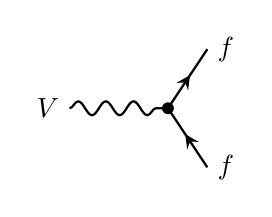
\begin{tikzpicture}[thick]
        \coordinate  (a) at (0,0) ;
        \coordinate  (b) at (1.25,0) ;
        \coordinate  (c) at (1.75,0.75) ;
        \coordinate  (d) at (1.75,-0.75) ;

        \draw[-,boson]  (a) -- (b) node[pos=0.0, left=0pt] {$V$} ;
        \draw[-,fermion]  (b) -- (c) node[pos=1.0, right=0pt] {$f$} ;
        \draw[-,fermion]  (d) -- (b) node[pos=0, right=0pt] {$f$} ;
        \node[circle,fill=black,inner sep=0pt,minimum size=1.5mm] (lala) at (1.25,0) {};
    \end{tikzpicture}        
    \hspace{15pt}
    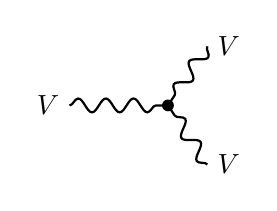
\begin{tikzpicture}[thick]
        \coordinate  (a) at (0,0) ;
        \coordinate  (b) at (1.25,0) ;
        \coordinate  (c) at (1.75,0.75) ;
        \coordinate  (d) at (1.75,-0.75) ;

        \draw[-,boson]  (a) -- (b) node[pos=0.0, left=0pt] {$V$} ;
        \draw[-,boson]  (c) -- (b) node[pos=0.0, right=0pt] {$V$} ;
        \draw[-,boson]  (d) -- (b) node[pos=0, right=0pt] {$V$} ;
        \node[circle,fill=black,inner sep=0pt,minimum size=1.5mm] (lala) at (1.25,0) {};
    \end{tikzpicture}        
    \hspace{15pt}
    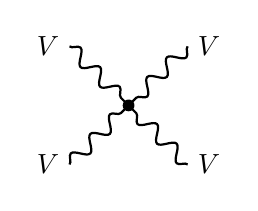
\begin{tikzpicture}[thick]
        \coordinate  (a) at (0,0) ;
        \coordinate  (b) at (-0.75,0.75) ;
        \coordinate  (c) at (-0.75,-0.75) ;
        \coordinate  (d) at (0.75,0.75) ;
        \coordinate  (e) at (0.75,-0.75) ;

        \draw[-,boson]  (b) -- (a) node[pos=0.0, left=0pt] {$V$} ;
        \draw[-,boson]  (c) -- (a) node[pos=0.0, left=0pt] {$V$} ;
        \draw[-,boson]  (d) -- (a) node[pos=0.0, right=0pt] {$V$} ;
        \draw[-,boson]  (e) -- (a) node[pos=0.0, right=0pt] {$V$} ;
        \node[circle,fill=black,inner sep=0pt,minimum size=1.5mm] (lala) at (0,0) {};
    \end{tikzpicture}        
    \caption{The types of possible EW interaction vertices at tree-level (no loops), omitting the diagrams involving a Higgs boson. $V$ represents an EW gauge boson ($\gamma$, $Z$, $W^{\pm}$), $f$ represents a fermion. Care must be taken in the choice of particle, as there are many interactions with the configurations listed here which are not allowed.\label{fig:ewvertices}}
\end{figure} 

\begin{figure}[t]
    \centering
    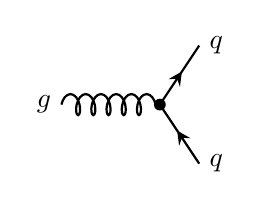
\begin{tikzpicture}[thick]
        \coordinate  (a) at (0,0) ;
        \coordinate  (b) at (1.25,0) ;
        \coordinate  (c) at (1.75,0.75) ;
        \coordinate  (d) at (1.75,-0.75) ;

        \draw[-,gluon]  (a) -- (b) node[pos=0.0, left=0pt] {$g$} ;
        \draw[-,fermion]  (b) -- (c) node[pos=1.0, right=0pt] {$q$} ;
        \draw[-,fermion]  (d) -- (b) node[pos=0, right=0pt] {$q$} ;
        \node[circle,fill=black,inner sep=0pt,minimum size=1.5mm] (lala) at (1.25,0) {};
    \end{tikzpicture}        
    \hspace{15pt}
    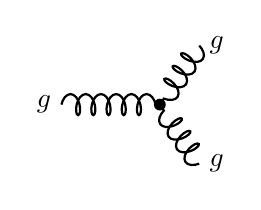
\begin{tikzpicture}[thick]
        \coordinate  (a) at (0,0) ;
        \coordinate  (b) at (1.25,0) ;
        \coordinate  (c) at (1.75,0.75) ;
        \coordinate  (d) at (1.75,-0.75) ;

        \draw[-,gluon]  (a) -- (b) node[pos=0.0, left=0pt] {$g$} ;
        \draw[-,gluon]  (c) -- (b) node[pos=0.0, right=0pt] {$g$} ;
        \draw[-,gluon]  (d) -- (b) node[pos=0, right=0pt] {$g$} ;
        \node[circle,fill=black,inner sep=0pt,minimum size=1.5mm] (lala) at (1.25,0) {};
    \end{tikzpicture}        
    \hspace{15pt}
    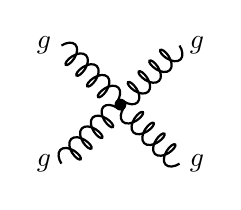
\begin{tikzpicture}[thick]
        \coordinate  (a) at (0,0) ;
        \coordinate  (b) at (-0.75,0.75) ;
        \coordinate  (c) at (-0.75,-0.75) ;
        \coordinate  (d) at (0.75,0.75) ;
        \coordinate  (e) at (0.75,-0.75) ;

        \draw[-,gluon]  (b) -- (a) node[pos=0.0, left=0pt] {$g$} ;
        \draw[-,gluon]  (c) -- (a) node[pos=0.0, left=0pt] {$g$} ;
        \draw[-,gluon]  (d) -- (a) node[pos=0.0, right=0pt] {$g$} ;
        \draw[-,gluon]  (e) -- (a) node[pos=0.0, right=0pt] {$g$} ;
        \node[circle,fill=black,inner sep=0pt,minimum size=1.5mm] (lala) at (0,0) {};
    \end{tikzpicture}        
    \caption{The types of possible QCD (strong) interaction vertices at tree-level, omitting the diagrams involving a Higgs boson. $g$ represents a gluon and $q$ a quark. Since gluons carry colour charge, they can self-interact.\label{fig:qcdvertices}}
\end{figure} 

From Equation \ref{eq:pint}, the probability of an interaction is proportional to the square of the matrix element. Ignoring factors of $2\pi$, this is given by 
\begin{equation}
    |\mathcal{M}|^2=|\mathcal{A}|^2\delta^{(4)}\Bigl(\sum_ip_i-\sum_fq_f\Bigr)\delta^{(4)}(0),
\end{equation}
where $\delta^{(4)}(0)$ comes from the square of the delta function, and results in an infinite interaction probability. This infinity is resolved if a finite space-time volume $VT$ is considered
\begin{equation}
    \delta^{(4)}(0)=\int d^4xe^{-ipx}\Bigr|_{p=0}=\int d^4x=VT.
\end{equation}
%Single-particle states can be normalised according to 
%\begin{equation}
%    \langle p',\lambda'|p,\lambda\rangle=(2\pi)^32E\delta_{\lambda\lambda'}\delta^{(3)}(\mathbf{p}-\mathbf{p}'),\hspace{5pt}E=p^0.
%\end{equation}
After summing over all possible momentum states, the interaction probability per unit time reduces to \cite{Buckley:PCP} 
\begin{equation}\label{eq:almostxs}
    \sum_{\text{momenta}}\frac{P}{T}=\frac{(2\pi)^4}{4E_1E_2V}\Biggl(\prod_{k=3}^{n}\int\frac{\dbar^3\mathbf{p}_k}{2E_k}\Biggr)\delta^{(4)}\Bigl(\sum_ip_i-\sum_fq_f\Bigr)|\mathcal{A}|^2,
\end{equation}
where $E_1$ and $E_2$ are the energies of the initial and final state particles.

$pp$ collision experiments don't directly measure scattering probabilities since the interaction rate depends on factors which are specific to the experiment, such as the focus, shape, and intensity of the particle beams. Instead, a quantity known as the \textit{cross-section} is measured, which is related to scattering amplitudes but is not dependent on the properties of the beam.

%TODO: Something about E1E2, etc.
\subsubsection{Cross-sections}
In a scattering event it is useful to think of one of the particles as being the incident particle, and the other as being the target. Then, there is some region of space around the target particle, such that an interaction occurs if the incident particle is within that region. Therefore the target particle has an effective cross-sectional area for interaction, which is referred to as the scattering \textit{cross-section}, $\sigma$.

The number of scattering events $N$ in a given amount of time is directly related to $\sigma$ and satisfies
\begin{equation}\label{eq:instlumi}
    \frac{dN}{dt}=\mathcal{L}(t)\sigma,
\end{equation}
which defines the quantity known as the \textit{instantaneous luminosity} $\mathcal{L}(t)$ (this is discussed in more detail in Section \ref{sec:lumi}), which carries the dependence on the beam parameters. Linking the interaction cross-section to an event rate requires knowledge of some properties of the incident and target particles, specifically
\begin{equation}\label{eq:xsection}
    \sigma=\frac{1}{N_b\mathcal{F}_a}\frac{\delta N}{\delta t},\hspace{5pt}\text{where}\hspace{5pt}\mathcal{F}_a=n_a(v_a+v_b),
\end{equation}
and $n_a$ is the number of incident particles per unit volume; $N_b$ is the total number of target particles; $v_a,v_b$ correspond to the incident and target particle speeds; and $\mathcal{F}_a$ is the \textit{flux} of the incoming particles.

Scattering processes are described by Poisson statistics since the interaction probability is constant in a given amount of time. For Poisson processes, the total probability per unit time is equal to the event rate. Therefore scattering amplitudes can be linked to cross-sections by taking Equation \ref{eq:almostxs} and dividing by a flux factor. This gives
\begin{equation}
    \sigma=\frac{1}{F}\int d\Phi|\mathcal{A}|^2,\hspace{5pt}\text{where}\hspace{5pt}F=4(E_1|\mathbf{p}_2|+E_2|\mathbf{p}_1|),
\end{equation}
and 
\begin{equation}
    \int d\Phi=(2\pi)^4\Bigl(\prod_k\int\frac{\dbar^3\mathbf{p}_k}{2E_k}\Bigr)\delta^{(4)}\Bigl(\sum_ip_i-\sum_fq_f\Bigr),
\end{equation}
where $F$ is referred to as the Lorentz invariant flux, the product is over final state particles, and $\int d\Phi$ is the phase-space integral.
The calculation of a scattering cross-section is therefore performed by (i) calculating the square modulus of the scattering amplitude $\mathcal{A}$, (ii) performing the phase-space integral, and (iii) dividing by a flux factor. 
% Maybe worth mentioning needing to average over colours and spins?????

Chapter \ref{sec:vbswy} outlines the measurement of a \textit{differential} cross-section. This describes the dependence of $\sigma$ with a some observable $\mathcal{O}$, and is denoted $\frac{d\sigma}{d\mathcal{O}}$. Experimentally, this is determined through measuring the number of scattering events in a given bin of the observable, and normalising by the integrated luminosity (Section \ref{sec:lumi}).

\subsection{Calculations of Cross-sections in $pp$ Collisions}

The methods described above allows for the calculation of cross-sections for the scattering of two fundamental particles. However, it is not immediately obvious how to extend this prescription to $pp$ collisions. A proton is a bound state of three quarks, $uud$, where the binding force is the strong interaction, or QCD. One of the properties of QCD is that the interactions become asymptotically weaker at higher energies (equivalently, smaller times or distances), this is called \textit{asymptotic freedom}. Hence, for the high-energy collisions at the LHC, protons interact as if their constituents are not in a bound state at all. 

Due to the Heisenberg uncertainty principle, the constituent valence quarks\footnote{The valence quarks are the real $uud$ quarks that make up the proton. However, the proton mass is much larger than the sum of the valence quark masses. Therefore it is useful to think of a proton as consisting of \textit{partons}, which describes a valence quark, gluon, or a virtual quark (known as a \textit{sea quark}).} of the proton have non-zero momenta, even in the rest frame of the proton. In the proton rest frame, the extreme case can be considered where the energy of one of the valence quarks is equal to half of the proton mass. A Lorentz boost to the lab frame then reveals that the quark momentum can take any value between zero and the total proton momentum. Therefore it is useful to think of colliding partons as having a momentum collinear with the proton $p_i$ which is some fraction $x_i$ of the total proton momentum $P_i$
\begin{equation}
    p_i=x_iP_i,\hspace{5pt}0\leq x_i\leq1.
\end{equation}
Individual cross-sections for quarks and gluons can then be combined in the following way to give the total cross-section $\sigma$ corresponding to a $pp$ collision
\begin{equation}
    \sigma=\sum_{i,j\in\{q,\bar{q},g\}}\int_{0}^{1}dx_1\int_{0}^{1}dx_2f_i(x_1)f_j(x_2)\hat{\sigma}{}_{ij},
\end{equation}
where the sum is over all combinations of partons, and $\hat{\sigma}{}_{ij}$ is the cross-section for a given parton scattering process, referred to as the \textit{partonic cross-section}. The functions $f_i(x_k)$ are called parton distribution functions (PDFs) which are probability distributions that give the probability of there being a parton $i$ with momentum fraction $x_k$ in proton $k$. The total cross-section $\sigma$ is therefore split up into a part which can be calculated using perturbation theory -- the partonic cross-sections -- and a part which cannot be calculated using perturbation theory, and must be determined from the particle collision data -- the PDFs. It is worth pointing out that this treatment of PDFs is a simplification, and in particular, PDFs can be negative at next-to-leading and higher orders. The true form of the hadronic cross-section is written as
\begin{equation}\label{eq:fullfact}
    \sigma=\sum_{i,j\in\{q,\bar{q},g\}}\int_{0}^{1}dx_1\int_{0}^{1}dx_2f_i(x_1,\mu_{\mathrm{F}}^2)f_j(x_2,\mu_{\text{F}}^2)\hat{\sigma}{}_{ij}(x_i,\mu_{\mathrm{F}}^2,\{p_i\cdot p_j\})+\mathcal{O}\left(\frac{\Lambda^2_{\text{QCD}}}{Q^2}\right),
\end{equation}
which includes a momentum transfer scale describing the partition between the perturbative and non-perturbative physics, the factorisation scale $\mu_{\mathrm{F}}$ (more detail in Section \ref{sec:formhad}). Equation \ref {eq:fullfact} also contains a dependence on the energy scale of the hard scattering process, $Q^2$, and the scale at which the strong coupling becomes large, $\Lambda_{\text{QCD}}$. 
Variations in the PDFs and factorisation and renormalisation\footnote{The renormalisation scale is a factor which enters into the running of the masses and the coupling constant in QCD. For more detail refer to \cite{Buckley:PCP} and Section \ref{sec:vbswy:theoryunc}.} scales are used to estimate uncertainties in theory predictions, for more details refer to Section \ref{sec:vbswy:theoryunc}.
% Now PDFs.
% 2. Bring in PDFs. These allow us to calculate cross-sections for processes in pp collisions. Then talk about how partons in final state will form hadronic systems -- The parton shower is/are an approximation to this. Perturbation theory is used, typically at NLO accuracy, sometimes only leading order. 
% 3. Hadronisation part (call this ``formation of hadronic final states'') -- ``catch-22 situation'' Andy suggested looking at how others resolve this...  Concept of PS is more a MC method. Parton shower -- [describes the?] dominant physics process. The ME diverges at small angles, this is the origin of parton shower. Not too many details on how hadronisation works. Should describe how to get from collisions to a stream of partons to hadrons. Should describe the divergence in the matrix element -- high virtuality -- [makes the final states?] likely to split into multiple partons.
% 4. Subsection on MC. (around 2 pages?) Partonic cross-section calculation at NLO using: [multiplicity??] merging, parton shower and hadronisation algorithms, underlying event and MPI. Then discuss what the state of the art in simulation is. Should discuss PS and hadronisation as a concept [I guess in the previous subsection] and then here go into the algorithms for the PS and hadronisation models e.g. PT ordering/angular ordering in pythia/herwig etc. 
%subsubsection on jets -- see ste
% Small angle/collinear divergences: consider soft radiation of a gluon off an external quark line, QCD feynman rules give the propagator as 1/p^2 (given xyz assumptions). Then can choose a frame such that .... Soft and collinear result in IR divergences. 

\subsection{Formation of Hadronic Final States}\label{sec:formhad}

Even if it is possible to calculate the partonic cross-section for a given scattering process at a fixed order in perturbation theory and combine these with PDFs to get a hadronic cross-section, there are still a substantial number of complexities to consider before arriving at a result which can be compared with experimental data. It turns out it is not possible to describe the hadronic final state solely using perturbation theory. In practise then, the hadronic final states are simulated using \textit{Monte Carlo} (MC) event generators, where MC refers to a class of statistical techniques used in the simulations.

In any given $pp$ collision at the LHC, the incoming partons can radiate gluons and since those gluons are colour charged, they can go to radiate even further. There is therefore a huge amount of QCD radiation from the incoming partons prior the hard interaction (i.e. the process where a large momentum transfer occurs or where heavy objects are created) in addition to radiation from the outgoing partons. Calculating the Feynman diagrams corresponding to each emission is clearly not practical. In practise, MC event generators employ \textit{parton shower} algorithms to model this QCD radiation. At a certain point, the partons cease to radiate. Since free partons cannot exist due to a property of QCD known as \textit{confinement}, they go on to form colour neutral (singlet) bound states, hadrons, before they can be observed. The formation of hadrons from partons is called \textit{hadronisation}, and occurs when the momentum transfer scale is small. This in turn means that the value of strong coupling $\alpha_s$ is large. In this regime, perturbation theory breaks down as it relies on $\alpha_s$ being small. Hadronisation, therefore, is intrinsically non-perturbative. In describing the hadronic final state, MC generators employ hadronisation models to describe this non-perturbative physics.

\subsubsection{Parton Showers and Hadronisation}

The description of parton showers begins with the observation that partonic cross-sections tend to diverge when we consider soft or collinear (small-angle) radiation. Consider a $q\bar{q}$ scattering process where there is additional gluon radiation off of an incoming external quark leg. If the quark has momentum $p_1$ and the radiated gluon has momentum $k$, there is an additional internal quark leg whose propagator\footnote{In the QCD Feynman rules an internal leg corresponds to a factor of $\frac{i(\slashed{p}+m)}{p^2-m^2+i\epsilon}$, where $\epsilon\ll1$ insures the correct causal properties. This factor is called the propagator. For the calculation in this section, the quark is assumed to be massless.} contains the factor 
\begin{equation}\label{eq:medivergence}
    \frac{1}{(p_1-k)^2}=\frac{1}{-2|\mathbf{p_1}||\mathbf{k}|(1-\cos{\theta})},
\end{equation}
where the last equality holds when we consider the lab frame at a $pp$ collider, and the gluon momentum is parametrised in terms of a $qg$ scattering angle $\theta$, i.e.
\begin{equation}
    p_1^{\mu}=(|\mathbf{p_1}|,0,0,|\mathbf{p_1}|),\hspace{5pt}k^\mu=(|\mathbf{k}|,0,|\mathbf{k}|\sin{\theta},|\mathbf{k}|\cos{\theta}).
\end{equation}
The scattering amplitude diverges in the soft and collinear limit. The problem here lies in that this calculation pertains to a scattering amplitude for a process where the final state has a fixed number of partons. This amplitude is not \textit{infrared safe} (IR safe) as it does not include a sum over all physically indistinguishable states. For the case of $pp$ collisions, all partonic cross-sections are not IR safe by themselves. This is because there are divergences associated with not summing over all possible initial states. The total hadronic cross-section is IR safe however, as the IR divergences are absorbed by the PDFs by defining a momentum transfer scale $\mu_F$, called the factorisation scale which effectively divides the perturbative from the non-perturbative physics. In simulating scattering events $\mu_F$ must be set at some fixed choice. %Probably something about muR would be good as well... 

Let's consider the case where a final state parton $i$ radiates and therefore splits into other partons, $j$ and $k$. In turns out that in the collinear limit, the partonic differential cross-section for the $n+1$ parton production factorises into the differential cross-section for $n$ parton production multiplied by a factor that includes a sum over all partons that give final state parton $j$. 
\begin{equation}\label{eq:factorisation}
    d\hat{\sigma}{}_{n+1}=d\hat{\sigma}_n\sum_i\int_{k_{\text{min}}}^{k_{\text{max}}}\frac{d|\mathbf{k}_{T}|^2}{|\mathbf{k}_{T}|^2}\int_{z_{\text{min}}}^{z_{\text{max}}}\frac{dz}{z}P_{ji}(z),
\end{equation}
where $\mathbf{k}_T$ is the transverse momentum of the parton $k$ relative to $j$, $P_{ji}$ are \textit{splitting functions} which are different depending on the specific parton splitting vertex and depends on $\alpha_s$ and $z$, which is the fraction of the momentum of parton $i$ carried by parton $j$. Equation \ref{eq:factorisation} makes it possible to calculate the differential partonic cross-section for any number of collinear splittings. Even if the splittings are not exactly collinear, this will give a reasonable approximation since radiation is enhanced in the collinear limit. 

With each emission, the emitting parton gets progressively closer to satisfying 
\begin{equation}
    t\equiv p_i^2=0,
\end{equation}
where the \textit{virtuality} $t$ is defined as the square of the momentum of parton $i$, and the parton is assumed to be massless. This means that the parton gets progressively closer to being on-shell. However, because of colour confinement, the parton will never be precisely on-shell, therefore the parton ceases to emit at a certain virtuality, $t_0$. The probability of an emission between virtualities $t_n$ to $t_{n+1}$ for momentum fractions $z_n$ and $z_{n+1}$ is given by the probability of no (resolvable) emissions in the virtuality range multiplied by the probability of a (resolvable) emission which is related to the splitting function for the pair $(z_n, z_{n+1})$. The probability for a whole cascade of partons is just given by repeated products of these terms. Therefore a parton shower algorithm can simulate QCD radiation through randomly generating a set of virtualities and momentum fractions.

Thus far we have only considered radiation in the small angle limit, but Equation \ref{eq:medivergence} shows that soft radiation is also enhanced. For wide-angle soft radiation, the differential cross-section does not factorise like in Equation \ref{eq:factorisation}. However, the resolution to this is relatively straightforward. By ordering the parton shower in emission angle $\theta$ rather than virtuality, the effects of soft emissions are correctly accounted for -- this is called \textit{angular ordering}. Another resolution is to replace the notion of radiation recoiling off a single parton with recoil against a pair of partons. This is called a \textit{dipole shower}. Depending on the MC generator, either transverse-momentum ordered dipole showers or angular ordering are used in parton shower algorithms.

In the current description of the formation of the partonic final state is an unaddressed ambiguity relating to whether the additional partonic radiation should be generated from the matrix element or from the parton shower. Since the parton shower is only exact for collinear radiation, it does not provide a good description of wide-angle radiation. Therefore it is preferable not to leave the generation of additional partons entirely up to the parton shower. On the other hand, the matrix element calculations contain collinear singularities, meaning that additional small-angle radiation is not well described by higher order calculations in the matrix element. The \PYTHIA user manual \cite{Theory:Pythiamanual} defines the procedure of combining one matrix element calculation with the parton shower as \textit{matching}, and combining several matrix element calculations with each other and the parton shower as \textit{merging}.

The formation of final state hadrons from a collections of partons is modelled through hadronisation algorithms. The two primary models are called the \textit{Lund string model} and the \textit{cluster} hadronisation model. The Lund string model is predicated on the fact that the strong force between a quark-antiquark pair is constant with the distance between them if they are sufficiently far apart. The gluon field lines between the quarks are called \textit{flux tubes} (or \textit{strings}) with uniform energy per unit length. At a large enough separation, the flux tube breaks resulting in the formation of another quark-antiquark pair. Hadrons are formed by the grouping of quarks when a string splitting is no longer kinematically possible. The model depends on a number of parameters which affect the functions describing the momenta of the quarks after a string break and the probability distributions governing a string break. In the cluster model, the gluons at the end of the parton shower split up into quark-antiquark pairs. Subsequently, colour neutral clusters are formed from neighbouring quark-antiquark pairs, which then go on to decay into hadrons. 
%Tomorrow matching/merging MPI UE and jets. 

The description of a hadronic scattering process given here still does not include a number of complexities such as the interactions between multiple incoming partons -- called multi-parton interactions (MPI) -- and effects of the proton remnants. Such additional complexities which are not considered in the hard scatter, parton shower, or hadronisation are collectively referred to as the \textit{underlying event} (UE). Accurate modelling of the UE is often very important in comparing predictions with experimental data \cite{Buckley:evgens}. % A little bit a bout matching and merging? 

\subsubsection{Jet Formation}\label{sec:theory:jet}

The hadrons produced as a result of the $pp$ collisions at the LHC are grouped into collimated streams of hadrons called jets. The reason for this is that the hard interaction gives rise to high transverse momentum partons which then go on to emit approximately collinear radiation. The kinematics of the resulting jet is then closely related to that of the original hard parton \cite{Atlas:Salam2009}. Jets are defined using by a specific \textit{jet algorithm}, which is a set of rules that govern the grouping of partons. Simulated and measured collision events can then be readily compared if the same algorithm is used for both. The primary requirement of a jet algorithm is that it should be IR safe, meaning that the addition of soft and/or collinear emissions should not change the results. 

The jet algorithm that is primarily used at the LHC is the anti-$\kt$ algorithm \cite{Insitu:antikt}. This algorithm falls under a class of IR safe algorithms known as \textit{sequential recombination} algorithms which both find jets and assign a clustering sequence to an event. In these algorithms, pairs of particles are grouped together according to the value of a distance parameter. In the anti-\kt algorithm, the distance parameter is based on the transverse momenta of the particles. This choice is motivated by the observation that the parton multiplicity of a jet depends on its transverse momentum \cite{Atlas:Lee,Atlas:Dokshitzer,Atlas:Catani}.

The anti-\kt algorithm uses a particle distance parameter $d_{ij}$ and an additional beam distance parameter $d_{iB}$. 
\begin{subequations}\label{eq:dijdib}
\begin{equation}\label{eq:dij}
    d_{ij}=\min(p^{2p}_{t,i},p^{-2}_{t,j})\frac{\Delta R^2_{ij}}{R^2},\hspace{15pt}\Delta R^2_{ij}=(y_i-y_j)^2+(\phi_i-\phi_j)^2,
\end{equation}
\begin{equation}\label{eq:dib}
    d_{iB}=p^{-2}_{t,i},
\end{equation}
\end{subequations}
where the $R$ parameter is related to the radius of the jet and is usually set at $R=0.4$ at ATLAS. $\phi_i$ and $y_i$ denote the azimuthal angle and rapidity (defined in Chapter \ref{sec:atlasdetector}) of the particle.
%If a hard parton has no hard neighbors within a distance $2R$, then all soft particles will be accumulated around it within a circle of radius $R$ resulting in a perfectly conical jet \cite{Cacciari:2008gp}

The anti-$k_t$ algorithm favours clustering around hard seeds and produces circular jets \cite{Cacciari:2008gp}. This is attractive because soft hadrons which are produced from the emissions of a hard parton ought to be assigned to the jet of the nearest hard parton \cite{Atlas:Catani}. Circular jets are desired since any jet that points at least a distance $R$ from the edge of the center of the detector will then be fully contained within it \cite{Atlas:Salam2009}.

\subsubsection{Monte-Carlo Event Generators}
% Powheg, Pythia, Madgraph, Sherpa
%Monte-Carlo event generators are responsible for simulating the $pp$ collisions. 
The generation of simulated events in Monte-Carlo (MC) event generators begins with the matrix element calculation of a user-selected hard process at a given order in perturbation theory which is typically at NLO. In order to calculate a cross-section, the square of the matrix element needs to be derived for every phase-space point (the set of incoming and outgoing momenta). There is the possibility of relying on analytical results for LO matrix elements for low multiplicity final states (usually 1-3 particles), and all multi-purpose MC event generators rely on such a list of LO matrix elements. Alternatively, dedicated matrix-element and phase-space generators exist for the calculations involving more complex final states. Some examples are the \ALPGEN \cite{Theory:alpgen}, \AMEGIC \cite{VBSWy:amegic}, or \COMIX \cite{Insitu:comix} programs.% Performing the matrix element calculation requires a sum over quantum numbers such as helicity and colour of the incoming and outgoing particles. Where there is choice to either sum over all quantum numbers or to randomly sample them \cite{Buckley:evgens}. 

After the construction of the matrix element, the phase-space integrals are usually computed using algorithms which rely on phase-space sampling. Examples of such algorithms are \textit{sequential} algorithms which rely on the pole structure of one of the Feynman diagrams contributing to the matrix element \cite{Theory:sequential} and \textit{multi-channel} integrators which utilise combinations of several sampling algorithms \cite{Theory:multichannel}. Because of the large dimensionality of the phase-space, numerical techniques such as quadrature integration are not typically not practical for the computation of phase-space integrals \cite{Buckley:evgens}.

Subsequent to the simulation of the hard interaction, MC event generators are also responsible for simulating the parton showers associated with incoming and outgoing partons, performing hadronisation algorithms, simulating underlying-event activity, and modelling the decays of unstable particles. 

The primary event generators used for event simulation in the analyses described in Chapters \ref{sec:insitu} and \ref{sec:vbswy} are \POWHEG \cite{Insitu:powheg1,Insitu:powheg2,Insitu:powheg3}, \PYTHIA \cite{Theory:Pythiamanual,Insitu:pythia}, \SHERPA \cite{Insitu:sherpa,Insitu:sherpa22}, and \MADGRAPH \cite{VBSWy:madgraph}. For the MC samples used in this thesis, when matrix elements are calculated using \POWHEG and \MADGRAPH, they are interfaced with \PYTHIA for parton showering and hadronisation, whereas samples generated using \SHERPA use the same program for parton showering and hadronisation. \PYTHIA and \SHERPA both have \pt-ordered dipole showers, but \PYTHIA uses the lund string model for hadronisation, whereas \SHERPA uses the cluster model. \MADGRAPH, \SHERPA, and \POWHEG all use different schemes for the matching and merging of matrix elements with parton showers \cite{Insitu:ckkw1,Insitu:ckkw2,Theory:MLM}, where for NLO matching and merging, \MADGRAPH uses the MC@NLO implementation \cite{Theory:MCnlo}, \SHERPA uses a variant of this \cite{Theory:sherpamatching}, and \POWHEG has its own dedicated approach \cite{Insitu:powheg3}.
%Pythia: often interfacted for ps/had - CHECKED.
% Pythia and sherpa have pt-ordered dipole showers
% Pythia uses lund string model, Sherpa uses cluster model
% Madgraph MLM matching scheme, Sherpa CKKW matching scheme
% NLO matching schemes: MC@NLO madgraph, sherpa uses variant of MC@NLO. POWHEG has its own approach. Difference 
%Still want to discuss: MC truth, matching and marging, (maybe particle level), different generators, NLO calculations
%
% It turns out that the probability of a sequence of emissions is parametrised by a set of momentum fractions $z_i$ and virtualities $t_i$ through probability functions known as \textit{Sudakov form factors}. A parton shower can then be simulated by generating a set of $(t_0,t_i,z_i)$
%Parton shower:
%Radiation is enhanced if it is soft and/or collinear. Partonic differential cross-section for parton i->jk splitting factorises in the limit of j and k being collinear. This means dsigma_n+1 ~ dsigma_n * (something). Something is related to deglap functions for i->jk splitting. Suggests extra parton ``k'' is independent of the rest of the process. This argument can be repeated for a whole load of collinear emmissions. All of these arguments rely on the assumption that the radiation is collinear with one of the original hard partons (the well seperated partons in the final state), in this situation can describe the radiation EXACTLY. In reality, partons have non-zero angle, but we known radiation is ENHANCED in the collinear limit. Therefore collinear limit rives reasonable approximation for extra radiation.
%The parton shower represents an approximate perturbative treatment of QCD dynamics at scales of mo- mentum transfer-squared t greater than some infra-red cut-off value t0, typically taken to be of the order of 1 GeV 2 . The Monte Carlo method is particularly convenient because the perturbative treatment at t > t0 can be combined with a non-perturbative model of the hadronization process, assumed to take place at scales t < t0. In this way one obtains a QCD event generator, -- "qcdandcolliderphysics.pdf page 157"
%U hadronic final states in high energy colliders such as the LHC 
%Calculating the scattering amplitudes for all of these possible interactions using the Feynman rules is clearly not feasible. Additionally,  Confinement cannot be  is intrinsically non-perturbative 
%which acts as a cutoff on the transverse momentum integral ... We can then think of µF as some “dividing scale”, that separates perturbative from non-perturbative physics i.e. if |kT | > µF , then a radiated parton is perturbative, but if |kT | < µF it is non-perturbative, and thus sensitive to the strongly coupled dynamics that holds the proton together. Such emissions should then be part of the PDF rather than the partonic cross-section. ... The factorisation scale µF is arbitrary. However, once we have fixed a choice, we can measure the PDFs from data.
%Not clear from above how to deal with incoming protons. Asymptotic freedom suggests (for fast moving protons) q/g can leave proton and collide. Refer to p29 of PoTU notes about asymptotic freedom. A little bit about partons in general, talk about valence and sea quarks -- can maybe refer to PoTU notes. Maybe also a little intro about why we care i.e. MC generators. In partonic cross-section model the partonic cross-section describes the thing that can be calculated in perturbation theory, and the non-perturbative physics is described by the PDFs. PDFs are probability distributions because a-priori cannot determine energy fraction of a given parton because of uncertaintiy principle. PDFs "absorbs the non-perturbative diver-gences by using the factorisation scale". Factorisation scale P94 PCP. When mentioning IR divergences, worth mentioning UV divergences in passing (refer to page 77 PCP). Need to mention somewhere what "fixed-order perturbation theory" means exactly.
% Small angle/collinear divergences: consider soft radiation of a gluon off an external quark line, QCD feynman rules give the propagator as 1/p^2 (given xyz assumptions). Then can choose a frame such that .... Soft and collinear result in IR divergences. 
%The resolution to this is that QUOTE "not all theoretical observables are physically meaningful: only those that are infrared safe. Such observables include a sum over all physically indistinguishable states" ENDQUOTE Another good quote: QUOTE "Another way of defining an infrared safe observable is that it should be well-behaved upon adding an additional soft particle, or splitting a partoninto two collinear ones. Fixing the number of partons in the final state, as we did above in equation (2.200) fails this definition, and thus σqq̄g is not IR safe by itself. This is why equation (2.201) contained infrared divergences." ENDQUOTE-- page 92 PCP.
% For non-Abelian theories IR singularities do cancel, but only if we include initial states with ANY number of particles. But in pp collisions only ever have two initial states, therefore uncancelled IR singularities from ISR. Partonic cross-sections become unphysical. This is resolved when combining partonic cross-sections with PDFs. 
%Need to mention UV divergences and renormalisation scale somewhere
%PCP 94: PDFs are not physical by themselves: the only directly measurablequantity is the hadronic cross-section σ, which combines the PDFs with the partonic cross-section. Thus, we are free to move contributions from the partonic cross-section into the PDFs if we want to. By doing so, we can remove the collinear singularity! ... We see that equation (2.217) no longer has a collinear singularity as k k p1 . It has been removed by the factorisation scale µF , which acts as a cutoff on the transverse momentum integral ... We can then think of µF as some “dividing scale”, that separates perturbative from non-perturbative physics i.e. if |kT | > µF , then a radiated parton is perturbative, but if |kT | < µF it is non-perturbative, and thus sensitive to the strongly coupled dynamics that holds the proton together. Such emissions should then be part of the PDF rather than the partonic cross-section. ... The factorisation scale µF is arbitrary. However, once we have fixed a choice, we can measure the PDFs from data.
%Buckleys pdf: DIRECTQUOTE!! "The cross section defined by Eq. (1) is fully specified only for a given PDFset and a certain choice for the unphysical factorization and renormalization scales. There exists no first principle defining what are the correct μF and μR. However, our knowledge of the logarithmic structure of QCD for different classes of hard scattering processes limits the range of reasonable values. This knowledge is used as a guide when setting the default choices in the various generators" DIRECTQUOTE
% Particlephyiscs p95: ...which absorbs the non-perturbative diver-gences by using the factorisation scale.
%TODO: Would like to have a little paragraph explaining what "truth-level" "particle-level" "reco-level" etc is. Probably in the MC part

\section{Vector Boson Scattering}\label{sec:vbs}

Precision measurements of processes involving Vector Boson Scattering (VBS) and Vector Boson Fusion (VBF) have become experimentally measurable only very recently, with the first measurements by ATLAS and CMS in LHC Run-1 \cite{VBSWy:VBS1,VBSWy:VBS2,VBSWy:VBS3,VBSWy:CMSVBSWy,VBSWy:VBS5,VBSWy:VBS6,VBSWy:VBS7}. The defining feature of VBS and VBF processes is the t-channel exchange of an EW gauge boson in a quark/anti-quark scattering processes. The presence of one (two) EW boson(s) in the final state is referred to as VBF (VBS). The two final-state quarks are manifested as hard \textit{tagging} jets in the forward and backward regions of the detector. Moreover, these events are characterised by the lack of hadronic activity in the rapidity interval of the tagging jets, centrally produced EW bosons, and a large dijet mass \mjj of the tagging jets. 

Measurements of VBS processes are of particular interest because the production cross-section is sensitive to Feynman diagrams which include quartic EW boson (Z,W,$\gamma$) self-interactions.\footnote{It is important to note that the full gauge invariant set of Feynman diagrams contributing to the scattering cross-section includes those contributions from non-VBS interactions. Therefore, it is not possible to solely measure the VBS interactions.} The scattering cross-section in VBS processes also include contributions from trilinear interactions, but since these can be probed through more common diboson processes, the primary goal in measuring VBS is to study the quartic vertices. These cross-sections are usually of the order of fb, and therefore represent some of the rarest processes which are still measurable at the LHC. 

Chapter \ref{sec:vbswy} outlines the differential cross-section measurement of $W\gamma$ production in association with two jets. This process is sensitive to VBS interactions, and occurs with electroweak (EW) and strong production modes. The EW production mode is defined by tree-level diagrams calculated at $\mathcal{O}(\alpha_{\text{EW}}^4)$, and include diagrams with the t-channel exchange of an EW boson and (s-channel) triboson production. The strong production mode has tree-level diagrams at $\mathcal{O}(\alpha_{\text{s}}^2\alpha_{\text{EW}}^2)$ and includes diagrams where quarks and gluons are exchanged in the t-channel. Some examples of tree-level diagrams for the EW and strong production modes are shown in Figure \ref{fig:vbswy:diagrams}. The rate of the strong production mode is significantly higher than the EW production mode because of the appearance of two powers of the strong coupling constant and the larger number of subprocesses that contribute to the total cross-section. It is for this reason that the dominant systematic uncertainties associated with VBS measurements usually pertain to the modelling of the strong background. A precise measurement of the EW production mode therefore requires this background to be carefully constrained.

The lack of central hadronic activity for VBS processes is a feature of perturbative QCD, and is a  consequence of the colour structure \cite{Plehn:2009nd}. In the tree-level VBS diagrams in Figure \ref{fig:vbswy:diagrams}, it is only colour singlet states that are exchanged through the rapidity difference of the two partons. Therefore the dominant contributions to the EW process are the t-channel diagrams which do not have any colour exchange between the partons. This results in the outgoing quarks being only slightly deflected, and the emission of any partons will be therefore be along the beamline. For the strong diagrams (for example diagram (f) in Figure \ref{fig:vbswy:diagrams}), a colour charge is accelerated through the rapidity difference of the incoming partons, which will generate parton radiation away from the beamline. A central jet veto is therefore paramount in separating the VBS signal from large strong backgrounds. Because of the lack of central hadronic activity, the outgoing quarks in a VBS interaction will have a back-to-back geometry with large longitudinal momenta. This motivates the requirements of a large dijet mass and rapidity separation. 

%Higher order diagrams that involve the exchange of a virtual gluon are almost entirely absent from phase-space arguments since this would require one of the forward jets to ``go backwards''. Additionally, diagrams with such a gluon exchange only contribute with a non-zero colour factor if the final state quarks are identical \cite{Plehn:2009nd}. Therefore, these diagams are not likely to correspond to the hard interaction since they must involve a sea quark.

%
%
%\begin{figure}[t]
%    \centering
%    \begin{tikzpicture}[thick]
%        \coordinate  (a) at (0,0) ;
%        \coordinate  (b) at (1.25,0) ;
%        \coordinate  (c) at (1.75,0.75) ;
%        \coordinate  (d) at (1.75,-0.75) ;
%        \coordinate  (e) at (2.5,-0.75) ;
%        \coordinate  (f) at (1.25,-1.50) ;
%        \coordinate  (g) at (0,-1.50) ;
%        \coordinate  (h) at (1.75,-2.20) ;
%
%        \draw[-,fermion]  (a) -- (b) node[pos=0.0, left=0pt] {$q_1$} ;
%        \draw[-,fermion]  (b) -- (c) node[pos=1.0, right=0pt] {$q_1'$} ;
%        \draw[-,boson]  (b) -- (d) node[pos=0.3, right=2.0pt] {$W^+$} ;
%        \draw[-,higgs]  (e) -- (d) node[pos=0, right=0pt] {$h$} ;
%        \draw[-,boson]  (f) -- (d) node[pos=0.3, right=2.0pt] {$W^-$} ;
%        \draw[-,fermion]  (g) -- (f) node[pos=0.0, left=0.0pt] {$q_2$} ;
%        \draw[-,fermion]  (f) -- (h) node[pos=1.0, right=0pt] {$q_2'$} ;
%        \node[circle,fill=black,inner sep=0pt,minimum size=1.5mm] (lala) at (1.25,0) {};
%        \node[circle,fill=black,inner sep=0pt,minimum size=1.5mm] (lala) at (1.75,-0.75) {};
%        \node[circle,fill=black,inner sep=0pt,minimum size=1.5mm] (lala) at (1.25,-1.50) {};
%    \end{tikzpicture}        
%    \caption{Higgs production via vector boson fusion of $W^+W^-$. \label{fig:vbfh}}
%\end{figure}

\begin{figure}[t]
\centering
\begin{subfigure}[b]{0.32\textwidth}
    \centering
    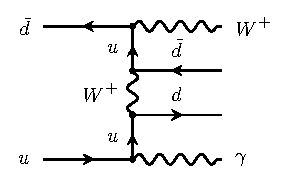
\includegraphics[width=\textwidth]{plots/diffx/vbswgEW1.pdf}
    \caption{}
\end{subfigure}
\hfill
\begin{subfigure}[b]{0.32\textwidth}
    \centering
    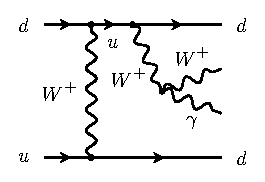
\includegraphics[width=\textwidth]{plots/diffx/vbswgEW2.pdf}
    \caption{}
\end{subfigure}
\hfill
\begin{subfigure}[b]{0.32\textwidth}
    \centering
    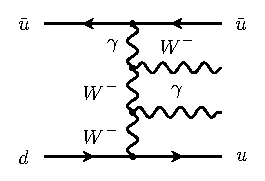
\includegraphics[width=\textwidth]{plots/diffx/vbswgEW4-1.pdf}
    \caption{}
\end{subfigure}
\hfill
\begin{subfigure}[b]{0.32\textwidth}
    \centering
    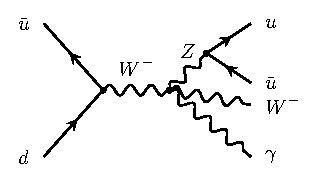
\includegraphics[width=\textwidth]{plots/diffx/vbswgEW5-1.pdf}
    \caption{}
\end{subfigure}
\hfill
\begin{subfigure}[b]{0.32\textwidth}
    \centering
    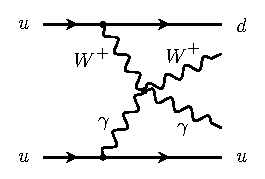
\includegraphics[width=\textwidth]{plots/diffx/vbswgEW3.pdf}
    \caption{}
\end{subfigure}
\hfill
\begin{subfigure}[b]{0.32\textwidth}
    \centering
    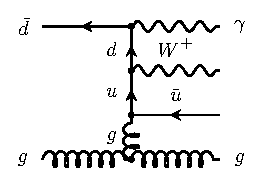
\includegraphics[width=\textwidth]{plots/diffx/vbswgQcd.pdf}
    \caption{}
\end{subfigure}
\caption{(a) \ewwy production involving no gauge boson self-interactions; (b) bremsstrahlung \ewwy non-VBS production involving trilinear gauge boson interactions; (c) \ewwy VBS involving trilinear gauge boson interactions; (d) \ewwy non-VBS production through s-channel triboson interaction involving EW quartic gauge boson interactions; (e) \ewwy VBS involving quartic gauge boson interactions; (f) \qcdwy production. Diagrams produced by author apart from (b) and (e), which are from \cite{VBSWy:VBSWy}.\label{fig:vbswy:diagrams}}
\end{figure}

\subsubsection{Status of VBS Measurements at ATLAS}

A summary of the standard model fiducial and total cross-section measurements derived at ATLAS are shown in Figure \ref{fig:smxsections}. From this figure it is clear that the VBS and VBF measurements correspond to some of the rarest standard model processes measured at ATLAS. In addition to electroweak $W\gamma jj$, some of the most recent VBS-sensitive measurements include 
\begin{itemize}
    \item The fidual cross-section measurement and observation of electroweak $W^{\pm}W^{\mp}jj$ production \cite{Theory:opsignww};
    \item The electroweak and inclusive differential cross-section measurements of $W^{\pm}W{\pm}jj$ production \cite{Theory:samesignww};
    \item Electroweak and inclusive differential cross-section measurements of $ZZ(\rightarrow4\ell)jj$ \cite{Theory:zzfourl}.
\end{itemize}
A summary of all public VBF, VBS, and triboson cross-section measurements, and their agreement with theory are shown in Figure \ref{fig:smvbsmeasurements}.

\begin{figure}
    \centering
    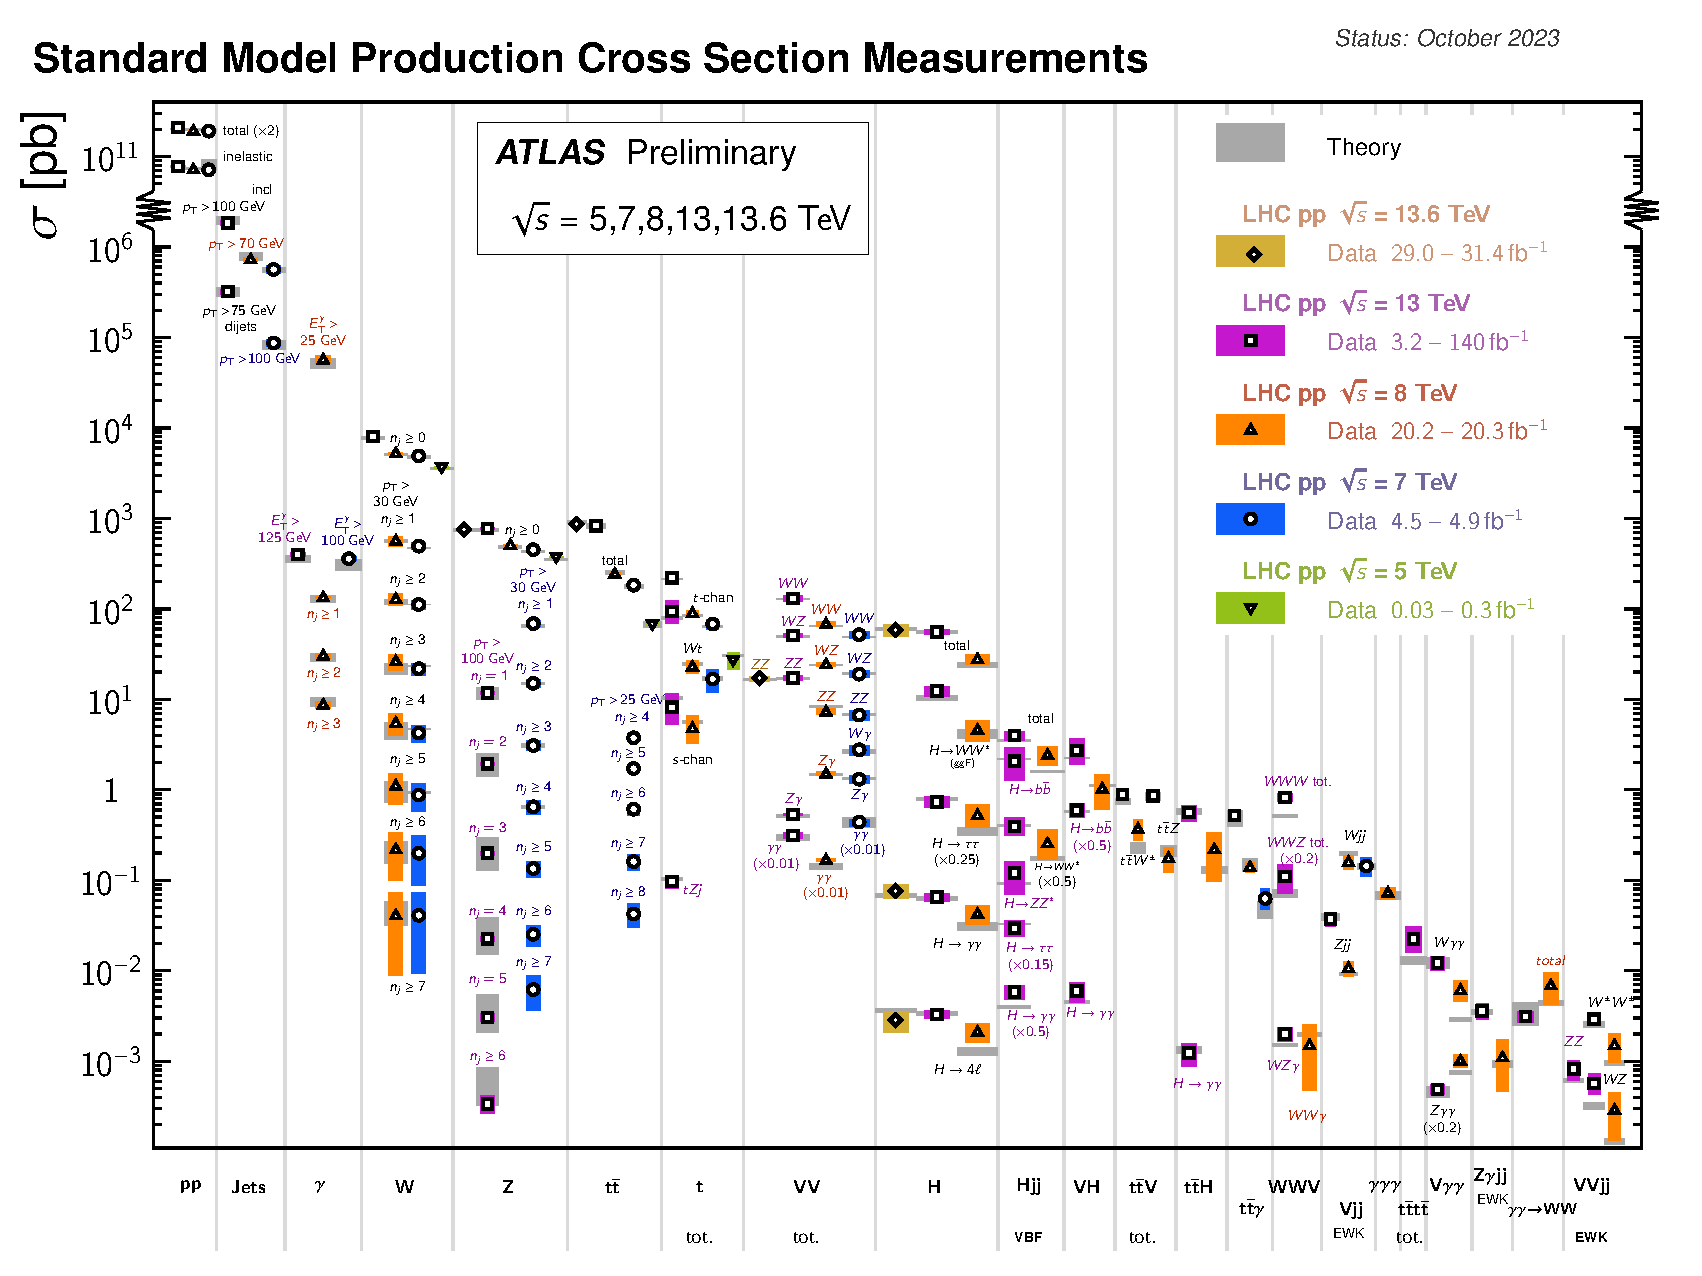
\includegraphics[width=\textwidth]{plots/theory/SM_summary_xsections.pdf}
    \caption{Overview of standard model total and fiducial cross-section measurements made at ATLAS. Total cross-sections are corrected for branching fractions. Figure from \cite{Theory:AtlasSummary}.\label{fig:smxsections}}
\end{figure}

\begin{figure}
    \centering
    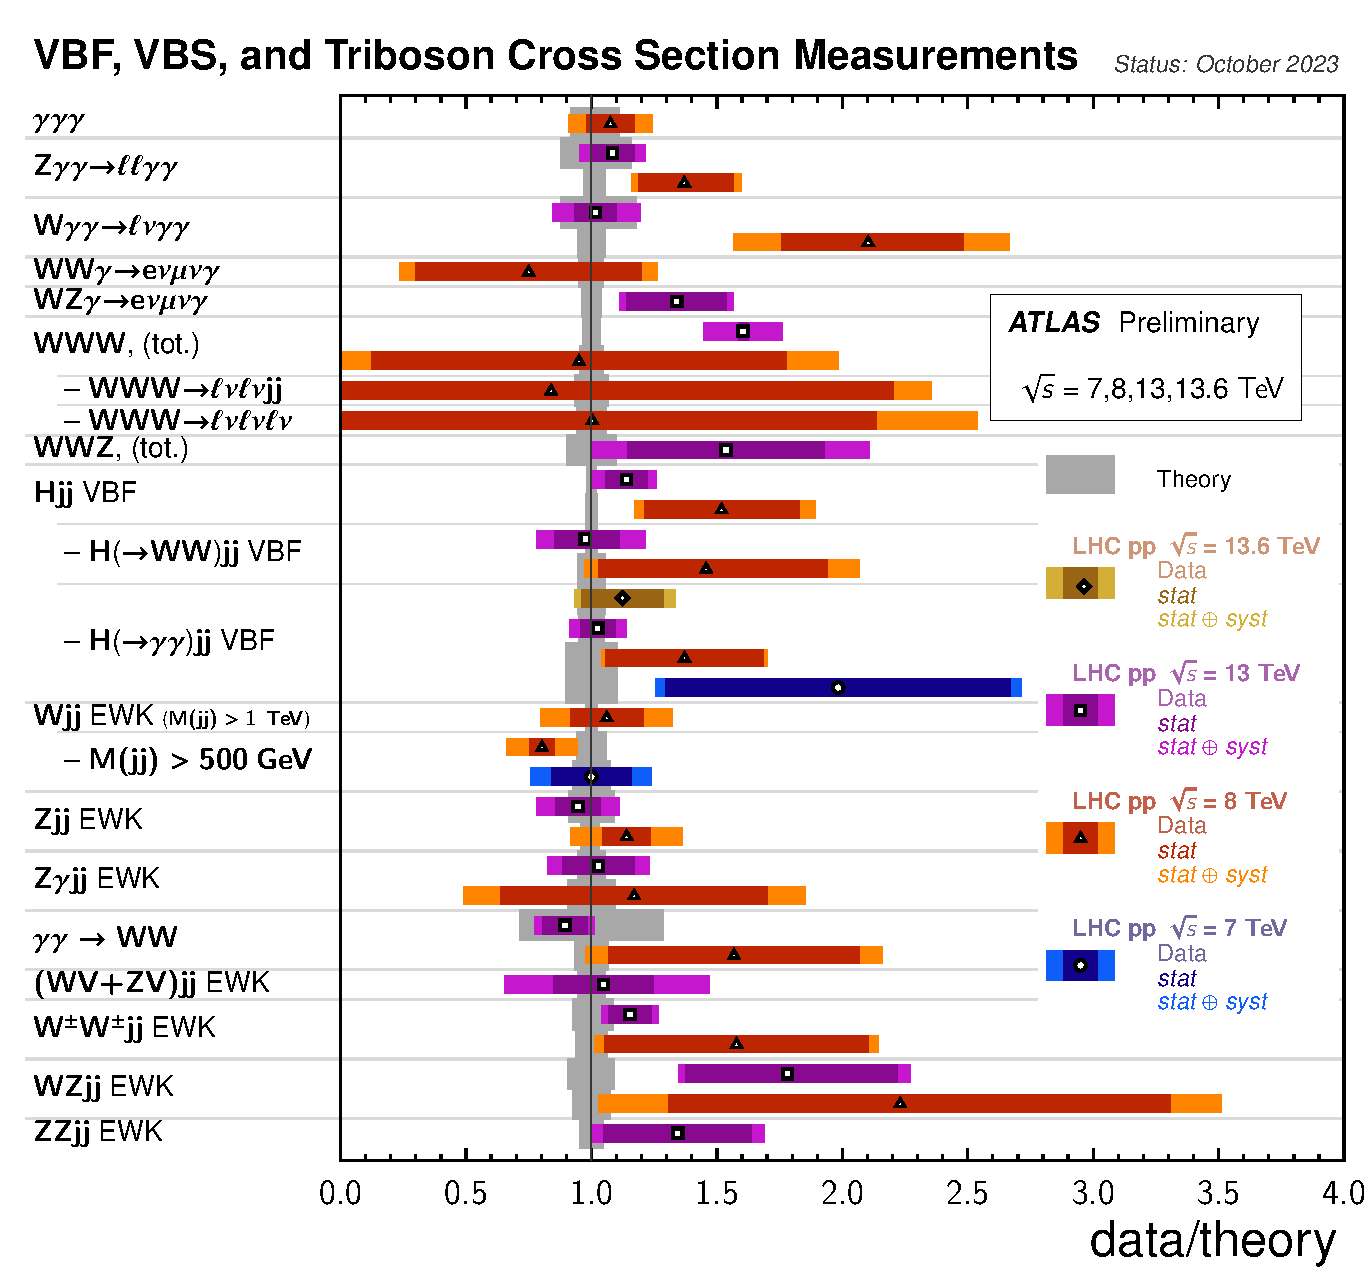
\includegraphics[width=\textwidth]{plots/theory/SM_VBS_Measurements.pdf}
    \caption{Overview data-to-theory ratios for a selection of ATLAS cross-section measurements for VBS, VBF, and triboson production. Measurements of these processes gives rise to an increasingly large body of constraints to quartic electroweak interactions. Figure from \cite{Theory:AtlasSummary}.\label{fig:smvbsmeasurements}}
\end{figure}

% Next status of VBS measurements and observations, and why background large, reword beginning a little bit

%Why backgrounds so much larger? Why large separation, tag jets etc.

% NEW SECTION -- VBS
% What is VBS? Why is it interesting? The Higgs divergence thing is of historical interest, can mention it but don't go into too much detail. Feynman diagrams, explain what's going in them and specifically using wyjj as an example and show the Wyjj (forward reference) diagrams to explain this. Then need a statement on what the backgrounds are [for wyjj I guess] and explain why the backgrounds are so much larger. Then describe the status of VBS measurements and observations at the LHC [can show the public cross-sections plot here if you want]. In general explain why VBS-weak boson self interactions are interesting. [A nice example from VBF higgs to show why the tagging jets appear: https://arxiv.org/pdf/1610.08420.pdf page 6]

%Something very quick about phase-space integrals (1-2 lines). Some 1-2 lines about differential cross-sections. Look for a bit to see if you can find an explicit example relating the VBS/VBF. Then go to PDFs

% Something about quanitising the above to get creation and annihilation operators -- still not sure if I actually needed to show the above. What are the states of the free hamiltonian, introduce free and interacting hamiltonian, interaction picture, time evolution operator.

%Plane wave solutions to the KG equation. After quantising can write scalar field operator in terms of anihilation and creation operators. Probability of a transition from state i to state j is given by PCP-2.109. Calculate inner product by S-matrix element.
% S-matrix element (or just matrix element) is the inner product of two states at times +/- infinity where the state at -infinity is evolved to +infinity by the operator S-operator in the interaction picture. David tong p54. PCP has a good discussion of this as well as QFT notes on page 62. [To calculate matrix element to first order, write initial and final states as anihilation and creation operators acting on the vacuum state, expand Shat in terms of powers of g (to first order), write the fields in terms of their creation and anihilation operators then use the ETCR to evaluate vevs of anihilation and creation operators]. We define the AMPLITUDE using equation (2.116, page57) of PCP (actually page 98 of QFT notes better). Can relate matrix elements to greens functions according to equation (18) -- qftmatrixtogreenfunctions.pdf handout -- where the green functions are the time-ordered vevs of fields with an shat operator. Then we can expand s-hat in terms of the interaction hamiltonian (page 80 of QFT notes) up to a given order. Can use wicks theorem to evaluate contractions etc, each contraction is a feynman propagator (scalar yukawa theory). Matrix elements can be represented by feynman diagrams using the feynman rules and where each distinct numerical contributions to a green's function corresponds toa single distinct feynman diagram. (FDs describe MEs not greens functions, AFIK the greens functions give the internal legs and vertices.. but it is still true that each contribution to a greens function has a single distinct feynman diagram -- double check definition of FDs with other sources). PCP - each feynman diagran is a precise mathematical contribution to the amplitude. From FD - xsections: 
% Go back to PCP-2.109, motivate the equation PCP-2.120 eventually giving 2.125-2.126. 

% 1. First subsection on scattering amplitudes and cross-sections. Relate scattering amplitudes to feynman diagrams and feynman diagrams to cross-sections. What is the partonic cross-section model. The thing that's calculable in perturbation theory. Start off with partonic cross-sections. Define interactions that lead you to cross-section. 
% 2. Bring in PDFs. These allow us to calculate cross-sections for processes in pp collisions. Then talk about how partons in final state will form hadronic systems -- The parton shower is/are an approximation to this. Perturbation theory is used, typically at NLO accuracy, sometimes only leading order. 
% 3. Hadronisation part (call this ``formation of hadronic final states'') -- ``catch-22 situation'' Andy suggested looking at how others resolve this...  Concept of PS is more a MC method. Parton shower -- [describes the?] dominant physics process. The ME diverges at small angles, this is the origin of parton shower. Not too many details on how hadronisation works. Should describe how to get from collisions to a stream of partons to hadrons. Should describe the divergence in the matrix element -- high virtuality -- [makes the final states?] likely to split into multiple partons.
% 4. Subsection on MC. (around 2 pages?) Partonic cross-section calculation at NLO using: [multiplicity??] merging, parton shower and hadronisation algorithms, underlying event and MPI. Then discuss what the state of the art in simulation is. Should discuss PS and hadronisation as a concept [I guess in the previous subsection] and then here go into the algorithms for the PS and hadronisation models e.g. PT ordering/angular ordering in pythia/herwig etc. 


%have an idential yukawa term as for leptons. eqn 4.6.17 with masses given by y_{u/d}v/sqrt(2). Here, just like in equation 2.46, we have assumed there are only diagonal yukawa terms, i.e. we don't have terms like y(l1phil2) [or can write q here]. However, in reality the matrix of yukawa terms only becomes diagonal by redifining the (lepton/) quark fields using  (eq 4.6.16), in this way V_6daggerYV is diagonal (this is called singular value decomposition). This rotation effects the kinetic term because left and right handed quark fields are rotated differently  resulting in terms like (eq 4.6.12), which implies that the weak interaction can change the quark family. This is summarised by the CKM matrix (eq 4.6.19). SSB gives rise to the quark mass terms, where the masses are given by (4.6.21). Finally can write down SM lagrangian.

%Now can have this bit in this section:  
%The SM has SU(3)xSU(2)xU(1) gauge symmetry, where the SU(3) gauge fields are given by G_munu. The residual symmetry group of the SM is SU(3)xU(1) (where the residual U(1) symmetry is actually a linear combination of original U(1) and a subgroup of SU(2)), meaning that SU(3) is not a broken gauge symmetry hence the G gauge fields do not gain mass under the higgs mechanism. Only a kinetic term for the G gauge fields. Therefore the covariant derivative term can be written like this: equation 4.5.1, where Y is the U(1) ``hypercharge'' which is just a real coefficient which changes depending on how a particular field transforms under U(1). The theory also contains a left-handed lepton field which has zero ``charge'' under SU(3) as leptons do not interact with the strong force and is doublet (for electron and neutrinos) (Write this down in the notation with three indices for the three different families). Since the weak force can change electrons into neutrinos they should be charged under SU(2) and since these are doublets they should tranform under the 2x2 matrices which make up the ``fundamental representation'' of SU(2) (rather than a different reducible representatoin which is not necessarily 2x2 matrices). We want the higgs field to be of the form discussed in the previous section, hence the hypercharge is 1/2 and should have SU(3) charge of zero. The theory also contains a one-component right handed spinor field which is neutral (uncharged) under SU(3) and SU(2). Go over charge operator and why hypercharges have to be -1/2 and -1. Mass term like equation (4.5.9) is not allowed, therefore write it like (4.5.10) and now this is invariant under SU(2) and U(1). After SSB becomes (4.5.17) and the left and right handed spinors have combined to become the physical electrically charged lepton fields. No mass term for neutrinos. Masses are given by ml^f = y_l^fv/sqrt(2). 


% Note to self: Probs too much info, but the A_mu gauge field components here are in the T-hat basis, so the eigenvectors of the S_ab matrix give the combinations of the A_mu in the original basis, the components of these eigenvectors are the cos and sin weinberg angles. Also for the W boson we can express these as 1/sqrt(2)(A^2\pmiA^3) because in the quadratic part of the lagrangian we have 0.5Amu^2Amu^2 + 0.5Amu^2Amu^3 + ... but this is equivalent to 1/2(amu^2\mp iamu^3)(amu^2\pm iamu3) which can then be identified as the W boson fields. So, tldr - what I wrote above is correct. 
%\begin{equation}
%    
%\end{equation}
% To realise the lagrangian for the unified electroweak theory, have to introduce the concept of local non-abelian gauge transformations, in this case a scalar field transforms as phi->matrix phi, and vector field as A-> MAMdagger + ... . The special unitary group SU(N ), defined as the group of complex N × N matrices with M † M = 1 and det M = 1. Number of basis matrices -- generators -- given by D = N^2-1 (U(1) is D=N^2)``dimensionality of the group''. Non-abelian local gauge transformations can be realised if the gauge field can be written as a linear combination of the generators of the group (representation). (we say the gauge field is an element of the algebra). This means the gauge fuield can be written as a D component vector field. Write A^mu in terms of generators. Using this notation, it is useful to define the matrix Sab. Can show that the unbroken generators are giben by eigenvectors of Sab with zero eigenvalue. The eigenvectors of Sab can be used to define a new set of generators ordered such that the broken generators come first. (since the unbroken generators leave the vev unchanged, these generate the ``residual symmetry group''). 
% The most general lagrangian in scalar field theory is dmuphidmuphi - potential, dmuphidmuphi is the kinetic term. The kinetic term for the gauge field lagrangian (fmunufmunu) is not gauge invariant in the non-abelian case. However, can show that the TRACE is invariant. Therefore can write down a lagrangian invariant under local U(1) and (non-abelian) SU(2) transformations as [Lagrangian on page for of SM_mccullough], where for the kinetic term of the scalar field, we have covariant derivatives since we have gauged the symmetry (since lagrangian invariant under LOCAL gauge transformations). Now can go into EW unification.
% Consider lagrangian EW unification lagrangian from mccullough (where Amu = Amu^at^a), this has SU2 x U1 symmtery. dimensionality of SU2 is three, therefore there are three SU2 gauge fields (A_mu^a), U(1) has dimensionality one therefore one U(1) gauge field, B_mu. Now, rewrite covariant derivative as in (3.7.4), now can write (Dmuphi)_i as equation 3.6.2, where phi^hat = blablabla. Using that fact phihatphihat = lambda^Bdelta_ab (equation 3.6.4), can write the covariant derivative term as equation (3.6.5) (to quadratic order). Cannot identify mass because of the mixing term. Can remove this mixing term through a gauge choice -- unitary gauge -- which is defined by (equation 3.6.12 with mij replace with 2lambda v^2). Mass of the scalar particle is sqrt(2lambda) v and the eigenvalues of the S matrix give the masses of the vector particles. Now write down Sab as equation (3.7.6), introduce weinberg angles etc, use the pauli matrices and give the eigenvalues and therefore that masses of the photon, W+- and the Z.  
%Only considered Abelian case thus far. (higgs vev 246 GeV)

% adding interaction term is equivalent to ``gauging the symmetry, which is replacing derivatives with covariant derivatives turning the global u(1) symmetry into a local symmetry. ''
%%%%%%%%%%%%%%%%%
%* Say a little bit about local symmetries, (gauging the symmerty?).
%* Motivation (no quite a derivation) of Maxwell lagrangian describing the (massless) photon as a (spin-1) vector field which reproduces all of Maxwell's equations but with zero charge(density) and no current(density) term. Gauge transformations: different vector and scalar potentials give rise to the same electric and magnetic field, so we are free to impose invariance under these transformations. Maxwell Lagrangian Doesn't describe interactions, doesn't describe electrons.Amu = (A,phi). EoM give spatial components satisfy massless Klein-Gordon equation after choosing the ``radiation gauge''. Gauge invariance gives masslessness of photon 
%* Have talk about noninteracting photons, for description of electrons discuss Dirac equation, spinors, spin, etc. Dirac lagrangian. Global U(1) symmetry gives rise to the conserved noether current $j^mu$. Mention Noethers theory says that symmetries give rise to conserved currents. After the spinors are quantised, this leads to a conserved noether charge of PS9[3.113] (page62) which gives the number operators for particle and antiparticles with charge -e. Dont even need to mention raising and lowering operators, just use number operator. Next, gauging the symmetry gives rise to interactions between photons and electrons. Then have the full QED |Lagrangian. 
%Spinors tranform differently than vectors under lorentz transformations

%describes a fixed number of particles %the state of the system is described by a wave function $\psi(x)$.
%\begin{equation}
%    \langle\psi,\phi\rangle=\int\mathrm{d}^3x\psi^*(\underline{x}\phi(\underline{x}))
%\end{equation}
%QM describes a fixed number of particles (or a single particle).
%The basic structure of QM persists to all generalisations such as QFT, string theory, ... No evidence against the basic mathematical structure of QM. 
%QM assumes the universe is split into quantum and classical regimes (unsatifactory)
%
%
%Introduce Theory
%
%\section{QFT and the Standard Model}
%\subsection{Classical Field Theory}
%* Scalar and Vector Fields \\
%* The Maxwell Lagrangian \\
%\subsection{Symmetries in Field Theory}
%* Abelian and non-Abelian Symmetries \\
%* Symmetry groups and Lie Algebras \\
%* Noether's theorem \\
%* Non-Abelian Gauge Fields \\
%* Spontaneous Symmetry Breaking \\
%* (non-Abelian) Higgs Mechanism \\
%* EW Symmetry Breaking \\
%\subsection{Fermions}
%* Dirac Equation \\
%* Dirac Lagrangian \\
%* Leptons \\
%* Quarks \\
%\subsection{The Standard Model}
%\subsection{Calculation of Cross Sections}
%* Phase space integrals \\
%* Example in QED \\
%\subsection{Effective Field Theories}
%\section{Collider Phenomenology and MC generators}
%\subsection{Basics of non-perturbative QCD}
%* Infrared, collinear divergences, IRC safety \\
%* IR limits and ME factorisation \\
%* parton showers, hadronisation, different hadronisation models  \\
%* Resummation  \\
%* Deep inelastic scattering, PDFs \\
%\subsection{Jet Clustering and Jet Substructure}\label{sec:theory:jet}
%* Jet Algorithms \\
%* Cone Algorithms \\
%* Sequential Recombination Algorithms \\
%* Jet Input Objects and Jet Tagging \\
%\subsection{Event Generators}
%* Basics of Monte Carlo methods \\
%* Non-perturbative QCD in MC generators \\
%* Multi-parton interactions, pile-up \\
%* Overview of different MC generators (e.g MG5 vs Powheg vs Sherpa), differences between them, assumptions made \\
%\section{Physics of Vector Boson Scattering/Fusion}
%* Typical event topology and relation to colour flow \\
%* Typical observables characterising VBS/VBF processes \\
%* EFTs and sensitivity to Dim-6 and Dim-8 operators \\
%* CP-odd observables
%
\FloatBarrier
%-------------------------------------------------------------------------

%-------------------------------------------------------------------------
%\newpage
%\chapter{The Large Hadron Collider}
%%* Overview of LHC and experiments at the interaction points
The Large Hadron Collider \cite{LHC:LHC} (LHC) is a two-ring proton-proton and Pb-Pb ion collider installed into the 27km long LEP tunnel at CERN. The primary discovery goal of the LHC was the observation of the Higgs boson which was achieved in July 2012 \cite{Atlas:higgs}. The LHC has two high-luminosity experiments, ATLAS \cite{Atlas:design} and CMS \cite{LHC:CMS} with a design peak luminosity of $10^{34}\text{cm}^{-2}\text{s}^{-1}$, in addition to TOTEM \cite{LHC:TOTEM}, LHCb \cite{LHC:LHCb}, and ALICE \cite{LHC:ALICE}. 

%showing the different beam Insertion Regions (IR) corresponding to 
The proton source for the LHC is a bottle of hydrogen gas. The hydrogen is ionised by an electric field before they are accelerated to around 50\MeV by Linac 2. The Proton Synchrotron (PS) PS accelerates protons to 25\GeV and provides them as bunches with a 25ns spacing to the Super Proton Synchrotron (SPS). The SPS accelerates the bunches to an energy of 450\GeV. The acceleration of proton bunches in the LHC itself is achieved through the radiofrequency (RF) system. The RF system is comprised of 16 RF cavities housed in 4 cryomodules. Each RF cavity delivers an oscillating longitudinal electric field of 5MV/m, delivering an accelerating voltage of 2MV at a frequency of 400MHz. The RF cavities serve two primary purposes, first to accelerate the protons with every pass of the RF system, and second to group the packets of  protons from the PS into even tighter bunches, to ensure a high luminosity at the collision points. The proton injection is timed such that the center of a packet of protons is located just after the oscillating field maximum. Hence, protons just before the center of the bunch (closer to the field maximum) will be accelerated more than protons just after the center of the bunch (further from the field maximum). This results in protons away from the center of the bunch to be moved towards the center, creating stable, tight, bunches. The number of possible stable bunches ($h$) is therefore equal to the number of possible synchronised protons. A proton is synchronised if the RF frequency ($f_{\text{RF}}$) is an integer multiple of the revolution frequency ($f_{\text{rev}}$)
\begin{equation}
    f_{\text{RF}}=h\times f_{\text{rev}}.
\end{equation}
Therefore dividing the two frequencies gives the number of possible bunches. With $f_{\text{rev}}=c/27$km and $f_{\text{RF}}=400$MHz, this gives the value of $h$ as approximately 35640. These are called RF buckets. Not every RF bucket is filled, and the number of occupied buckets in the LHC is 2808. Each bunch contains $\sim \num{1.15e11}$ protons \cite{LHC:design,LHC:acceleratorspedestrians,LHC:rfcavities}. A schematic of the CERN accelerator complex is shown in Figure \ref{fig:LHC:ccc}.
\begin{figure}[t]
    \centering
    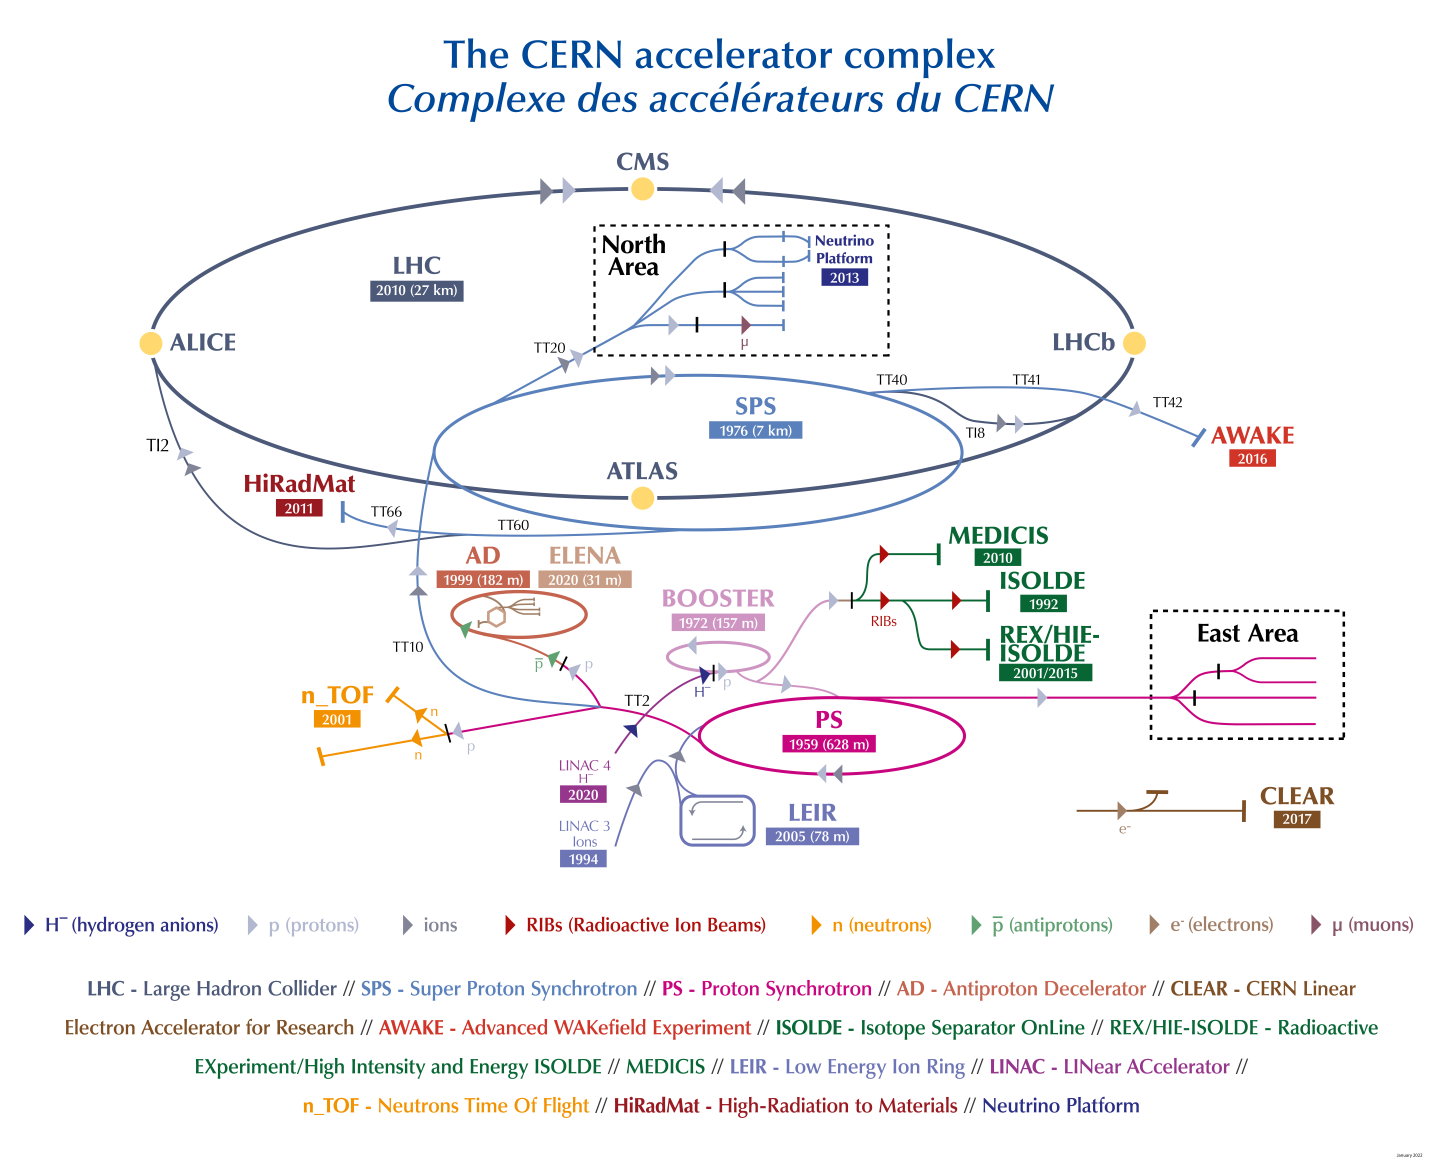
\includegraphics[width=\textwidth]{plots/lhc/CCC-v2022.png}
    \caption{The CERN accelerator complex. Figure taken from \cite{LHC:CCC}.\label{fig:LHC:ccc}}
\end{figure}
As protons carry electric charge, the particle beam will naturally diverge. In the curved sections of the LHC (arcs), the beam must be focused such that its width and height are constrained to be within the vacuum chamber. At the interaction Points (IPs), to enhance the interaction probability for each bunch crossing, the beams are focussed to a size of 16$\mu$m in the $x-y$ plane for CMS and ATLAS. The focussing in the arcs is achieved by collections of superconducting quadrupole, dipole, and other multipole magnets organised into twenty-three LHC cells per arc, resulting in a total of 858 quadrupoles and 1232 dipoles. For the 1232 superconducting dipoles to operate reliably at the 8.33T magnetic field required for 7 TeV beams, the magnet system must operate in a bath of superfluid helium at a temperature of 1.9K. Dispersion suppressors, comprised of four quadrupoles separated by two dipole magnets, are located at the boundaries between the beam insertion regions (IRs) and the arcs, and reduce the machine dispersion (momentum spread of particles within a bunch). Reducing the machine dispersion at the IPs to zero requires two additional quadrupole magnets at each side of the arc. The focusing of the bunches at the IP is achieved using 8 sets of superconducting ``inner triplet'' magnets \cite{LHC:magnets1,LHC:magnets2,LHC:design}. 
%
%\begin{figure}[htb]
%    \centering
%    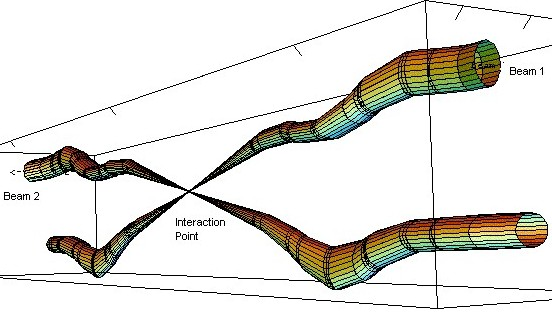
\includegraphics[width=0.6\textwidth]{plots/lhc/interactionpoint_lhc.jpg}
%    \caption{The geometrical configuration of beams leading up to the IPs at the LHC. Figure from \cite{LHC:beams}}
%    \label{fig:lhc_ip}
%\end{figure}
%Before protons reach the LHC, they are accelerated through the LHC injection chain which is comprised of the Proton Synchrotron (PS) and Super Proton Synchrotron (SPS). The PS accelerates protons to 25\GeV and provides them as packets with a 25ns spacing to the SPS. The SPS then accelerates the packets to an energy of 450\GeV. The acceleration of proton packets in the LHC itself is achieved through the radiofrequency (RF) system. The RF system is comprised of 16 RF cavities housed in 4 cryomodules located in LSS4 of the LHC ring. Each RF cavity delivers an oscillating longitudinal electric field of 5MV/m delivering an accelerating voltage of 2MV at a frequency of 400MHz. The RF cavities serve two primary purposes, first to accelerate the protons with every pass of the RF system, and second to group the packets of  protons from the PS into even tighter bunches to ensure a high luminosity at the collision points. The grouping into tight bunches happens because the protons tend to oscillate around those synchronised with the RF frequency. The proton injection is timed such that the center of a packet of protons is located just after the oscillating field maximum. Hence protons just before the maximum will accelerate towards the center, and protons after the maximum will decelerate towards the center, creating stable bunches. The number of possible stable bunches ($h$) is therefore equal to the number of possible synchronised protons. A proton is synchronised if the RF frequency is an integer multiple of the revolution frequency:
%\begin{equation}
%    f_{\text{RF}}=h\times f_{\text{rev}},\hspace{5pt} h=\frac{f_{\text{RF}}}{f_{\text{ref}}}.
%\end{equation}
%Substituting the protons revolution frequency of $c/27\text{km}$ and substituting the RF frequency of 400MHz, gives the value of $h\approx35640$, which is number of possible bunches. These are called RF buckets. Not every RF bucket is filled, and the number of occupied buckets in the LHC is 2808 \cite{LHC:design}\cite{LHC:acceleratorspedestrians}\cite{LHC:rfcavities}.
%only see the maximum accelerating voltage at the gap at an interval equal to an integer multiple of the 400MHz electric field frequency, and %Protons are initially injected into the cavities at an energy of 450\GeV after passing through the pre-accelerator known as the Super Proton Synchrotron (SPS). % Since there are 8 RF cavities, with every pass a proton receives 2MV$\times$8=16MeV of energy. Assuming protons travel at the speed of light, and taking the circumference of the LHC ring as 26669m, means that there are 11245 passes per second, resulting in $11245\times16\MeV=0.18\TeV$  %The RF cavities are responsible for bringing the beam energy up to 6.5 TeV (6.8TeV in run3). The frequency of the RF cavities is tuned to around 400MHz, 
%Now include some info about number of bunch crossings/second, number of interactions per second, primary verticles vs pileup vertices, etc.

\clearpage
\section{Luminosity and cross-sections}

The number of scattering events $N$ in a given amount of time is called the event rate, and depends on the geometric nature of the beam, and on the individual $pp$ interactions. For a given bunch crossing, each proton has an associated cross-sectional area where if another proton is within this, they may interact. It follows that the scattering probability is related to a quantity with units of area known as the \textit{scattering cross-section}, $\sigma$. $N$ is directly related to $\sigma$ and must satisfy
\begin{equation}\label{eq:instlumi}
    \frac{\mathrm{d}N}{\mathrm{d}t}=\mathcal{L}(t)\sigma,
\end{equation}
which defines the quantity known as the \textit{instantaneous luminosity} $\mathcal{L}(t)$. Integrating this equation yields the integrated luminosity $L$
\begin{equation}
    L=\int_{0}^{T}\mathcal{L}\mathrm{d}t,
\end{equation}
which is a measure of how much data has been taken in time $T$. Equation \ref{eq:instlumi} can be written in terms of $L$ as \cite{Buckley:PCP}
\begin{equation}
    N=\sigma L.
\end{equation}
The instantaneous luminosity depends on a number of beam parameters, and is given by
\begin{equation} \label{eq:lumi_1}
    \mathcal{L}(t)=\frac{N_b^2n_bf_{rev}\gamma_r}{4\pi\epsilon_n\beta^*},
\end{equation}
where $N_b$ is the number of particles per bunch, $n_b$ the number of bunches per beam, $f_{\text{rev}}$ the revolution frequency, $\gamma_r$ the relativistic gamma factor, $\epsilon_n$ the normalized transverse beam emittance (this reflects the beam quality, and is roughly defined as the smallest opening the beam can be squeezed through), $\beta^*$ the beta function (the width of the beam, squared, divided by the emittance) at the collision point and $F$ a geometric luminosity reduction factor. The linear dependence on $\gamma_r$ and square dependence on $N_b$ implies that a large luminosity requires beams of high energy and high intensity. Separate dipole magnetic fields and vacuum systems are required for the two beams, as both beams contain positively charged protons. At the IRs the two beams share a common 126m (for ATLAS and CMS) long beam pipe.

The luminosity in the LHC is not constant over a physics run. The beam intensities and emittances of the circulating beams degrade primarily due to the collisions themselves, leading to a decay in the luminosity. This is quantified with the luminosity lifetime, $\tau_L$. 

The expected integrated luminosity of the LHC of a luminosity run is given by
\begin{equation}
    L=L_0\tau_L(1-e^{-T_{\text{run}}/\tau_L}),
\end{equation}
where the assumption is made that the time for beam injection, ramping up the beam energy, ramping down the magnets, and programmed main systems checks total a turnaround time of $T_{\text{turnaround}}\approx 70\text{min}$. Assuming that the LHC is taking data 200 days a year for an optimum run time of 12h, the total maximum luminosity per year is about 120\invfb \cite{LHC:design}.

The Run-2 total integrated luminosity is shown in Figure \ref{fig:LHC:intlumi}. The Run-2 integrated luminosity recorded by ATLAS with good data quality is $140.1\infb$ \cite{LHC:atlaslumi}.

\begin{figure}[t]
    \centering
    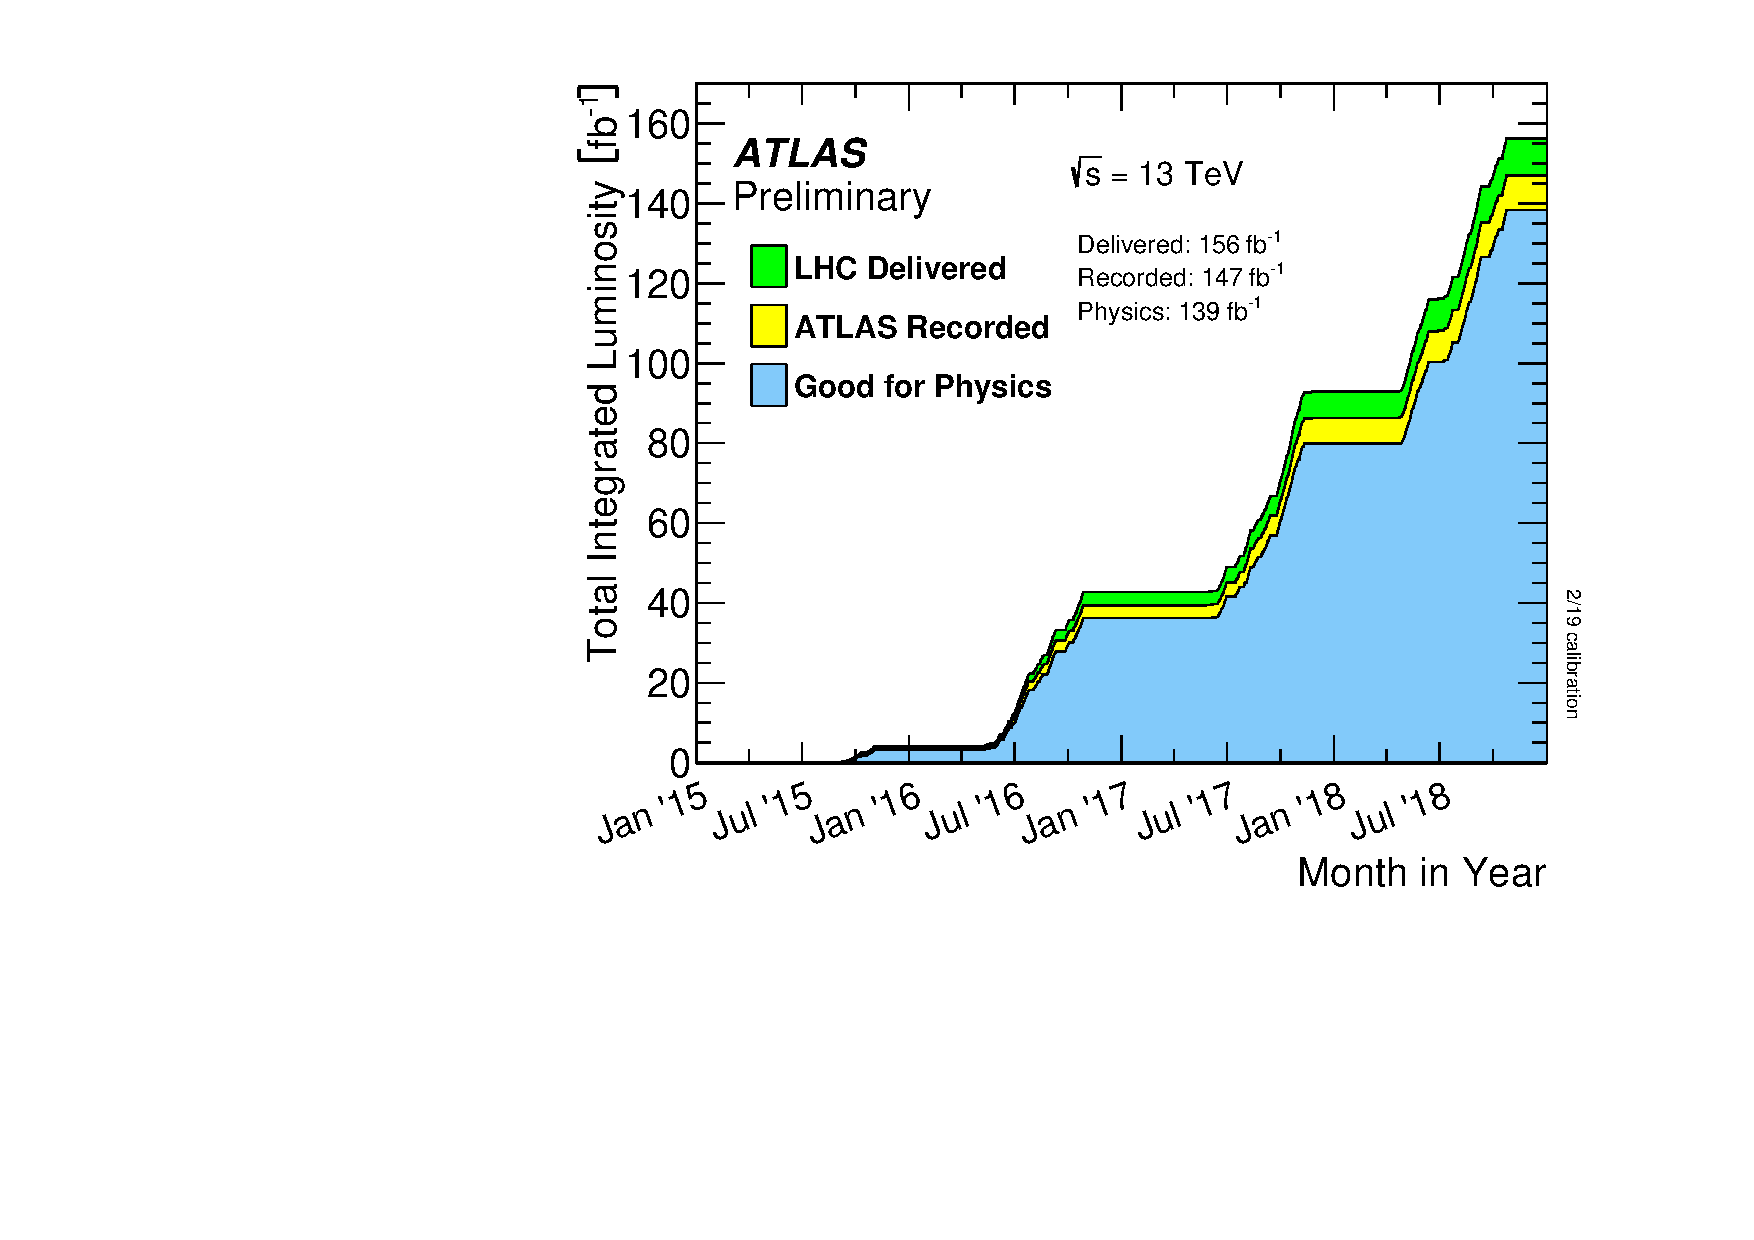
\includegraphics[width=\textwidth]{plots/lhc/intlumivstimeRun2DQall.pdf}
    \caption{The total integrated luminosity for Run-2 versus time. The green curve shows the luminosity delivered to ATLAS by the LHC. The yellow curve shows the luminosity recorded by ATLAS. The blue curve shows the luminosity of the dataset certified to be good data quality. Since this plot has been produced, the most accurate assessment of the total integrated luminosity certified good for physics has been updated to 140\infb \cite{LHC:atlaslumi}. Figure from \cite{LHC:deliveredlumi}.\label{fig:LHC:intlumi}}
\end{figure}

\clearpage
\section{Pile-up}

All LHC analyses need to contend with the harsh experimental conditions which come about due to the very large number of interactions per bunch crossing. The mean number of interactions per bunch-crossing (averaged over luminosity) $\langle\mu\rangle$ in Run-2 was $\langle\mu\rangle = 33.7$. The largest momentum transfer happens in the primary hard scatter interaction, all other secondary interactions are referred to as pile-up interactions and consist mainly of soft-QCD processes. There are two types of pile-up. In-time pileup refers to $pp$ collisions from the same bunch-crossing as the interaction of interest, whereas out-of-time pileup refers to $pp$ collisions occurring in bunch-crossings just before and after the interaction of interest. 

Pileup is responsible for a large number of soft hadrons distributed throughout the detector. Therefore the reconstruction of jets and Missing Transverse Energy (MET) are especially effected. Without pileup mitigation techniques, the energies of jets will in general be overestimated, and spurious jets not associated with the hard scatter will be included in the event leading to changes in the MET measurement. In addition to these biases, pileup also results in the degradation of the resolution of reconstructed quantities. The reason for this is that the pileup activity itself is not a fixed quantity, which therefore results in fluctuations of the bias due to pileup. The challenges associated with pileup in the context of object reconstruction is discussed in more detail in Section \ref{sec:objreco} \cite{Buckley:PCP,LHC:pileup}.

%\label{sec:largehadroncollider}
%\FloatBarrier
%------------------------------------------------------------------------- 

%-------------------------------------------------------------------------
\newpage
\chapter{The LHC and ATLAS Experiment}
\label{sec:atlasdetector}
\section{The Large Hadron Collider}
%* Overview of LHC and experiments at the interaction points
The Large Hadron Collider \cite{LHC:LHC} (LHC) is a two-ring proton-proton and Pb-Pb ion collider installed into the 27km long LEP tunnel at CERN. The primary discovery goal of the LHC was the observation of the Higgs boson which was achieved in July 2012 \cite{Atlas:higgs}. The LHC has two high-luminosity experiments, ATLAS \cite{Atlas:design} and CMS \cite{LHC:CMS} with a design peak luminosity of $10^{34}\text{cm}^{-2}\text{s}^{-1}$, in addition to TOTEM \cite{LHC:TOTEM}, LHCb \cite{LHC:LHCb}, and ALICE \cite{LHC:ALICE}. 

%showing the different beam Insertion Regions (IR) corresponding to 
The proton source for the LHC is a bottle of hydrogen gas. The hydrogen is ionised by an electric field before they are accelerated to around 50\MeV by Linac 2. The Proton Synchrotron (PS) PS accelerates protons to 25\GeV and provides them as bunches with a 25ns spacing to the Super Proton Synchrotron (SPS). The SPS accelerates the bunches to an energy of 450\GeV. The acceleration of proton bunches in the LHC itself is achieved through the radio frequency (RF) system. The RF system is comprised of 16 RF cavities housed in 4 cryomodules. Each RF cavity delivers an oscillating longitudinal electric field of 5MV/m, delivering an accelerating voltage of 2MV at a frequency of 400MHz. The RF cavities serve two primary purposes, first to accelerate the protons with every pass of the RF system, and second to group the packets of  protons from the PS into even tighter bunches, to ensure a high luminosity at the collision points. The proton injection is timed such that the center of a packet of protons is located just after the oscillating field maximum. Hence, protons just before the center of the bunch (closer to the field maximum) will be accelerated more than protons just after the center of the bunch (further from the field maximum). This results in protons away from the center of the bunch to be moved towards the center, creating stable, tight, bunches. The number of possible stable bunches ($h$) is therefore equal to the number of possible synchronised protons. A proton is synchronised if the RF frequency ($f_{\text{RF}}$) is an integer multiple of the revolution frequency ($f_{\text{rev}}$)
\begin{equation}
    f_{\text{RF}}=h\times f_{\text{rev}}.
\end{equation}
Therefore dividing the two frequencies gives the number of possible bunches. With $f_{\text{rev}}=c/27$km and $f_{\text{RF}}=400$MHz, this gives the value of $h$ as approximately 35640. These are called RF buckets. Not every RF bucket is filled, and the number of occupied buckets in the LHC is 2808. Each bunch contains $\sim \num{1.15e11}$ protons \cite{LHC:design,LHC:acceleratorspedestrians,LHC:rfcavities}. A schematic of the CERN accelerator complex is shown in Figure \ref{fig:LHC:ccc}.
\begin{figure}[t]
    \centering
    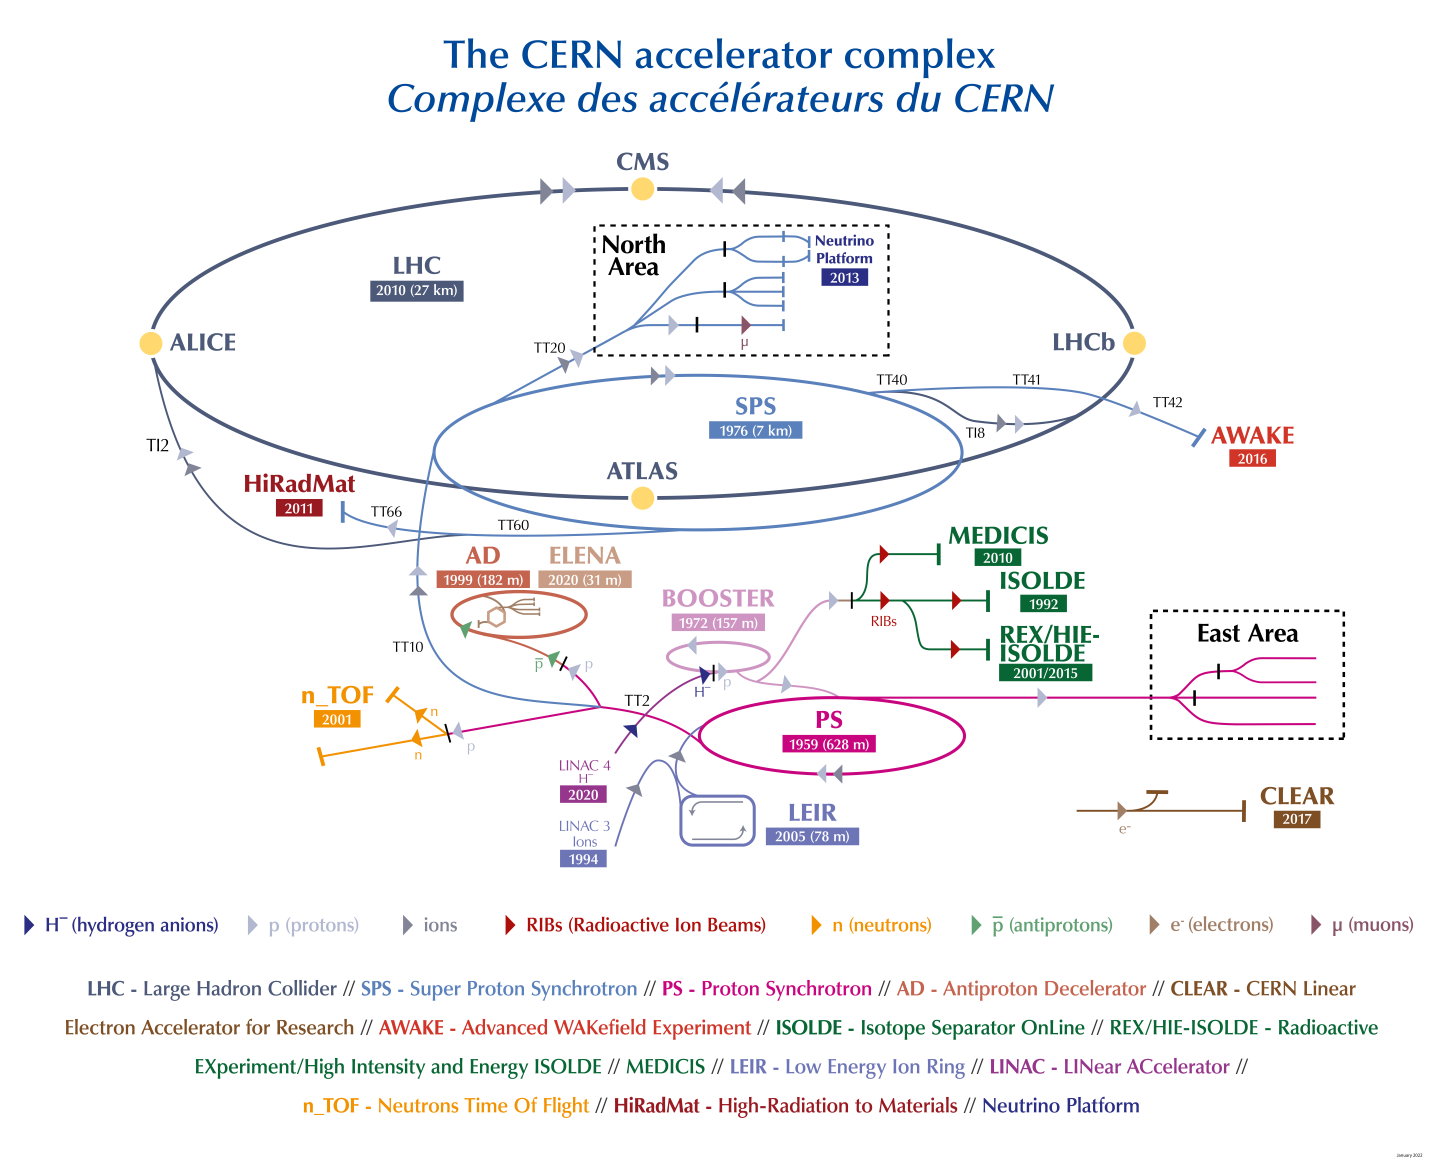
\includegraphics[width=\textwidth]{plots/lhc/CCC-v2022.png}
    \caption{The CERN accelerator complex. Figure taken from \cite{LHC:CCC}.\label{fig:LHC:ccc}}
\end{figure}

As protons carry electric charge, the particle beam will naturally diverge. In the curved sections of the LHC (arcs), the beam must be focused such that its width and height are constrained to be within the vacuum chamber. At the interaction Points (IPs), to enhance the interaction probability for each bunch crossing, the beams are focussed to a size of 16$\mu$m in the $x-y$ plane for CMS and ATLAS. The focussing in the arcs is achieved by collections of superconducting quadrupole, dipole, and other multipole magnets organised into twenty-three LHC cells per arc, resulting in a total of 858 quadrupoles and 1232 dipoles. For the 1232 superconducting dipoles to operate reliably at the 8.33T magnetic field required for 7 TeV beams, the magnet system must operate in a bath of superfluid helium at a temperature of 1.9K. Dispersion suppressors, comprised of four quadrupoles separated by two dipole magnets, are located at the boundaries between the beam insertion regions (IRs) and the arcs, and reduce the machine dispersion (momentum spread of particles within a bunch). Reducing the machine dispersion at the IPs to zero requires two additional quadrupole magnets at each side of the arc. The focusing of the bunches at the IP is achieved using 8 sets of superconducting ``inner triplet'' magnets \cite{LHC:magnets1,LHC:magnets2,LHC:design}. 
%
%\begin{figure}[htb]
%    \centering
%    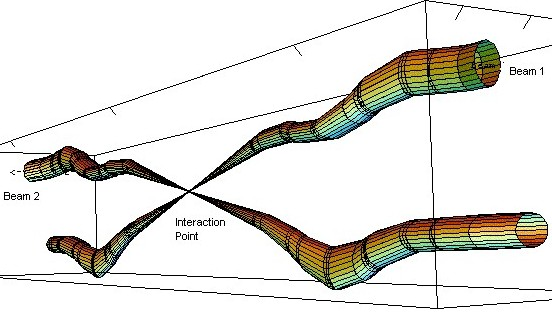
\includegraphics[width=0.6\textwidth]{plots/lhc/interactionpoint_lhc.jpg}
%    \caption{The geometrical configuration of beams leading up to the IPs at the LHC. Figure from \cite{LHC:beams}}
%    \label{fig:lhc_ip}
%\end{figure}
%Before protons reach the LHC, they are accelerated through the LHC injection chain which is comprised of the Proton Synchrotron (PS) and Super Proton Synchrotron (SPS). The PS accelerates protons to 25\GeV and provides them as packets with a 25ns spacing to the SPS. The SPS then accelerates the packets to an energy of 450\GeV. The acceleration of proton packets in the LHC itself is achieved through the radiofrequency (RF) system. The RF system is comprised of 16 RF cavities housed in 4 cryomodules located in LSS4 of the LHC ring. Each RF cavity delivers an oscillating longitudinal electric field of 5MV/m delivering an accelerating voltage of 2MV at a frequency of 400MHz. The RF cavities serve two primary purposes, first to accelerate the protons with every pass of the RF system, and second to group the packets of  protons from the PS into even tighter bunches to ensure a high luminosity at the collision points. The grouping into tight bunches happens because the protons tend to oscillate around those synchronised with the RF frequency. The proton injection is timed such that the center of a packet of protons is located just after the oscillating field maximum. Hence protons just before the maximum will accelerate towards the center, and protons after the maximum will decelerate towards the center, creating stable bunches. The number of possible stable bunches ($h$) is therefore equal to the number of possible synchronised protons. A proton is synchronised if the RF frequency is an integer multiple of the revolution frequency:
%\begin{equation}
%    f_{\text{RF}}=h\times f_{\text{rev}},\hspace{5pt} h=\frac{f_{\text{RF}}}{f_{\text{ref}}}.
%\end{equation}
%Substituting the protons revolution frequency of $c/27\text{km}$ and substituting the RF frequency of 400MHz, gives the value of $h\approx35640$, which is number of possible bunches. These are called RF buckets. Not every RF bucket is filled, and the number of occupied buckets in the LHC is 2808 \cite{LHC:design}\cite{LHC:acceleratorspedestrians}\cite{LHC:rfcavities}.
%only see the maximum accelerating voltage at the gap at an interval equal to an integer multiple of the 400MHz electric field frequency, and %Protons are initially injected into the cavities at an energy of 450\GeV after passing through the pre-accelerator known as the Super Proton Synchrotron (SPS). % Since there are 8 RF cavities, with every pass a proton receives 2MV$\times$8=16MeV of energy. Assuming protons travel at the speed of light, and taking the circumference of the LHC ring as 26669m, means that there are 11245 passes per second, resulting in $11245\times16\MeV=0.18\TeV$  %The RF cavities are responsible for bringing the beam energy up to 6.5 TeV (6.8TeV in run3). The frequency of the RF cavities is tuned to around 400MHz, 
%Now include some info about number of bunch crossings/second, number of interactions per second, primary verticles vs pileup vertices, etc.

\subsection{Detector Luminosity}\label{sec:lumi}

%The number of scattering events $N$ in a given amount of time is called the event rate, and depends on the geometric nature of the beam, and on the individual $pp$ interactions. For a given bunch crossing, each proton has an associated cross-sectional area where if another proton is within this, they may interact. It follows that the scattering probability is related to a quantity with units of area known as the \textit{scattering cross-section}, $\sigma$. $N$ is directly related to $\sigma$ and must satisfy
%\begin{equation}\label{eq:instlumi}
%    \frac{\mathrm{d}N}{\mathrm{d}t}=\mathcal{L}(t)\sigma,
%\end{equation}
%which defines the quantity known as the \textit{instantaneous luminosity} $\mathcal{L}(t)$.
%Integrating Equation \ref{eq:instlumi} yields the integrated luminosity $L$
%\begin{equation}
%    L=\int_{0}^{T}\mathcal{L}\mathrm{d}t,
%\end{equation}
%which is a measure of how much data has been taken in time $T$. Equation \ref{eq:instlumi} can be written in terms of $L$ as \cite{Buckley:PCP}
%\begin{equation}
%    N=\sigma L.
%\end{equation}
The instantaneous luminosity (Equation \ref{eq:instlumi}) depends on a number of beam parameters, and is given by
\begin{equation} \label{eq:lumi_1}
    \mathcal{L}(t)=\frac{N_b^2n_bf_{rev}\gamma_r}{4\pi\epsilon_n\beta^*},
\end{equation}
where $N_b$ is the number of particles per bunch, $n_b$ the number of bunches per beam, $f_{\text{rev}}$ the revolution frequency, $\gamma_r$ the relativistic gamma factor, $\epsilon_n$ the normalized transverse beam emittance (this reflects the beam quality, and is roughly defined as the smallest opening the beam can be squeezed through), $\beta^*$ the beta function (the width of the beam, squared, divided by the emittance) at the collision point and $F$ a geometric luminosity reduction factor. The linear dependence on $\gamma_r$ and square dependence on $N_b$ implies that a large luminosity requires beams of high energy and high intensity. Separate dipole magnetic fields and vacuum systems are required for the two beams, as both beams contain positively charged protons. At the IRs the two beams share a common 126m (for ATLAS and CMS) long beam pipe.

Integrating Equation \ref{eq:instlumi} yields the integrated luminosity $L$
\begin{equation}
    L=\int_{0}^{T}\mathcal{L}\mathrm{d}t,
\end{equation}
which is a measure of how much data has been taken in time $T$. Equation \ref{eq:instlumi} can be written in terms of $L$ as
\begin{equation}
    N=\sigma L.
\end{equation}

The luminosity in the LHC is not constant over a physics run. The beam intensities and emittances of the circulating beams degrade primarily due to the collisions themselves, leading to a decay in the luminosity. This is quantified with the luminosity lifetime, $\tau_L$. 

The expected integrated luminosity of the LHC of a luminosity run is given by
\begin{equation}
    L=L_0\tau_L(1-e^{-T_{\text{run}}/\tau_L}),
\end{equation}
where the assumption is made that the time for beam injection, ramping up the beam energy, ramping down the magnets, and programmed main systems checks total a turnaround time of $T_{\text{turnaround}}\approx 70\text{min}$. Assuming that the LHC is taking data 200 days a year for an optimum run time of 12h, the total maximum luminosity per year is about 120\invfb \cite{LHC:design}.

The Run-2 total integrated luminosity is shown in Figure \ref{fig:LHC:intlumi}. The Run-2 integrated luminosity recorded by ATLAS with good data quality is $140.1\infb$ \cite{LHC:atlaslumi}.

\begin{figure}[t]
    \centering
    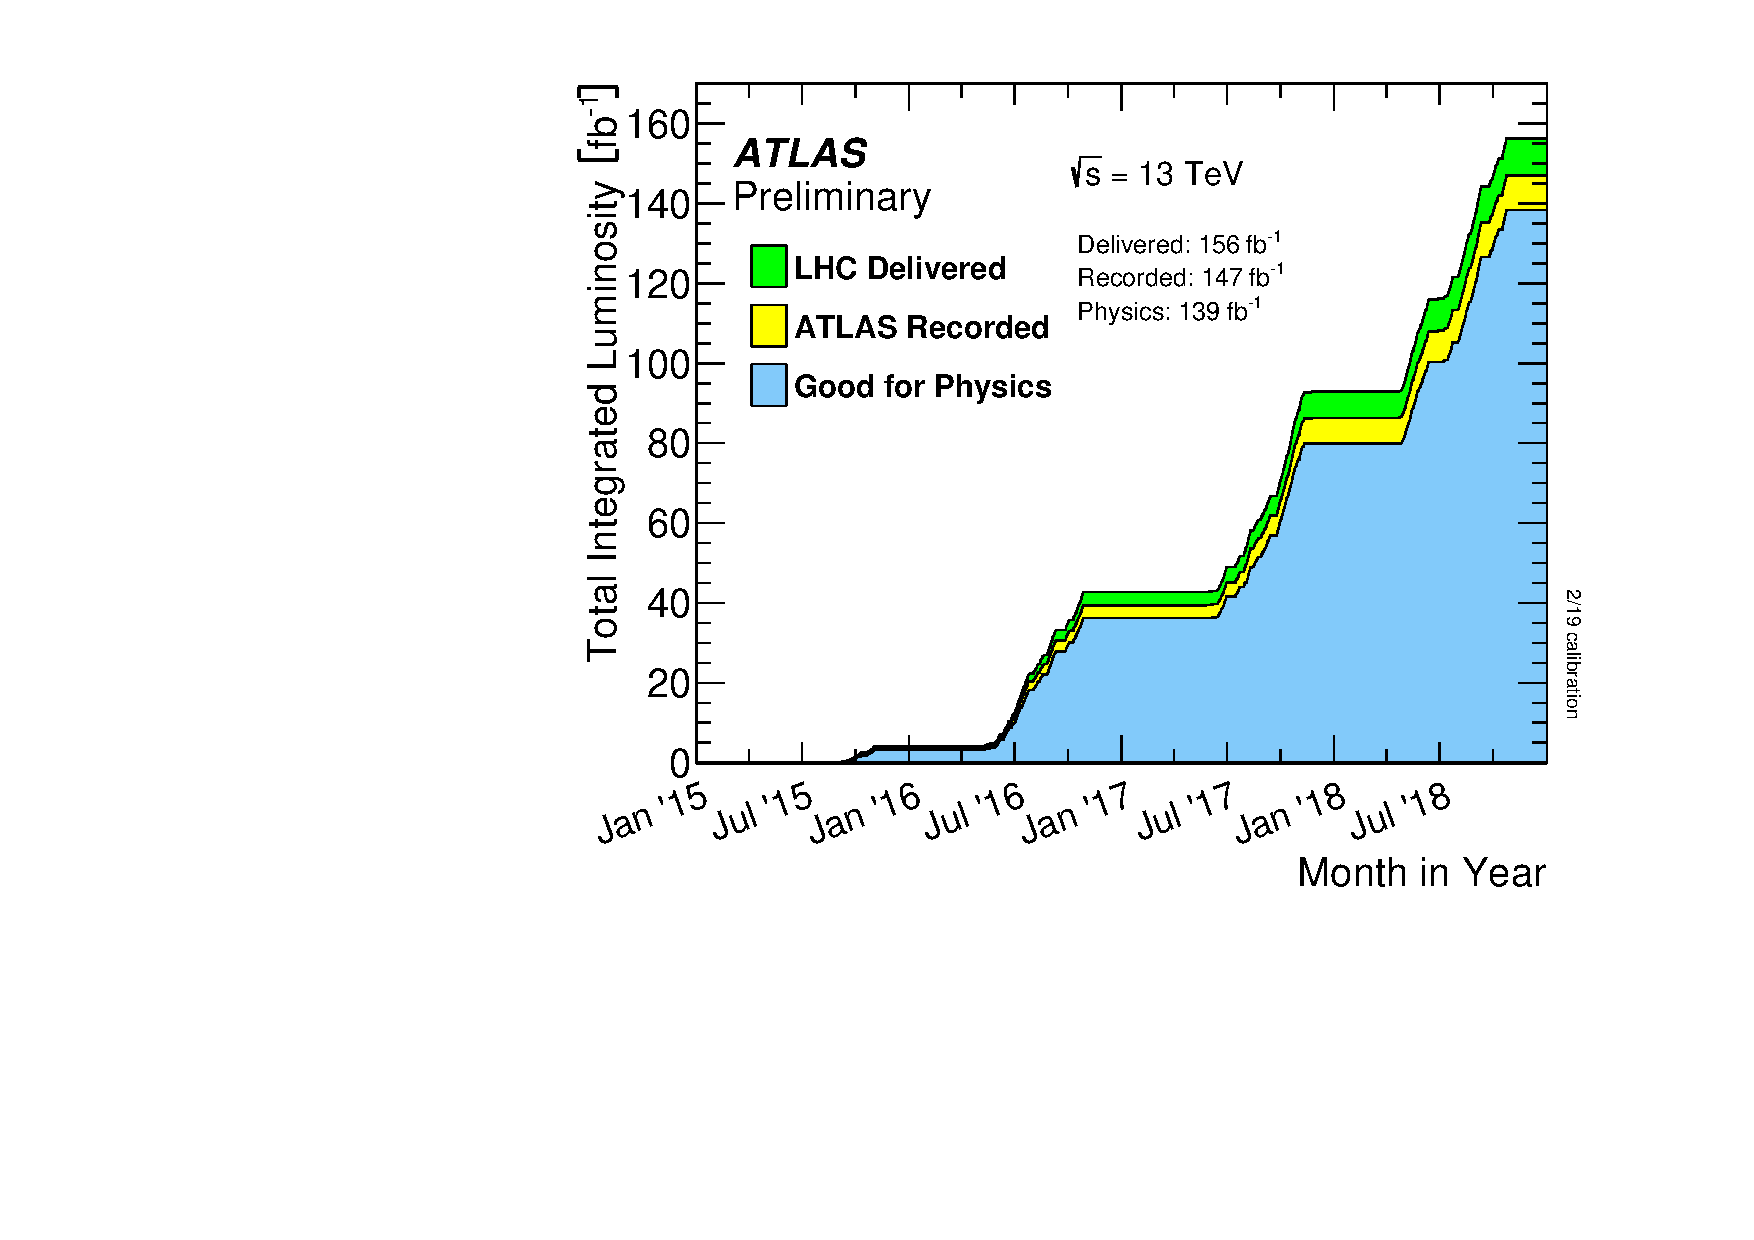
\includegraphics[width=\textwidth]{plots/lhc/intlumivstimeRun2DQall.pdf}
    \caption{The total integrated luminosity for Run-2 versus time. The green curve shows the luminosity delivered to ATLAS by the LHC. The yellow curve shows the luminosity recorded by ATLAS. The blue curve shows the luminosity of the dataset certified to be good data quality. Since this plot has been produced, the most accurate assessment of the total integrated luminosity certified good for physics has been updated to 140\infb \cite{LHC:atlaslumi}. Figure from \cite{LHC:deliveredlumi}.\label{fig:LHC:intlumi}}
\end{figure}

\subsection{Pile-up}

All LHC analyses need to contend with the harsh experimental conditions which come about due to the very large number of interactions per bunch crossing. The mean number of interactions per bunch-crossing (averaged over luminosity) $\langle\mu\rangle$ in Run-2 was $\langle\mu\rangle = 33.7$. The largest momentum transfer happens in the primary hard scatter interaction, all other secondary interactions are referred to as pile-up interactions and consist mainly of soft-QCD processes. There are two types of pile-up. In-time pileup refers to $pp$ collisions from the same bunch-crossing as the interaction of interest, whereas out-of-time pileup refers to $pp$ collisions occurring in bunch-crossings just before and after the interaction of interest. 

Pileup is responsible for a large number of soft hadrons distributed throughout the detector. Therefore the reconstruction of jets and Missing Transverse Energy (MET) are especially effected. Without pileup mitigation techniques, the energies of jets will in general be overestimated, and spurious jets not associated with the hard scatter will be included in the event leading to changes in the MET measurement. In addition to these biases, pileup also results in the degradation of the resolution of reconstructed quantities. The reason for this is that the pileup activity itself is not a fixed quantity, which therefore results in fluctuations of the bias due to pileup. The challenges associated with pileup in the context of object reconstruction is discussed in more detail in Section \ref{sec:objreco} \cite{Buckley:PCP,LHC:pileup}.

\section{The ATLAS Experiment}
The design of the ATLAS detector was initially motivated by the search for the Higgs boson and physics beyond the Standard Model (SM). The challenging experimental conditions at the LHC require fast, radiation-hard electronics and sensors. Large particle fluxes require a good detector granularity. An almost $4\pi$ acceptance is necessary to access the rich physics contained in the forward regions, such as the Vector Boson Scattering (VBS) process targeted in this thesis. Excellent electromagnetic (EM) calorimetry is a requirement for accurate electron and photon identification. The need for accurate jet and MET reconstruction dictates the energy resolution requirements for the hadronic calorimeter systems. Muon identification and momentum resolution must be able to determine the charge of high transverse momentum muons. Finally, a highly efficient trigger and data acquisition system is required to be able to select signal events on interest whilst rejecting backgrounds. 

Figure \ref{fig:atlas_detector} shows the different nested subsystems of the ATLAS detector. From the IP, the products of inelastic p-p collisions travel outwards through the detector subsystems. The origin of the coordinate system is defined as the IP. The beam direction defines the $z$-axis, whereas the $x-y$ plane is transverse to the beam direction. The positive $x$-axis points from the IP to the LHC ring centre, and the positive $y$-axis points upwards. The azimuthal angle $\phi$ is measured around the beam axis; and the polar angle $\theta$ is the angle from the beam axis. The rapidity is defined (in natural units) as
\begin{equation}
y = 1/2\ln [(E+p_z)/(E-p_z)], 
\end{equation}
where $E$ is the energy, and $p_z$ is longitudinal component of the momentum $\mathbf{p}$. In the $|\mathbf{p}|\gg m$ limit, the rapidity can be approximated by the pseudorapidity, $\eta=-\ln\tan (\theta/2)$. The distance between two particles $i$ and $j$ can be quantified using a metric, $\Delta R_{ij}$, which combines the rapidity separation $\Delta y_{ij}\equiv|y_i-y_j|$ and the azimuthal separation $\Delta \phi_{ij}\equiv|\phi_i-\phi_j|$
\begin{equation}
    \Delta R_{ij}=\sqrt{\Delta y_{ij}^2+\Delta\phi_{ij}^2},\hspace{25pt} \Delta R^{\eta}_{ij}=\sqrt{\Delta\eta_{ij}^2+\Delta\phi_{ij}^2}.
\end{equation}
The coordinate system used to describe the kinematics of particles detected at the ATLAS detector is represented schematically in Figure \ref{fig:atlas_coordinates}. The three-momentum of the final-state particle is denoted by $\vec{p}$. The transverse momentum, \pt, is defined by projecting $\vec{p}$ onto the $x-y$ plane and taking the magnitude. %The conservation of momentum in the transverse plane can be exploited due to the hermeticity of the ATLAS detector, and is used to define the missing transverse momentum, $\vec{p}_{T,{\text{miss}}}$, as the negative vector sum of the transverse momenta. The missing transverse energy, $E_T^{\text{miss}}$, or MET is given by the magnitude of $\vec{p}_{T,{\text{miss}}}$.
\begin{figure}[t]
    \centering
    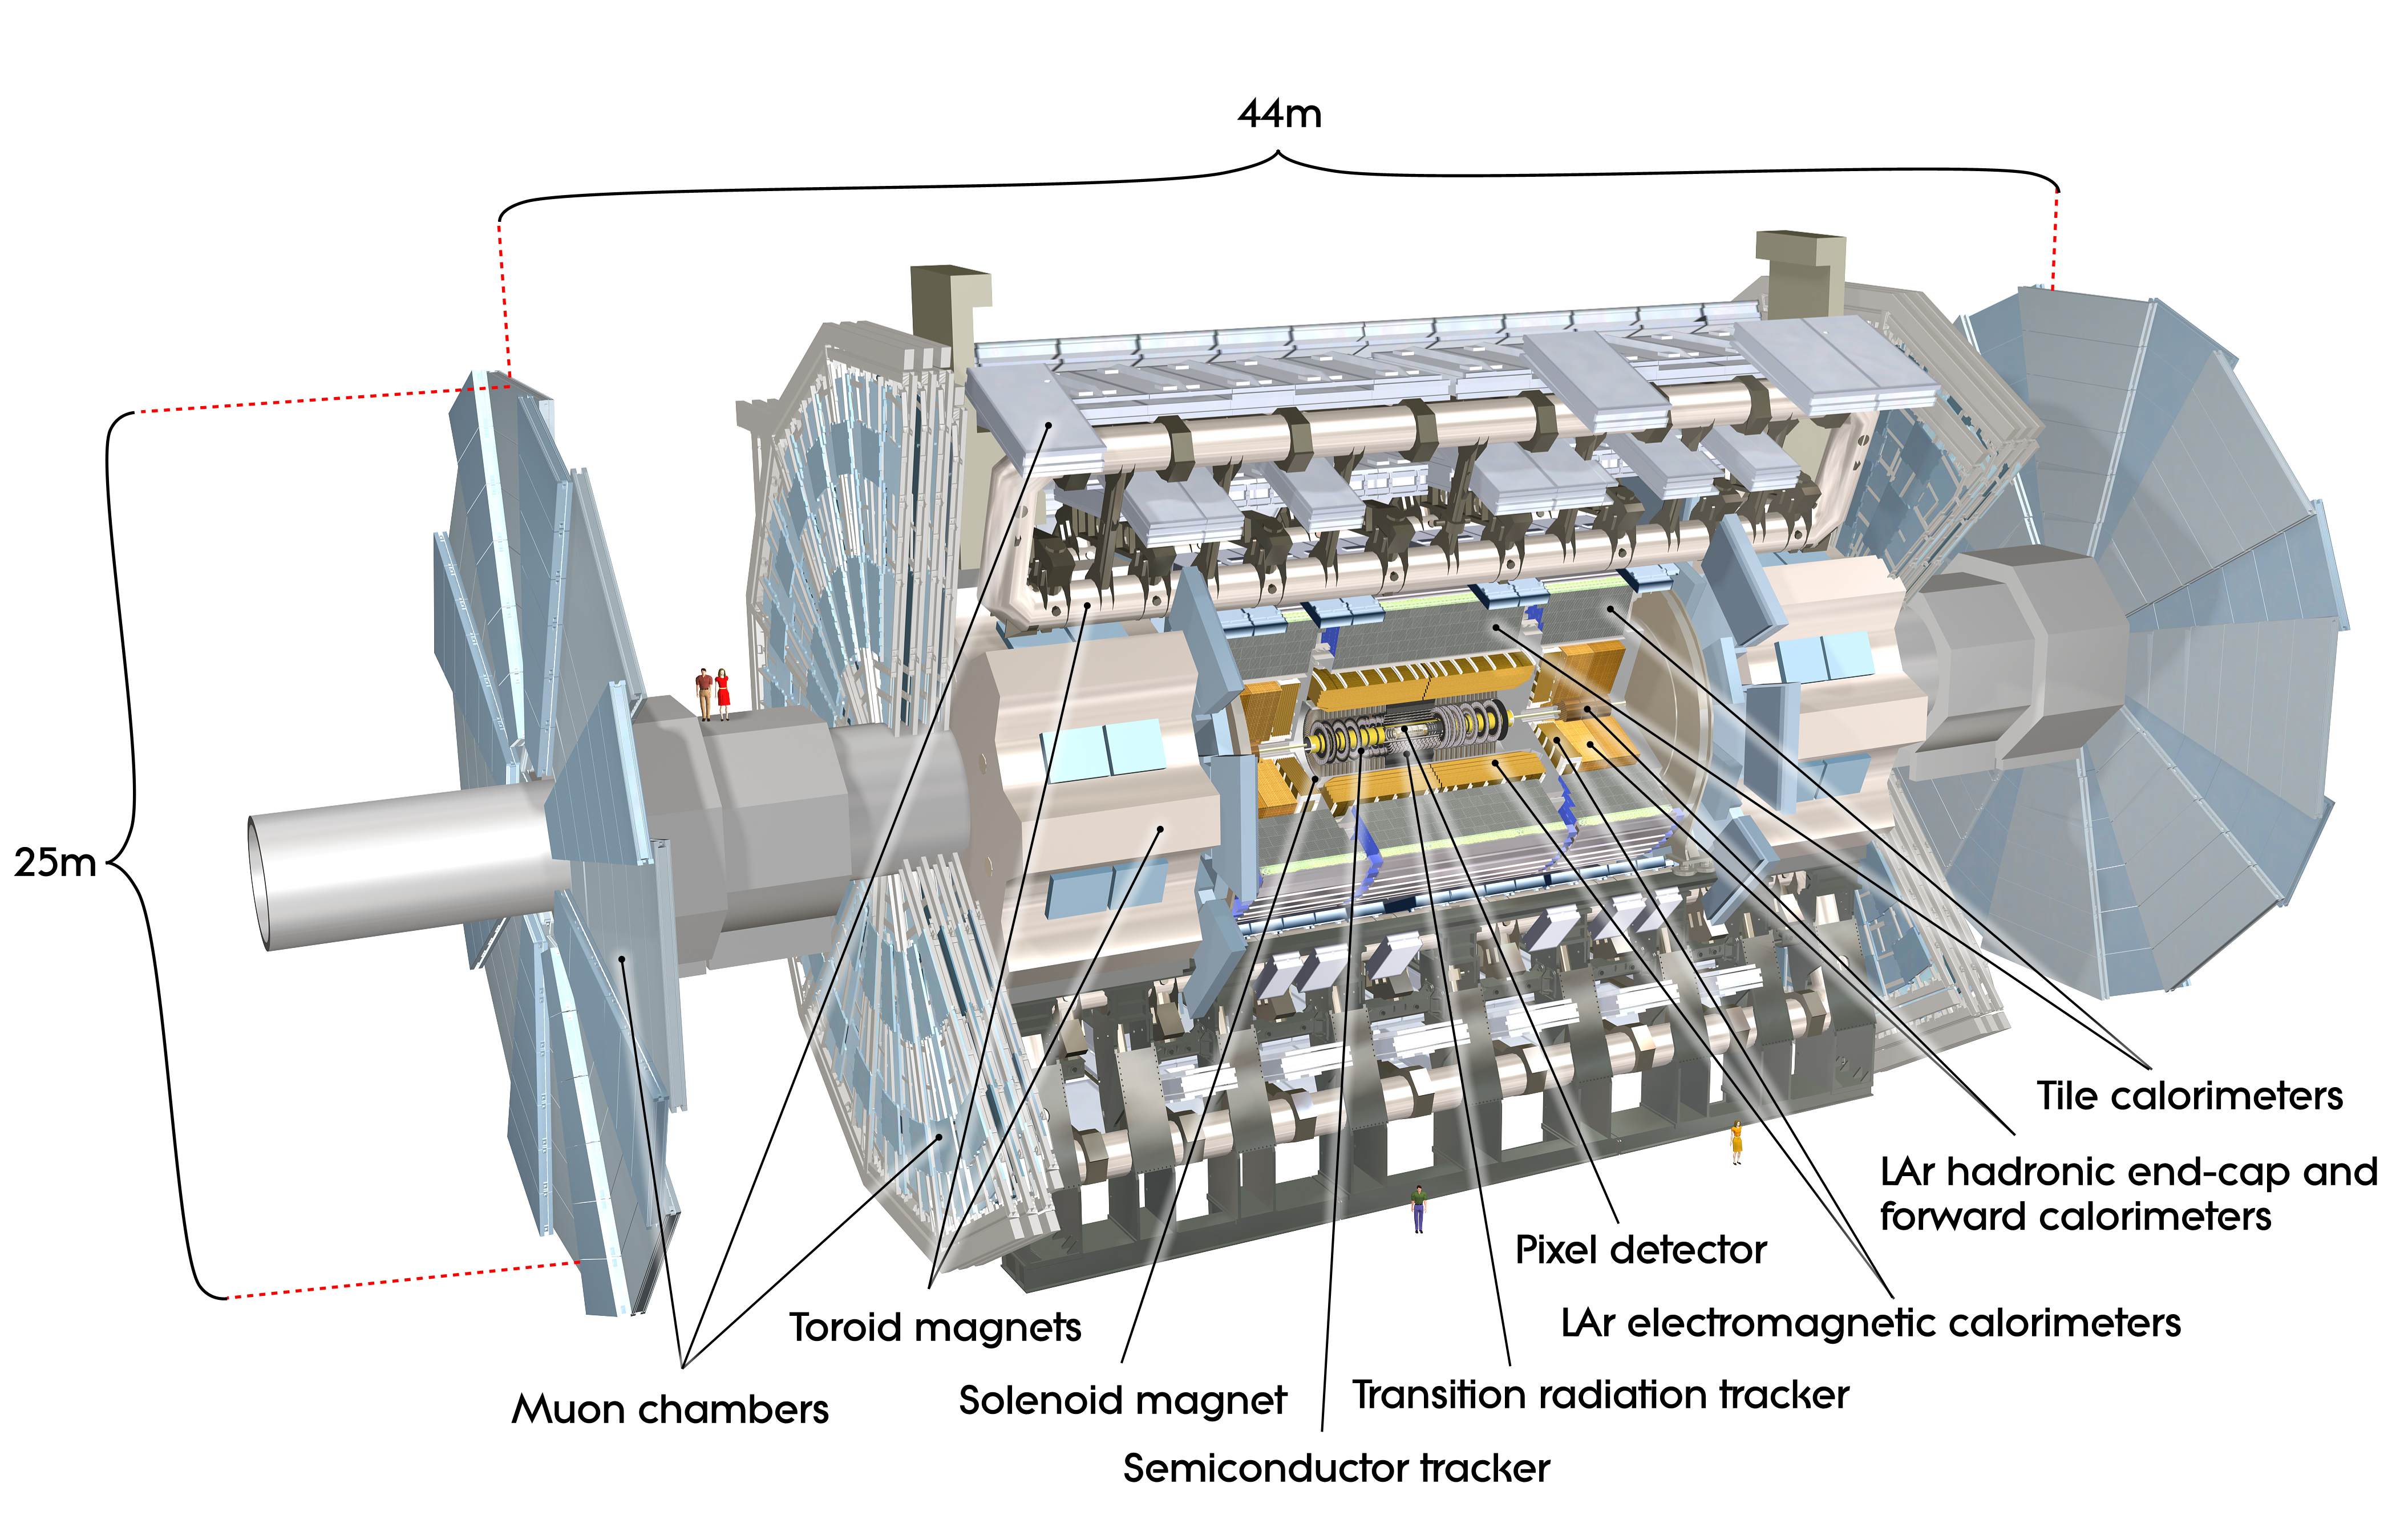
\includegraphics[width=\textwidth]{plots/atlas/ATLAS_Detector.jpg}
    \caption{A cut-out of the ATLAS detector showing the tracking, calorimeter, muon, and magnet systems. Figure from \cite{Atlas:detector}. \label{fig:atlas_detector} }
\end{figure}

\begin{figure}[t]
    \centering
    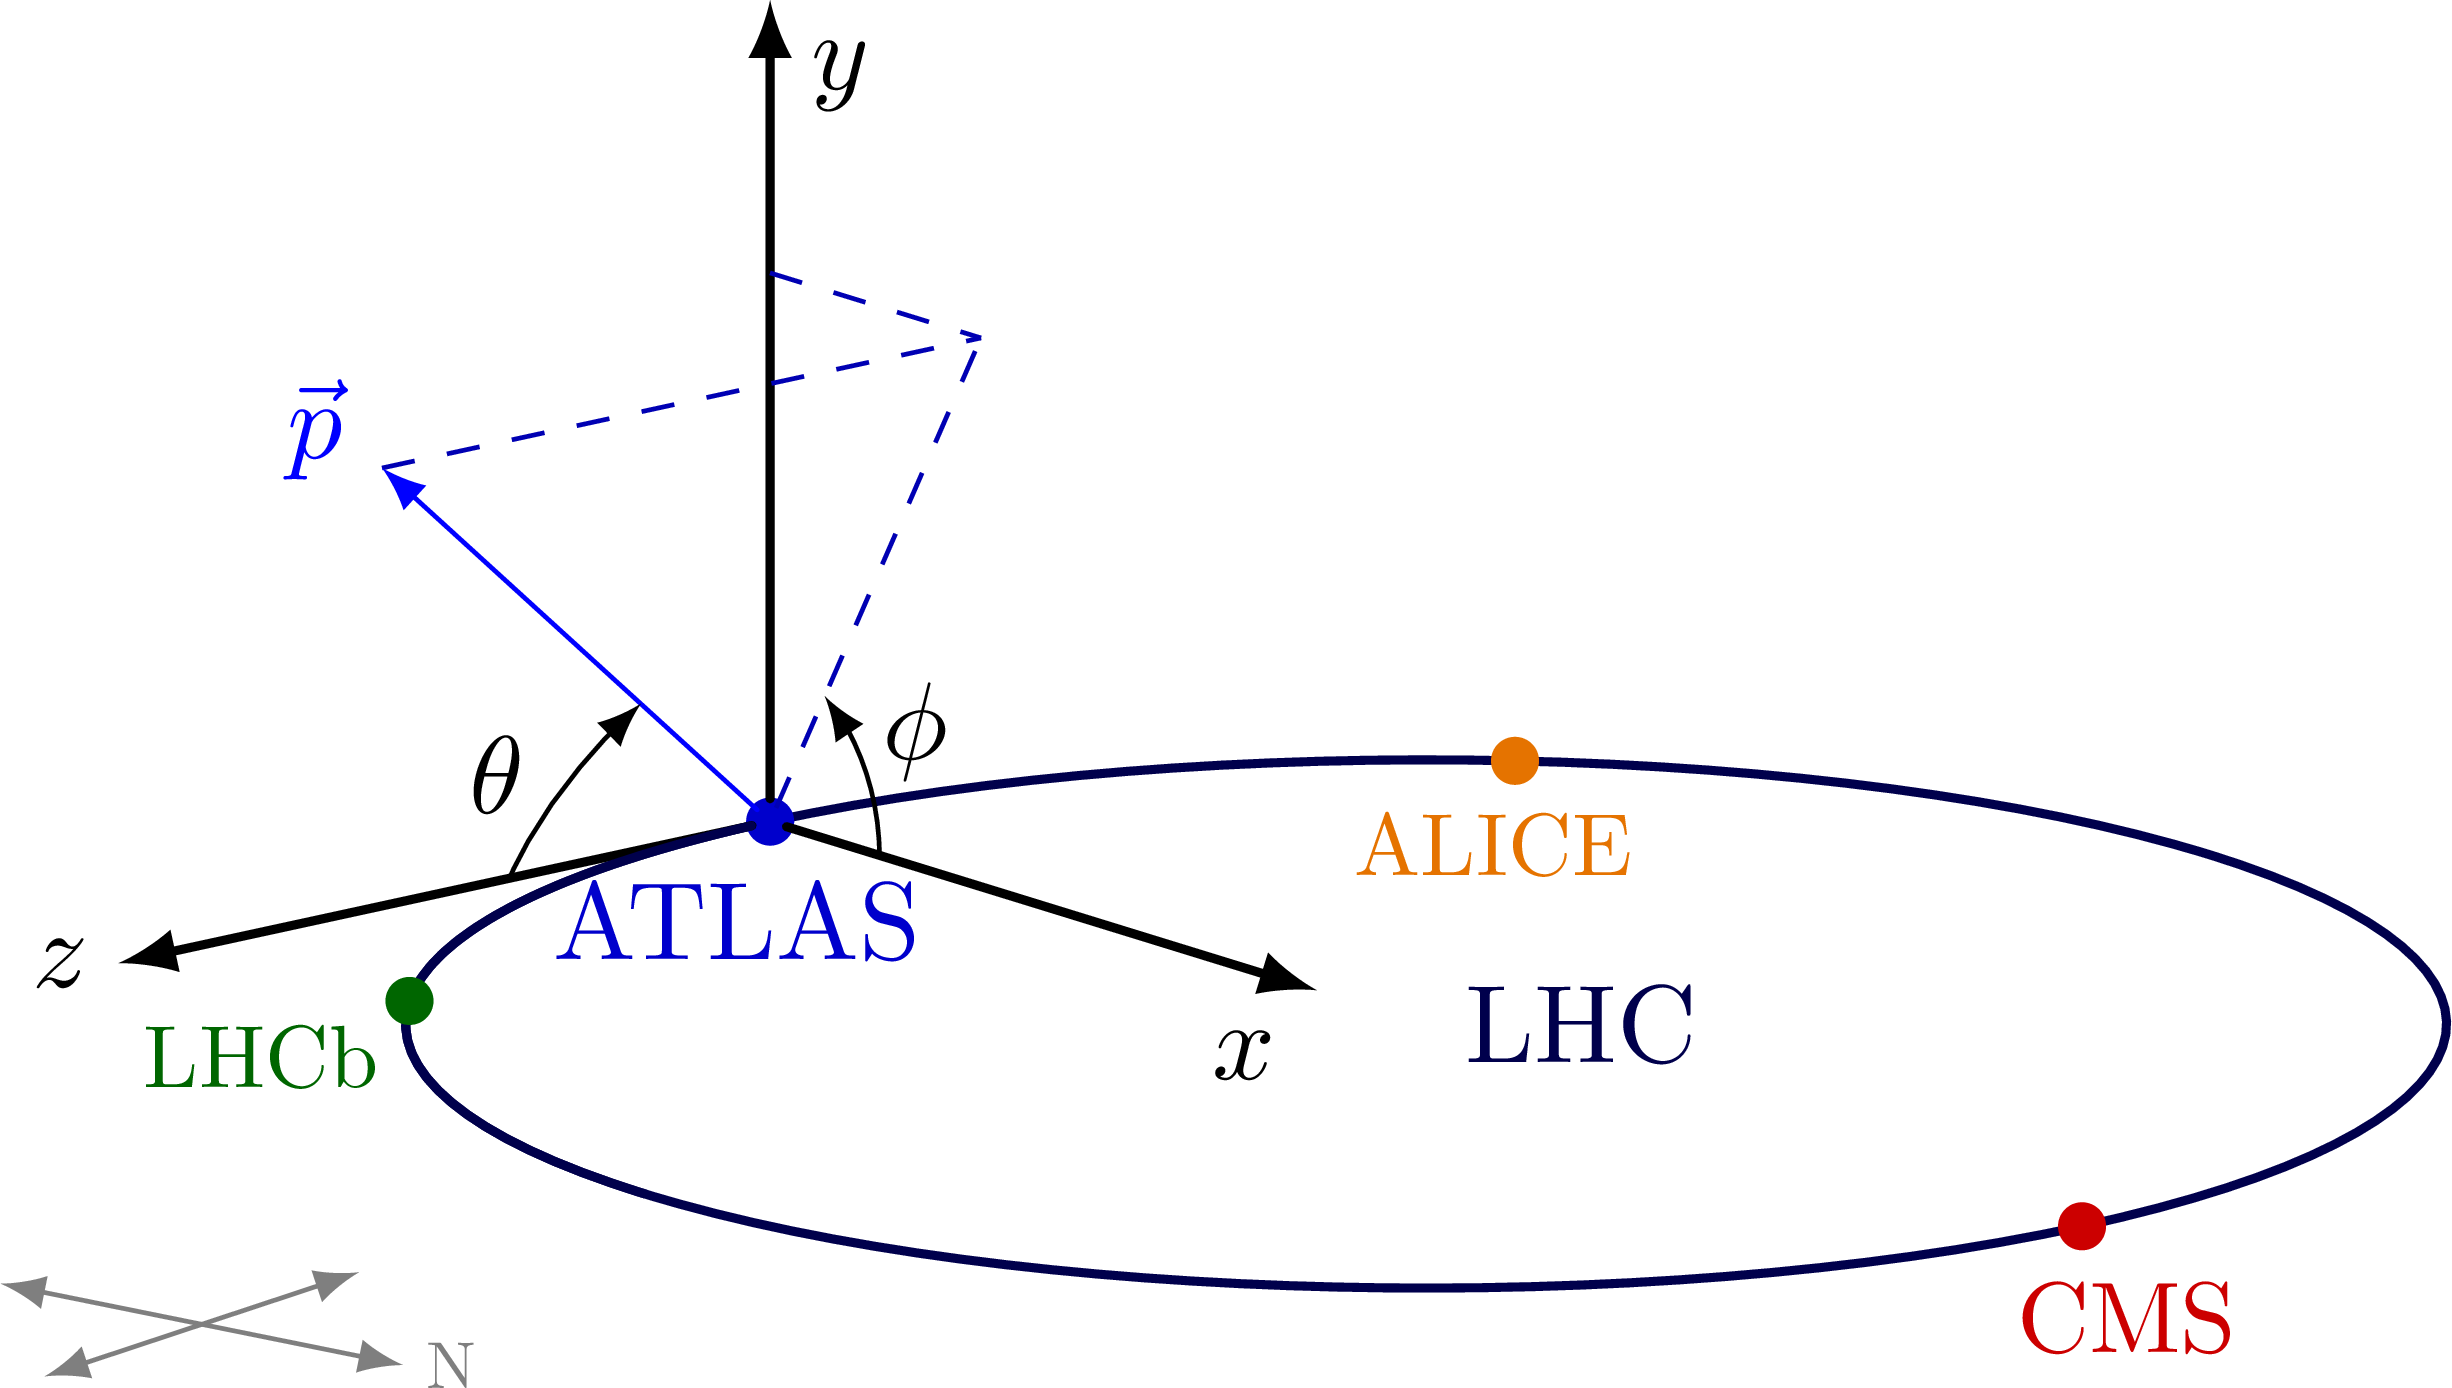
\includegraphics[width=0.7\textwidth]{plots/atlas/ATLAS_coordinates.png}
    \caption{The ATLAS coordinate system. Figure from \cite{Atlas:coordinates}.\label{fig:atlas_coordinates}}
\end{figure}

\subsection{Inner Detector}
The Inner Detector (ID) is comprised of three independent sub-detectors contained within a cylindrical envelope in a 2T solenoidal magnetic field. As charged particles travel through the ID, they ionise the material and leave behind a trail of electrical signals which are reconstructed to form tracks through the inner part of the ATLAS detector. The momentum can be inferred with high resolution from the curvature of the tracks. The ID also provides primary vertex (PV) and secondary vertex measurements (vertices are defined and discussed in Section \ref{sec:tracking}), and provides electron identification complimentary to the calorimeter. The ID covers the pseudorapidity range of $|\eta|<2.5$. In order of radial distance from the IP, the subdetectors consist of silicon pixel layers (Pixel detector), silicon microstrip layers (SCT detector), and layers of gaseous straw-tube elements called the Transition Radiation Tracker (TRT detector).  
%TODO: Mention insertable B-layer. See "Electron and photon energy calibration with the ATLAS detector using data collected in 2015" paper,
\subsubsection{The Pixel Detector}
At the inner radii, the highest resolution silicon sensors are required due to the difficulties in resolving tracks close to the IP. As such, the Pixel detector consists of three cylindrical silicon layers with individual sensor elements of $50\times400\mu\mathrm{m}^2$. The Pixel sensor elements are made up of 16 Front-End (FE) readout ASICS connected to a thin (250\microns) layer of silicon. When a charged particle travels through one of the pixel sensor elements, silicon atoms are ionised and liberated electrons travel through the bump bonds to the FE electronics. There are 2880 readout cells per FE ASICS chip. The readout cells of the FE amplify the sensor charge signal and compare it to a programmed discriminator threshold. For each readout, the hit pixel address, time stamp and amplitude information is transferred to buffers at the bottom of the FE.% Once the hit information is in the buffer, events are accepted depending the ATLAS Level-1 (L1) trigger decision, which happens every 2.5\microseconds. The transfer of the buffer content associated with one or more bunch-crossings is made to a readout driver (ROD) off the detector.

The top of the sensor elements contain a layer of kapton film onto which a Printed Circuit Board (PCB) is mounted containing a number of Surface Mounted Devices (SMDs) such as a temperature sensor, decoupling capacitors, and the Module Controller Chip (MCC). The MCC is responsible for Timing, Trigger and Control (TTC) logic tasks such as rejecting events where there are too many ($>15$) hits triggered in the FEs. The MCC is also responsible for extracting ordered hits from the FE and preparing them for transmission out of the pixel module \cite{Atlas:MCCmodule}.% A schematic view of a barrel pixel module is shown in Figure \ref{fig:atlas_pixelbarrelmodule} \cite{Atlas:MCCmodule}.
%\begin{figure}
%    \centering
%    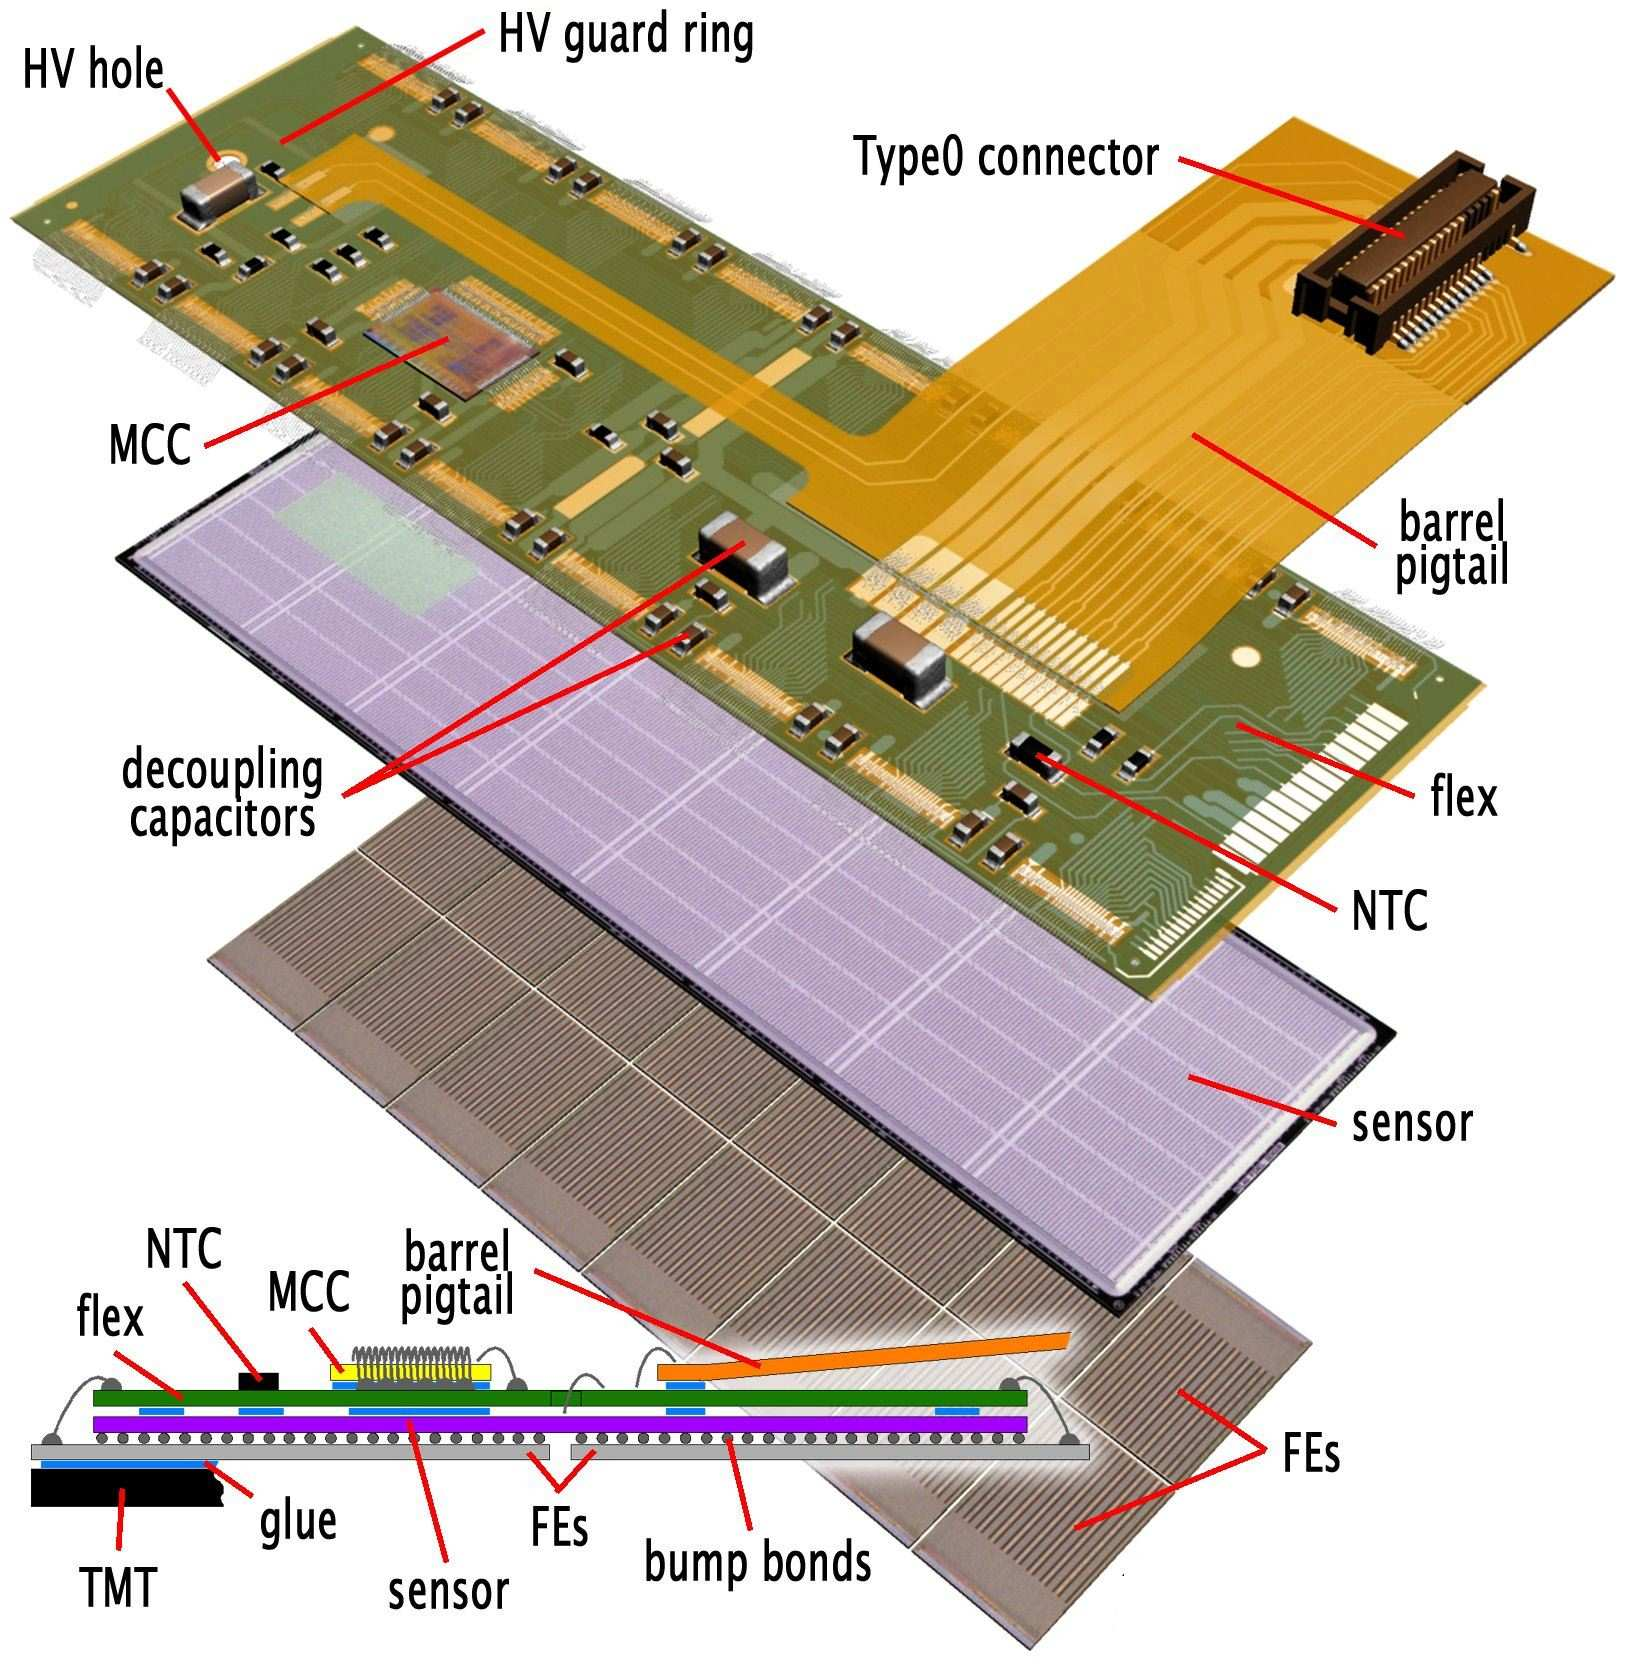
\includegraphics[width=0.5\textwidth]{plots/atlas/pixeldetectormodule.png}
%    \caption{A schematic diagram of one of the barrel pixel modules for the ATLAS ID system. In order of increasing radial distance from the beam, the FE ASICS, Si sensor tiles, and PCB with SMDs including the MCC are shown. A cross-section view of one of the barrel pixel modules is also shown.\label{fig:atlas_pixelbarrelmodule}}
%\end{figure}
%Remember to say something about radiation hardness (maybe operating temperature range?), and maybe something about the endcap modules maybe mention the spatial resolution ". At normal incidence, a spatial resolution of 12 µm is measured and approximately 80\% of the tracks have a single pixel hit. The resolution is not significantly degraded after irradiation. The optimal resolution of 4.7 µm (before) and 6.0 µm (after) irradiation is obtained for incident angles of 10–15deg (page 63 atlas design report) .
\subsubsection{The Semi-Conductor Tracker (SCT)}
The SCT enhances the high-resolution pattern recognition abilities of the ID at high radii, and consists of 4088 modules, arranged in four cylindrical layers in the barrel region and two end-caps, each containing nine disk layers. Each module consists of four sensors, with two sensors each on the top and the bottom side. A hybrid\footnote{Here, hybrid technology refers to the use of carbon-fibre substrates that have been directly interfaced with thin-film (polyamide) circuits to produce low-mass, thermally conductive, and radiation hard devices \cite{Atlas:Hybrids}} assembly bridges the sensors on each side. The top and bottom sensors are rotated through a relative ``stereo'' angle. In order to achieve the design azimuthal (the R-$\phi$ plane) and radial (R) resolutions of 17\microns and 580\microns respectively, the sensors are rotated at an angle of 40mrad. The silicon sensors are connected to binary signal readout chips.
%\begin{figure}
%    \centering
%    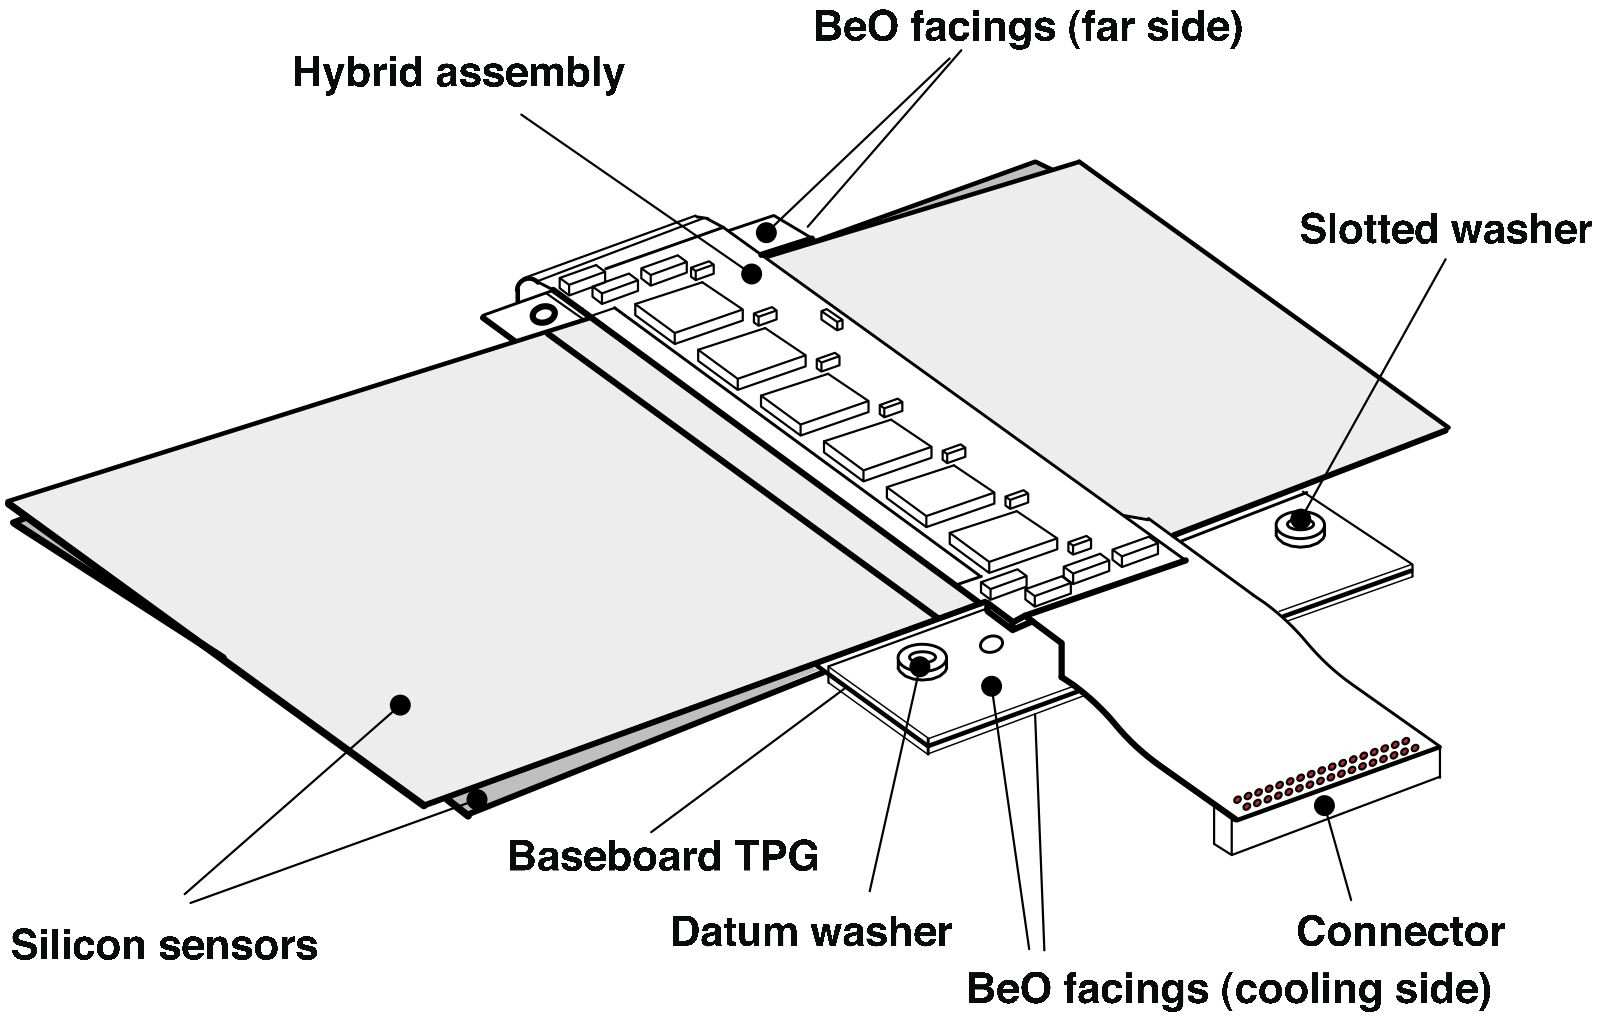
\includegraphics[width=0.75\textwidth]{plots/atlas/SCTmodule.png}
%    \caption{Drawing of a barrel SCT module. The Thermal Pyrolytic Graphite (TPG) material that comprises the baseboard conducts heat from the sensors to the octafluoropropane ($\mathrm{C}_3\mathrm{F}_8$) evaporative cooling system. The ceramic material Beryllia (BeO) is used on the surface layer of the TPG baseboard and is chosen due its high thermal conductivity and low density.\cite{Atlas:ThermalTechnologies} \label{fig:atlas_sctmodule}}
%\end{figure}
%The readout system for the SCT shares a number of common elements with the pixel and TRT. Namely, the same method of time-stamping, the use of buffers compatible with the L1 trigger latency, and the transfer to a ROD following an L1 trigger decision - note the ID is not part of the L1 trigger. The L1 trigger decision is made based on the calorimeters and muon detectors via the Central Trigger Processor (CTP). 
The readout hybrid on each SCT module contain 12 ASICs, with a total of 1536 readout channels. For each channel, there is a pre-amplifier, signal discriminator, and a shaper (splits each signal into overlapping channels, and applies a filter to optimise the signal/noise ratio). A buffer stores the hit information for approximately 3.2\microseconds, to allow for the L1 trigger decision (discussed in Section \ref{sec:ATLAS:trig}). 
\subsubsection{The Transition Radiation Tracker (TRT)}
The TRT enhances the performance of the ID at large radii, and consists of a barrel section and two end-cap sections. The basic elements of a TRT detector module are 4mm diameter polyimide straw tubes reinforced using carbon fibre bundles which stabilise the straw geometry by providing protection against environmental factors such as humidity and temperature. The straw tube walls are comprised of two multi-layer 35\microns thick films bonded back-to-back. Each tube contains a 31\microns diameter positively charged tungsten wire plated with 0.5-0.7\microns gold, directly connected to the front-end electronics. The tubes are filled with a mixture of 70\% Xe, 27\% C$\mathrm{O}_2$, and 3\% $\mathrm{O}_2$ gas. The gold plated wires act as anodes, attracting electrons liberated by charged particles and photons interacting with the gas mixture. The films contain a layer of aluminium, ensuring the sufficient electrical conductivity of the tube which acts as a cathode attracting positively charged ions \cite{Atlas:trt_designreport}.%next, put in citations, figure caption with all the explanation for the different elemtns of the film
%\begin{figure}
%    \centering
%    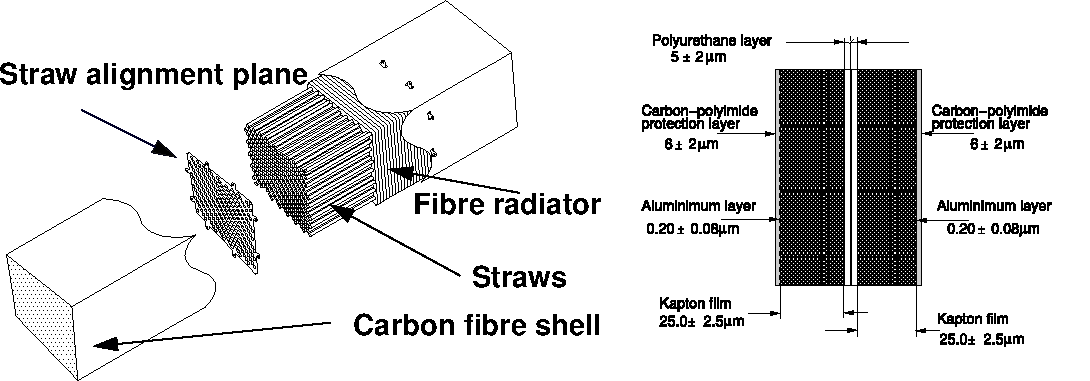
\includegraphics[width=\textwidth]{plots/atlas/trt.pdf}
%    \caption{Left, cut-out of one of the TRT barrel modules comprised of a carbon-fibre shell and polyimide straw tubes. Right, design of the (back-to-back) multi-layer film from which the straw tubes are manufactured. An aluminium layer on top of the kapton (polyimide) film enhances the electrical conductivity. The top carbon-polyimide layer protects the aluminium from damage from cathode etching effects. The polyurethane layer acts as a heat-activated adhesive and sealant. Figure adapted from \cite{Atlas:trt_module} and \cite{Atlas:trt_designreport}\label{fig:trt}.}
%\end{figure}
\subsection{Calorimeters}
%Two calorimeters - Tile and LAr. Full phi symmetry and coverage. Closest to beamline three cryostats - one barrel, two endcaps. Barrel: EM barrel calo, end cap cryostats: EM endcap calo; Hadronic EC calo; forward calo. Active detector medium is LAr, linear behaviour, stability of response over time, radiation hardness.
%
The ATLAS calorimetry system consists of electromagnetic (EM) and hadronic calorimeters. These are \textit{sampling} calorimeters, meaning that they are comprised of separate materials for inducing particle showers and for detecting the energy of the particles. Due to superior energy resolution, the energy measurements of most charged and neutral particles are provided by the calorimeters (rather than the tracking system). The electromagnetic calorimeters primarily make measurements of electrons and photons. The energy measurements of hadrons are primarily derived from signals in the hadronic calorimeter system.%The active media of the hadronic calorimeter system are scintellator sheets for the tile calorimeter and liquid Argon for the hadronic end-cap and forward calorimeters. Hadron energy losses occur primarily through nuclear interactions resulting in hadronic showers. 
%\newline
%Closest to the beamline, the calorimeters consist of sampling detectors with full $\phi$ coverage. These calorimeters are the electromagnetic barrel calorimeter, Electromagnetic End-cap Calorimeter (EMEC), Hadronic End-cap Calorimeter (HEC), and the Forward Calorimeter (FCAL). The detector medium for all these calorimeters is liquid Argon.
%\newline
\subsubsection{The EM Calorimeters}
The EM barrel and end-cap calorimeters have an accordion geometry and are comprised of lead and stainless-steel absorbers, LAr active material, and copper readout electrodes, which are positioned in the gaps between the absorbers. There are three active layers in the central region ($0 < |\eta| < 2.5$), and two in the forward regions $(2.5 < |\eta| < 3.2)$. The first layer is read out front, which is defined as the inner radius of the EM barrel, and the small-$z$ region of the end-cap. Conversely, the second and third layers are read out from the back. The barrel EM calorimeter is made up of two halves covering $|\eta|<1.475$. The cell granularity in $\Delta\eta\times\Delta\phi$ is $0.025/8\times0.1, 0.025\times0.025$, and $0.050\times0.025$ in the first, second, and third layers respectively, for $|\eta|<1.40$. In the $|\eta|>1.40$ region, the cell granularity is significantly coarser. The end-cap regions cover the $1.375<|\eta|<3.2$ range. The cell granularity in this region is the finest in the central part of the coverage range. The first layer has a granularity of $0.025/8\times0.1$ at $1.5<|\eta|<1.8$, and the granularity becomes coarser towards the limits of the end-cap coverage.  There is a crack region at $1.37<|\eta|<1.52$ where the transition between the barrel and end-cap calorimeters takes place. There is also a small crack at $|\eta|=0$ due to the fact that the calorimeter half-barrels are separated by 6mm at $z=0$.

When electrons and photons interact with the stainless-steel absorbers, narrow particle showers are produced as a result of a combination of bremsstrahlung, $e^{\pm}\rightarrow e^{\pm}\gamma$, and $\gamma\rightarrow e^+e^-$. Repeated interactions of the produced particles results in a cascade of particles with decreasing energy, which continues up until the pair production energy threshold. Below this threshold, photon energy losses occur primarily via compton scattering and the photo-electric effect, and the shower ceases. The characteristic amount of matter traversed by a particle before undergoing bremsstrahlung or pair production is the radiation length $X_0$, which is used to quantify the amount of material used in the calorimeter layers. The expectation values of the energies of the electrons $E(x)$ and intensity of the photons $I(x)$ in the shower follow exponential decay laws, with the decay constant determined by the radiation length
\begin{equation}
    \langle E(x)\rangle = E_0\mathrm{e}^{-\frac{x}{X0}},\hspace{20pt} \langle I(x)\rangle = I_0\mathrm{e}^{-\frac{7}{9}\frac{x}{X0}},
\end{equation}
where $x$ is the distance of the traversed material.
The EM calorimeters are complemented by pre-samplers which provide measurements of energy losses incurred by particles in the inner detector, i.e. before they interact with the calorimeter material.

\subsubsection{The Hadronic Calorimeters}

Hadrons interact with the nuclei of the absorbers via the strong force, resulting in the production of hadrons, especially pions. Each hadron undergoes additional interactions to form a cascade. Through nuclear de-excitation, lower energy neutrons, protons, $\alpha$-particles and photons are also produced. The hadronic shower also has a substantial electromagnetic component, which comes about primarily due to the decays of neutral pions \cite{Atlas:particleintmatter}. Hadronic showers are characterised by the nuclear interaction length $\lambda$, which is a function of the inelastic cross-section of the scattering process. Nuclear interaction lengths are typically an order of magnitude larger than radiation lengths, which explains why the ATLAS hadronic calorimeter system is larger than the EM calorimeter system \cite{Buckley:PCP}.

Hadronic showers represent a number of challenges. There are a considerable number of sources of energy leakage, such as backscattering and nuclear excitation processes, which do not result in an observable signal. In this way, the ATLAS calorimeter system is \textit{non-compensating}. This means that the calorimeter response (the ratio of the average calorimeter signal to the energy of the particle) is smaller for non-EM components of hadron showers than for EM components. Additionally, there are large fluctuations in the fraction of the EM and non-EM components of the larger hadronic shower. All of this degrades the hadronic energy resolution. 

The three hadronic calorimeters correspond to the Tile, the Hadronic End-Cap (HEC), and the Forward Calorimeters (FCal). The Tile calorimeter is comprised of an array of steel absorbers and scintillator sheets as the active medium. The Tile calorimeter comprises three layers, and covers the region $|\eta|<1.7$, behind the EM calorimeter, and has a radial depth of about $7.4\lambda$. The $\Delta\eta\times\Delta\phi$ cell granularity in the first two layers is $0.1\times0.1$, and $0.2\times0.1$ in the last layer. The scintillator signals are read out by photomultiplier tubes coupled to each tile edge through a series of fibres. The Tile calorimeter has a total of 187456 readout channels \cite{Atlas:design}.

The HEC calorimeter uses copper as the absorber and liquid-argon as the active material. The HEC comprises four layers, which cover the range $1.5 < |\eta| < 3.2$. The HEC calorimeter has a radial depth of about $9.7\lambda$. The $\Delta\eta\times\Delta\phi$ cell granularity is $0.1\times0.1$ at $1.5<|\eta|<2.5$, and $0.2\times0.2$ at $2.5<|\eta|<3.2$. The gaps between the plates that comprise the HEC modules contain the readout modules, which are made up of three electrodes separated by honeycomb spacers. The central electrodes contain readout cells of size $\Delta\eta\times\Delta\phi=0.1\times0.1$ in the $|\eta|<2.5$ region and $0.2\times0.2$ for larger values of $|\eta|$. The HEC calorimeter contains 5632 readout channels \cite{ATLAS:HEC,Atlas:design}.

The FCal extends the calorimeter coverage into the forward regions ($3.1 < |\eta| < 4.9$), and has a radial depth of about $10\lambda$. The FCal comprises one electromagnetic module (FCal1) and two hadronic modules (FCal2, FCal3). The $\Delta\eta\times\Delta\phi$ cell granularities are $3.0\times2.6, 3.3\times4.2$, and $5.4\times4.7$ in the central cells of the FCal1, FCal2, and FCal3, respectively, and the granularities are around four times finer around the coverage limits. Copper is used as the absorber for FCal1 to optimise the energy resolution of measurements of EM showers, and tungsten is used as the absorber in FCal2 and FCal3 to contain the lateral spread of hadronic showers. Each of the FCal modules contain readout electrodes which are connected to the module faces. Signals are read out from the side nearer to the interaction point for FCal1, and from the side furthest from the interaction point for FCal2 and FCal3. The FCal calorimeter contains 1762 readout channels \cite{Atlas:design}.

\subsubsection{Energy Resolution}
The energy resolution defines the most important attributes of the ATLAS calorimeter system and is often quoted as follows
%
\begin{equation}
    \label{eq:energyres}
    \frac{\sigma(E)}{E}=\frac{a}{\sqrt{E}}\oplus\frac{b}{E}\oplus c\%,
\end{equation}
%
where $\oplus$ denotes addition in quadrature. The $a$ term is the \textit{stochastic} term, which primarily arises due to fluctuations in the number of particles produced in the shower. This term limits the low-energy performance of the calorimeters. The $b$ term describes electronic noise primarily from readout electronics, and the $c$ term is a constant term which dominates in the high energy limit. Measurements of the calorimeter energy resolutions are made using lepton and hadron test-beams. Results from these measurements are shown in Figure \ref{fig:energyres}. Note that for the LAr energy resolutions results using electron test-beams are fitted with equation \ref{eq:energyres}, without the $\frac{b}{E}$ term. This is because a noise-subtraction step is implemented for every energy measurement since the noise here depends on the gain of the LAr calorimeter cells. The pion test-beam results for the combined calorimetry shown in Figure \ref{fig:energyres} utilises the full functional form of equation \ref{eq:energyres}. %Note that since the noise depends on the gain of the calorimeter cells (which is non-uniform with energy), for the LAr energy resolution measurements using lepton test beams, a noise-subtraction step in implemented for each energy point to obtain the intrinsic resolution of the calorimeter. Hence, for these measurements the energy resolution measurements after noise-subtraction are fitted using equation \ref{eq:energyres}, without the $\frac{b}{E}$ term.

\begin{figure}[t]
    \begin{minipage}{6in}
        \centering
        \raisebox{-0.5\height}{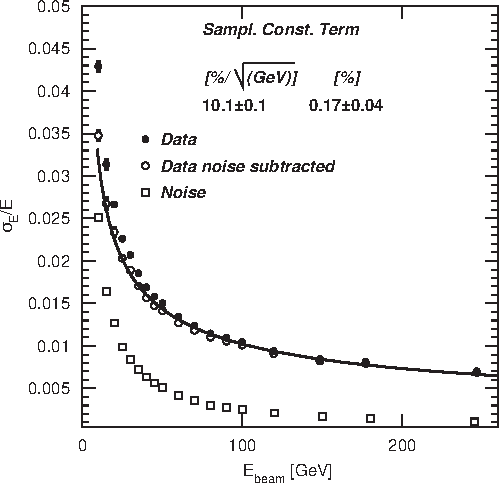
\includegraphics[width=0.40\textwidth]{plots/atlas/energy_resolution.pdf}}
        \hspace*{.2in}
        \raisebox{-0.5\height}{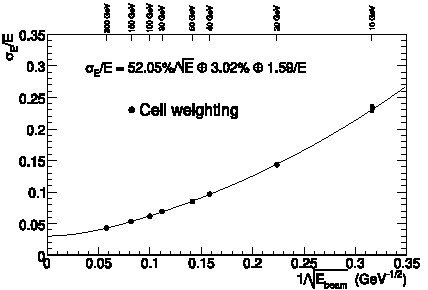
\includegraphics[width=0.53\textwidth]{plots/atlas/pion_energy_resolution_LAR_TILE.pdf}}
        \centering
    \end{minipage}
    \caption{Fractional energy resolution in the ATLAS EM barrel calorimeter as a function of the beam energy obtained from electron test-beams at $|\eta| = 0.687$ (left). Fractional energy resolution obtained using pion test beams for combined LAr and tile calorimetry at $|\eta|=0.25$ (right). The energy resolution for pion test-beams is shown as a function of $1/\sqrt{E_{\text{beam}}}$. Markers corresponding to $E_{\text{beam}}$ are shown at the top of this plot for the ease of comparison. 100$\GeV$ electrons have an energy resolution of about $1.1\%$ in the central region of the calorimeter system, compared to about $6.2\%$ for hadrons. Note that in regions where the forward calorimetry (FCal) system is in use ($3.1 < |\eta| < 4.9$), the energy resolution increases to about 5$\%$ for 100\GeV electrons, and to about $8\%$ for $100\GeV$ pion test-beams \cite{Atlas:EMCalo,Atlas:design}.\label{fig:energyres}}
\end{figure}

\subsection{Muon Spectrometer}

The muon spectrometer (MS) covers the pseudorapidity range of $|\eta|<2.7$. The MS measures charged particles (primarily muons) that penetrate the barrel and end-cap calorimeters. The primary purpose of the MS is to identify and measure high momentum muons. The MS is designed to measure the transverse momentum of muons with $\pt>1\TeV$ to an accuracy of $10\%$. The MS is also capable of triggering on muon tracks, and is designed to trigger in the region of $|\eta|<2.4$. The precision momentum measurements of the MS system are provided by Monitored Drift Tube (MDT) chambers and Cathode-Strip Chambers (CSC). This is complemented by Resistive Place Chambers (RPC) and Thin Gap Chambers (TGC) which provide fast triggering capabilities to clarify events of interest. 

The MS is partitioned in the barrel and endcap regions into three layers referred to as the inner, middle, and outer layers. Two MDT chambers are housed in each of the layers. There are a total of twelve MDT segments in radially consecutive stations (collection of segments in a layer) spanning three layers. The CSCs are located in the inner endcap layer. Both the CSCs and MDTs are segmented into large and small chambers. The RPC system is layered into three trigger stations and is comprised of large and small small segments. The RPCs are located in the middle and outer layers of the barrel. The TGC system is comprised of seven layers in the EM layer, and two layers in the inner endcap layer.
%\begin{figure}
%    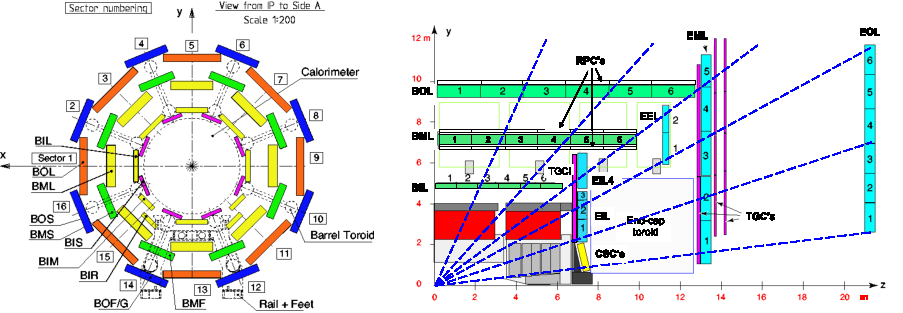
\includegraphics[width=\textwidth]{plots/atlas/ms.pdf}
%    \caption{Cross-sections of the barrel muon system perpendicular to the beam axis (left), and in the bending plane containing the beam axis (right). In the right figure, the blue dashed lines represent muon trajectories in the absence of a magnetic field. Figure from \cite{Atlas:design}. \label{fig:ms}}
%\end{figure}
%\newline

The MDTs cover the pseudorapidity range of $|\eta|<2.7$ in all but the inner most layer. The MDTs are drift tubes with a diameter of about 3cm, and are pressurised with a mixture of Ar and $\text{CO}_2$ gas. The centers of the tubes contain a $50\mu m$ diameter tungsten-rhenium wire. When a charged particle enters the tube, the gas is ionised, and liberated electrons drift to the wire and the ions drift to the walls of the tube. 

The MDTs provide a position resolution of $80\microns$. The position measurements are determined by the drift time of the charges deposited in the MDTs. Muon tracks are reconstructed using these measurements, and this is discussed in more detail in Section \ref{sec:muon}. The $\pt$ of the muon is directly inferred from the radius of curvature of the tracks. For the required momentum resolution, a sagitta \footnote{The perpendicular distance between the apex of the arc of the track, and the chord intersecting the inner and outer layers of the MDT.} along $z$ of about $500\mu m$ needs to be known with a resolution better than $50\mu m$.  

The CSC system covers the forward $2<|\eta|<2.7$ region. The CSC system are two disks of eight wire chambers. Each chamber is filled with an Ar$\text{CO}_2$ gas mixture and contains an array of high voltage anode wires and cathode planes at ground potential. Precision position measurements in both $R$ and $z$ are obtained with a resolution of $60\mu m$ via measurements of the charge distributions on the cathodes.

The muon trigger system consists of RPCs and TGCs. The RPCs are used in the barrel region ($|\eta|\leq 1.05$), and TGCs in the  end-cap region ($1.05\leq|\eta|\leq 2.4$). Different technologies are used in different regions due to different requirements on spatial and timing resolution as well as considerations of trigger rate. The RPCs are gaseous parallel electrode-plate detectors. These are comprised of two parallel dielectric plates separated by 2mm. In the 2mm gap is a gas mixture, and a high electric field is applied (4kV/mm) between the plates. When a charged particle travels through the gas gap, the gas is ionised, and the positive ions travel towards the cathode, and the electrons towards the anode. The liberated electrons are accelerated by the high electric field to a sufficient extent such that they go on to liberate additional electrons from the gas medium resulting in a chain reaction of ionisation events. This process is known as a Townsend avalanche \cite{ATLAS:townsend}. The electrical signals from the avalanches are read out via metallic strips mounted on the outer faces of the resistive dielectric plates. TGCs operate on the same principle as the wire chambers of the CPC. The primary function of the RPCs and TGCs are to facilitate triggering on muon events, but they also complement the MDT tracking data. Through the additional measurement of the track coordinates in the non-bending $\phi$ plane, which complement the measurement in the bending $\eta$ plane, the MDT and RPC (and TGC in the end-cap region) measurements can be combined in an unambiguous way \cite{Atlas:design,ATLAS:MS}.

\subsection{ATLAS Trigger and Data-acquisition\label{sec:ATLAS:trig}}
The ATLAS trigger and data-acquisition (TDAQ) system is responsible for deciding which events from of the $\num{40e6}$ bunch-crossings per second at the ATLAS interaction point to save for physics analyses, calibrations, monitoring, and performance measurements. The trigger system is comprised of two stages. These are the Level-1 (L1) and HLT triggers. 

The hardware based Level-1 trigger is principally responsible for making the trigger decision to reduce the event rate from 400MHz to maximally 100kHz by processing signals from the calorimeters and MS. The L1 trigger consists of the L1Calo, L1Muon, L1Topo, and Central Trigger subsystems. The L1Calo comprises the Cluster Processor (CP) and Jet/Energy-sum Processor (JEP), which receive calibrated calorimeter signals in parallel to identify physics object candidates. Tile calorimeter and MS information is passed to the L1Muon, where searches are performed for signals consistent with muons originating from the interaction point. The L1Topo receives object candidates from the L1Calo and L1Muon in order to reconstruct topological observables such as invariant masses and angular observables. The outputs from the L1Calo, L1Muon and L1Topo are processed by the Central Trigger Processer (CTP) which makes the L1 trigger decision. The CTP is also responsible for applying a preventative \textit{dead-time} mechanism to moderate the L1 accept rate. For every L1 trigger decision, ``Regions Of Interest'' (RoIs) are identified using $\eta$ and $\phi$ information \cite{Buckley:PCP,Atlas:tdaq,Atlas:willL1Trigger}. 

After a L1 trigger accept, the events are processed by the software-based High-Level Trigger (HLT). Events processed by the HLT use fine-granularity calorimeter and precision MS information, as well as tracking information from the ID. The HLT performs the event reconstruction within the L1 RoIs or the full detector, as needed. In most cases, the HLT performs a fast first-pass reconstruction using a sequence of \textit{feature-extraction} algorithms. A trigger decision is then subsequently made by the \textit{hypothesis} algorithms. Afterwards, more precise and computationally expensive algorithms reconstruct high level physics objects in greater detail -- this is called the \textit{online reconstruction}. The online reconstruction of objects is less precise, but nevertheless similar to the offline reconstruction (Section \ref{sec:objreco}). Events passing the HLT decision are saved to the CERN Tier-0 computer centre for offline reconstruction, this occurred at a rate of approximately 1.2kHz during the 2018 data taking for Run-2 for triggers dedicated to physics analyses \cite{Atlas:tdaq,Atlas:trig2015}. 

Each combination of L1 and HLT event selections has an associated set of \textit{prescale} factors, which take values of at least 1. A prescale value of $n$ means that an event has probability of $1/n$ of being kept. Prescales are defined for both L1 and HLT, but the prescale is implemented slightly differently in each case. For L1 prescales, since the CTP is fast, the trigger decision is still computed for every event, but for each event that passes the trigger decision, a random number generator determines whether it is passed to the HLT. Since the online reconstruction is expensive, HLT prescales are applied before the trigger decision is computed. The reason for applying prescales is to prevent saturating the allowed bandwidth. This is possible for certain processes, such as minimum bias, which have very loose triggers and therefore very high event rates \cite{Buckley:PCP}.

A combination of L1 and HLT prescales and event selections comprises an item in the \textit{trigger menu}, which consists of a list of:
\begin{itemize}
    \item \textit{Primary} triggers: used for physics analyses, usually unprescaled.
    \item \textit{Support} triggers: used for monitering, performance, and efficiency measurements. These are usually prescaled, and have small HLT rates of around 0.5Hz
    \item \textit{Alternative} triggers: used in the commissioning of new triggers. These use alternative reconstruction algorithms, and are complimentary to primary triggers
    \item \textit{Backup} triggers: used in case CPU usage or output rate of primary triggers too high. These are similar to primary triggers but with tighter selections.
    \item \textit{Calibration} triggers: used for detector calibrations, and run at high rates. 
\end{itemize} 
All items in the trigger menu are connected to an HLT data stream. The \textit{Main} physics stream contains events for physics analyses, and a small fraction of these events are written to the \textit{Express} stream which is used to derive offline calibrations soon after data taking. There are about twenty additional streams for calibration, monitoring and detector performance studies in addition to specialised \textit{Trigger-Level Analysis} and \textit{debug} streams. The physics \textit{Main} stream events are partitioned into categories called trigger signatures, for example ``single leptons''. Each trigger signature is split up into multiple items giving the L1 and HLT trigger thresholds, object multiplicities, online object isolation requirements, as well as peak trigger rates. For example, for an offline selection of a single isolated muon with $\pt>27\GeV$, the corresponding trigger in the 2018 trigger menu corresponds to a 20\GeV single muon requirement at L1, a 26\GeV isolated muon at HLT, with a peak L1 trigger rate of 16kHz, and peak HLT trigger rate of 218kHz. The values of the offline \pt values in the trigger menu are usually defined as the value where the trigger efficiency\footnote{The trigger efficiency is the number of correctly identified objects divided by the actual number of objects above a certain \pt threshold. At the LHC, typically trigger efficiencies of $>90\%$ (10\% accuracy) are deemed acceptable \cite{Atlas:triggeratlhc}.} plateaus \cite{Atlas:trigmenu}.
%single lepton triggers
%Include a few sentances on how the online resonstruction differs from the offline

\subsubsection{Photon and Lepton Triggers}
%Mention figure for e/y trigger reco.  

Electron and photon candidate RoIs are identified in the L1 trigger using only calorimeter information in the central ($|\eta|<2.5$) region. The identification works by iterating over groups of EM calorimeter cells, called ``trigger towers'', of size $2\times2$ ($\Delta\eta\times\Delta\phi = 0.1\times0.1$). Within each $2\times2$ region, the \et of all the four possible $1\times2$ and $2\times1$ pairs of towers is calculated. If the maximum \et among these pairs passes the L1 \et threshold (nominally 22\GeV), the $2\times2$ region is identified as an RoI. An additional hadronic activity veto can be applied, where candidates are rejected if the $2\times2$ hadronic calorimeter trigger towers behind the EM cluster have an \et above a given threshold. An isolation requirement can also be defined by a threshold on the energy of the EM isolation ring around the $2\times2$ RoI. Figure \ref{fig:triggertower} shows a schematic view of the EM and hadronic trigger towers \cite{Atlas:trigegamma,Atlas:trig2015}.
\begin{figure}[t]
   \centering
   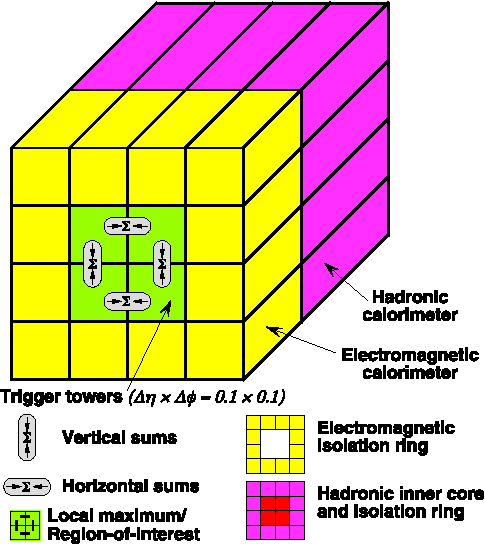
\includegraphics[width=0.6\textwidth]{plots/atlas/triggertower.pdf} 
   \caption{Layout of the trigger towers used in the L1 trigger electron and photon reconstruction. The EM calorimeter cells are colored in yellow, and the majenta cells denote the hadronic calorimeter cells. Figure from \cite{Atlas:trig2015}.\label{fig:triggertower}}
\end{figure}

 % The online-reconstruction differs in that the GSF refit is not performed for electron tracks, only topo-clusters are used (rather than variable-sized superclusters), and for the assessing of pileup, only information from the average number of interactions per bunch crossing, $\langle\mu\rangle$ is used, rather than the number of primary vertices. Additionally, some cell energy and pileup corrections are not implemented for the online-reconstruction. In the 2x2 central region of the towers, all possible 1x2 or 2x1 pairs of cell energies are summed, and if a predefined \et threshold is reached, the 2x2 region is flagged as a RoI.
The reconstruction of electrons and photons at the HLT is performed in each RoI identified by the L1 trigger. For the fast stage of the HLT decision, a cut-based algorithm is used for electrons below $15\GeV$ and for the reconstruction of all photons. Objects are identified based on the \et of the cluster and the shape of the EM shower. %The algorithm starts by reconstructing clusters in the L1 RoI. For speed, use only the second layer of the EM calorimeter is used (since electrons and photons deposit most energy in second layer) to find the ``pre-seed'' cell, which is the cell with the largest \et. Regions of the calorimeter around the preseed are searched for the seed, the local maximum. Electrons and photons are then reconstructed using $3\times7$ (barrel) and $5\times5$ (endcap) clusters. Corrections derived from offline reconstruction algorithms are applied to improve the cluster energy and position resolutions. The object identification is based on the \et of the cluster and three shower shape variables. Above the $15\GeV$ threshold, a neutral-network based algorithm is used for electron reconstruction for the fast HLT step. For electrons, there is also a fast track reconstruction step performed inside the RoI.
%%%START HERE%%%
After the initial fast HLT decision, information from outside the RoI may be used, and the precision online-reconstruction is performed in a similar manner to the offline electron and photon reconstruction outlined in Section \ref{sec:egamma}. %The precision online-reconstruction differs in that the GSF refit is not performed for electron tracks, only topo-clusters are used (rather than variable-sized superclusters), and for the assessing of pileup, only information from the average number of interactions per bunch crossing, $\langle\mu\rangle$ is used, rather than the number of primary vertices. Additionally, some cell energy and pileup corrections are not implemented for the online-reconstruction. 

At the precision stage, there are optional requirements on the calorimeter-only isolation used in the photon triggers denoted by \textit{icalvloose} or \textit{icaltight} in the trigger menu. These operating points differ in the size requirements of the isolation cone around the photon candidate used for noise subtraction, and in the fraction of topo-cluster energy required to originate from the photon candidate. For the noise subtraction, the \textit{icalvloose} working point uses a cone size of $\Delta R=0.2$, and \textit{icalvloose} uses $\Delta R=0.4$. The ratio of the total topo-cluster \et to the photon-candidate \et is required to be $<10\%$ for \textit{icalvloose} and $<3\%$ for \textit{icaltight}.

For identifying electrons at the precision stage, a likelihood discriminant is constructed in a similar way to the offline-reconstruction. The likelihood discriminant operating points are: \textit{lhvloose}, \textit{lhloose}, \textit{lhmedium}, and \textit{lhtight}. For some electron triggers, the transverse impact parameter $d_0$, and its significance $|d_0/\sigma(d_0)|$ are not used in constructing the online discriminant. Such triggers are labelled with the suffix ``nod0''. A tracking-only isolation requirement called \textit{ivarloose} is also available for electron triggers \cite{Atlas:trigegamma}. 

\subsection{Data Processing \label{sec:dataproc}}
What happens upstream of the offline physics object reconstruction steps is different depending on whether real collider data or simulated event generator data is being processed. With real data, particles interact with the ATLAS subdetectors, and the data are retrieved from the detector readout hardware, after the Level1 and HLT trigger decisions, through the DAQ system. These raw signals are then passed through the offline reconstruction algorithms. For the case of simulated data, a detector simulation is used on the information from the MC event generator event record. ATLAS makes use of the GEANT4 \cite{GEANT4} program to perform this step. The output from this step is a collection of simulated energy deposits in the detector, called ``hits''. The raw hit information cannot be used to reconstruct physics objects, as these algorithms rely on information from the detector subsystem readout electronics. The process of ``digitization'' turns the hits into simulated detector responses (digits), which correspond to the electrical signals from the readout system.

After the building of physics objects via the offline reconstruction step, the output is a highly detailed collection of event data containing the physics objects as well as information pertaining to the raw detector readout or digits in the case of simulated events. This is called Event Summary Data (ESD). ESD is not used directly in a physics analysis. Instead, a reduced format called Analysis Object Data (AOD) provides the necessary physics object information. Since different analyses and calibrations have varying needs for information on the reconstructed objects, the AODs require filtering into smaller subsets which are actually used at an analysis level. These subsets are called derived AODs, or DAODs (also ``derivations''). At ATLAS, each combined performance and analysis subgroup have their own set of DAODs which are targeted at specific calibrations or physics analyses. The following terms are often used in the context of derivation production:
\begin{itemize}
    \item \textbf{Skimming}: where physics object cuts and trigger requirements are used to remove events.
    \item \textbf{Slimming}: the removal of unrequired computed quantities.
    \item \textbf{Thinning}: the removal of containers of physics objects \cite{Buckley:PCP}.
\end{itemize}

%detector information from simulated or recorded $pp$ collisions, the output is a highly detailed collection of event data. %These data pertaining to the physics objects, 
%After all the detector information from a given simulated MC or recorded data $pp$ collision event has undergone the initial processing   %The low-level output from 

\subsection{ATLAS Object Reconstruction\label{sec:objreco}}
\subsubsection{Tracks and primary vertices\label{sec:tracking}}
Tracks are described by five parameters relative to a reference point, as shown in Figure \ref{fig:trackcoords}. The transverse and longitudinal impact parameters ($d_0$ and $z_0$) are defined using the perigee (point of closest approach) of the track relative to the reference point. $d_0$ and $z_0$ are then the transverse and longitudinal distances of the perigee to the reference point, respectively. The other three parameters are the angles $\phi$ and $\theta$, which are the azimuthal and polar angles of the track momentum relative to the reference point, and the ratio $\frac{q}{|\mathbf{p}|}$, which is the ratio of the electric charge divided and the magnitude of the track momentum. The reference point for track reconstruction is defined as the ``beamspot'' position, i.e. the average position of the \textit{pp} interactions. See Figure \ref{fig:trackcoords} for a schematic view.
\begin{figure}[t]
    \centering
    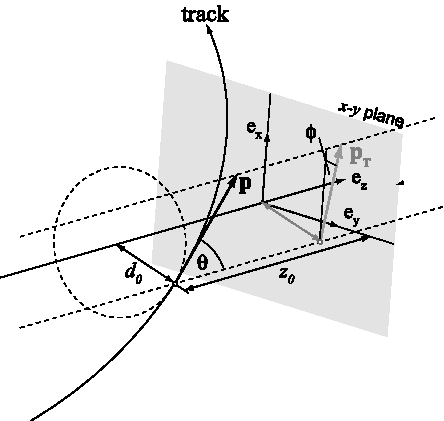
\includegraphics[width=0.6\textwidth]{plots/atlas/trackcoordinates.pdf}
    \caption{Schematic of the track coordinates defined using the perigee of the track. Figure from \cite{Atlas:trackcoords}\label{fig:trackcoords}.}
\end{figure}

Track reconstruction is partitioned into a primary tracking chain of algorithms followed by a back-tracking chain. %In the primary tracking, the track reconstruction is initiated by ``track seed'' formation in the pixel or SCT and in final step of, information from the TRT is used. The back-tracking chain is designed to resolve track ambiguities and is relevant primarily for the reconstruction of electron tracks from photon conversion. 
The primary tracking chain starts with track seed formation. Track seeds consist of a triplet of space-points (SP) in the pixel or SCT layers, which are consistent with originating from a charged particle track. Next, for each seed, a set of detector modules in the path of the track are identified. The seeds are extended using SCT and pixel clusters contained within those modules using a Combinatorial Kalman Filter \cite{Atlas:kalman}. This results in a set of potentially overlapping track candidates. Fake tracks also are reconstructed, which are incorrect combinations of unrelated pixel and SCT clusters \cite{Atlas:trackingsoftwaretut}.

A dedicated ambiguity resolution step is performed to reduce contributions from fake tracks. In this step, a score is given to each track candidate based on a number of criteria, and lower quality candidates are rejected if there are a large number of shared hits with higher quality tracks. After the ambiguity resolution, a global $\chi^2$ fit is performed to obtain the final track parameters. Finally, if an extension of the track into the TRT is possible, tracks are extended, and a re-fit of the entire track is performed. For electron and converted photon tracks, there is an additional refitting procedure using a ``Gaussian-sum Filter'' (GSF) which is a generalisation of the Kalman filter. The GSF method takes into account non-linear effects related to bremsstrahlung \cite{Atlas:egam_reco_gsf}.  
%\begin{figure}[H]
%    \centering
%    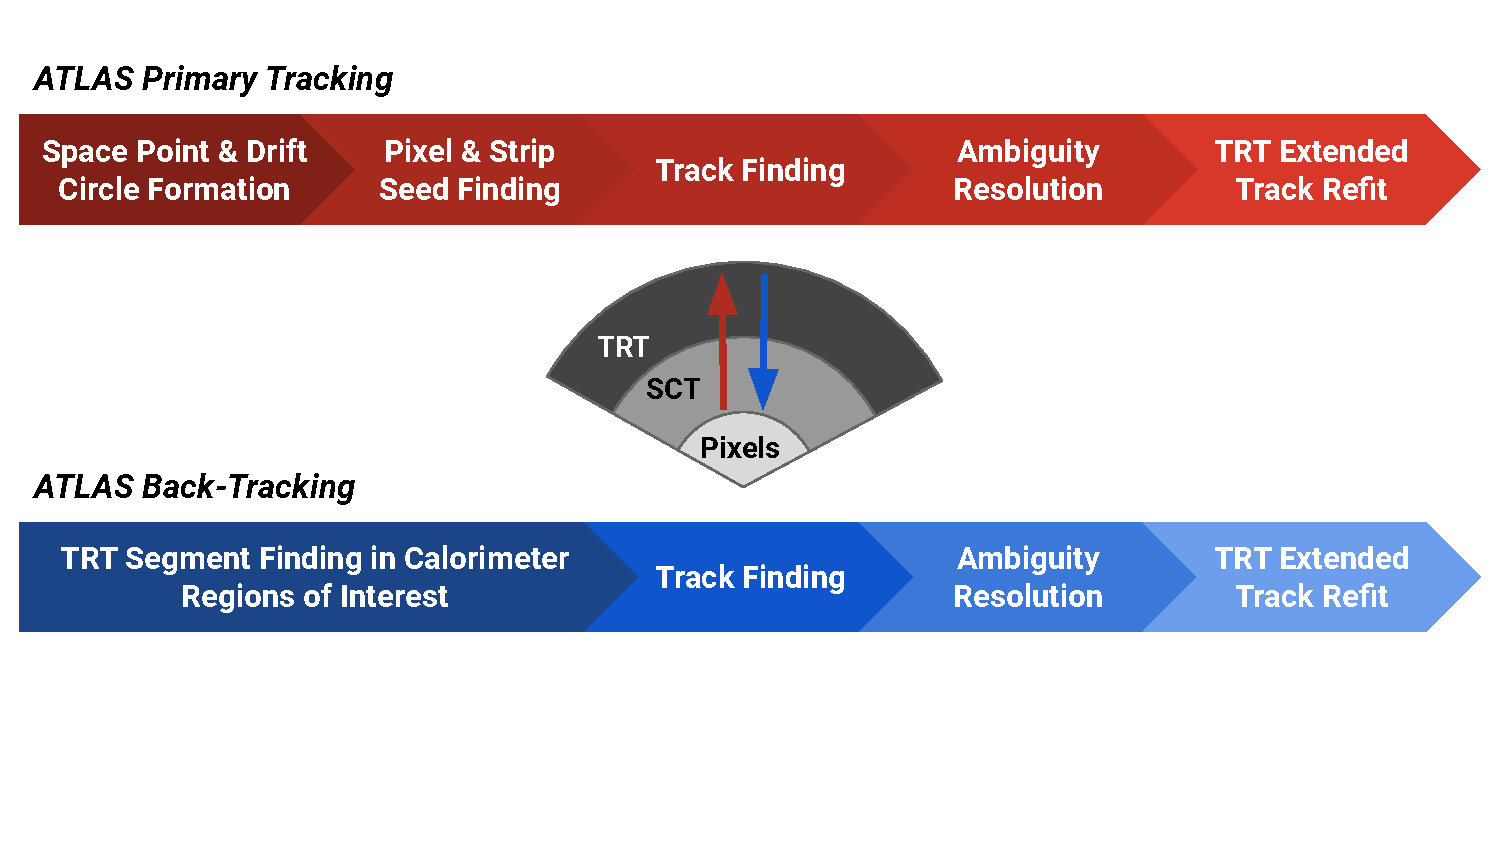
\includegraphics[width=0.8\linewidth]{plots/atlas/outin_tracking.pdf}
%    \caption{Illustration of primary and secondary tracking chains using in ATLAS track reconstruction. From \cite{Atlas:trackreco_run3}.\label{fig:outin_tracking}}%consider removing?
%\end{figure}

To increase the acceptance of the tracking to particles produced away from the beamline, such as electrons originating from photon conversions, tracks are reconstructed from the outside-in (seeded by the TRT) using detector hits not already associated with tracks from the primary pass. To avoid large contributions from falsely reconstructed tracks backtracking is only performed in regions seeded by energy deposits (\et > 6 GeV) in the EM calorimeter \cite{Atlas:trackreco_run3}.

With the mean number of interactions per bunch-crossing being $\langle\mu\rangle=33.7$ for Run-2 \cite{Atlas:mu}, precisely identifying the specific $pp$ interactions, called primary vertices \footnote{``Primary'' refers to $pp$ interactions. Secondary vertices are defined as the spatial locations of hadronic interactions from primary ($pp$) collision products. From here on, the term ``vertex'' will be used to refer to a primary vertex \cite{ATLAS:sv}.}, is an important task. An iterative vertex finding algorithm, which takes all tracks as input parameters, is used for vertex reconstruction. %The first vertex is reconstructed using all tracks, and in each subsequent iteration, the vertex position is refined. After the last iteration, tracks that are incompatible with the vertex are returned to the pool of unused tracks, which are then considered as inputs for a new vertex. The end result is a set of three-dimensional vertex positions and their covariance matrices.
The hard-scatter vertex is usually identified amongst many pileup vertices as the vertex which has the largest $\sum\pt^2$ of contributing tracks. The assumption here is that the charged particles produced in the hard-scatter interaction have a harder \pt spectrum than those produced in pile-up interactions \cite{Atlas:trackreco_run3, Atlas:pvreco}.

\subsubsection{Electrons and Photons}\label{sec:egamma}
Electrons and photons can be identified by the presence of a shower in the EM calorimeter. The showers of electrons and photons are almost indistinguishable, since electrons emit photons through bremsstrahlung, and photons produce electron-positron pairs. However, since the ID only responds to charged particles, photons and electrons can be distinguished through the presence or absence of a track.

Electrons are experimentally defined as objects consisting of a cluster built from energy deposits in the calorimeters and one or more matched tracks. Converted photons are defined as calorimeter clusters matched to a photon conversion vertex. Unconverted photons are defined as clusters without either a matched conversion vertices or an electron track. 

Electron and photon reconstruction starts with a topological cluster (topo-cluster) formation algorithm. Topo-clusters are topologically connected collections of EM and hadronic calorimeter cells, calibrated at the EM scale\footnote{The EM Scale is derived using electron test beams and is defined as the mean calorimeter response measured as the ratio of deposited charge to test-beam energy. The EM scale therefore corrects the measured calorimeter signal to the correct energy for EM showers.}. The algorithm starts with the formation of seed cells, which are required to have a cell energy of at least four times the expected cell noise. Neighbouring cells are then connected if the cell energies are at least twice the expected cell noise. These clusters of cells then go on to become the seed cells for the next iteration, and proto-clusters are merged if they share cells. In the final splitting step, proto-clusters are split into separate clusters if they contain two or more local maxima ($E_{\text{cell}}>500\MeV$ and $\geq4$ neighbours with a smaller signal).

Topo-clusters contain both EM and hadronic calorimeter cells, however, only the energy measured from cells in the EM calorimeter are used for photon and electron reconstruction. Energy measurements in the hadronic calorimeter are still important, however, since they are used to quantify the fraction of the EM calorimeter energy to the total cluster energy, $\mathit{f}_{\text{EM}}$. Topo-clusters with $\mathit{f}_{\text{EM}} > 0.5$ are called EM topo-clusters. Each topo-cluster is interpreted as a massless pseudo-particle, and the energy and momentum components are calculated from the cluster energy at the EM scale and the angular coordinates of the cluster. The reason for defining clusters as massless is because there is no physically meaningful mass without a corresponding particle hypothesis for the origin of the signal \cite{Atlas:topoclusters}. The reconstruction is finalised with the matching of tracks and conversion vertices to clusters using a $\Delta R$ criteria \cite{Atlas:egam_reco}.
%\newline
%A track is considered matched to a topo-cluster if there is small $\Delta\eta$, and a small $\Delta\phi$ separation between the track and the cluster. There is a similar requirement to match conversion vertices to topo-clusters. After matching tracks to topo-clusters, electron and photon ``superclusters'' are seeded from topo-clusters. Superclusters are dynamic, variable sized clusters of calorimeter cells. To build the superclusters, EM topo-clusters are sorted in descending \et. For a cluster to become an electron seed, it must have $\et>1\GeV$, and it must be matched to a track with at least four hits in the Pixel + SCT detectors. For photons, the seed energy threshold is $\et>1.5\GeV$. To capture EM showers originating from the same initial electron or photon, ``satellite'' clusters are identified using an $\eta-\phi$ window of size $0.075\times0.125$ around the centre of the seed cluster. For electrons, a secondary cluster is also considered a satellite if it shares the same best-matched track with the seed, and the secondary cluster is within a larger $\eta-\phi$ window of size $0.125\times0.300$. For converted photons, secondary clusters are considered satellites if they share the same conversion vertex, or if the secondary cluster is matched to a track that belongs to the conversion vertex. The seed clusters and their associated satellites are called superclusters. After this, tracks and conversion vertices are matched to superclusters, and there is an additional ambiguity resolution step to resolve cases where a given seed produces both an electron and a photon. The ambiguity is either resolved or these objects are explicitly marked as ambiguous. The reason for using superclusters as opposed to fixed-sized clusters (fixed-sized clusters were used for early run-2 analyses) is the improved energy resolution, especially in the forward detector regions for electrons and converted photons. In these cases, the improvements can be as large as 40\%.\cite{Atlas:egam_reco} 
%\newline

After reconstruction, electrons and photons are calibrated to account for energy losses in material upstream of the calorimeter, energy deposited outside of the clusters, and energy losses beyond the EM calorimeter. The electron/photon energy scale\footnote{The energy scale is numerical factor that corrects the measured energy to that of simulated truth particles as a function of $\eta$ and \et or \pt.} is determined in a calibration chain, where the response of electrons and photons is derived from simulated samples \cite{Atlas:egamcal_run2,Atlas:egamcal_run1}. After the simulation-based correction is applied, additional corrections are derived using data to account for response variations not included in simulation, and non-linear behaviour of the electronics \cite{Atlas:egamcal_fullrun2}. Finally, a residual energy scale correction factor, called the in-situ calibration, is applied to data so that it agrees with the expectation from simulation. Additionally, a correction factor is applied to simulation so that the energy resolution agrees between data and simulation. These factor are derived using the $m_{ee}$ invariant mass distribution in $Z\rightarrow ee$ events, where a $\chi^2$ minimisation simultaneously solves for the energy scale and resolution parameters in bins of $\eta$. For photons, there is an additional correction to account for the mis-modelling of out-of-cluster leakage. This is only derived for photons since the mis-modelling is found to be lower than 0.1\% for electrons. The photon energy scale calibration is cross-checked using $Z\rightarrow ee\gamma$ decays, and the electron energy scale is validated with $J/\psi(c\bar{c})\rightarrow ee$ events in data \cite{Atlas:egamcal_run1,Atlas:egamcal_fullrun2}. The calibration chain used for correcting the full 140\infb Run-2 dataset is shown as a schematic in Figure \ref{fig:atlas_egamcali}.

\begin{figure}[t]
    \centering
    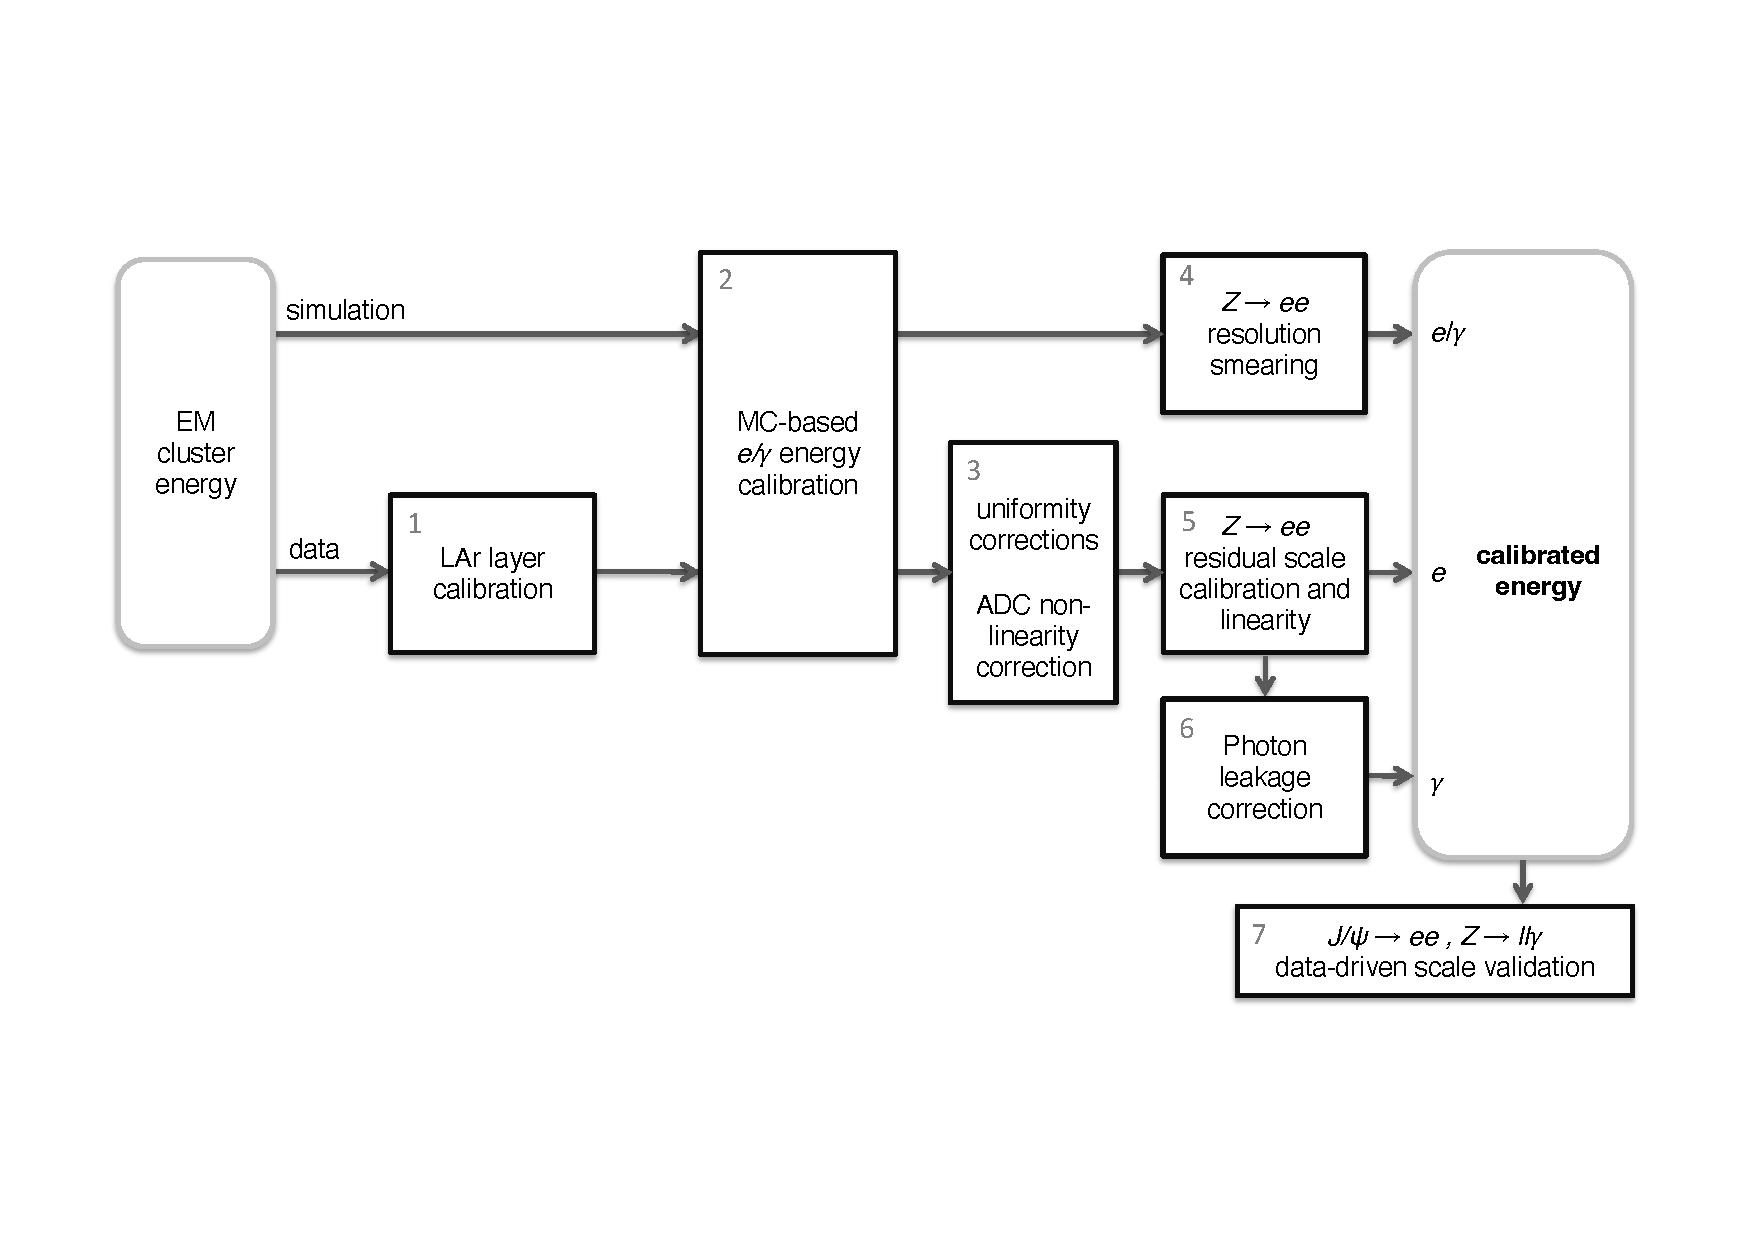
\includegraphics[width=\textwidth]{plots/atlas/egammacali.pdf}
    \caption{The $e/\gamma$ calibration chain used to correct the full Run-2 ATLAS dataset. Figure from \cite{Atlas:egamcal_fullrun2}.\label{fig:atlas_egamcali}}
\end{figure}
Electrons and photons can be mimicked by other objects, particularly jets, converted photons and heavy-flavour hadron decays. It is actually very rare for a jet to be collimated in addition to being almost entirely contained in the EM calorimeter \cite{Atlas:egamcal_run2}. After reconstruction and calibration, identification algorithms based on shower shape variables are calculated to separate prompt\footnote{The definition of a prompt lepton are those not from hadron decays. Prompt photons are those not from hadron or $\tau$ lepton decays \cite{Atlas:truthdefs}.} electron/photons from jets. These variables quantify the degree to which the shower is collimated (the lateral shower development), how deep the shower penetrates the calorimeters (the longitudinal shower development), and in the case of electrons, the spatial compatibility of the track with the cluster.

Prompt electrons entering the central region ($|\eta|<2.47$) of the detector are selected using a likelihood-based (LH) identification (ID) discriminant \cite{Atlas:egam_reco}. By cutting on values of this discriminant, a given electron candidate can pass or fail \textit{Tight}, \textit{Medium}, \textit{Loose}, or \textit{VeryLoose} ID criteria. An electron satisfying a tighter working point has lower reconstruction efficiency but is more likely to correspond to a prompt electron. The likelihood discriminant is determined from signal and background probability density functions (pdf\footnote{pdf refers to probability density function, and PDF (capitalised) refers to parton distribution function.}). The signal pdfs are derived from $Z\rightarrow ee$ and $J/\psi\rightarrow ee$ events with a strict requirement on one of the reconstructed electrons and a very loose requirement on the other electron. The background pdfs are derived in a dijet enriched, prompt electron deficient fiducial region.

For photon identification within the region of $|\eta|<2.37, 1.37 < |\eta| < 1.52$ excluded, a cut-based, selection is implemented. Photon ID criteria are designed to select prompt, isolated photons, and reject backgrounds from jets. Eleven shower shape variables are used to define \textit{Tight}, \textit{Medium}, and \textit{Loose} (the latter two are used in the trigger) working points. Additionally, there are multiple photon ID working points for variations of the \textit{Tight} selection, where a number of shower-shape variable cuts have either been removed, or relaxed. These are called \textit{LoosePrime2-5}. These working points are useful for estimating systematic uncertainties on non-prompt photon estimates \cite{Atlas:egam_reco,Atlas:egamcal_run2}. 

The degree to which reconstructed electrons or photons are surrounded by other particles can be quantified using calorimeter or track based isolation variables. The calorimeter-based isolation energy ($E_{\text{T}}^{\text{coneXX}}$) is calculated by summing up the energy of topo-clusters whose barycentre\footnote{The barycentre of a topo-cluster is the average position of the cluster, weighted by energy deposits.} falls within a fixed-size cone of size $\Delta R$ of the EM particle cluster barycentre ($E_{\text{T,raw}}^{\text{isolXX}}$), and subtracting the energy contributed by the electron or photon which is taken to be a fixed $\Delta\eta\times\Delta\phi=5\times7$ cluster around the barycentre of the EM particle cluster ($E_{\text{T,core}}$). An additional leakage correction ($E_{\text{T,leakage}}$) is required to account for the fact that not all of the EM particle energy is subtracted. Finally, there is a correction to account for pileup and underlying-event\footnote{The underlying event (UE) is usually defined as all particles from a single particle collision except those from the process of interest. The UE is not equivalent to minimum bias events, but they are related \cite{Atlas:ue}.} ($E_{\text{T,pile-up}}$). The full calorimeter-based isolation energy is expressed as:
\begin{equation}
    E_{\text{T}}^{\text{coneXX}}=E_{\text{T,raw}}^{\text{isolXX}}-E_{\text{T,core}}-E_{\text{T,leakage}}(E_{\text{T}},\eta,\Delta R)-E_{\text{T,pile-up}}(\eta,\Delta R),
\end{equation}
where XX refers to the size of the cone, $\Delta R=\text{XX}/100$. The track isolation variable ($p_{\text{T}}^{\text{coneXX}}$) is calculated by summing the \pt of tracks within a cone centered around the electron track or photon cluster direction, whilst excluding the tracks matched to the electron or converted photon. Track-based isolation has better resolution and lower pile-up dependence and provides a superior \pt resolution. However, calorimeter-based isolation includes neutral particles and particles below the ID track \pt threshold. Hence, both variables provide complimentary information, and the combination of selections on both variables generally results in improved performance over cutting on one variable \cite{Atlas:egam_reco}.

Electron isolation working points include the \textit{Gradient} working point which is defined such that the selection efficiency is $95\%$ at $\pt = 20\GeV$ and $99\%$ at $\pt = 60\GeV$, as well as \textit{Loose}, \textit{Tight}, and \textit{HighPtCaloOnly} which implement a cut on the calorimeter or track isolation variables as a function of \pt. The \textit{HighPtCaloOnly} working point gives the largest rejection of all the working points at high \pt, and only uses the calorimeter-based isolation variable. There are three photon isolation working points: \textit{Loose}, \textit{Tight}, and \textit{TightCaloOnly}. These all cut on the isolation variables as a function of \et, and the \textit{TightCaloOnly} working point only uses the calorimeter-based isolation variable. 

Differences between data and simulation can arise due to imperfect detector modelling (see Section \ref{sec:dataproc} for more details), mismodelling of the shower shape variables, as well as the modelling of complex objects such as the beamspot. The ratios of the data-to-MC efficiencies are referred to as ID or isolation efficiency scale factors, or just scale factors, and correct the MC simulations so that they closely resemble the data. Systematic variations in these scale factors are propagated through to the analysis-level objects \cite{Atlas:photonid_run2}.

%TODO: Define barycentre and the likelihood discriminant

%These variables capture things like ratios of energy deposited in a particular layer of the calorimeter relative to that deposited in another layer or relative to the total cluster energy, as well as lateral shower widths.
%Could mention improved energy resolution that superclusters provide (presumably over old sliding window algorithms?). Width quantified using inter-quartile-range, IQE.
%Discuss electron and photon energy calibration next. After the calibration, the shower shape variables and other discriminating variables are calculated for electron and photon ID.

\subsubsection{Muons\label{sec:muon}}
 
Muons can be reconstructed solely using the MS (stand-alone muons), or a combination of detector subsystems. Stand-alone muons are of use in the reconstruction of ID + MS combined muons and when operating in the forward region $2.5 < |\eta| < 2.7$, which is not covered by the ID. Stand-alone muon reconstruction starts with track reconstruction in the MS, where preliminary track candidates are formed through the identification of short straight-line track segments from hits in individual MS stations. The tracks are then built using all MS subdetectors, taking into account detector-misalignment, particle-detector interactions, outlier hits, track overlaps, and calorimeter energy losses. Track candidates are finalised after being extrapolated to the IP \cite{Atlas:muonreco}.%precision three-dimensional track coordinates are constructed using information from all of the MS subdetectors. Muon trajectories are built with a global $\chi^2$ fit which takes detector misalignment and particle-detector interactions into account. In the next step, these trajectories have outlier hits removed, and hits compatible with the trajectory which were not originally assigned are added. The tracks are then refit with this updated information. In an ambiguity resolution step lower quality tracks are removed if they have a large overlap with high quality tracks. The final tracks are then refit with a loose IP constraint, taking energy losses in the calorimeters into account, and the tracks are extrapolated to the beam line.

In most cases, it is advantageous to combine the signals from the MS with other detector subsystems. Since muons are the only standard model particle that leave signatures in the MS, usually the combination of ID and MS information is sufficient. However, in some special cases it is advantageous for the full detector information to be used. There are four classes of reconstructed muons where detector information beyond the MS is used:
\begin{enumerate}
    \item Combined muon (CB) tracks are formed from a successful combination of stand-alone MS muons and ID tracks.
    \item Inside-out combined (IO) muons are reconstructed with an algorithm that extrapolates ID tracks to the MS whilst using the ID track, the calorimeter energy losses, and the MS hits in a combined fit. IO muons have some performance improvements over CB muons as they do not rely on the independently reconstructed MS track. Most analyses only select for combined (either CB or IO) muons as the combination of two tracks results in the best possible precision.
    \item Segment Tagged (ST) muons are required to have a tight angular matching of an ID track to at least one reconstructed MS segment, and the muon parameters are taken solely from the ID track fit. ST muons are of use when there is no fully reconstructed MS track, but only segments in layers of the MS. This can be the case with low \pt muons.
    \item Calorimeter-tagged (CT) muons require an ID track which is extrapolated into the calorimeters. Energy deposits compatible with a minimum ionising particle are used to tag the ID track as a muon, and the muon parameters are taken directly from the ID fit. CT muons are only of use when there is no MS track, which is possible for cases where there are known holes in the MS. The signatures for these muons are easily caused by other particles and hence CT muons have low purity (one minus hadron misidentification rate).
\end{enumerate}
Muon identification working points (\textit{Loose}, \textit{Medium}, and \textit{Tight}) are defined to moderate the prompt muon purity and reconstruction efficiency trade-off. This is achieved through requirements on the number of hits in ID layers and MS stations, track properties, and ID-MS compatibility variables. Non-prompt muons can come about due to semileptonic decays of light hadrons as well as heavy-flavour hadron decays. Since light hadron decays result in lower-quality muons, the working points are optimised to reject muons from light-flavour hadrons. Non-prompt muons from heavy flavour decays result in higher quality muon tracks and can usually therefore be distinguished from prompt muons through the association with the primary vertex and the isolation of the ID tracks or calorimeter deposits. In addition to the standard working points, \textit{Low-}\pt and \textit{High-}\pt working points are optimised to select for low and high \pt muons.

The track and calorimeter-based isolation variables for muons are defined in a similar way to electrons and photons (Section \ref{sec:egamma}). \pt requirements on the calorimeter and track-based isolation variables as well as a requirement on the track \pt give an array of isolation working points. These are \textit{Loose} and \textit{Tight}, in addition to more specialised working points such as the \textit{particle-flow} working points which are optimised to reject muons from heavy-flavour hadrons, as well as a set of track-only working points \cite{Buckley:PCP,Atlas:muonreco}.

\subsubsection{Jets\label{sec:atlas:jets}}
%The vast majority of $pp$ collisions at the LHC result in the production of quarks and gluons of which the observable signatures are collimated streams of hadrons, \textit{jets}. A number of algorithms for the clustering of observed detector outputs into jet objects exist, of which the primary one for ATLAS jet reconstruction is the anti-$k_t$ algorithm (Section \ref{sec:theory:jet}) with a distance parameter $R=0.4$. Four-momentum vector \textit{input objects} form the inputs to the algorithm, which may be derived from various sources. These are either tracks, calorimeter deposits organised into topo-clusters, or a combination of track and calorimeter information. The most common anti-$k_t$ distance parameter is $R=0.4$ (small-R jets), however, jets reconstructed with $R=1.0$ (large-R jets) are used in cases where high \pt jets originate from the hadronic decays of massive particles like H/W/Z bosons and top quarks. Since the angular separation of their decay products scales as $1/\pt$, i.e. $\Delta R\approx\frac{2m}{\pt}$, they become collimated (highly Lorentz-boosted) \cite{Atlas:altinputsjetgrooming}. In these situations, these decay products can be reconstructed in a single large-R jet.
The vast majority of $pp$ collisions at the LHC result in the production of quarks and gluons of which the observable signatures are collimated streams of hadrons, \textit{jets}. A number of algorithms for the clustering of observed detector outputs into jet objects exist, where the primary one for ATLAS jet reconstruction is the anti-$k_t$ algorithm (Section \ref{sec:theory:jet}). The most common anti-$k_t$ distance parameter is $R=0.4$ (small-R jets), however, jets reconstructed with $R=1.0$ (large-R jets) are used in cases where high \pt jets originate from the hadronic decays of massive particles like H/W/Z bosons and top quarks. Since the angular separation of their decay products scales as $1/\pt$, i.e. $\Delta R\approx\frac{2m}{\pt}$, they become collimated (highly Lorentz-boosted) \cite{Atlas:altinputsjetgrooming}. In these situations, these decay products can be reconstructed in a single large-R jet.

The inputs to the anti-$k_t$ algorithm are four-momentum vectors called \textit{input objects}, which can be derived from various sources. These are either tracks, calorimeter deposits organised into topo-clusters, or a combination of track and calorimeter information. Jets reconstructed solely from tracks are referred to as \textit{track-jets}. The acceptance limitations of the ID ($|\eta|<2.5$), and the inability for the ID to measure neutral particles limits the usefulness of track-jets. For this reason, jets in most ATLAS analyses are reconstructed solely using calorimeter topo-clusters, or a combination of topo-clusters and tracks. 
%Put this a bit later: At the heart of PFlow algorithms is the ability to distinguish the calorimeter energy deposits of neutral particles from charged particles. 
%\footnote{Athena is the name of the ATLAS software framework that manages almost all ATLAS production workflows including event generation, simulation, reconstruction and derivation production. All the work in this thesis uses Athena release 21, which was the release for run-2 data taking. Release 22 was used in initial run-3 data taking and is used in newer analyses for the reprocessing of run-2 data} 
% First year report

The formation of topo-clusters for jet reconstruction is identical to the description given in Section \ref{sec:egamma}. Calorimeter jets reconstructed at the EM scale are called \textit{EMTopo jets}. Calorimeter jets can also be reconstructed at the \textit{Local hadronic Cell-Weighting} (LC) scale, where an additional calibration factor is applied to topo-clusters consistent with hadronic energy deposits. These jets are called \textit{LCTopo} jets. The LC weighting is derived from simulations of single pion events, and corrects for signal losses and calorimeter non-compensation.

%It worth pointing out that further work is required to combine LC weighting with PFlow algorithms. Therefore, only jets reconstructed solely from calorimeter deposits are currently calibrated with the additional LC weighting
In Run-1 and in early Run-2 analyses, jets were reconstructed solely using topo-clusters. However, using a combination of ID and calorimeter information is preferable for the reasons that:
\begin{itemize}
    \item The calorimeters provide measurements of both charged and neutral particles.
    \item The superior angular resolution of the ID means that tracks can be associated with vertices.
    \item The momentum resolution of the ID at low \et is superior to that of the calorimeters. 
    \item The energy resolution of the calorimeters at high \et is superior to that of the ID.
    \item The calorimeters cover the forward $2.5<|\eta|<4.9$ regions.
\end{itemize}

%\subsubsection{The PFlow algorithm}
%
Different algorithms are used for the complimentary use of both track and calorimeter information. These algorithms are classified under the umbrella term of \textit{particle-flow}, or PFlow, algorithms \cite{Atlas:PFlowOG}\footnote{In this thesis, the terms \textit{particle/PFlow jets} and \textit{\textbf{the} particle/PFlow algorithm} will be used to refer to the particle flow algorithm described in \cite{Atlas:PFlow}. However, particle flow is a broader concept which can also be used to describe other input object algorithms. These are the TCC and UFO algorithms, and are described further on in this chapter.}. The PFlow algorithm described in \cite{Atlas:PFlow} was developed at ATLAS to combine tracking and calorimetric information for hadronic jet and soft activity\footnote{Soft activity is the additional hadronic recoil below the energy threshold used for jet reconstruction (this is important for missing transverse momentum reconstruction).} reconstruction. At the heart of this algorithm is the ability to distinguish charged from neutral particle deposits in the calorimeters and furthermore to subtract the energy deposited by charged particles from the topo-clusters and to replace them with the momenta of tracks matched to the topo-clusters. The output of the algorithm is a list of tracks, a list of unmodified topo-clusters, and a list of modified topo-clusters. These outputs are often referred to as a Particle Flow Objects (PFOs). The pion mass is assumed, since pions dominate the charged component of the jet, and to take up an average of approximately two-thirds of the visible jet energy \cite{Atlas:PFlow,Atlas:jetconstituent1,Atlas:jetconstituent2}. %Next, read through page 9-10 of pflow algorithm, decide which parts of that to add, maybe add the flow chart. Decide on which bits to elaborate on further. Maybe don't spend tooooo much time on PFlow stuff. Still need UFO, TCC, JER, JMR, calibration, Insitu. 

The steps of the PFlow algorithm are as follows:
\begin{enumerate}
    \item \textbf{Track selection}: Well-measured tracks are selected: 9 hits in the Pixel + SCT; no pixel holes; ID acceptance $|\eta|<2.5$; and $0.5\GeV<\pt<40\GeV$. The lower bound \pt threshold is chosen to allow for tracks from particles below the topo-cluster energy threshold. The upper bound selects against poorly isolated tracks. Tracks matched to electrons or muons with \textit{medium} ID are rejected since the algorithm is optimised for hadronic showers.
    \item \textbf{Matching tracks to topo-clusters}: For each track, an attempt is made to find a match with a single topo-cluster. In some cases tracks are determined to not have formed a topo-cluster. These tracks are retained in the algorithm output list of tracks and steps 3-6 are not performed.
    \item \textbf{Expected deposited particle energy}: The mean deposited energy of a track of measured momentum $p^{\text{trk}}$, denoted $\langle E_{\text{dep}}\rangle$, is determined using single-pion samples without pileup. Additionally, the spread in the expected single-pion energy deposition ($\sigma(E_{\text{dep}})$) is determined. These are important quantities for steps 4-6 of the algorithm. 
    \item \textbf{Split-shower recovery}: For each track/topo-cluster system, a discriminant $S(E^{\text{clus}})\equiv\frac{E^{\text{clus}}-\langle E_{\text{dep}}\rangle}{\sigma(E_{\text{dep}})}$, where $E^{\text{clus}}$ is the energy of the topo-cluster, is calculated to distinguish between cases where the particle energy is entirely deposited in a single topological cluster, and cases where the energy is split across multiple topo-clusters. This is actually very common, especially where the shower is split across two topo-clusters. A value of $E^{\text{clus}}>-1$ indicates that more than 90\% of clusters have the large majority ($>90\%$) of the particle's true energy deposited in the topo-cluster. Hence a discriminant value of $-1$ is used in performing the split-cluster recovery. The algorithm extrapolates the track to the EM calorimeter and expands the set of matched clusters using a simple $\DeltaR=0.2$ criteria around the extrapolated track.
    \item \textbf{Cell-by-cell subtraction}: It is possible that particles unrelated to the track (for example neutral particles) deposit their energy in close proximity to the clusters matched to the track. Hence simply removing every topo-cluster matched to a track would potentially remove energy deposits made these close-by particles. For this reason, the energy of the total set of topo-clusters is compared to $\langle E_{\text{dep}}\rangle$, and if it is less than $\langle E_{\text{dep}}\rangle$, the topo-clusters are removed. If total topo-cluster energy is larger than $\langle E_{\text{dep}}\rangle$, a cell-by-cell subtraction procedure is implemented to remove calorimeter cells around the extrapolated track.%$33.2\times\text{log}_{10}(40\GeV/{\pt^{\text{trk}}})$
    \item \textbf{Remnant removal}: If the cell-by-cell subtraction is implemented, it is likely that there will be some remaining energy from the cells that were not subtracted (if there are energy deposits from neutral particles, for example). A procedure is implemented to determine whether this energy is consistent with shower fluctuations, or whether the energy is consistent with close-proximity particle deposit(s). The remnant topo-clusters are removed if the former case, and retained in the latter.
\end{enumerate}
Figure \ref{fig:pflow} shows a flow chart of this PFlow algorithm.
\begin{figure}[t]
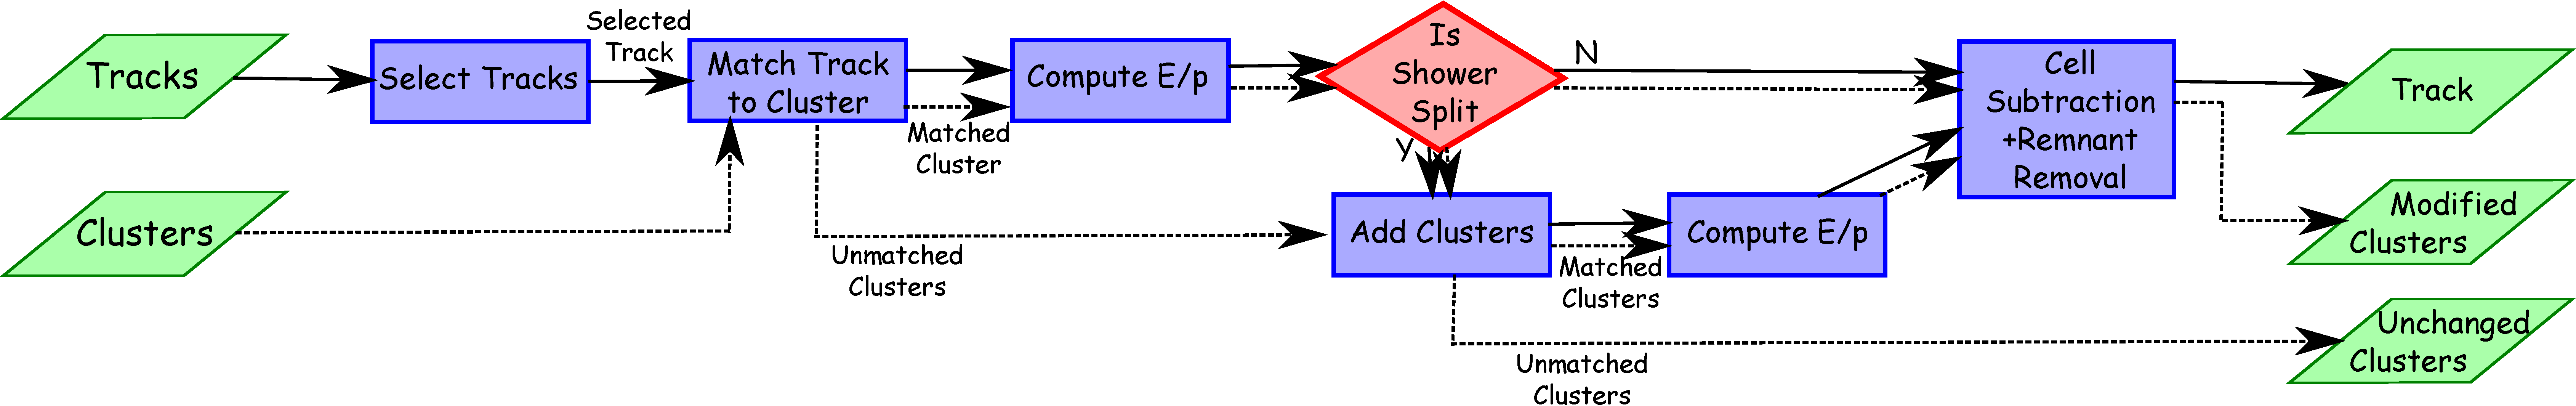
\includegraphics[width=\textwidth]{plots/atlas/pflow.pdf}
\caption{Flow chart showing the algorithm used in the construction of particle flow jet input objects. Figure from \cite{Atlas:PFlow}.\label{fig:pflow}}
\end{figure}

In the presence of pileup, where jets can arise from particles not produced in the primary hard scatter interaction, the performance benefits of PFlow jets can clearly be observed. This is shown in Figure \ref{fig:pflow_perf:a}, where the average number of pileup jets (referred to a ``fake jets'' in the figure) are compared between LCTopo jets and PFlow jets. The fake-rate is an order of magnitude lower for PFlow jets in the region of tracker acceptance, and there are no large deviations in performance outside of the tracker acceptance. Figure \ref{fig:pflow_perf:b} shows the efficiency of reconstructing a hard-scatter jet, and improvements to the hard-scatter jet reconstruction efficiency can be seen in the comparison of PFlow jets to LCTopo jets. 
\begin{figure}[t]
\centering
\begin{subfigure}[b]{0.46\textwidth}
    \centering
    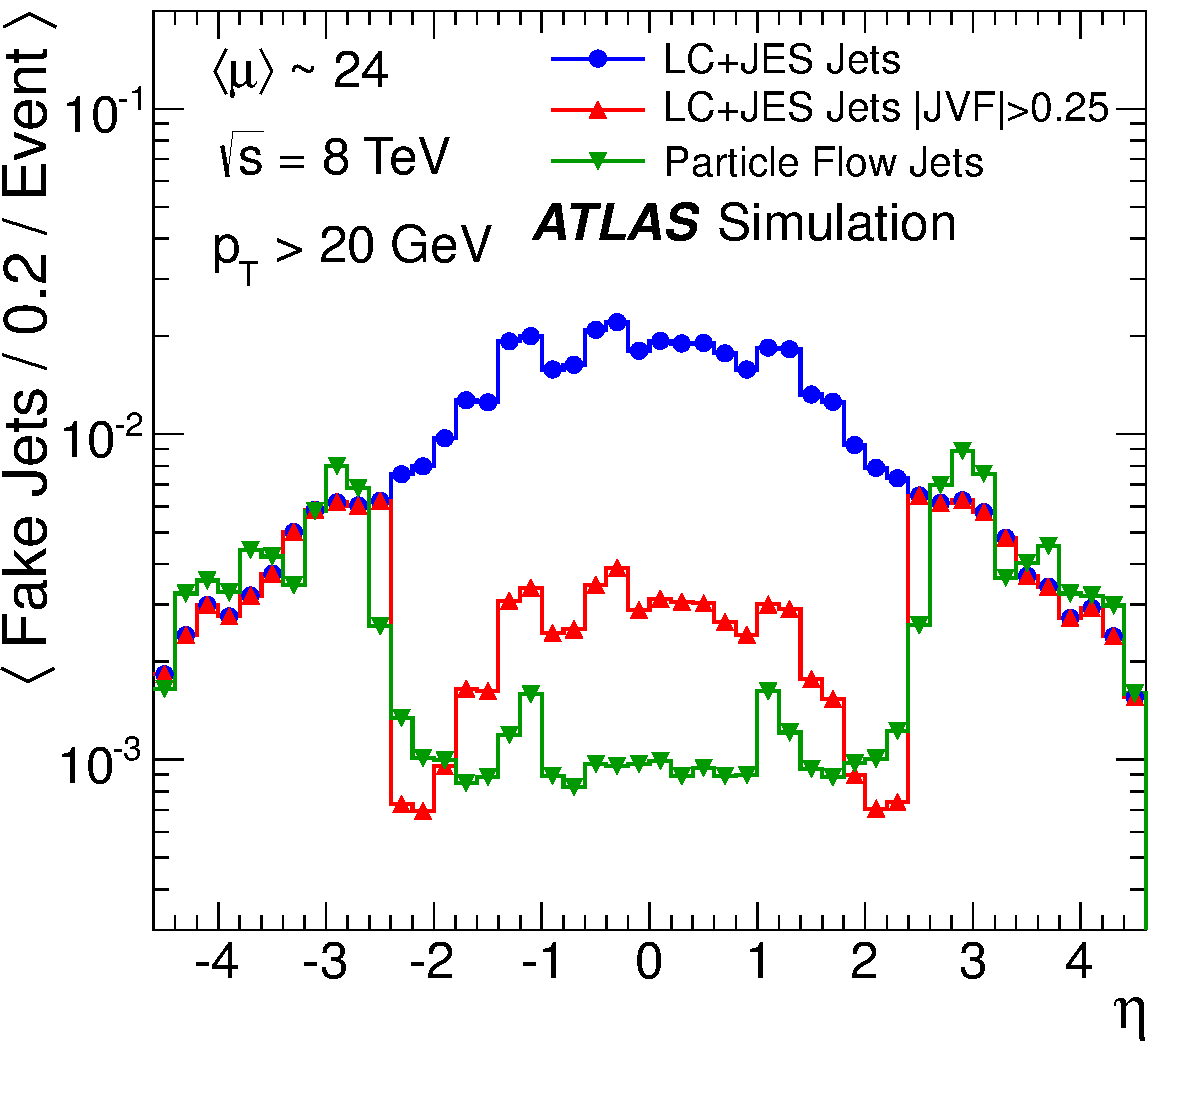
\includegraphics[width=\textwidth]{plots/atlas/pflow_performance_a.pdf}
    \caption{}
    \label{fig:pflow_perf:a}
\end{subfigure}
\hfill
\begin{subfigure}[b]{0.46\textwidth}
    \centering
    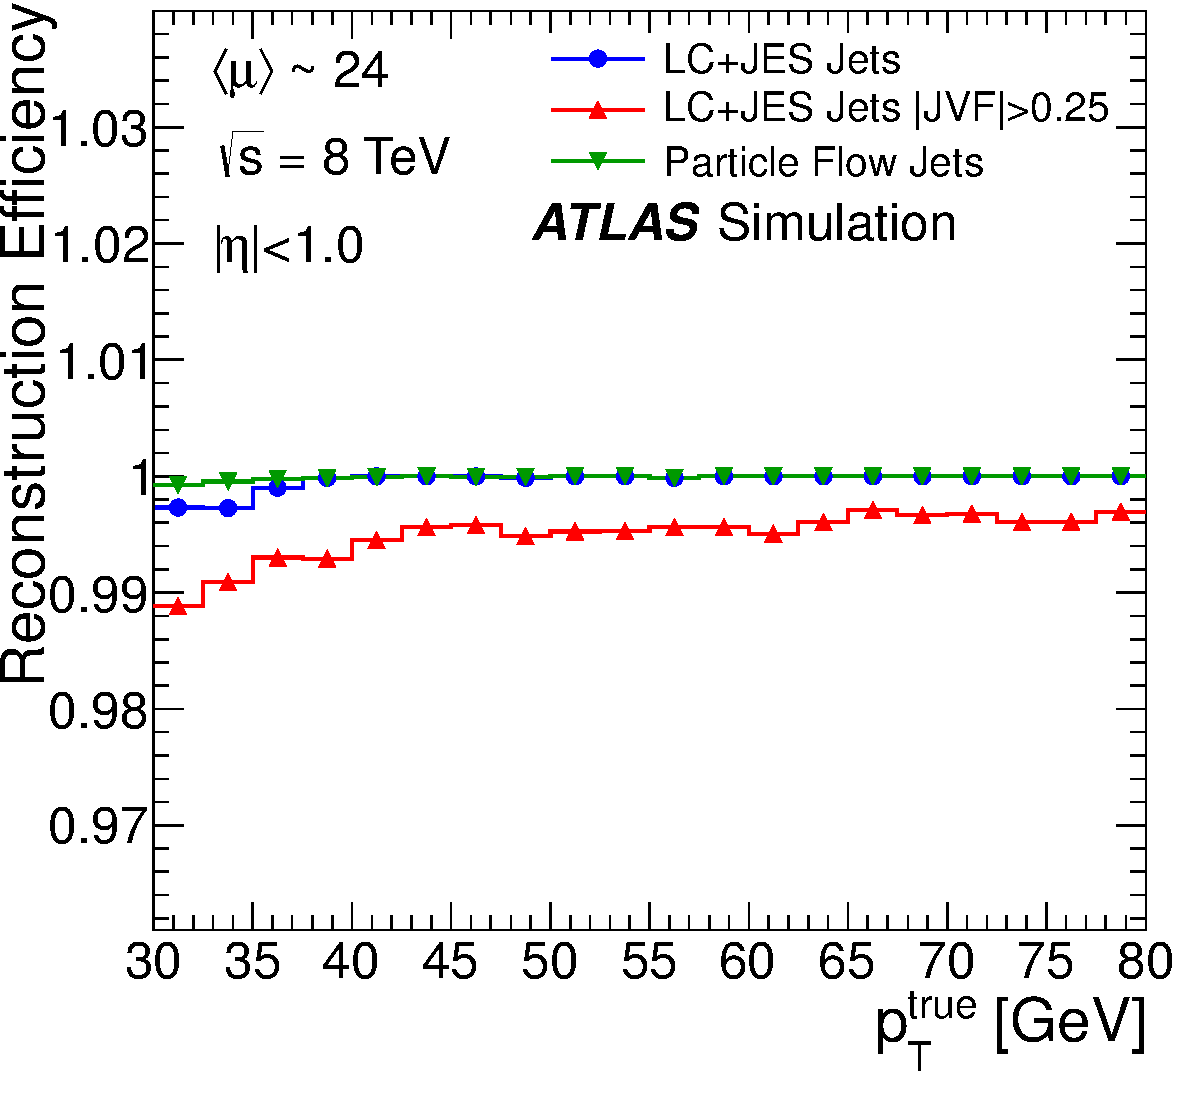
\includegraphics[width=\textwidth]{plots/atlas/pflow_performance_b.pdf}
    \caption{}
    \label{fig:pflow_perf:b}
\end{subfigure}
\caption{Performance improvements of PFlow jets over calorimeter jets. Figures from \cite{Atlas:PFlow}. with and without a jet vertex fraction (JVF) cut applied. JVF is the ratio of two scalar sums, where the numerator is the scalar sum of the \pt of tracks associated to the jets which are matched to the the hard-scatter vertex; and the denominator is the scalar sum of \pt of all tracks associated with the jet. \label{fig:pflow_perf}}
\end{figure}

In spite of the performance benefits shown in Figure \ref{fig:pflow_perf}, the algorithm does have some shortcomings, particularly at high \pt. Since the lateral shower width of a jet scales as 1/\pt, high \pt jets have a dense core. The presence of a dense core degrades the accuracy and efficiency of track reconstruction. Additionally, the angular resolution of the calorimeter limits the degree to which the cell subtraction step can be performed reliably in the presence of close proximity showers. It is because of these reasons, that tracks with $\pt > 40\GeV$ are excluded from the algorithm in the track selection step \cite{Atlas:PFlowOG}. 

%\subsubsection{The TCC algorithm}
Another PFlow algorithm called the Track-CaloCluster (TCC) algorithm \cite{Atlas:TCC} was developed at ATLAS for improved jet substructure reconstruction performance, and hence tagging performance in very high \pt jets. Since the energy resolution of the calorimeters is superior to that of the ID at high \pt, the TCC algorithm directly uses the energy information from topo-clusters and the angular information from tracks. The output of the TCC algorithm is a set of four-momenta (\pt,$\eta$,$\phi$,$m$), where $m$ is the invariant mass of the object\footnote{TCC objects are massless if $\leq 1$ topo-clusters are matched to the seed track, and have non-zero mass if multiple clusters are matched to the seed track}. The TCC algorithm works are follows:
\begin{itemize}
    \item All \textit{loose} tracks matched to primary vertices (including pileup) are matched to topo-clusters calibrated at the LC scale, and each track forms its own TCC object. In cases where one track matches one topo-cluster, the \pt of the TCC object is taken from the topo-cluster, and the $\eta$ and $\phi$ coordinates from the track.
    \item If multiple tracks match to multiple topo-clusters, the cluster \pt is split amongst the tracks, and the track angular coordinates are taken from the seed track.
    \item In cases where there is a topo-cluster (track) unmatched to a track (topo-cluster), the four-momentum of the TCC object is taken as that of the topo-cluster (track).
\end{itemize}
%\subsubsection{The UFO algorithm\label{sec:UFO}}
A particle flow algorithm called the Unified Flow Object (UFO) algorithm was designed as a solution to the problem that no single jet input object definition, be it PFlow, TCC or LC/EMTopo, is optimal for any given measure of performance. TCC jets, while having excellent tagging performance at high \pt, perform worse than LCTopo jets at low \pt. PFlow jets outperform LCTopo jets across the entire \pt range, particularly when it comes to pileup sensitivity. However, PFlow jets have significantly worse tagging performance than TCC jets at high \pt. 

The UFO algorithm combines the PFlow algorithm in \cite{Atlas:PFlow} and the TCC algorithm \cite{Atlas:TCC} in such a way as to optimise the performance across the kinematic range. In this algorithm, the $\pt^{\text{trk}}<40\GeV$ cut is replaced with a method to gradually switch from the PFlow cell subtraction to the TCC cell subtraction depending on $\pt^{\text{trk}}$, and on the measured calorimeter activity \cite{Atlas:PFlow2}. The switch is made if the energy $E^{\text{clus}}$ in a cone of size $\Delta R=0.15$ around the extrapolated particle satisfies:
\begin{equation}
    \frac{E^{\text{clus}}-\langle E_{\text{dep}}\rangle}{\sigma(E_{\text{dep}})}>33.2\times\text{log}_{10}(40\GeV/{\pt^{\text{trk}}}).
    \label{eq:denseenvironment}
\end{equation}
In this way, the PFlow cell subtraction algorithm is not implemented for cases where the track momentum is high, and in cases where the measured calorimeter activity is high, such as in very dense environments. Additionally, charged PFOs (tracks selected by PFlow algorithm) which are not matched to the hard-scatter vertex are removed in order to suppress contributions from pileup. This procedure is called ``Charged Hadron Subtraction'' (CHS). The neutral PFOs (modified or unmodified topo-clusters) have constituent-level (before jet building with anti-$k_t$) pileup mitigation algorithms applied that go by the names of ``Constituent Subtracton'' (CS) and SoftKiller (``SK''). These pileup mitigation algorithms are applied for both small-R and large-R jets. The full UFO algorithm is outlined in Figure \ref{fig:ufoalgorithm}. UFO jets will be the default for small-R and large-R jet definitions in Run-3 analyses.
\begin{figure}[t]
    \centering
    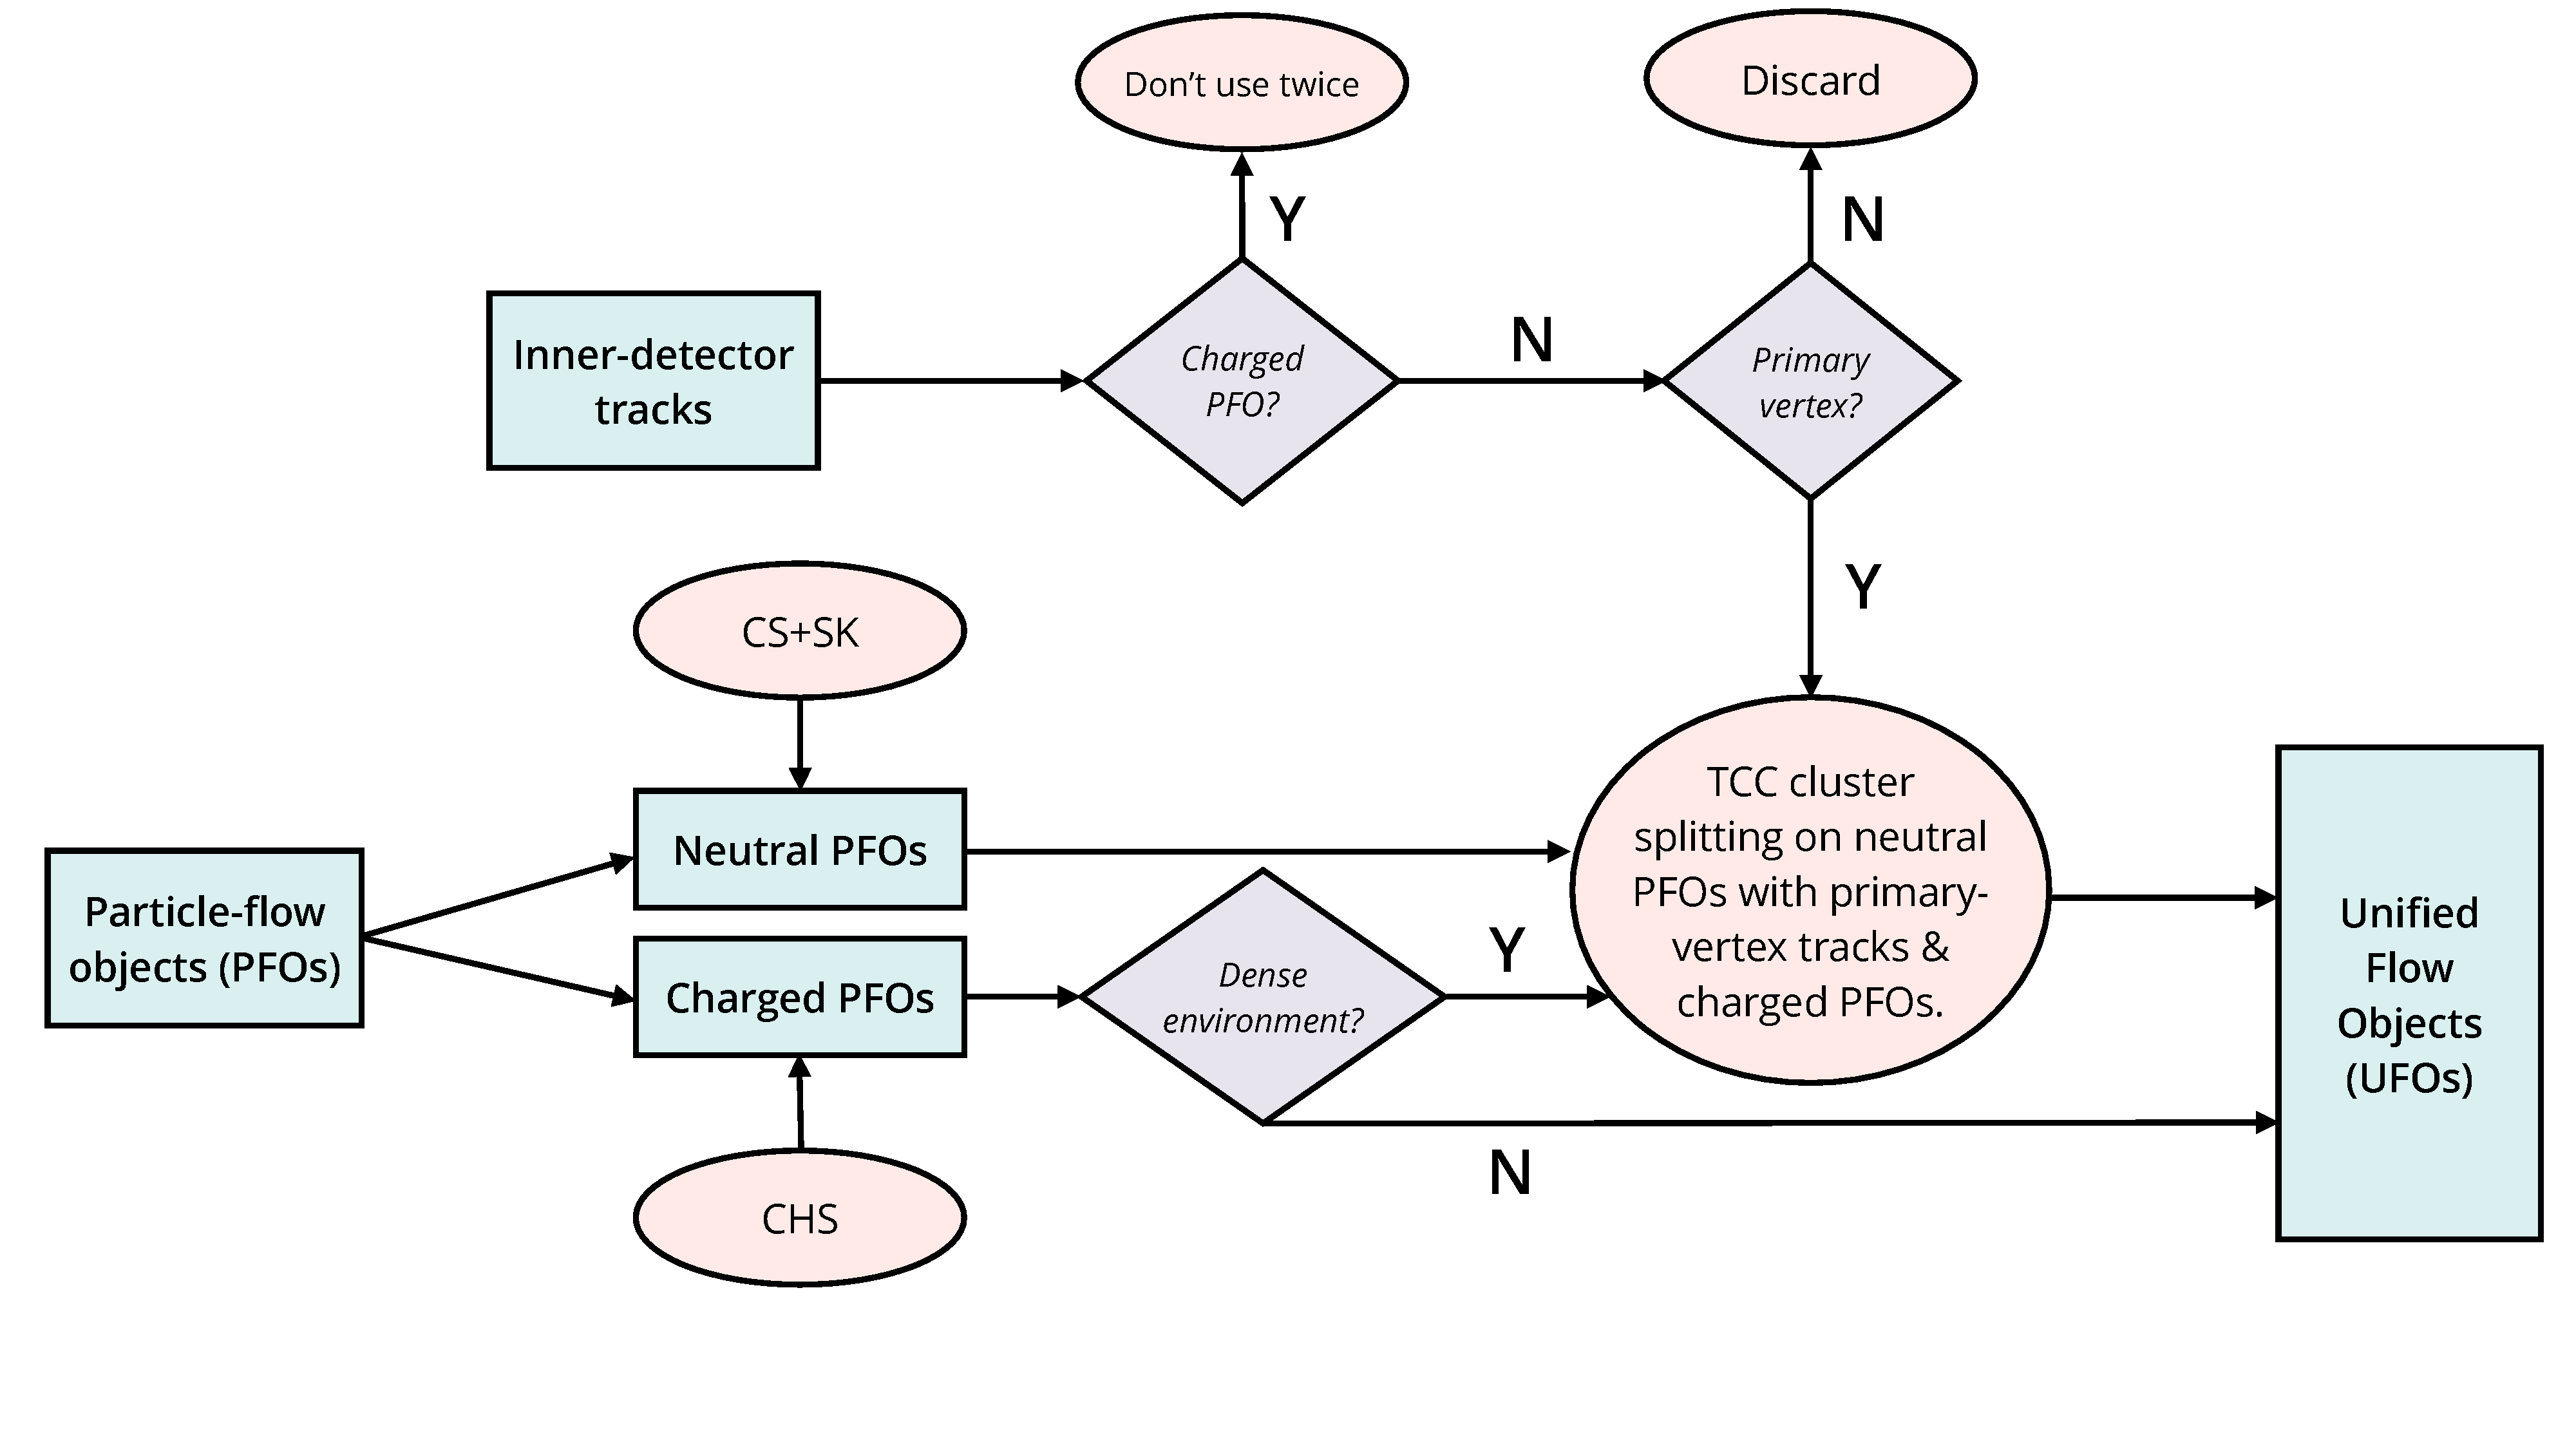
\includegraphics[width=\textwidth]{plots/atlas/ufoalgorithm.pdf}
    \caption{A flow chart outlining the construction of UFO jet input objects from PFOs and ID tracks. The ``dense environment'' decision is defined by equation \ref{eq:denseenvironment}, and results in the TCC algorithm being applied to track and topo-cluster combinations with high \pt tracks or very energy-dense calorimeter environments.\label{fig:ufoalgorithm}}
\end{figure}
%
%\subsubsection{Jet Energy Resolution (JER)}
%Precise knowledge of the JER is particular importance to precision SM measurements involving jets such as processes sensitive to VBS/VBF production, hadronic days of SM particles, in addition to BSM analyses involving jets. The JER is parametrised in form of equation \ref{eq:energyres}, where there is a contribution from a noise term, a stochastic term, and a constant term. The JER is often expressed in terms of \pt, as opposed to energy. Since the noise term is approximately independent of the energy deposited by the jet shower, the relative contribution from the noise term scales as $1/\pt$ and is thus more important at low \pt (below around 30\GeV). At around several hundred $\GeV$, the stochastic term dominates, which scales at $1/\sqrt{\pt}$. The constant term, which represents energy fluctuations that are a constant fraction of the jet \pt dominates above around 400\GeV. In order to measure the JER directly, a dijet momentum balance technique is used. Additionally, the noise term can be estimated directly through measurements of the fluctuations of the calorimeter energy deposits using pileup events from data samples with random unbiased triggers. The combined JER measurement is obtained using a technique similar to the combination of the different in situ JES measurements. The absolute JER uncertainty in the $\eta=0.2$ region as a function of \pt for 2017 data for calibrated PFlow and EMTopo jets is shown in figure \ref{fig:jer:a}. The absolute JER uncertainty with $\eta$ for 30\GeV jets is shown in figure \ref{fig:jer:b} \cite{Atlas:smallrcali}.
%
%\begin{figure}
%\centering
%\begin{subfigure}[b]{0.46\textwidth}
%    \centering
%    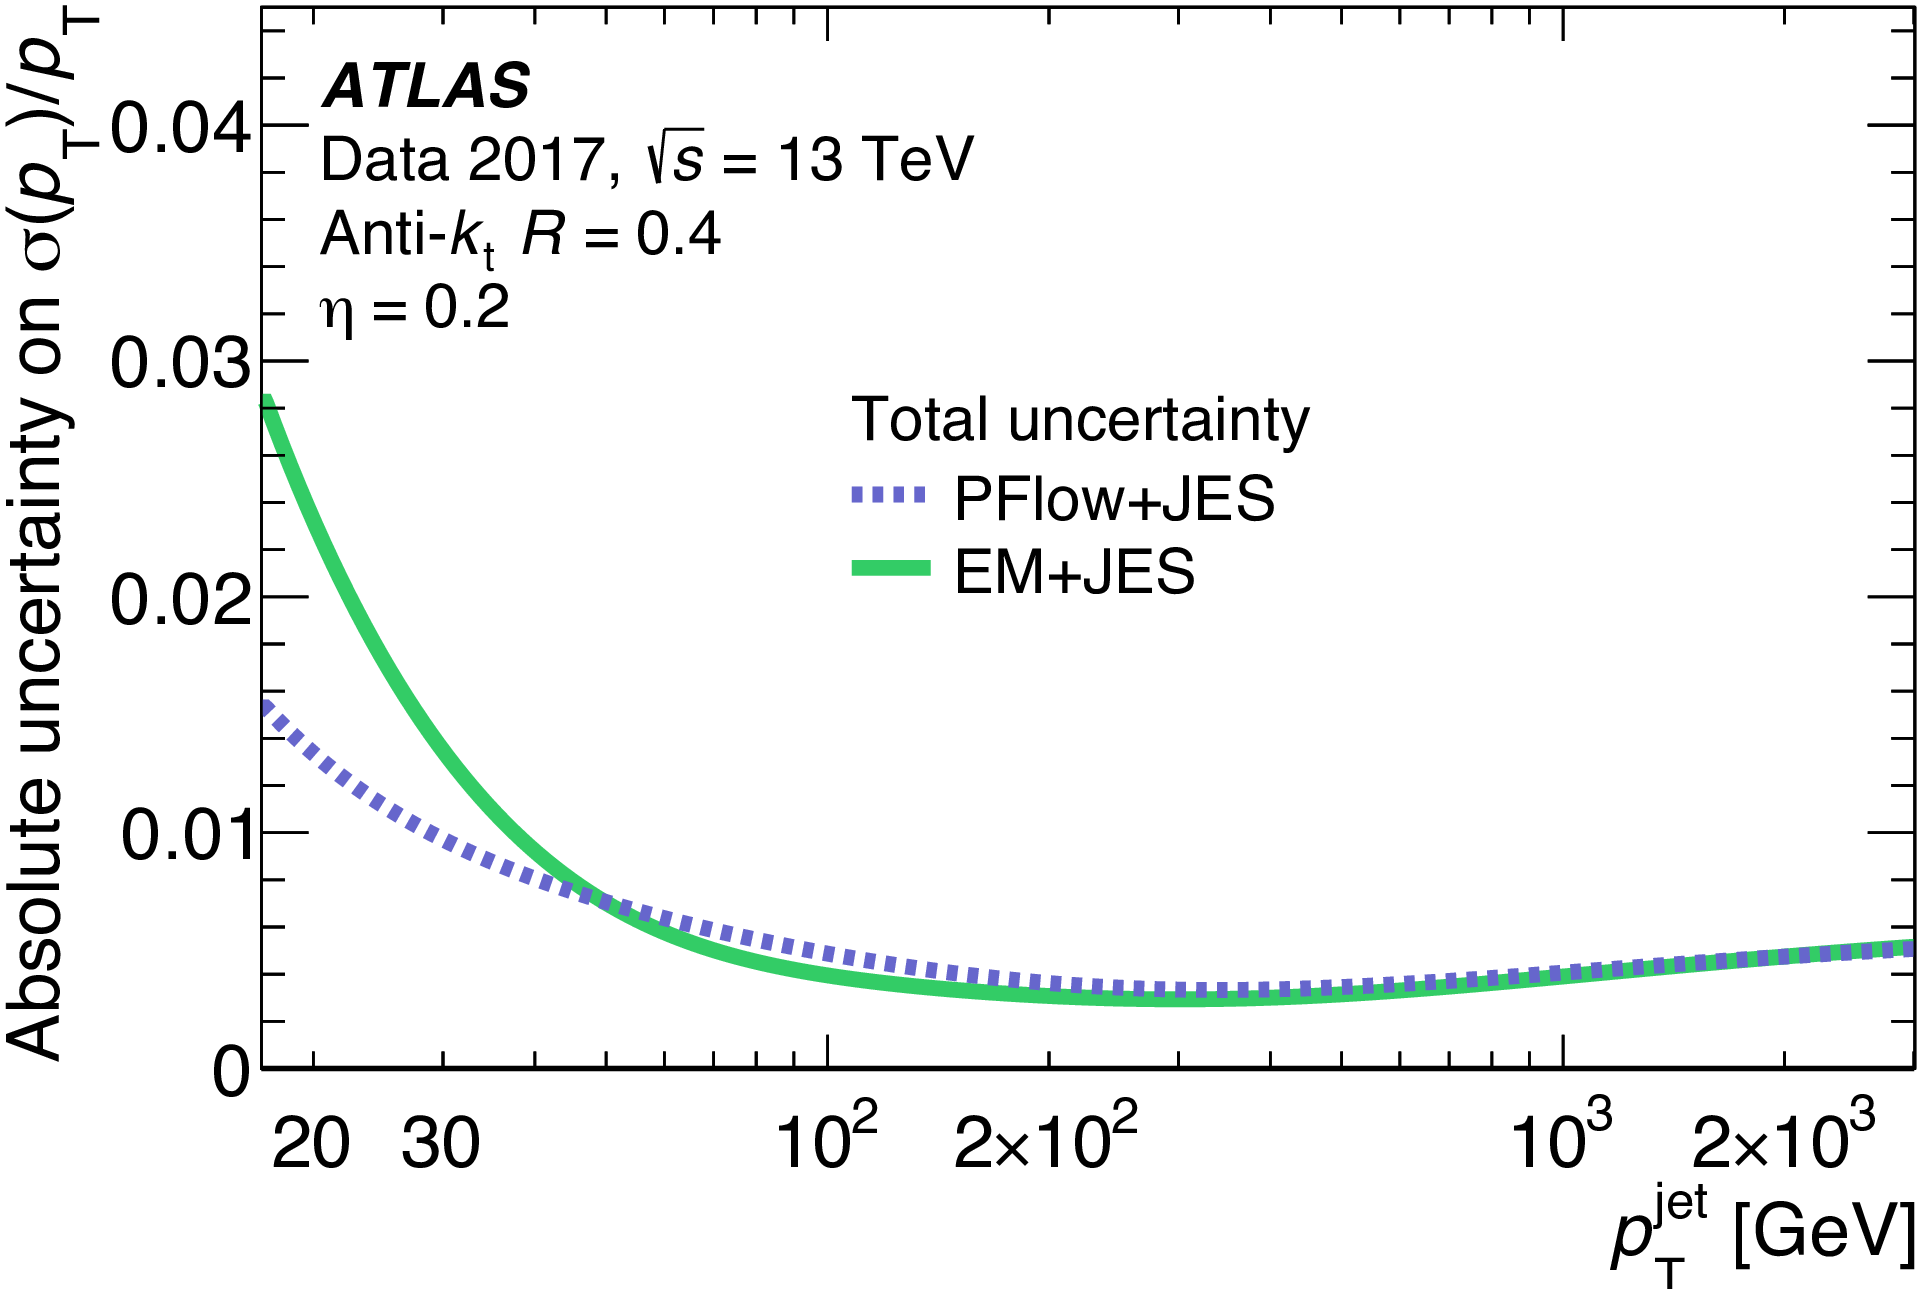
\includegraphics[width=\textwidth]{plots/atlas/JERa.png}
%    \caption{}
%    \label{fig:jer:a}
%\end{subfigure}
%\hfill
%\begin{subfigure}[b]{0.46\textwidth}
%    \centering
%    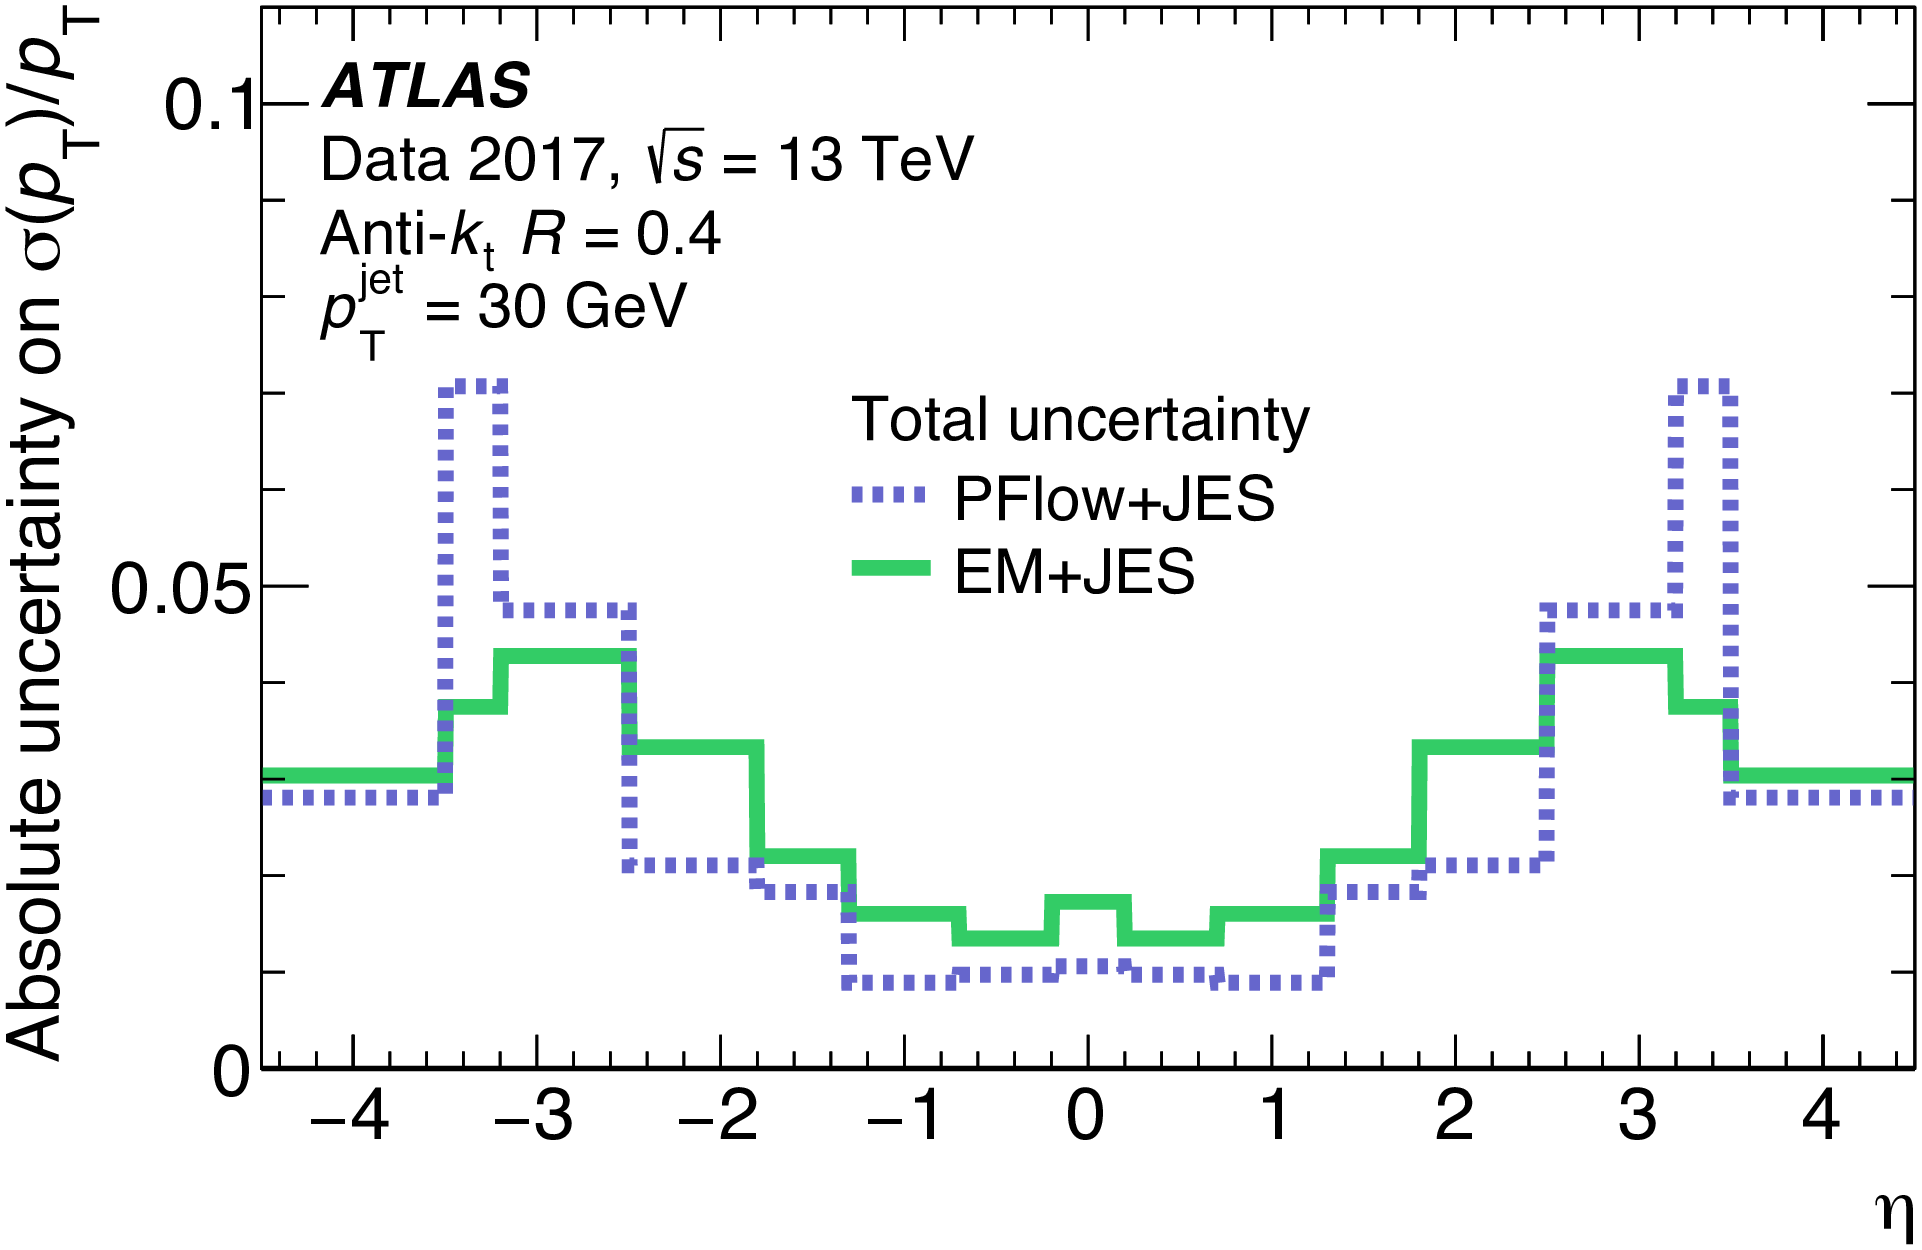
\includegraphics[width=\textwidth]{plots/atlas/JERb.png}
%    \caption{}
%    \label{fig:jer:b}
%\end{subfigure}
%\caption{Absolute uncertainty on the fractional JER for calibrated small-R PFlow and EMTopo jets for 2017 data. (a) shows the $\eta=0.2$ region with \pt. (b) shows the JER for 30\GeV jets with $\eta$. Figures from \cite{Atlas:smallrcali}.\label{fig:jer}}
%\end{figure}
%
\subsubsection{Jet Flavour Tagging}
Identifying jets containing $b$- and $c$-hadrons is very important in the context of precision electroweak measurements (for example \cite{Atlas:Hbb,Atlas:Hcc}). In the VBS measurement discussed in Chapter \ref{sec:vbswy}, $b$-tagging is of importance due to large backgrounds from top quarks, which decay to a $W$-boson and a $b$-quark. 

Because third generation quarks have a large CKM Suppression (little mixing between quark families), $b$-hadrons tend to have a large decay length. Furthermore, $b$-hadrons formed from the fragmentation of $b$-quarks tend to carry a large fraction of the intial quark momentum. This means that $b$-hadrons are likely to have a large Lorentz boost. The combination of these effects results in prominent displaced vertices. This detector signature is exploited in $b$-jet tagging algorithms, such as the \textit{DL1r} multivariate algorithm used for the $W\gamma$ VBS measurement \cite{Atlas:btagging}. When implementing $b$-tagging in an analysis, a tagging efficiency (the rate at which a true $b$-jet is identified correctly) working point needs to be selected depending on efficiency and purity requirements \cite{Buckley:PCP}. 

\subsubsection{Missing Tranverse Energy}

Since protons travelling along the LHC beamline carry no momentum component in the transverse plane, the \pt in any collision must be conserved. However, in many processes, an imbalance in momentum is expected due to the production of neutrinos which don't interact with the ATLAS detector, but can carry significant \pt. The missing transverse momentum \ptmiss is given by $\ptmiss\equiv(p^{\text{miss}}_x,p^{\text{miss}}_y)$ and quantifies the momentum balance in the transverse plane. The magnitude of the vector \ptmiss is referred to as the \textit{missing transverse energy} (MET), \met:
\begin{equation}\label{eq:etmiss_sum}
    \met = \sqrt{(p^{\text{miss}}_{\mathrm{x}})^2+(p^{\text{miss}}_{\mathrm{y}})^2}.
\end{equation}
The direction of the \ptmiss in the transverse plane is defined as
\begin{equation}
    \phi^{\text{miss}}=\text{atan2}(p_y^{\text{miss}},p_x^{\text{miss}}),
\end{equation}
where the atan2$(y,x)$ function is defined to return the argument of the complex number $x+iy$, and is used over the arctan function as it covers the interval $(-\pi,\pi]$, rather than the $[-\frac{\pi}{2},\frac{\pi}{2}]$ interval covered by the arctan function.

The components $p^{\text{miss}}_{x(y)}$ are given by the negative vector sum of \textit{hard objects} and \textit{soft signals} in the event:
\begin{equation}
    p^{\text{miss}}_{x(y)}=-\sum_{i\in\{\text{hard objects}\}}p_{x(y),i}-\sum_{j\in\{\text{soft signals}\}}p_{x(y),j}.
\end{equation} 
The \textit{hard objects} refer to electrons, photons, muons, $\tau$ leptons, and jets, with a set of kinematic and object reconstruction quality requirements. The \textit{soft signals} refers to all detector signals for the triggered event which do not contribute to the hard objects. They include non-collision backgrounds such as scattered soft particles from the UE as well as signals from objects which do not satisfy the hard object selection criteria. 

The mutual exclusivity of the detector signal requires a well defined sequence of contributions as well a way of rejecting signals where overlaps are present. The usual reconstruction sequence for the hard objects is electron reconstruction, followed by photons, hadronically decaying $\tau$s, muons, and finally jets. Each of these objects are fully calibrated before they enter the \ptmiss calclation, such that contributions to \ptmiss do not arise due to incorrect energy scales. All electrons passing some selection criteria are included in the \ptmiss reconstruction first, and particles further in the sequence are rejected if there is a shared calorimeter signal with an earlier particle in the sequence. 

The contributions from soft signal are calculated in the following way. Good quality tracks in \pt range of $400\MeV<\pt<100\GeV$ are selected. The tracks are then extrapolated to a high granularity region of the EM calorimeter, and a $\Delta R$ check is performed to assess whether the track is associated with an calorimeter deposits. Those tracks which do not have calorimeter deposits are retained in the soft term, and those which do match to a topo-cluster, are also retained, but the topo-cluster is removed in order to take advantage of the improved \pt resolution of the ID. For cases where multiple topo-clusters are matched to a given track, the highest energy cluster is retained. Any left over topo-clusters which have not been matched to tracks or discarded are also added to the soft term. The performance of \met and \ptmiss reconstruction is assessed using $Z\rightarrow ee/\mu\mu$ events, where selections of the dilepton invariant mass around the $Z$ invariant mass peak provide clean signal with no expected contributions for \met. Events involving leptonic $W$ decays in association with jets are used to study cases with true \MET \cite{Buckley:PCP,Atlas:met}. % The signals from muons are unique in that, in most cases, they are reconstructed solely from ID and MS contributions, as such the decision of where muons are reconstructed in this sequence is of little importance.
%The Missing Transverse Energy (MET), \met, is defined using the components $E_{\mathrm{x(y)}}^{\text{miss}}$ along the $x$ and $y$ axes: 
%\begin{equation}\label{eq:etmiss_xy}
%  E_{\mathrm{x(y)}}^{\text{miss}}=E_{\mathrm{x(y)}}^{\text{miss},e}+E_{\mathrm{x(y)}}^{\text{miss},\mu}+E_{\mathrm{x(y)}}^{\text{miss},\gamma}+E_{\mathrm{x(y)}}^{\text{miss,jets}}+E_{\mathrm{x(y)}}^{\text{miss,Soft-Term}},
%\end{equation}
%where each term is defined as the magnitude of the negative vector sum of the reconstructed objects passing the preselection cuts, projected on to the $x$ or $y$ axis. The "Soft-Term" component is calculated entirely from primary vertex tracks not matched to the physics objects associated with the other "Hard-Terms". This is the "Track Soft-Term", or TST. Since tracks can be matched to a primary vertex, the TST \met is relatively robust to pile-up contributions.

%The \met is calculated using calibrated physics objects, meaning corrections applied to the physics objects are taken into account in the \met calculation. The preselection cuts on the physics objects defining the hard terms are: $\pt^{\gamma}>12\GeV$, $\pt^{e(\mu)}>7\GeV$, and $\pt^{\text{jet}}>25\GeV$. The Tight working point is used in which forward jets are required to have $pT > 30$.%The baseline fiducial region has a cut on the MET of $\met > 30GeV$.

\subsubsection{Taus}
Tau leptons decay (decay length $87\mu\text{m}$) either leptonically or hadronically before reaching the active parts of the ATLAS detector. About 35\% of the time, taus decay to a tau neutrino, electron/muon, and lepton neutrino mediated via an off-shell $W$ boson. 65\% of the decay modes involve the tau decaying hadronically, where in 72\% and 22\% of the time one or three charged pions are produced, respectively. Additionally, 68\% of hadronic tau decays involve the production of a neutral pion. Leptonic tau decays cannot be distinguished from electrons or muons at the interaction point, however hadonic tau decays have a very specific signature. Firstly, the invariant mass of the system of jets must be less than the tau invariant mass of around 1.8\GeV, and the predictable production of charged pions result in either one or three tracks in the ID \cite{Atlas:trackmultiplicity}. Taus also have very collimated showers compared to QCD jets, this is because QCD jets are initiated by partons carrying colour charge, where the hadronisation process results in multiple quark and gluon emissions due to them being colour-connected to the initial parton. Additionally, tau tracks tend to have large impact parameters due to the significant decay length of the tau. Taus are reconstructed initially as jets using the anti-$k_t$ with $R=0.4$. Afterwards, a multivariate analysis uses various jet properties to tag the taus \cite{Buckley:PCP,Atlas:tau}. 
\begin{figure}[t]
   \centering
   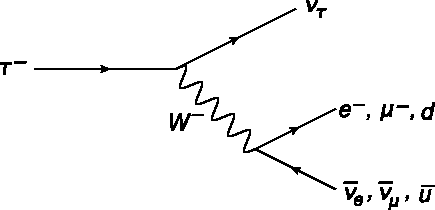
\includegraphics[width=0.5\textwidth]{plots/atlas/taudecay.pdf} 
   \caption{Feynman diagram for tau decays via off-shell $W$ boson. From \cite{Buckley:PCP}. \label{fig:taudecay}}
\end{figure}
\FloatBarrier
%------------------------------------------------------------------------- 

%-------------------------------------------------------------------------
\newpage
\chapter{In-situ Calibration of Large-R Jets Using Direct Balance in Z+Jet Events}
\label{sec:insitu}
\section{Introduction}
This chapter describes the methods used to derive the first Jet Energy Scale (JES) in-situ calibrations for large-R jets using \zjets events, for jets that have been reconstructed using UFO input objects (Section \ref{sec:atlas:jets}). The JES is derived in the region $|\eta|<0.8$, for large-R jets with $152.2\GeV < \pt < 754.6\GeV$ for \zee events and $156.9\GeV<\pt<745.4\GeV$ for the \zmm events. The calibration was derived using the ``InsituBalance'' framework, which is a software package originally created for the MultiJet-Balance calibration \cite{Atlas:largercali}, but was adapted by the author for the Z+jet in-situ calibrations.% The workflow of the InsituBalance framework is outline in Figure \ref{fig:insituworkflow}, which is a flowchart that shows each step of the calibration in going from the input samples to the final graphs which are passed on the insitu combination effort. 
%In the insitu combination, the results from all insitu calibration steps are combined to yield the final calibrations used by physics analyses.
%\begin{figure}[t]
%    \centering
%    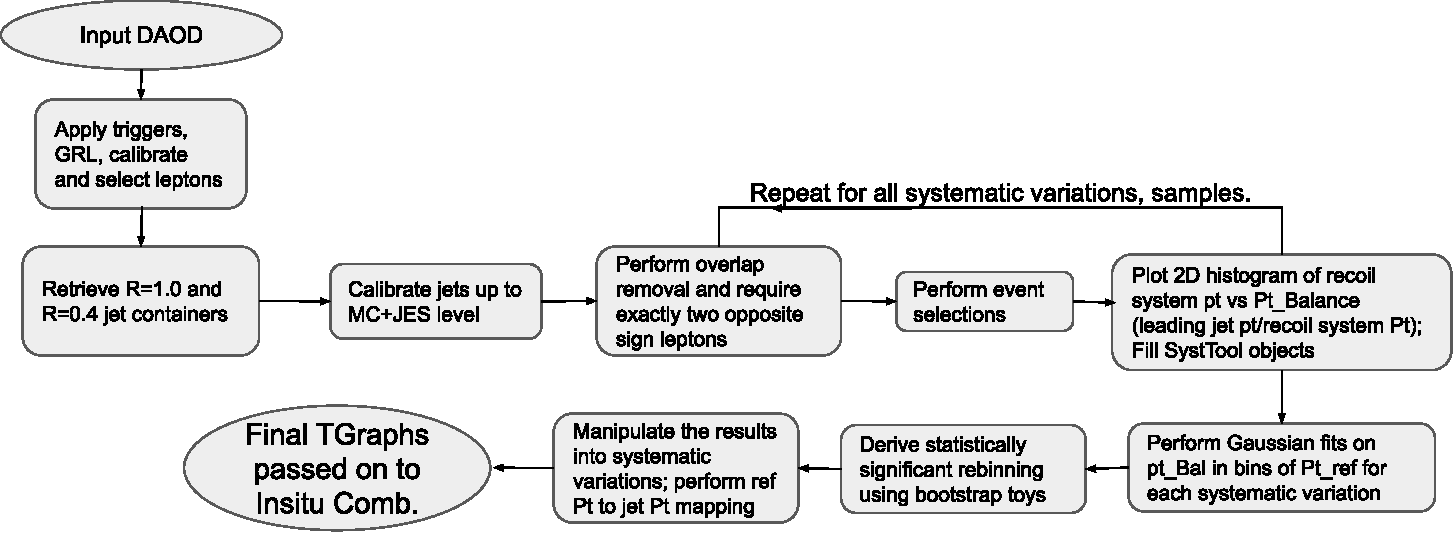
\includegraphics[width=\textwidth]{plots/insitu/workflow.pdf}
%    \caption{Flowchart showing the workflow for the InsituBalance framework used in the deriving the $Z+$jet large-R calibration.\label{fig:insituworkflow}}
%\end{figure}

\section{Jet Calibration\label{sec:jetcal}}

After reconstruction, jets are calibrated so that the average reconstructed jet \pt and mass, $m$, is restored to that of particle-level (also called \textit{truth}) jets. These are simulated jets which have not gone through detector simulation. The correction factors are known as jet energy/mass scale (JES,JMS) factors. The JES+JMS calibration consists of a series of steps outlined in Figure \ref{fig:jetcali}, where the steps are slightly different for small-R and large-R jets.

\begin{figure}[t]
    \centering
    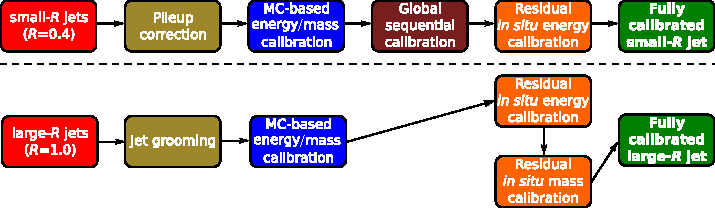
\includegraphics[width=\textwidth]{plots/atlas/calichain.pdf}
    \caption{Jet calibration chain for small-R and large-R jets. Adapted from \cite{Schramm:2017frb}.\label{fig:jetcali}}
\end{figure}

After anti-$k_t$ jet building of the detector-level (also called \textit{reco}) jets - these are simulated jets which have gone through detector simulation - a reference set of truth jets are reconstructed and geometrically matched to the reco jets using a $\Delta R$ matching requirement. Small-R jets then have a pileup correction applied in the first stage of the calibration chain. The purpose of this step is to correct for the contribution to the jet energy due to pileup. The correction consists of two steps: the jet area-based correction and the residual pileup correction. The area-based corrections subtracts the expected contribution from pileup based on the area of the jet and the median \pt density in the event. After this correction there is still a dependence of the difference between the reco jet and truth jet \pt on the pileup activity. A residual correction is therefore implemented, parametrised in the number of PVs ($N_{\text{PV}}$), and $\mu$ which quantify in-time and out-of-time pileup\footnote{In-time pileup refers to $pp$ collisions from the same bunch-crossing as the interaction of interest, whereas out-of-time pileup refers to $pp$ collisions occurring in bunch-crossings just before and after the interaction of interest.} respectively.

Large-R jets do not have a pileup correction applied in the same way as small-R jets. Since the jet volume of large-R jets encloses a larger fraction of the calorimeter than small-R jets, they are significantly more sensitive to pileup. In spite of the fact that large-R jets represent high \pt objects, and pileup is typically low \pt, the angular structure of large-R jets can be affected, limiting the jet substructure performance. For this reason, ``grooming'' algorithms are applied to large-R jets. Grooming algorithms remove jet constituents, and rebuild the jets from the remaining constituents. The ``trimming'' algorithm \cite{Insitu:trimming} was prevalent for large-R jets in early Run-2 analyses, where regions of the jet with small relative contributions to the jet \pt are removed. The latest recommendations use variations of the ``Soft-Drop'' algorithm \cite{Insitu:softdrop}, which is a technique for removing soft and wide-angle radiation from a jet. With the reconstruction of large-R truth jets, the same grooming algorithm is applied as the reco jets.  

In the next step of the calibration chain, the MC-based JES and JMS corrections are derived using dijet events. The \pt and mass responses are defined as $R_{\pt}=\langle\pt^{\text{reco}}/\pt^{\text{true}}\rangle$ and $R_{m}=\langle m^{\text{reco}}/m^{\text{true}}\rangle$, where the averages are determined from Gaussian fits (recently, small-R UFO jets were calibrated using a ``numerical inversion'' technique which uses piecewise polynomials called ``splines'' to fit the response \cite{Atlas:smallrufo}). For the JES calibration, the response fits are performed in bins of jet energy and detector pseudorapidity (pseudorapidity relative to the geometrical center of the ATLAS detector, rather than the hard scatter PV). The JES factor, $c_{\text{JES}}=1/R_{\pt}$ is then smoothed in energy and $\eta_{\text{det}}$. A correction to $\eta$, $\Delta\eta$ is also derived. After $c_{\text{JES}}$ is calculated, a correction to the jet invariant mass is derived\footnote{Corrections to the large-R jet mass in particular are important since the mass is more sensitive than the \pt to soft, wide-angle contributions, calorimeter geometry and topo-cluster merging and splitting. Moreover, the large-R jet mass is a powerful substructure variable used for discriminating between QCD jets and hadronically decaying massive particles.}. Jet mass corrections are derived using the same procedure as the JES, and in bins of $E_{\text{reco}}$, $\eta^\text{det}$, as well as $\log(m_{\text{reco}}/E_{\text{reco}})$. The JMS calibration factor ($c_{\text{JMS}}=1/R_m$) is applied only to the mass of the jet while keeping the energy fixed, and allowing the \pt to vary.  The $\phi$  coordinate is not affected by the calibration. The calibrated kinematic variables are thus given by: 
\begin{equation}
    E_{\text{reco}}=c_{\text{JES}}E_0,\hspace{5pt}m_{\text{reco}}=c_{\text{JES}}c_{\text{JMS}}m_0,\hspace{5pt}\eta_{\text{reco}}=\eta_0+\Delta\eta,\hspace{5pt}\pt^{\text{reco}}=c_{\text{JES}}\frac{\sqrt{E_0^2-c_{\text{JMS}}^2m_0^2}}{\cosh(\eta_0+\Delta\eta)},
\end{equation}
where the quantities with a 0 subscript refer to those prior to any calibration, but after jet grooming (for the large-R case) \cite{Atlas:largercali,Atlas:Schramm}.

For small-R jets, there is an additional step after the MC-based calibration, which is the Global Sequential Calibration (CSC). This step aims to improve the relative \pt resolution given by $\frac{\pt^{\text{JES+JMS}}/\pt^{\text{true}}}{\langle\pt^{\text{JES+JMS}}/\pt^{\text{true}}\rangle}$, where $\pt^{\text{JES+JMS}}$ is the jet transverse momentum after the MC-based calibration. The GSC also corrects for differences in the \pt response for gluon initiated and quark initiated jets. This correction is derived based on global jet observables such as the longitudinal shower structure, and tracking information, and takes the form of a sequence a multiplicative corrections. Recently a neural network approach (Global Neural Network Calibration) has been explored which is an alternative to this sequential correction and allows for correlated global observables to be used in deriving the calibration \cite{Atlas:smallrnewtechniques}.

The final calibration stage is the \textit{in-situ} calibration. Differences in the jet response can arise between data and simulation due to imperfect detector modelling, pileup, particle-detector interactions, the UE, and jet formation. The in-situ correction factor is defined as the double ratio of the response in data divided by the response in MC:
\begin{equation}
    c=\frac{\mathcal{R}^{\text{data}}_{\text{in-situ}}}{\mathcal{R}^{\text{MC}}_{\text{in-situ}}},
\end{equation}
where the response is defined as:
\begin{equation}
    \mathcal{R}_{\text{in-situ}} = \Bigg\langle\frac{\pt^{\text{jet}}}{\pt^{\text{ref}}}\Bigg\rangle,
\end{equation}
and $\pt^{\text{ref}}$ is defined as the \pt of a well-measured reference object, and $\pt^{\text{jet}}$ is the transverse momentum of the jet being calibrated. $\mathcal{R}_{\text{in-situ}}$ is transformed from a function of $\pt^{\text{ref}}$ to a function of jet transverse momentum through a process of numerical inversion (see Section \ref{sec:insitu}) prior to the double ratio $c$ calculation. The response $\mathcal{R}_{\text{in-situ}}$ is sensitive to secondary effects such as out-of-cone radiation, where jets from QCD radiation are not captured by the jet cone. The expectation is therefore that $\mathcal{R}_{\text{in-situ}}$ is skewed below 1, and these effects are partially mitigated through the event selection. The double ratio $c$, however, is robust to such effects, so long as they are not mismodelled in simulation. 

There are three stages of the in-situ calibration which are performed sequentially. First, the inter-$\eta$ calibration uses dijet events to correct the energy scale of forward jets ($0.8 < |\eta_{\text{det}}| < 4.5$) to that of central jets ($|\eta_{\text{det}}|<0.8$). The reason for deriving this correction is that the in-situ calibrations that follow are derived solely in the central region as forward jets have increased response variations due to the more complicated detector structure in the forward regions. The $\eta$-inter calibration requires two back-to-back jets in the transverse plane from different $\eta_{\text{det}}$ regions. All in-situ calibration steps exploit the momentum balance of the system. In the case of the $\eta$-inter calibration, the two jets are required to have equal and opposite \pt to satisfy the momentum balance. A quantity called the momentum asymmetry is constructed, which is the difference of the jet transverse momenta divided by the average jet \pt, and quantifies the response difference between the two detector regions. For a given pair of $\eta_{\text{det}}$, the asymmetry can be used to define the calibration factors.

The next step of the calibration chain exploits the \pt balance in $\gamma/Z(\rightarrow ee/\mu\mu)$+jet events. Electrons and photons are accurately calibrated as described in Section \ref{sec:egamma}, and the muons are calibrated using $Z\rightarrow\mu\mu$, $J/\Psi\rightarrow\mu\mu$ and $\Upsilon\rightarrow\mu\mu$ events. These methods benefit from the accurate knowledge of the energy scale and resolution of leptons and photons. These in-situ calibrations are called the direct-balance (DB) calibrations. The DB response is:
\begin{equation}
    \mathcal{R}_{\text{DB}}=\langle\frac{\pt^{\text{j1}}}{\pt^{\text{ref}}}\rangle,\hspace{5pt}\pt^{\text{ref}}=\pt^{Z\gamma}|\cos(\Delta\phi)|,
\end{equation}
where $\pt^{\text{j1}}$ is the \pt of the leading jet, and $\Delta\phi$ is the azimuthal separation between the photon or the reconstructed $Z$. The reason for the $|\cos\Delta\phi|$ factor is to reduce the effect of ``out-of-cone'' (OOC) radiation, which is additional QCD radiation from the jet which is not captured in the jet cone during jet building. The reference object is colour neutral, hence there is more QCD radiation in the jet hemisphere resulting in a bias which takes the response below unity. This $|\cos\Delta\phi|$ factor reduces the effect of this bias by balancing the momentum of the reference object onto the jet axis in the transverse plane. 

Events are selected by requiring low \pt jet veto, and a minimum requirement on the $\Delta\phi$ between the leading jet and the reference system. Independent calibration factors are derived for $Z(\rightarrow ee)$+jet, $Z(\rightarrow \mu\mu)$+jet and $Z\gamma$+jet DB. The $Z$+jet calibration is limited to the statistically significant \pt range of $Z$ boson production, and is therefore only relevant at low and medium \pt in the range of around $17 < \pt < 800\GeV$. The complementary $\gamma$+jet measurements which are limited by small numbers of events at high \pt and by dijet contamination, are relevant at around $30<\pt<2000\GeV$ with a limited precision at $\pt<100\GeV$.

For the calibration of small-R jets, an additional in-situ calibration called the Missing Momentum Fraction (MPF) method is also used to complement the DB calibrations. The MPF method measures the \pt balance between the reference object and the full hadronic recoil (i.e. including any QCD OOC radiation). This method is very robust against pileup and the UE, and covers a similar kinematic range to $\gamma$+jet DB. In the final stage of the in-situ calibration, a \pt balance method using multijet events is implemented to extend the kinematic range of the calibration to larger transverse momenta than what could be achieved by $\gamma$+jet. Recent developments in the in-situ calibration have allowed for a precision of the correction factor at level of $1\%$. Additionally, recent developments have allowed for measurements of the JES for b-tagged jets at the level of $1\%$ using $\gamma$+jet direct balance. These measurements have the potential to improve the precision of analyses which are very sensitive to the b-jet JES such as $H\rightarrow b\bar{b}$ and top mass measurements \cite{Atlas:smallrnewtechniques,Atlas:largercali,Atlas:smallrcali}.

For the case of large-R jets, an in-situ calibration for the JMS is also calculated. Two independent methods are used to derive these corrections. The $R_{\text{trk}}$ method uses calorimeter-to-tracker response ratios. This method was used for calibrating large-R LCTopo jets for Run-2 analyses, where the fact that tracker and calorimeter provide independent measurements is exploited in order to validate the modelling of large-R jet properties. The forward folding method uses a high purity, high \pt large-R jet sample from $t\bar{t}$ events, where one of the top quark decays hadronically ($t\rightarrow b+W(\rightarrow\text{jets})$), and the other decays via a leptonically decaying W ($t\rightarrow b+W(\rightarrow l\nu)$). The response is obtained from fits to the top and W mass peaks in the invariant mass distribution of the large-R jet of the hadronically decaying top candidate. The W mass peak is present when a large-R b-jet veto is applied, and the top mass peak is present when the large-R jet is b-tagged. Two independent methods for calculating the large-R jet mass are implemented. These are the calorimeter jet mass, $m^{\text{calo}}$, and the track-assisted jet mass ($m^{\text{TA}}$). For a large-R calorimeter jet $J$ with topo-cluster constituents $i$ with energy $E_i$ and momentum $\mathbf{p}_i$, the calorimeter-based jet mass is defined as:
\begin{equation}
    m^{\text{calo}}=\sqrt{(\sum_{i\in J}E_i)^2-(\sum_{i\in J}\mathbf{p}_i)^2},
\end{equation}
and the track-assisted jet mass is defined as:
\begin{equation}
    m^{\text{TA}}=\frac{\pt^\text{calo}}{\pt^\text{track}}\times m^{\text{track}},
\end{equation}
where the track invariant mass, $m_{\text{trk}}$, is assumed to be the pion mass. The values for the response in data and MC are extracted simultaneously in a fit known as \textit{forward folding} \cite{Atlas:largercali}.

%\clearpage
\section{Data and MC samples\label{sec:insitu:dataandmcsamples}}
 Proton-proton collision data at a centre-of-mass energy of $\sqrt{s}=13\TeV$ are using in the in-situ calibration. The data are required to pass unprescaled dielectron or dimuon triggers depending on whether the $Z$-boson decays to electrons or muons, respectively. These triggers are shown in Table \ref{tab:Insitu:trigger}, and depend on the year the data were recorded.
\begin{table}[t]
\centering
\begin{tabular}{|c||c|c|c|}
\hline
& \textbf{Year} & \textbf{Level1} & \textbf{HLT} \\ \hline \hline
\multirow{7}{*}{\textbf{Dielectron trigger}} 
%& \multirow{2}{*}{2015} & xyz \\ && centred on $\et=12\GeV$ & \multirow{2}{*}{N/A} \\
& \multirow{2}{*}{2015} & $\et>10\GeV$(*); & $\et>12\GeV$; \\ & & Hadronic activity veto & loose ID \\ \cline{2-4} & \multirow{2}{*}{2016} & $\et>13\GeV$(*); & $\et>15\GeV$; \\ & & Hadronic activity veto & vloose ID, $d0$ unused \\ \cline{2-4} & \multirow{3}{*}{2017/2018} & $\et>15\GeV$(*); & \multirow{2}{*}{$\et>17\GeV$;} \\ & & Hadronic activity veto; & \multirow{2}{*}{vloose ID, $d0$ unused} \\ & & Isolated & \\
\hline \hline
\multirow{4}{*}{\textbf{Dimuon trigger}} 
%& \multirow{2}{*}{2015} & xyz \\ && centred on $\et=12\GeV$ & \multirow{2}{*}{N/A} \\
& \multirow{2}{*}{2015} & \multirow{2}{*}{$\et>10\GeV$} & \multirow{2}{*}{ $\et>10\GeV$} \\ &&&\\ \cline{2-4} & \multirow{2}{*}{2016/2017/2018} & \multirow{2}{*}{$\et>10\GeV$} & \multirow{2}{*}{$\et>14\GeV$} \\ & & & \\
\hline
\end{tabular}
\caption{An $\eta$-dependence of the L1 trigger threshold is denoted by (*).\label{tab:Insitu:trigger}}
\end{table}    
 The dataset corresponds to an integrated luminosity of 139\invfb \cite{LUMI}. The data are required to pass data-quality criteria to ensure the data were taken during periods where the detector subsystems were fully functioning. This is achieved via ``GoodRunsLists (GRLs)'', which are provided by the ATLAS Data Quality group.

The nominal sample of \zjet events is generated using \POWHEGBOX v1 \cite{Insitu:powheg1,Insitu:powheg2,Insitu:powheg3}, with NLO matrix-element (ME) accuracy in perturbative QCD for inclusive $Z$ production. The CT10 PDF set is used in the ME calculation \cite{Insitu:ct10}. The parton-level final state is interfaced with \PYTHIA (v8.186) \cite{Insitu:pythia} for generating the parton shower (PS), hadronisation, and multi parton interactions (MPI), utilising the \AZNLO tuned parameter set \cite{Insitu:aznlo}. The \PHOTOSpp program \cite{Insitu:photos} is used for the modelling of QED emissions from electroweak vertices and charged leptons. EvtGen 1.2.0 \cite{Insitu:evtgen} is used for the properties of $b$- and $c$-hadron decays.

For evaluating the systematic uncertainty due to MC generator choice, a second \zjets sample is generated using \SHERPA{2.2.1} \cite{Insitu:sherpa,Insitu:sherpa22} and is subdivided (sliced) into discrete regions of $\text{max}(H_\text{T},p_{\text{T}}^V)$, with boundaries at [0,70,140,280,500,1000,6500]\GeV, where $H_\text{T}$ is defined as the scalar sum of all partonic jet transverse momenta, and $p_{\text{T}}^V$ is the mass of the dilepton system. NLO-accurate matrix elements for up to two jets, and LO-accurate matrix elements for up to 4 jets are calculated with \COMIX \cite{Insitu:comix}. The $b$- and $c$-quarks are treated as massless at the ME calculation, and massive in the parton shower. The parton showering is conducted by \CSShower \cite{Insitu:csshower}, which is based on Catani-Seymour dipole factorisation \cite{Insitu:csalgorithm}. Virtual QCD corrections to the ME are derived with \OPENLOOPS \cite{Insitu:openloops}. The NLO matrix elements for any given jet multiplicity is matched to parton shower, and different jet multiplicities are then merged according to the CKKW matching procedure \cite{Insitu:ckkw1,Insitu:ckkw2} and extended to NLO accuracy using the \MEPSatNLO prescription \cite{Insitu:meps}. The \NNPDF PDF set \cite{Insitu:nnpdf} is used with dedicated parton shower tuning developed by the \SHERPA authors. The invariant mass of the dilepton system is required to be at least $40\GeV$ \cite{Insitu:zjetmc}. The MC event simulations are interfaced with the \GEANT toolkit \cite{GEANT4} for detailed modelling of the ATLAS detector response \cite{Insitu:atlassim}. %These simulations are compared to a data set of $pp$ collisions delivered by the LHC at a centre-of-mass energy of $\sqrt{s}=13\TeV$ during the 2015-2018 period. The data are required to pass unprescaled dielectron or dimuon triggers depending on whether the \zeejet or \zmmjet calibration is performed. These triggers are shown in Table \ref{tab:Insitu:trigger}.
%\begin{table}[ht]
%\centering
%\begin{tabular}{|c||c|c|c|}
%\hline
%& \textbf{Year} & \textbf{Level1} & \textbf{HLT} \\ \hline \hline
%\multirow{7}{*}{\textbf{Dielectron trigger}} 
%& \multirow{2}{*}{2015} & xyz \\ && centred on $\et=12\GeV$ & \multirow{2}{*}{N/A} \\
%& \multirow{2}{*}{2015} & $\et>10\GeV$(*); & $\et>12\GeV$; \\ & & Hadronic activity veto & loose ID \\ \cline{2-4} & \multirow{2}{*}{2016} & $\et>13\GeV$(*); & $\et>15\GeV$; \\ & & Hadronic activity veto & vloose ID, $d0$ unused \\ \cline{2-4} & \multirow{3}{*}{2017/2018} & $\et>15\GeV$(*); & \multirow{2}{*}{$\et>17\GeV$;} \\ & & Hadronic activity veto; & \multirow{2}{*}{vloose ID, $d0$ unused} \\ & & Isolated & \\
%\hline \hline
%\multirow{4}{*}{\textbf{Dimuon trigger}} 
%& \multirow{2}{*}{2015} & xyz \\ && centred on $\et=12\GeV$ & \multirow{2}{*}{N/A} \\
%& \multirow{2}{*}{2015} & \multirow{2}{*}{$\et>10\GeV$} & \multirow{2}{*}{ $\et>10\GeV$} \\ &&&\\ \cline{2-4} & \multirow{2}{*}{2016/2017/2018} & \multirow{2}{*}{$\et>10\GeV$} & \multirow{2}{*}{$\et>14\GeV$} \\ & & & \\
%\hline
%\end{tabular}
%\caption{An $\eta$-dependence of the L1 trigger threshold is denoted by (*).\label{tab:Insitu:trigger}}
%\end{table}    
%The dataset corresponds to an integrated luminosity of 139 \invfb \cite{LUMI}. The data are required to pass data-quality criteria. This is to ensure that the data taken during periods where the detector subsystems were not fully functioning; where there where large amount of detector noise; or where there were read-out issues are discarded. This is achieved via GoodRunsLists (GRLs):
%\begin{itemize}
%    \item 
%    \begin{verbatim} GoodRunsLists/data15_13TeV/20170619/data15_13TeV.periodAllYear_DetStatus-v89-pro21-02_Unknown_PHYS_StandardGRL_All_Good_25ns.xml
%    \end{verbatim}
%    \item 
%    \begin{verbatim} GoodRunsLists/data16_13TeV/20180129/data16_13TeV.periodAllYear_DetStatus-v89-pro21-01_DQDefects-00-02-04_PHYS_StandardGRL_All_Good_25ns.xml 
%    \end{verbatim}
%    \item 
%    \begin{verbatim} GoodRunsLists/data17_13TeV/20180619/data17_13TeV.periodAllYear_DetStatus-v99-pro22-01_Unknown_PHYS_StandardGRL_All_Good_25ns_Triggerno17e33prim.xml
%    \end{verbatim}
%    \item 
%    \begin{verbatim} GoodRunsLists/data18_13TeV/20190318/data18_13TeV.periodAllYear_DetStatus-v102-pro22-04_Unknown_PHYS_StandardGRL_All_Good_25ns_Triggerno17e33prim.xml
%    \end{verbatim}
%\end{itemize}
%
%\begin{VerbItem}
%    GoodRunsLists/data15_13TeV/20170619/data15_13TeV.periodAllYear_DetStatus -v89-pro21-02_Unknown_PHYS_StandardGRL_All_Good_25ns.xml
%    GoodRunsLists/data16_13TeV/20180129/data16_13TeV.periodAllYear_DetStatus -v89-pro21-01_DQDefects-00-02-04_PHYS_StandardGRL_All_Good_25ns.xml 
%    GoodRunsLists/data17_13TeV/20180619/data17_13TeV.periodAllYear_DetStatus -v99-pro22-01_Unknown_PHYS_StandardGRL_All_Good_25ns_Triggerno17e33prim.xml
%    GoodRunsLists/data18_13TeV/20190318/data18_13TeV.periodAllYear_DetStatus -v102-pro22-04_Unknown_PHYS_StandardGRL_All_Good_25ns_Triggerno17e33prim.xml
%\end{VerbItem}
%
%JETM3 DAOD datasets are used which are designed specifically for the \zjets insitu calibration as well determination of the combined performance MET systematics. These derivations contain the relevant jets described in Section \ref{sec:jetdef}, and are skimmed by requiring two single or dilepton triggers, and two leptons with $\pt>\sim20\GeV$. 
%TODO: Write about derivations before the reconstruction section.
% Derived xAODs (DAODs) in the JETM3 format are used 
%
%Trigger requirements, ATLAS standard quality criteria, data from periods where detector subsystems not fully functional is discarded, or where there is large detector noise, or read-out problems - good run lists. Int lumi of 139\invfb.  of ATLAS detector data collected during run2 in the 2015-2018 data-taking period at a centre-of-mass energy of $\sqrt{s}=13\TeV$.
%\clearpage
\section{Jet definitions \label{sec:jetdef}}
The large-R jets, which are the subject of the in-situ calibration described in this chapter, are built from UFO jet input objects \cite{Atlas:UFO} using the anti-$k_t$ algorithm \cite{Insitu:antikt} with radius parameter $R=1.0$. Constituent-level pile-up mitigation is applied using the Constituent Subtraction (CS) \cite{Insitu:cs} and SoftKiller (CS) \cite{Insitu:sk} algorithms. To remove soft contributions from the reconstructed jet, the Soft-Drop (SD) grooming algorithm \cite{Insitu:softdrop} is implemented. Additionally, fully calibrated small-R jets \cite{Atlas:PFlow2,Insitu:smallrcali} are used for \pt balancing and jet veto purposes. These jets are built from Particle Flow (PFlow) \cite{Atlas:PFlow} input objects using the anti-$k_t$ algorithm with radius parameter $R=0.4$. An overview of the definitions of the different jet objects is shown in Table \ref{tab:jetdefs}. The specific implementation of the jet clustering algorithm is taken from the \FASTJET package \cite{Insitu:fastjet1,Insitu:fastjet2}.

Large-R jets are calibrated in both data and simulation up the MC-based JES and JMS (MC JES+JMS) calibration scale \cite{Atlas:largercali}. Small-R jets are fully calibrated in both data and simulation, as described in Section \ref{sec:jetcal}.
%TODO: Describe smearing and describe CS+SK and Soft drop...
\begin{table}[t]
    \centering
    \begin{tabular}{|c||c|c|c|}
    \hline
    & \textbf{Algorithm} & $R$ & \textbf{Settings} \\ \hline \hline
    \multirow{4}{*}{\textbf{Jet input objects}} 
    & \multirow{2}{*}{Particle-Flow}          & \multirow{2}{*}{0.4} & \multirow{2}{*}{N/A} \\
                & & &        \\ \cline{2-4}
    & \multirow{2}{*}{Unified Flow Objects}    & \multirow{2}{*}{1.0} & \multirow{2}{*}{N/A} \\
                            & & &        \\
    \hline \hline
    \multirow{5}{*}{\textbf{Pile-up mitigation algorithms}} & \multirow{3}{*}{Constituent Subtraction} & \multirow{3}{*}{1.0}
                             & $A_g = 0.01$ \\
    &                        & & $\DeltaR_\text{max} = 0.25$ \\
    &                        & & $\alpha = 0$ \\ \cline{2-4}
    & \multirow{2}{*}{SoftKiller}             & \multirow{2}{*}{1.0}
                             & \multirow{2}{*}{$\ell = 0.6$} \\ &&& \\ 
    \hline \hline
    \multirow{2}{*}{\textbf{Jet grooming algorithms}}
    & \multirow{2}{*}{Soft-Drop} & \multirow{2}{*}{1.0}
                             & $\zcut$ = 0.1     \\
    &                      & & $\beta$ = 1    \\ \cline{2-4}
    \hline %inserts single line
    \end{tabular}
    \caption{Summary of the jet input object algorithms used for small-R ($R=0.4$) and large-R ($R=1.0$) jets, in addition to the specific pile-up mitigation and grooming algorithms used for the large-R jets. Since different versions of the pile-up and grooming algorithms exist, the exact parameters used relevant to these algorithms is shown in the last column. See \cite{Insitu:cs,Insitu:sk,Insitu:softdrop} for further details on the parameters.\label{tab:jetdefs}.} %Summary of pile-up mitigation algorithms, jet inputs, and grooming algorithms, the relevant parameters for each algorithm. \label{tab:jetdefs}}
    \end{table}    

%\clearpage
\section{Object Selections\label{sec:insitu:largerobj}}
\subsection{Electrons}
Electrons are reconstructed from ID tracks and calorimeter information as described in section \ref{sec:egamma}. Electrons are calibrated using the ``EgammaCalibrationAndSmearingTool'' with the ESModel ``es2018\tu R21\tu v0'' configuration using the decorrelation model setting ``1NP\tu v1'', which results in one non-zero scale and resolution systematic variation. Electrons are required to satisfy \textit{Loose} ID, and \textit{FCLoose} isolation requirements\footnote{``FC'' refers to ``FixedCut'', i.e. that a cut is put on the isolation variables themselves, rather than using cut maps to achieve a target selection efficiency.}, and are reconstructed within $|\eta|<2.47$, excluding the gap between the barrel and endcap EM calorimeters (1.36 < $|\eta|<1.52$). Electrons are required to satisfy $\pt>20\GeV$. Electrons are constrained to originate from the primary hard-scatter vertex through the requirements $|d_0|/|{\sigma_{d_0}}|<5$ and $|z_0\sin\theta|<0.5\mm$, where the impact parameters are defined in Section \ref{sec:tracking}.
\subsection{Muons}
Muons are reconstructed from MS tracks matched to ID tracks as described in Section \ref{sec:muon}. Muons are calibrated using the ``MuonCalibrationAndSmearingTool'' and the ``correctData\tu ID\\MS'' scheme which gives muon track resolution and momentum scale systematic variations on the seperate ID and MS components of the combined (CB) muon.  Muons are required to satisfy \textit{Loose} ID, and \textit{FCLoose} isolation requirements, and must be reconstructed within $|\eta|<2.4$ with $\pt>20\GeV$. Muons are constrained to originate from the primary hard-scatter vertex through the requirements $|d_0|/|{\sigma_{d_0}}|<3$ and $|z_0\sin\theta|<0.5\mm$, where the impact parameters are defined in Section \ref{sec:tracking}. The $\eta$ cut, ID quality, and track selections are performed by the ``MuonSelectionTool'', which also facilitaties vetoing events containing mis-reconstructed muons, as these objects tend to have significantly worse momentum resolution. Muons consistent with cosmic ray backgrounds are removed.
\subsection{Jets}
As described in Section \ref{sec:jetcal}, the \zjets in-situ calibration is designed to provide residual corrections to jets measured in the central detector region. Therefore, large-R jets are selected to be in the region $|\eta|<0.8$ and with $\pt>100\GeV$. Small-R jets are selected with $\pt>10\GeV$ and $|\eta|<4.5$ and are required to be $\Delta R>1.4$ from the leading large-R jet, to ensure no overlap. Small-R jets with $\pt<60\GeV$ and $|\eta|<2.4$ are required to satisfy the \textit{Tight} Jet Vertex Tagger (JVT) \cite{Insitu:JVT} working point in order to reject additional jets originating from pileup. The \textit{Medium} JVT working point is used as a systematic variation to assess the impact of the JVT selection on the calibration. % Small-R jets used to veto events with large QCD radiation are required to be separated from the the large-R jet where the response is being measured (J1).  
% TODO: Describe JVT
% TODO: Update isolation variables table to be consistent with the twiki page here: https://twiki.cern.ch/twiki/bin/view/AtlasProtected/IsolationSelectionTool#Leptons 
% FixedCutLoose 	electrons 	Cut: topoetcone20/pT < 0.2 	Cut: ptvarcone20/pT < 0.15 

%  1NP_v1: very simplified model. This is suggested for analyses which are not sensitive to the energy scale or resolution and that do not use categories in eta. All the physical effects are summed in quadrature and considered fully correlated in eta. Usually this approach give pessimistic (larger) systematics. Using this scheme it should be checked that in the fit the NPs relative to the calibration systematics are neither pulled nor over-constrained. If this happens it could mean that the analysis is sensitive to the calibration and its decorrelation and so a more detailed model is needed. FROM: https://twiki.cern.ch/twiki/bin/view/AtlasProtected/ElectronPhotonFourMomentumCorrection#Recommendation_for_run_2_data_in
\subsection{Overlap Removal}\label{sec:insitu:or}
To prevent detector signals from one object being used in the reconstruction of a different object, an object overlap removal procedure is applied according to the ATLAS standard overlap removal tool \cite{ORTool} in the following order:
\begin{itemize}
    \item If two electrons share the same track in the ID, the electron with the lowest \pt is rejected.
    \item Calorimeter muons are rejected against electrons if they share the same track in the ID.
    \item Electrons are rejected against muons if they share the same track in the ID.
    \item Small-R jets are rejected against electrons if $\Delta R<0.2$.
    \item Electrons are rejected against small-R jets if $\Delta R<0.4$.
    \item Small-R jets are rejected against muons if there are $<3$ tracks and either the jet and the muon are ghost-associated\footnote{With ``ghost-association'' particles can be associated to jets by treated them as particles with negligible \pt and clustering them within the jet \cite{Insitu:ghostassociation}.} or $\Delta R<0.2$. 
    \item Muons are rejected against small-R jets if $\Delta R<0.4$.
    \item Large-R jets are rejected against electrons if $\Delta R < 1.0$.
\end{itemize}

%\clearpage
\section{Event Selection}
Event selection criteria are applied such that the analysis is performed in a region that is populated by event topologies in which the reconstructed $Z$-boson's momentum is balanced by the momentum of the large-R jet (a so-called 2$\rightarrow$2 topology). Furthermore, to ensure the leptons are consistent with a Z-boson decay, lepton pairs are required to have the same flavour and opposite charge. The invariant mass of the dilepton system is required to be consistent with the invariant mass of the Z-boson, i.e. $66\GeV<m_{ll}<116\GeV$. The $2\rightarrow2$ topology selection is enforced by a veto on events in which (i) there is a small-R jet that carries a significant amount of the total jet momentum, and (ii) the large-R jet and the dilepton system are separated by $\Delta\phi(Z,J_1)\approx\pi$. The event selections and their variations for evaluating systematic uncertainties are listed in Table \ref{tab:evsel_insitu}. 

\begin{table}[t]
    \centering
    \resizebox{\textwidth}{!}{%
    \begin{tabular}{lccc}
        \hline
        Variable & Nominal Selection & Up Variation & Down Variation \\ \hline
        $\pt^{\mathrm{j_1}} $ & $<\max(0.1\,\ptref,15~\GeV)$ & $<\max(0.15\,\ptref,20~\GeV)$ & $<\max(0.05\,\ptref,10~\GeV)$ \\
        $\Delta\phi(Z,\mathrm{J_1})$ & $>2.8$ & $>2.9$ & $>2.7$ \\
        $m_{ll}$ & $66\GeV<m_{ll}<116\GeV$ & --- & --- \\ 
        Lepton charge & Opposite charge pairs & --- & --- \\ \hline
        %Small-$R$ jet JVT  & Tight & --- & Medium \\
    \end{tabular}}
    \caption{Event selection criteria and corresponding systematic variations. The large-R jet with the highest \pt (hardest) is given the label J1. The hardest small-R jet is given the label j1 (not capitalised).\label{tab:evsel_insitu}}
\end{table}
%TODO change pt_ref to pt^ref. All other pt variables should have superscripts as well.
%\clearpage
\section{Nominal Response Calculation}
Measurements of $R_{\text{DB}}$ are carried out separately in the electron and muon channels. These measurements are later combined in the in-situ combination effort to provide a single in-situ correction. $R_{\text{DB}}$ is measured using a 2D histogram of \ptref and $\ptbal\equiv\frac{\ptJ}{\ptref}$ for every event passing the selection criteria. The binning of \ptref is chosen to be [150, 175, 200, 225, 250, 300, 350, 400, 600, 800] \GeV to match the previous calibration effort for EMTopo large-R jets \cite{Atlas:largercali}. The \ptbal variable has a fine binning to facilitate a Gaussian fit of the response curves. The 2D histogram is shown for \zee events for the response calculation in data in Figure \ref{fig:insitu:2dhistzeedata}.
\begin{figure}[t]
    \centering
    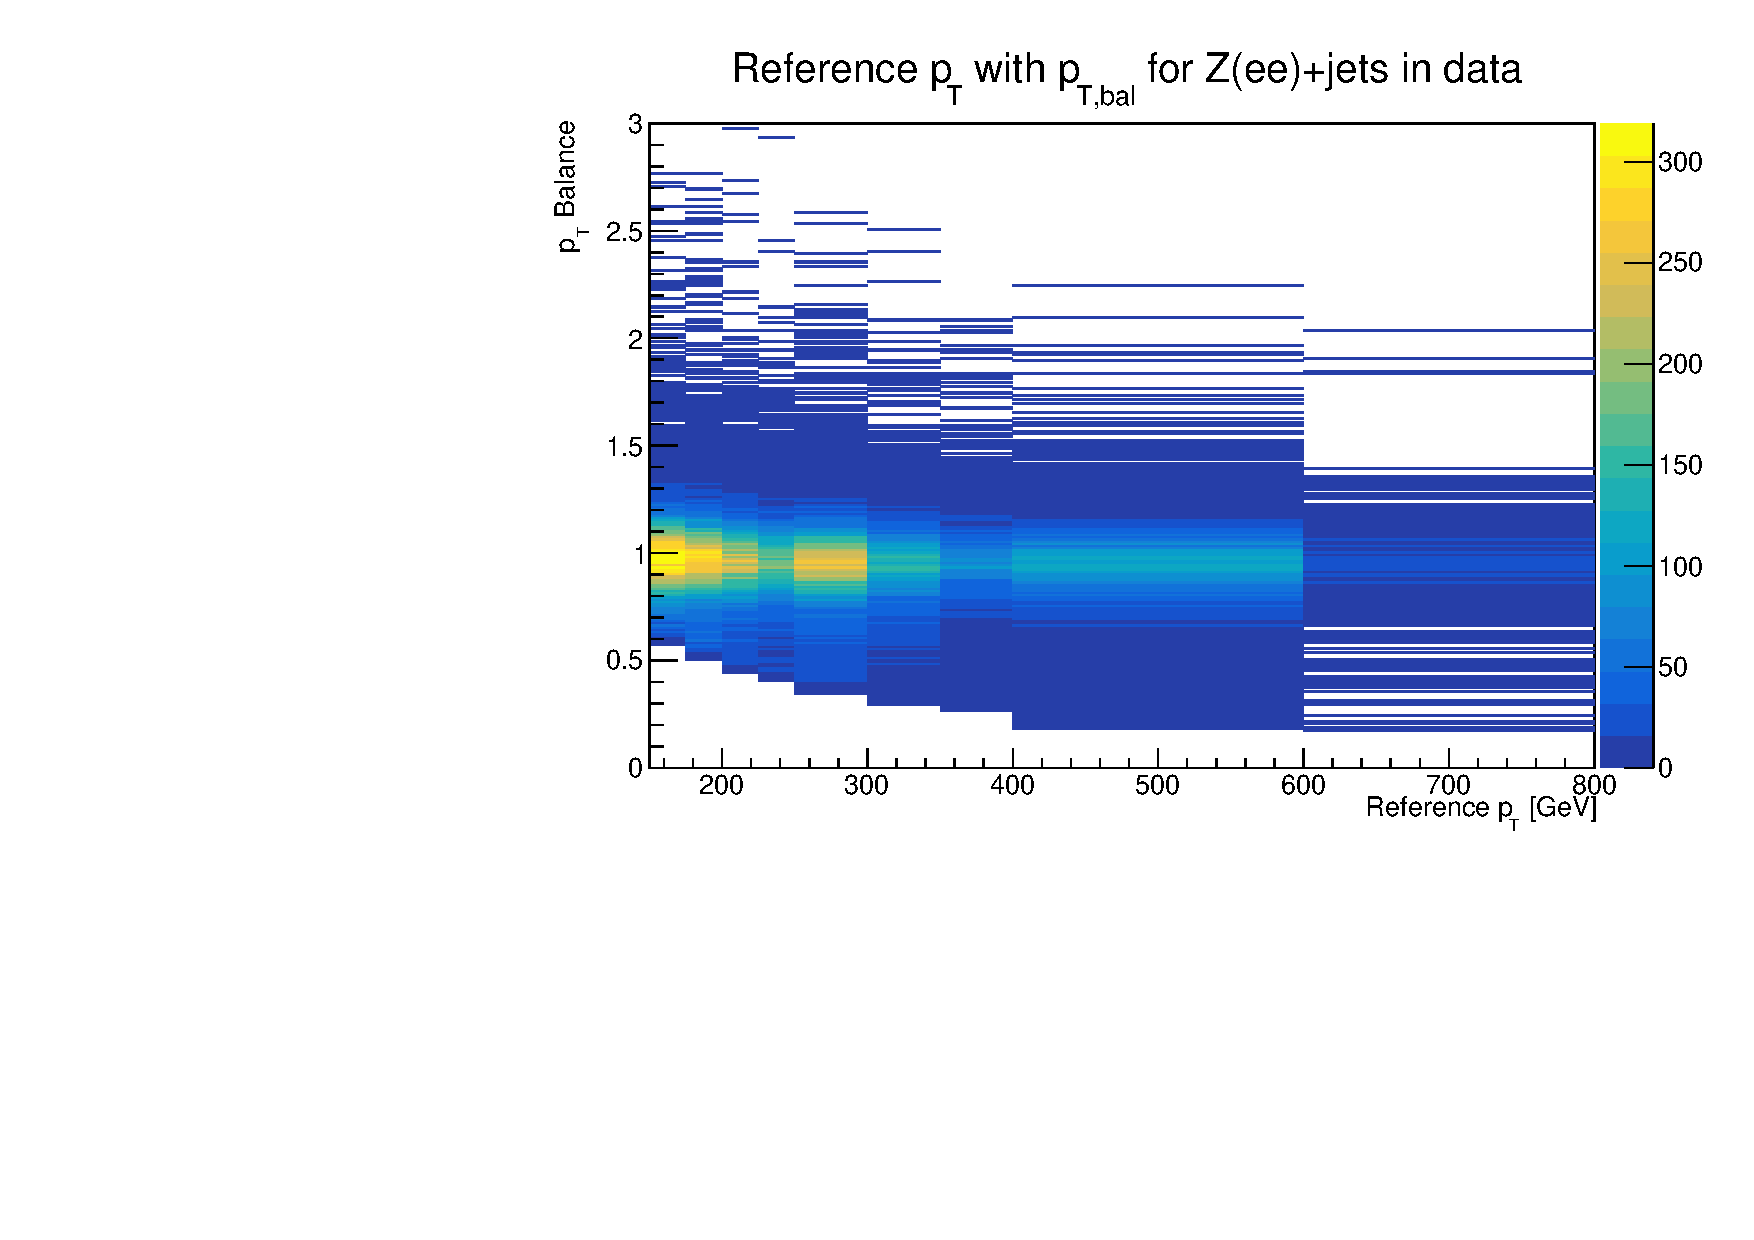
\includegraphics[width=0.8\textwidth]{plots/insitu/Response2D_Data_Zee.pdf}
    \caption{\ptref with \ptbal for \zee events in data. The response distributions in bins of \ptref are y-axis slices of this 2D histogram.\label{fig:insitu:2dhistzeedata}}
\end{figure}

The 2D histogram is sliced in bins of \ptref, and the average response \rdb is determined from the mean of a Gaussian fit. The error on the mean is used to quantify the statistical uncertainty on \ptbal. %%%FROM HERE%%% 

Before performing the fit, each \ptref distribution is uniformly re-binned in accordance to Scott's normal reference rule \cite{Insitu:scottsrule}, which states that the bin width should be as close as possible to $\frac{3.5\sigma_{\text{hist}}}{\sqrt[3]{N}}$ ($\sigma_{\text{hist}}$ is the standard deviation of the histogram and $N$ is the number of events). After re-binning, a Gaussian distribution is fit using a minimum log-likelihood method, where the likelihood is built assuming a Poisson probability density function for each bin \cite{Insitu:likelihoodfit}. This fit is performed over the range $x_{\text{max}}\pm\frac{x_{\text{max}}}{8}$, where $x_{\text{max}}$ is the $x$ value corresponding to the bin with the maximum histogram content. After the fit, the range is adjusted to $\mu_{\text{fit}}\pm1.6\sigma_{\text{fit}}$, where $\mu_{\text{fit}}$ is the mean of the Gaussian, and $\sigma_{\text{fit}}$ is the width\footnote{The reason for not fitting over the entire histogram range is because of the non-Gaussian nature of the low \ptbal tail. This non-Gaussian tail comes about due to the 100\GeV cut on the large-R jet \pt, and the maximum value of the \ptref bin. For example, in the 150-175\GeV bin, the minimum value \ptbal can take is $100/175=0.57$. There is no such upper limit for \ptref, leading to a slight bias at low \ptref}. In this way approximately 90\% of the events contribute to the fit. A second Gaussian fit is then performed over the new fit range, now using $\chi^2$ minimisation. The fit range is adjusted again in the same way, and a third Gaussian fit is performed, again using $\chi^2$ minimisation. This fit method results in lower reduced $\chi^2$ values than a single fit with a static fit range \cite{Insitu:JetResponseFitter}.

The response fits are shown for data in the electron channel in Figure \ref{fig:insitu:zeedatafits} and the muon channel in Figure \ref{fig:insitu:zmmdatafits}. See Appendix \ref{sec:appendix:responsefits} for the Gaussian fits from simulated events for both channels. 
\begin{figure}[t]
    \centering
    %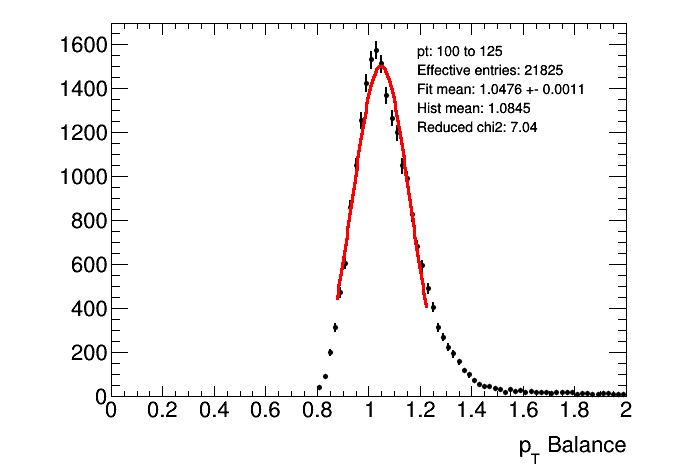
\includegraphics[width=0.31\textwidth]{plots/insitu/fits_data_zee_nominal/Zeejet_Nominal_Bin0.png}
    %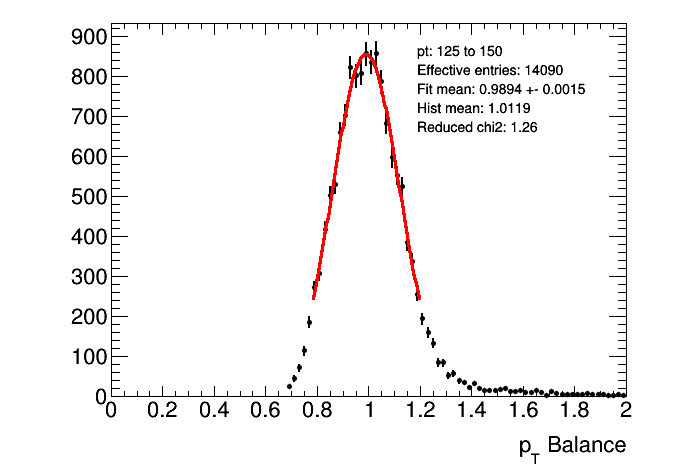
\includegraphics[width=0.31\textwidth]{plots/insitu/fits_data_zee_nominal/Zeejet_Nominal_Bin1.png}
    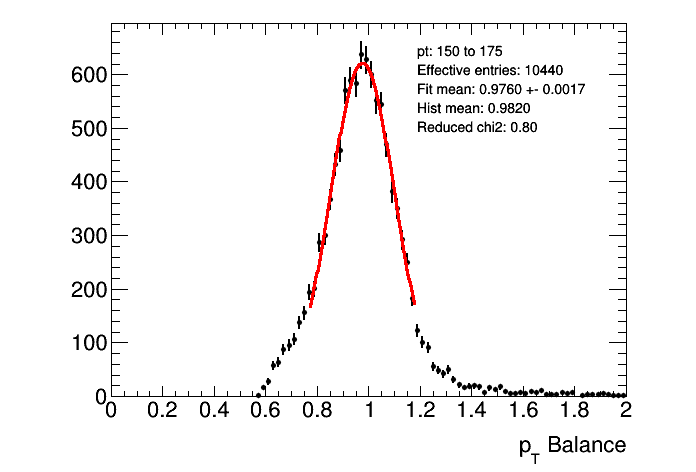
\includegraphics[width=0.31\textwidth]{plots/insitu/fits_data_zee_nominal/Zeejet_Nominal_Bin2.png}
    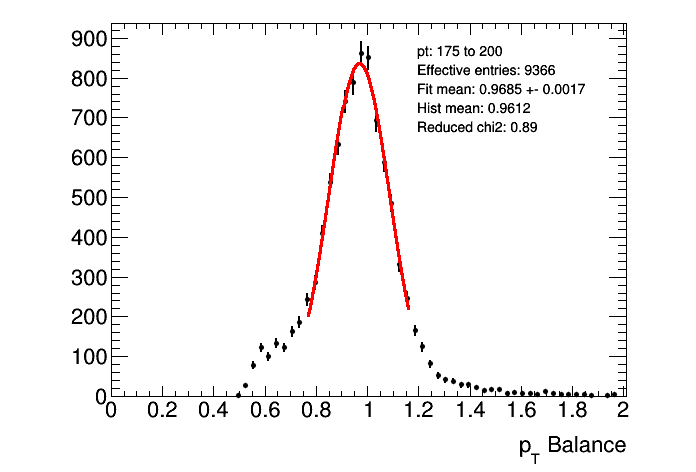
\includegraphics[width=0.31\textwidth]{plots/insitu/fits_data_zee_nominal/Zeejet_Nominal_Bin3.png}
    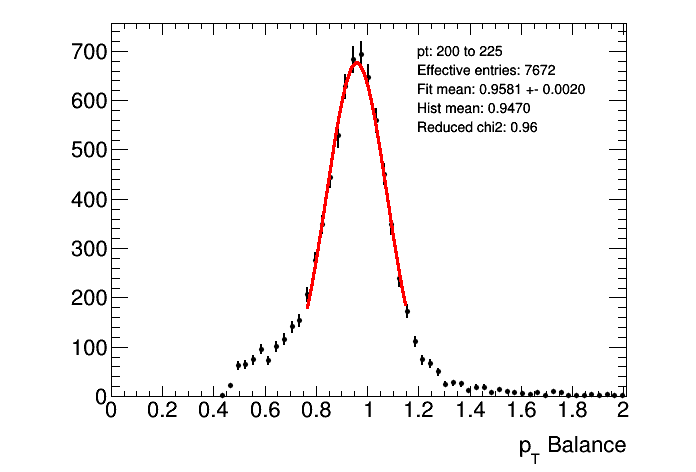
\includegraphics[width=0.31\textwidth]{plots/insitu/fits_data_zee_nominal/Zeejet_Nominal_Bin4.png}
    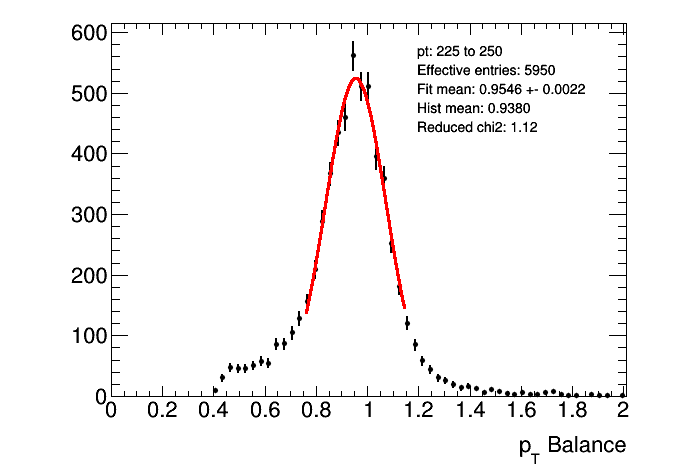
\includegraphics[width=0.31\textwidth]{plots/insitu/fits_data_zee_nominal/Zeejet_Nominal_Bin5.png}
    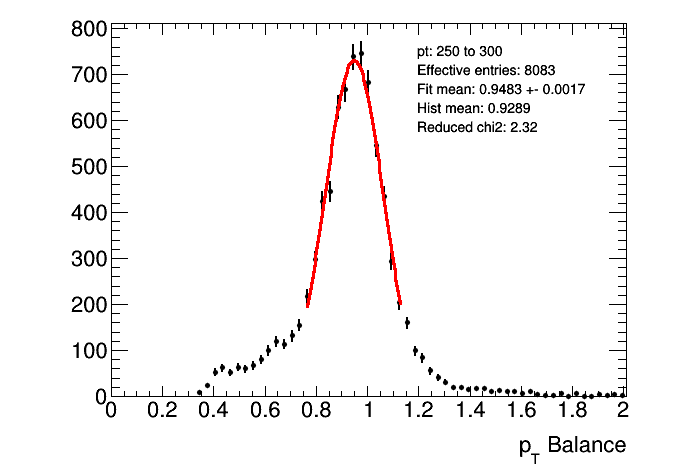
\includegraphics[width=0.31\textwidth]{plots/insitu/fits_data_zee_nominal/Zeejet_Nominal_Bin6.png}
    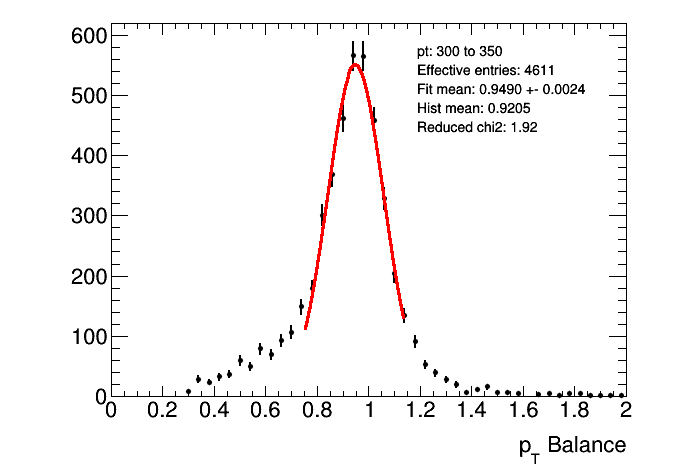
\includegraphics[width=0.31\textwidth]{plots/insitu/fits_data_zee_nominal/Zeejet_Nominal_Bin7.png}
    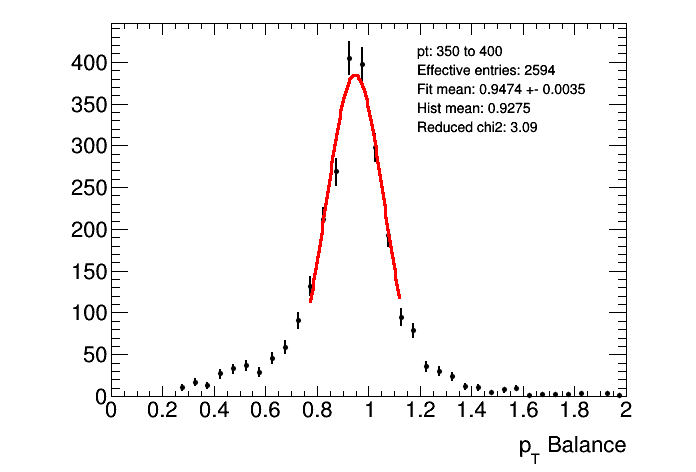
\includegraphics[width=0.31\textwidth]{plots/insitu/fits_data_zee_nominal/Zeejet_Nominal_Bin8.png}
    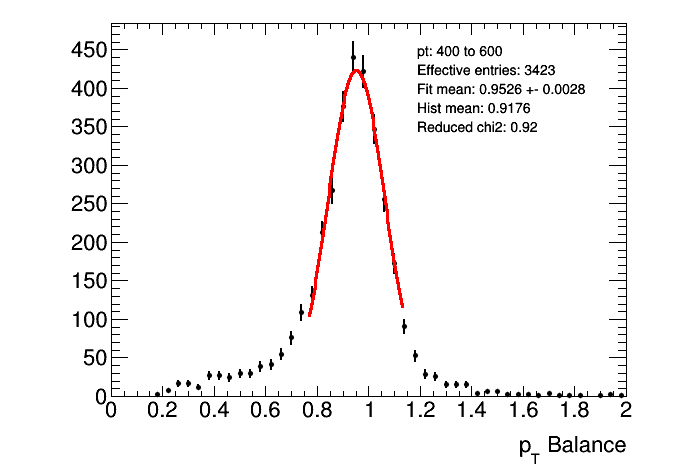
\includegraphics[width=0.31\textwidth]{plots/insitu/fits_data_zee_nominal/Zeejet_Nominal_Bin9.png}
    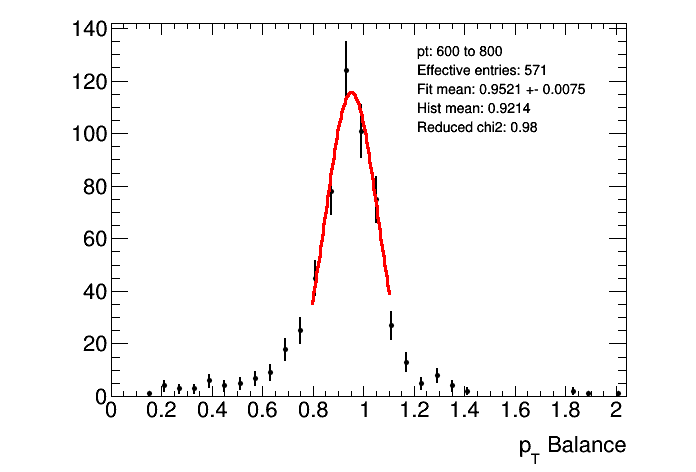
\includegraphics[width=0.31\textwidth]{plots/insitu/fits_data_zee_nominal/Zeejet_Nominal_Bin10.png}
    \caption{Gaussian fits to \ptbal in slices of \ptref in the electron channel. The $y$-axis shows the number of events per bin.\label{fig:insitu:zeedatafits}}
\end{figure}

\begin{figure}[t]
    \centering
    %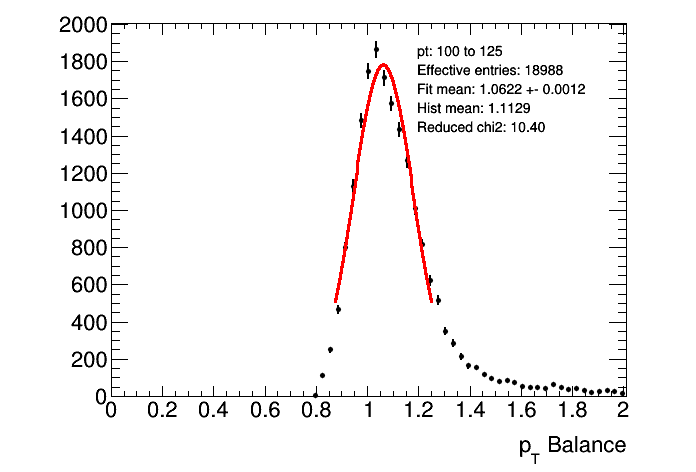
\includegraphics[width=0.31\textwidth]{plots/insitu/fits_data_zmm_nominal/Zmmjet_Nominal_Bin0.png}
    %\includegraphics[width=0.31\textwidth]{plots/insitu/fits_data_zmm_nominal/Zmmjet_Nominal_bin1.png}
    \includegraphics[width=0.31\textwidth]{plots/insitu/fits_data_zmm_nominal/Zmmjet_Nominal_bin2.png}
    \includegraphics[width=0.31\textwidth]{plots/insitu/fits_data_zmm_nominal/Zmmjet_Nominal_bin3.png}
    \includegraphics[width=0.31\textwidth]{plots/insitu/fits_data_zmm_nominal/Zmmjet_Nominal_bin4.png}
    \includegraphics[width=0.31\textwidth]{plots/insitu/fits_data_zmm_nominal/Zmmjet_Nominal_bin5.png}
    \includegraphics[width=0.31\textwidth]{plots/insitu/fits_data_zmm_nominal/Zmmjet_Nominal_bin6.png}
    \includegraphics[width=0.31\textwidth]{plots/insitu/fits_data_zmm_nominal/Zmmjet_Nominal_bin7.png}
    \includegraphics[width=0.31\textwidth]{plots/insitu/fits_data_zmm_nominal/Zmmjet_Nominal_bin8.png}
    \includegraphics[width=0.31\textwidth]{plots/insitu/fits_data_zmm_nominal/Zmmjet_Nominal_bin9.png}
    \includegraphics[width=0.31\textwidth]{plots/insitu/fits_data_zmm_nominal/Zmmjet_Nominal_bin10.png}
    \caption{Gaussian fits to \ptbal in slices of \ptref in the muon channel. The $y$-axis shows the number of events per bin.\label{fig:insitu:zmmdatafits}}
\end{figure} %%%HERE%%%

The 18 Gaussian fits in Figures \ref{fig:insitu:zeedatafits} and \ref{fig:insitu:zmmdatafits} qualify the average jet response, \rdb, as a function of \ptref. However, since the final in-situ calibration is applied to large-R jets, the \ptref values need to be mapped to \ptJ. To derive the mapping, a 2D histogram of \ptref vs \ptJ is produced. For a given \ptref slice, the \ptJ bin center is given by the histogram mean over the range $[0.4p_{\text{T,ref},i}^{\text{low}},1.6p_{\text{T,ref},i}^{\text{high}}]$, where $p_{\text{T,ref},i}^{\text{low}}$ and $p_{\text{T,ref},i}^{\text{high}}$, are the lower and upper bin edges for bin $i$ of \ptref, respectively. The $\ptJ$ midpoint values for each \ptref bin are shown in Figure \ref{fig:insitu:mapping}.
\begin{figure}[t]
\centering
\includegraphics[width=\textwidth]{plots/insitu/Sherpa.all_MappingVsPt_WIP.pdf}    
\caption{\ptref with midpoint \ptJ values on a log scale. The horizontal bars represent the bin edges of the original \ptref binning. The black dots in the top canvas shows the $\ptJ$ midpoints for a given \ptref slice. The diagonal line is $\ptJ = \ptref$. The ratio plot shows the ratio of the midpoints of the \ptJ bins with the midpoints of the \ptref bins. It is evident from this plot that the bins at higher \ptref have a larger correction than the bins at lower \ptref.\label{fig:insitu:mapping}}
\end{figure}

%\clearpage
\section{Systematic Uncertainties}

Systematic uncertainties in the in-situ correction arise from the reconstruction and calibration of the leptons, the choice of event generator used to calculate the double ratio $c$, the JVT working point, and the variations in the event selection criteria (given in Table \ref{tab:evsel_insitu}). JES and JER systematic uncertainties on the small-R jet used in the radiation veto, and lepton reconstruction, ID, isolation and trigger efficiency scale factors, are not considered. These uncertainties were found to be negligible in previous large-R jet calibration efforts at ATLAS \cite{Atlas:largercali}. The statistical uncertainties from the number events in data, and the number of simulated events are included in the final uncertainty. 

There are 64 independent sources of uncertainty which contribute to the electron energy scale variations. These include uncertainties in the material upstream of the calorimeter, cell readout non-linearity, transitions between higher and lower gains in the EM calorimeter, presampler calibration, intercalibration of first and second accordion layers, \zee energy scale calibration, pileup modelling, and lateral shower shape development \cite{Atlas:egamcal_fullrun2}. 

The sources of uncertainty contributing to the electron energy resolution are: shower and sampling variations in the calorimeter, fluctuations in the energy loss upstream of the calorimeter, electronics and pileup noise, and residual non-uniformities affecting the measurement of the energy in the data \cite{Atlas:egamcal_run2}. For the muon \pt scale and resolution uncertainties, the sources include: the $J/\psi\rightarrow\mu^+\mu^-$ and \zmm fits, reweighting simulated $Z$ samples to improve agreement with data, decay and final state radiation modelling, $J/\psi/Z$ \pt template range, $J/\psi/Z$ mass binning, $J/\psi/Z$ mass window, $J/\psi$ alternate background parametrisation function, the closure test, and statistical uncertainty \cite{Insitu:muoncal}.

%
%\begin{itemize}
%    \item Uncertainties in the material upstream of the calorimeter,
%    \item Cell readout non-linearity,
%    \item Transitions between higher and lower gains in the EM calorimeter,
%    \item Presampler calibration,
%    \item Intercalibration of first and second accordion layers,
%    \item \zee energy scale calibration uncertainties,
%    \item Pileup modelling,
%    \item Lateral shower shape development.
%\end{itemize}
%The contributions to the electron energy resolution are \cite{Atlas:egamcal_run2}:
%\begin{itemize}
%    \item Shower and sampling variations in the calorimeter,
%    \item Fluctuations in the energy loss upstream of the calorimeter,
%    \item Uncertainties from the electronics and pileup noise,
%    \item Residual non-uniformities affecting the measurement of the energy in the data.
%\end{itemize}
%The sources of uncertainty contributing to the muon \pt scale and resolution are \cite{Insitu:muoncal}:
%\begin{itemize}
%    \item Uncertainties from the $J/\psi\rightarrow\mu\mu$ and $Z\rightarrow\mu\mu$ fits,
%    \item Uncertainties from reweighting simulated $Z$ samples to improve agreement with data,
%    \item Decay and final state radiation modelling,
%    \item $J/\psi/Z$ \pt template range,
%    \item $J/\psi/Z$ mass binning,
%    \item $J/\psi/Z$ mass window,
%    \item $J/\psi$ alternate background parametrisation function,
%    \item Closure test and statistical uncertainty.
%\end{itemize} 
 Up and down variations in the each of the scale and resolution systematic uncertainties are propagated independently through the analysis chain and are later symmetrised (with the exception of MC modelling and JVT). Systematic variations in the electron and muon calibration are applied only to simulation when calculating the systematic uncertainty on the double ratio $c$. Each source of uncertainty for the $e/\mu$ scale and resolution is considered as fully correlated across $\eta$ and $\pt$, and are all added in quadrature (independently for electrons, and MS and ID components for muons)

The MC modelling uncertainty is evaluated by performing the response measurements separately for the \SHERPA and \POWPY samples. The double ratio is calculated for both response measurements, and the difference between the nominal values defines the uncertainty. Sherpa is chosen as the nominal MC generator because a significantly larger degree of mismodelling is seen in the Powheg-Pythia samples as a function of jet \pt as shown in Figure \ref{fig:insitu:mismodelling}.
\begin{figure}[t]
\centering
\begin{subfigure}[b]{0.48\textwidth}
    \centering
    \includegraphics[width=\textwidth]{plots/insitu/Zeejet_Nominal_jetPt_jet0_logY.pdf}
    \caption{}
    \label{fig:insitupt:a}
\end{subfigure}
\hfill
\begin{subfigure}[b]{0.48\textwidth}
    \centering
    \includegraphics[width=\textwidth]{plots/insitu/Zeejet_Nominal_refPt_logY.pdf}
    \caption{}
    \label{fig:insitupt:b}
\end{subfigure}
\caption{Data to MC distributions for the \ptJ (a) and \ptref (b). The MC distributions are normalised to the data distribution. It is clear that there is a large degree of mismodelling in the \POWPY MC sample which cannot be explained by the lack of an in-situ calibration, as this is of the order of a few \%. For this reason the \POWPY sample is only used to quantify a systematic modelling uncertainty of $c$, and is not used in the calculation of the nominal value.\label{fig:insitu:mismodelling}}%From MJB documentation: NLO Powheg+Pythia 8 was known to have an issue matching jets with the parton shower, leading to poor modeling of all jet pT, as well as the recoil system pT, as seen in Figure 2 a, c, d.
\end{figure}

For uncertainties associate with JVT, the \textit{Medium} working point is used. The default \textit{Tight} working point is defined by the threshold $JVT > 0.5$, and the \textit{Medium} working point is $JVT > 0.2$. The cut values refer to the output values of the JVT likelihood-based discriminant derived from simulated dijet events \cite{Insitu:JVT}.

Systematic variations in the event selection criteria are carried out to test the assumption of a $2\rightarrow2$ topology. The $\Delta\phi(J,Z)$ variations are defined by varying the default selection by $\pm0.1$ radians. Table \ref{tab:evsel_insitu} gives the variations in the radiation veto. Event selection and JVT systematic variations are performed simultaneously in data and MC. 

Each source of uncertainty is considered as fully correlated across $\eta$ and \pt. Each uncertainty is evaluated by propagating each source through the analysis chain and calculating its effect on the double ratio, $c$. The final uncertainty is taken to be the quadrature sum of the individual uncertainties.

%The statistical uncertainties on in data and MC responses are given by the standard error on the mean of the Gaussian fits, i.e. $\sigma/\sqrt{N}$, where $\sigma$ is the fitted standard deviation, and $N$ is the number of data or MC events. The data and MC statistical uncertainties are propagated to the \rdb using error propagation for uncorrelated uncertainties.
% 1. Discuss how the e/mu/jvt uncertainties are defined and talk about up and down variations and symmetrising
% 2. Include a cutflow, NAH
% 3. Discuss the bootstrapping, show an example of the bootstrapping, maybe generator choice.

%The \textit{bootstrapping} procedure is used to evaluate the statistical significance of the systematic uncertainties.    This is done such that one can separate contributions from statistics and systematics in the following way. Consider one set MC events where, for example the Jet Energy Scale (JES), is at its nominal value and another set of events where the JES is at a slightly different value, the events remain entirely correlated, one just has a slightly different scaling for the jet energies and \pt. One of the implications of this is that if one wants to determine the statistical uncertainty \textbf{on a} systematic uncertainty (derived by subtracting the extracted yields from using nominal and varied templates), that the standard error propagation formalism cannot be used (this assumes uncorrelated uncertainties). One way to approach this problem is through the \textit{bootstrapping} procedure, where $N_{\text{bootstraps}}$ pseudo-experiments are constructed for the nominal case and for each systematic variation. These bootstraps are created by multiplying each MC event weight by a random number sampled from a unit (discrete) Poisson distribution. The bootstraps are created in such a way as to preserve the correlations between nominal bootstrap numbered $x$, and systematic bootstrap corresponding to the same number, $x$. If these correlations we not preserved, the difference between the nominal and systematic bootstraps would not just correspond to the difference due to the systematic variation, but also due to the statistical variations between each bootstrap, hence the resulting statistical uncertainty would be drastically overestimated. The correlations are preserved by choosing the same random number seed when sampling the unit Poisson for each nominal and systematic MC event corresponding to the same event number. $N_{\text{bootstraps}}=10000$ is determined to be sufficient for this analysis.%Since the MC and data stat uncertainties are the largest uncertainties on the measurement, it is impotartant that a sufficient number of bootstraps is used to determine these precisely. 
%
%The systematic uncertainties provide information about real changes in the response due to changes in the MC event generator, physics objects, and event selection definitions. However, the response can also change solely because a different statistically random set of events was selected. It is therefore a requirement that the systematic uncertainties should be statistically significant, i.e. there is a small probably -- less than $4.55\%$ in our case -- that the changes in the response come about solely due to random statistical fluctuations.

To prevent large statistical fluctuations in the systematic uncertainties, a \textit{bootstrapping} procedure is used to determine a statistically significant re-binning for every source of uncertainty. In this procedure, 100 bootstrap replicas are created, where each replica has a copy of the nominal 2D distribution (Figure \ref{fig:insitu:2dhistzeedata}) and each systematically varied 2D distribution. For each event in the dataset, 100 event weights are chosen by sampling a Poisson distribution with mean of one. These represent a modified set of event weights, one for each bootstrap replica. Each replica histogram is then filled with its corresponding set of event weights. The sampling of the Poisson distribution depends on a random number uniquely determined from the run and event number. In this way, nominal events, and events corresponding to systematic variations remain correlated for every replica. The nominal \rdb response values for one of the \ptref bins in data for 100 replicas is shown in Figure \ref{fig:insitu:replicas}.

%In this procedure, a pseudodataset called a ``replica'' is also filled with each event weight multiplied by an integer factor sampled from a unit Poisson distribution. 100 such replicas are filled, and the collection of replicas defines a ``bootstrap'' object. A bootstrap object is created for the nominal dataset and for each systematic variation. For each event replica, the sampling of the Poisson distribution depends on a random number uniquely determined from the run and event number. In this way, nominal events, and events corresponding to systematic variations remain correlated for every replica in the bootstrap. The bootstrapping is used to derive a statistically significant re-binning for the systematic uncertainties, it does not have a large effect on the values themselves. The distribution of fitted \rdb response values for one of the \ptref bins in data for \zee events is shown in Figure \ref{fig:insitu:replicas}.
\begin{figure}[t]
\centering
\includegraphics[width=0.8\textwidth]{plots/insitu/Nominal_response_toys_bin8.pdf}
\caption{The \rdb response derived from 100 nominal replica distributions in bin 8 of \ptref in the electron channel. Every entry in this histogram has a corresponding value for any given systematic uncertainty. By calculating the spread in the differences between these correlated values, the statistical significance of the systematic variation for a given bin can be ascertained. The $x$-axis shows \ptref and the $y$-axis shows the number of replica instances per bin.\label{fig:insitu:replicas}}
\end{figure}

The re-binning procedure works by iterating over each \ptref bin, and determining the double ratio $c$ for each replica of the systematic variation ($c_{i}^{\text{sys}}$), and for each nominal replica ($c_{i}^{\text{nom}}$). The value of the systematic uncertainty for a given replica, $i$, is then given by: 
\begin{equation}
\delta_{\text{sys},i}=\frac{c_{i}^{\text{sys}}-c_{i}^{\text{nom}}}{c_{i}^{\text{nom}}}.
\end{equation}
The statistical significance of the systematic variation is given by the ratio of the systematic uncertainty calculated from the un-fluctuated dataset, $\delta_{\text{sys}}$, and the standard deviation of the replica systematic uncertainties. The systematic uncertainty is deemed to be statistically significant if this ratio is larger than 2. If this criteria is met, the bin is kept as it was. Otherwise, the \ptref bin is combined with the next bin, and the nominal and systematic responses are re-fit with the combined bins. If the significance threshold is still not reached, the next \ptref bin is added, and the responses are subsequently re-fit. To prevent over-binning, only a maximum of 5 bins are allowed to be combined. An example of a systematic uncertainty which is rebinned (MC modelling) and one which is not rebinned (electron energy scale) is shown in Figure \ref{fig:insitu:mctypescale}.

\begin{figure}[t]
\centering
\begin{subfigure}[b]{0.48\textwidth}
    \centering
    \includegraphics[width=\textwidth]{plots/insitu/mctype_WIP.pdf}
    \caption{}
    \label{fig:insitupt:a}
\label{fig:insitupt:a}
\end{subfigure}
\begin{subfigure}[b]{0.48\textwidth}
    \centering
    \includegraphics[width=\textwidth]{plots/insitu/egamma_scale_WIP.pdf}
    \caption{}
    \label{fig:insitupt:b}
\end{subfigure}
\hfill
\begin{subfigure}[b]{0.48\textwidth}
    \centering
    \includegraphics[width=\textwidth]{plots/insitu/mcchoice_sig.pdf}
    \caption{}
    \label{fig:insitupt:c}
\end{subfigure}
\begin{subfigure}[b]{0.48\textwidth}
    \centering
    \includegraphics[width=\textwidth]{plots/insitu/eescale_sig.pdf}
    \caption{}
    \label{fig:insitupt:d}
\end{subfigure}
\caption{MC modelling uncertainty on \rdb prior to the mapping to \ptJ (a). Electron energy scale uncertainties on \rdb prior to mapping to \ptJ. Statistical significance of the MC modelling uncertainty is shown in (c), and the up variation of the electron energy scale in (d). In (a), the last two bins (bins 7 and 8) were not statistically significant, but were made statistically significant with the addition of bin 6. In (b), all uncombined bins are statistically significant, and no rebinning has taken place.\label{fig:insitu:mctypescale}}%From MJB documentation: NLO Powheg+Pythia 8 was known to have an issue matching jets with the parton shower, leading to poor modeling of all jet pT, as well as the recoil system pT, as seen in Figure 2 a, c, d.
\end{figure}

%(containing 100 replicas) of the 2D histogram response histograms (Figure \ref{fig:insitu:2dhistzeedata}) are created. To create the replicas, each event weight is multiplied by a random integer sampled from a unit Poisson distribution. The Poisson distribution is sampled 100 times such as to create 100 replicas. The 100 random number seeds for each event are determined uniquely from the run and event number such that nominal events and events from systematic variations are correlated. The bootstrapping procedure does not directly affect the values of the systematic uncertainties, but is only used to derive a statistically significant rebinning.
\begin{table}[t]
    \small
    \centering
     \caption[]{Sources of uncertainty on the double ratio in the \zjets in-situ correction.}
           \begin{tabular}{ l l}
           \toprule
       Component & \multicolumn{1}{c}{Description} \\ 
           \midrule  
           $e$ E scale & 		Uncertainty in the electron energy scale \\
           $e$ E resolution & 	Uncertainty in the electron energy resolution \\
           $\mu$ \pt resolution ID & 	Uncertainty in muon \pt resolution in the ID \\
           $\mu$ \pt resolution MS & 	Uncertainty in muon \pt resolution in the MS \\
           $\mu$ \pt scale res. \& comb. & Muon \pt scale uncertainties from (residual and combined) charge-dependent corrections \\
           $\mu$ \pt scale & Uncertainty in the muon \pt scale from charge-independent corrections \\
           %Uncertainty (Sagitta) from variations in the (charge-dependent) momentum scale, based on the residual charge-dependent bias after correction; Uncertainty from variations in the (charge-dependent) momentum scale, based on combination of corrections on combined (Z-scale) and recombination of corrections \\
           MC modelling & 		Difference between MC event generators \\
           Pile-up (JVT) & 				Jet vertex tagger uncertainty \\
           $\Delta \phi$ &		Variation of $\Delta \phi$ between the jet and $Z$ boson \\
           Small-R jet veto &		Radiation suppression through second-jet veto \\
           Statistical & Total MC and data Statistical uncertainty \\
           \bottomrule
       \end{tabular}
       \label{tab:jes_uncertainties}
   \end{table}

%\clearpage
\section{Results\label{sec:insitu:results}}
The responses \rdb for the electron and muon channels after the \ptref to \ptJ mapping are shown in Figure \ref{fig:nominalfitbalance}. The systematic uncertainties on the double ratio with \ptref prior to symmetrising are shown in Figure \ref{fig:insitu:ptrefsysts}. The final systematic uncertainties on \ptJ are shown in Figure \ref{fig:insitu:systs}. From the response distribution it is evident that the jets require a quasi-flat 2\% correction in both electron and muon channels. The size of this correction is very similar to the one derived for large-R LCTopo jets \cite{Atlas:largercali}. However, the shape of the \rdb distribution is very different in that there is a clear up-turn at low \ptJ, this was not seen for large-R LCTopo jets. This upturn was seen in all the in-situ calibrations (\gamma+jets, \zjets, and MJB) for the UFO large-R in-situ JES measurements \cite{Insitu:combination}. 

\begin{figure}[t]
\centering
\begin{subfigure}[b]{0.70\textwidth}
    \centering
    \includegraphics[width=\textwidth]{plots/insitu/Zeejet_response_WIP.pdf}
    \caption{\vspace{20pt}}
    \label{fig:insitufitbal:a}
\end{subfigure}
\hfill
\begin{subfigure}[b]{0.70\textwidth}
    \centering
    \includegraphics[width=\textwidth]{plots/insitu/Zmmjet_response_WIP.pdf}
    \caption{}
    \label{fig:insitfitbal:b}
\end{subfigure}
\caption{Direct balance response, \rdb, and the double ratio ``MC/Data'' (1/$c$), with leading large-R jet pt \ptJ. The error bars only show statistical uncertainties. (a) shows the response for the electron channel, and (b) shows the muon channel. In the final calibration, the final bin in the muon channel is omitted due to large statistical uncertainty on the response. This comes about because fewer events are selected in the muon channel (also seen in MPF results \cite{Insitu:MPFresults}).\label{fig:nominalfitbalance}}%From MJB documentation: NLO Powheg+Pythia 8 was known to have an issue matching jets with the parton shower, leading to poor modeling of all jet pT, as well as the recoil system pT, as seen in Figure 2 a, c, d.
\end{figure}

\begin{figure}[t]
\centering
\begin{subfigure}[b]{\textwidth}
    \centering
    \includegraphics[width=\textwidth]{plots/insitu/unc_ptref_zee_WIP.pdf}
    \caption{\vspace{20pt}}
\end{subfigure}
\hfill
\begin{subfigure}[b]{\textwidth}
    \centering
    \includegraphics[width=\textwidth]{plots/insitu/unc_ptref_zmm_WIP.pdf}
    \caption{}
\end{subfigure}
\caption{Uncertainties on the double ratio in the electron (a) and muon (b) channels with \ptref before the mapping to \ptJ, and before symmetrising of the uncertainties. For uncertainties which do not have a down variation (for example statistical, MC modelling), a down variation is plotted by simply inverting the sign, this is done only for aesthetic reasons.\label{fig:insitu:ptrefsysts}}
\end{figure}

\begin{figure}[t]
\centering
\begin{subfigure}[b]{\textwidth}
    \centering
    \includegraphics[width=\textwidth]{plots/insitu/systtotal_zee_WIP.pdf}
    \caption{\vspace{20pt}}
\end{subfigure}
\hfill
\begin{subfigure}[b]{\textwidth}
    \centering
    \includegraphics[width=\textwidth]{plots/insitu/systtotal_zmm_WIP.pdf}
    \caption{}
\end{subfigure}
\caption{The final uncertainties on the in-situ JES correction with \ptJ and symmetrised uncertainties in the electron (a) and muon (b) channels. Uncertainties are symmetrised by subtracting the down variations from the up variations and dividing by two.\label{fig:insitu:systs}}
\end{figure}

%\clearpage
\section{In-situ combination}

The results in Figures \ref{fig:insitu:systs} and \ref{fig:nominalfitbalance} were used in the in-situ combination \cite{Insitu:combination} to derive the precision recommendations for Athena Release-21 large-R UFO jets. In the combination, the $\eta$-intercalibration \cite{Insitu:etainterufo}, $\gamma$+jets \cite{Insitu:gamjetufo}, \zjets \cite{Insitu:zjetufo}, and MJB results \cite{Insitu:mjbufo} are combined to form the final in-situ correction factor ($c$) to the JES. The combination of all the $c$ factors and uncertainties is shown in Figure \ref{fig:insitu:combination}. 

\begin{figure}[t]
    \centering
    \includegraphics[width=0.8\textwidth]{plots/insitu/combinationplot.pdf}
    \caption{The combination of all the in-situ measurements and the final in-situ correction factor to the JES, with corresponding statistical and systematic uncertainties. The \zjets and $\gamma+$jets results are in very good agreement. These results are derived completely independently using different software packages. The last data point from the \zmmjets calibration is omitted due to poor statistical precision in this bin. The \zjets and $\gamma$+jets calibrations cover the 150-900\GeV range, and these calibrations typically have $<1\%$ total uncertainty. From around 150-200\GeV the in-situ correction is covered solely by \zjets and $\gamma$+jets measurements, and superior precision is seen in the $\gamma$+jets channel. The 150-750\GeV range is covered by all in-situ measurements. From around 200-500\GeV, the \zjets channels have the superior precision, and from 500-900\GeV the $\gamma$+jets channel provides the superior measurement. Above 900\GeV, the calibration is solely covered by the MJB measurement. The final uncertainties on the combined calibration are typically below 0.5\%. Figure taken from \cite{Insitu:combination}.\label{fig:insitu:combination}}
\end{figure}

%TODO: Muon large negative weights - mayube
%TODO: Mention bad replicas:    #Ignore obviously bad fits
% if( data_replica <= 0.01 or nominal_means_mc[ireplica] <= 0.01 or data_replica > 4 or nominal_means_mc[ireplica] > 4):
%TODO: Why MC only for CP systematics? Maybe
%TODO: Why muon multiplicity less. Investigate cutflows
%\clearpage
\section{Small-R In-situ Calibration Cross-check}
As an additional cross-check for the small-R EMPflow \zjets in-situ calibration, the InsituBalance software framework was used to derive the nominal in-situ calibration. This was compared with the nominal in-situ calibration derived using the software framework which is usually used for the small-R calibration in ATLAS (the MPF framework). 

\subsection{Samples, object definitions, and event selection}

The comparison was done using 2018 data in the electron channel. Small-R EMPFlow jets are used in the calibration. The 2018 dielectron trigger described in Table \ref{tab:Insitu:trigger} is used. Electrons are required to satisfy ``Loose'' ID and ``Loose'' isolation criteria. Jets are selected in the central $|\eta|<0.8$ region. Jets are calibrated up to the MC JES + GSC (Global Sequential Calibration) level using the 2019 consolidated recommendations. Electrons are calibrated used the same prescription as in Section \ref{sec:insitu:largerobj}. Jets are required to satisfy $\ptj>10\GeV$, and events are selected such that $\Delta\phi(j,Z)>2.8$. In order to reduce contamination from events with large hadronic recoil, a sub-leading jet veto is applied such that $\pt^{\text{second}}<\text{max}(20\GeV,0.1\times\ptref)$, where $\pt^{\text{second}}$ is the \pt of the sub-leading jet. The \textit{Tight} JVT working point is used for jets with $\pt<60\GeV$ and $\eta<2.4$. The only overlap removal requirement is that jets are required to satisfy $\DeltaR(j,Z)>0.2$.

\subsection{Results}

The responses agree very well between the two frameworks, as shown in Figure \ref{fig:insitu:crosscheck}. This serves as a cross-check for the small-R jet calibration, but indeed also gives confidence in the large-R calibration in that the software machinery is behaving as expected.

\begin{figure}[t]
\centering
\begin{subfigure}[b]{\textwidth}
    \centering
    \includegraphics[width=1.05\textwidth]{plots/insitu/SmallRresponse_logX_WIP.pdf}
    \caption{\vspace{20pt}\label{fig:insitu:crosscheck:a}}
\end{subfigure}
\hfill
\begin{subfigure}[b]{\textwidth}
    \centering
    \includegraphics[width=\textwidth]{plots/insitu/MPF_framework_RDB_WIP.pdf}
    \caption{\label{fig:insitu:crosscheck:b}}
\end{subfigure}
\caption{Comparison of the \rdb response between the InsituBalance software framework (a), and the MPF software framework (b) for 2018 data in the electron channel. The slight differences seen when comparing the first low \pt bins can be attributed to slightly different fit functions and fit range in the fits to determine the average response. The MPF framework response plot (b) was produced by Sahil Singh \cite{Insitu:sahilresponse}.\label{fig:insitu:crosscheck}}
\end{figure}

The slight differences between the response in Figures \ref{fig:insitu:crosscheck:a} and \ref{fig:insitu:crosscheck:b} can be attributed to differences in the fit range, fitting function, and binning of \ptbal. The InsituBalance framework uses a Gaussian fit over the fit range given by 1/8 times the maximum bin, and the MPF framework uses a modified Poisson distribution (a continuous generalisation of the Poisson distribution defined using the gamma function) with a dynamic, asymmetric \ptbal range. The was confirmed by explicitly checking the calibrated \ptref and \ptbal values for individual events in the 2018 data sample in the two software frameworks, and equivalent values were obtained. The \ptbal fits in \ptref bins for the InsituBalance framework and MPF framework are shown in Figures \ref{fig:insitu:insitubalancesmallrfits} and \ref{fig:insitu:mpfsmallrfits}, respectively. 

\begin{figure}[t]
    \centering
    \includegraphics[width=0.31\textwidth]{plots/insitu/fits_insitubalance_smallR/Zeejet_Nominal_Bin0.png}
    \includegraphics[width=0.31\textwidth]{plots/insitu/fits_insitubalance_smallR/Zeejet_Nominal_Bin1.png}
    \includegraphics[width=0.31\textwidth]{plots/insitu/fits_insitubalance_smallR/Zeejet_Nominal_Bin2.png}
    \includegraphics[width=0.31\textwidth]{plots/insitu/fits_insitubalance_smallR/Zeejet_Nominal_Bin3.png}
    \includegraphics[width=0.31\textwidth]{plots/insitu/fits_insitubalance_smallR/Zeejet_Nominal_Bin4.png}
    \includegraphics[width=0.31\textwidth]{plots/insitu/fits_insitubalance_smallR/Zeejet_Nominal_Bin5.png}
    \includegraphics[width=0.31\textwidth]{plots/insitu/fits_insitubalance_smallR/Zeejet_Nominal_Bin6.png}
    \includegraphics[width=0.31\textwidth]{plots/insitu/fits_insitubalance_smallR/Zeejet_Nominal_Bin7.png}
    \includegraphics[width=0.31\textwidth]{plots/insitu/fits_insitubalance_smallR/Zeejet_Nominal_Bin8.png}
    \includegraphics[width=0.31\textwidth]{plots/insitu/fits_insitubalance_smallR/Zeejet_Nominal_Bin9.png}
    \includegraphics[width=0.31\textwidth]{plots/insitu/fits_insitubalance_smallR/Zeejet_Nominal_Bin10.png}
    \includegraphics[width=0.31\textwidth]{plots/insitu/fits_insitubalance_smallR/Zeejet_Nominal_Bin11.png}
    \includegraphics[width=0.31\textwidth]{plots/insitu/fits_insitubalance_smallR/Zeejet_Nominal_Bin12.png}
    \caption{\ptbal distributions in small-R \zeejets in the InsituBalance software framework. The increase of \rdb at low \ptref can be attributed to the non-Gaussian nature of the low \ptref bins. This behaviour can be attributed to the 10\GeV \ptj cut.\label{fig:insitu:insitubalancesmallrfits}}
\end{figure}

\begin{figure}[t]
    \centering
    \includegraphics[width=0.31\textwidth]{plots/insitu/fits_MPF_smallR/mpf_fit_bin1.pdf}
    \includegraphics[width=0.31\textwidth]{plots/insitu/fits_MPF_smallR/mpf_fit_bin2.pdf}
    \includegraphics[width=0.31\textwidth]{plots/insitu/fits_MPF_smallR/mpf_fit_bin3.pdf}
    \includegraphics[width=0.31\textwidth]{plots/insitu/fits_MPF_smallR/mpf_fit_bin4.pdf}
    \includegraphics[width=0.31\textwidth]{plots/insitu/fits_MPF_smallR/mpf_fit_bin5.pdf}
    \includegraphics[width=0.31\textwidth]{plots/insitu/fits_MPF_smallR/mpf_fit_bin6.pdf}
    \includegraphics[width=0.31\textwidth]{plots/insitu/fits_MPF_smallR/mpf_fit_bin7.pdf}
    \includegraphics[width=0.31\textwidth]{plots/insitu/fits_MPF_smallR/mpf_fit_bin8.pdf}
    \includegraphics[width=0.31\textwidth]{plots/insitu/fits_MPF_smallR/mpf_fit_bin9.pdf}
    \includegraphics[width=0.31\textwidth]{plots/insitu/fits_MPF_smallR/mpf_fit_bin10.pdf}
    \includegraphics[width=0.31\textwidth]{plots/insitu/fits_MPF_smallR/mpf_fit_bin11.pdf}
    \includegraphics[width=0.31\textwidth]{plots/insitu/fits_MPF_smallR/mpf_fit_bin12.pdf}
    \includegraphics[width=0.31\textwidth]{plots/insitu/fits_MPF_smallR/mpf_fit_bin13.pdf}
    \caption{\ptbal distributions in small-R \zeejets in the MPF software framework. A modified Poisson distribution with a dynamic asymmetric fit range is used here.\label{fig:insitu:mpfsmallrfits}}
\end{figure}
\FloatBarrier
%-------------------------------------------------------------------------

%-------------------------------------------------------------------------
\chapter{Differential Cross-section Measurement of $W\gamma jj$ EW Production at $\sqrt{s}=13\TeV$}
\label{sec:vbswy}
This chapter describes the first differential cross-section measurement at ATLAS of the electroweak production of a W boson and a photon in association with two jets. The research detailed in this chapter is included in a paper submitted to journal and publicly available at \cite{VBSWy:VBSWy}, where the differential cross-section measurements are used to derive constraints on dimension-8 operators in the context of an effective field theory (EFT). The paper also describes the observation and fiducial cross-section measurements of this process. The CMS collaboration has previously reported the observation \cite{VBSWy:CMSVBSWy} and differential cross-section measurements of this process \cite{VBSWy:CMSdiffx}. The ATLAS paper is the first to publish constraints on the $f_{T3}$ and $f_{T4}$ operators\footnote{The dimension-8 $T$ operators are given by the different ways of contracting the SU(2) and U(1) field strength tensors, and represent anomalous quartic gauge interactions involving a $\gamma$ and a $W$, without trilinear interactions. The T3 and T4 operators were only added to dimension-8 EFT models in March 2021, and have therefore remained unconstrained by measurements prior to this analysis \cite{TtypeOperators}.} and also gives differential cross-section measurements of observables sensitive to CP-violating (CPV) Higgs and weak boson interactions. The work shown in this chapter is the authors own except when explicitly stated otherwise.
%Unfolded differential cross-sections for \ewwy production in 6 different observables are derived. These are the dijet invariant mass \mjj, dijet transverse momentum \jjpt, signed\footnote{Signed here refers to the fact that the jets are rapidity ordered before subtracting the azimuthal angles. This makes these observables parity-odd.} dijet azimuthal angle separation \jjdphi, lepton transverse momentum \leppt, signed azimuthal angle separation of the lepton and the photon \lepgamdphi, and the invariant mass of the lepton-photon system \lym. \mjj is measured for the reason that it characterises the EW measurement -- \mjj is one of the most important observables used to discriminate the QCD production mode from the EW mode in VBS/VBF processes. \ptjj probes the kinematics of the forward jet system, and is expected to be more sensitive to dim-8 EFT contributions than \mjj. The \leppt and \lym observables probe the kinematics of the central diboson system. %The mass of this system has been shown to be very sensitive to dim-8 EFT contributions in other VBS/VBF analyses \textcolor{red}{citation needed}. 

Unfolded differential cross-sections for \ewwy production are measured for 6 different observables. These are the dijet invariant mass \mjj, dijet transverse momentum \jjpt, signed dijet azimuthal angle separation \jjdphi, lepton transverse momentum \leppt, signed azimuthal angle separation of the lepton and the photon \lepgamdphi, and the invariant mass of the lepton-photon system \lym. The signed nature of the angular observables refers to the fact that the objects are rapidity ordered before subtracting the azimuthal angles. i.e. 
\begin{equation}
  \Delta\phi_{ij}=\phi^i_f-\phi^j_b, \hspace{5pt}\text{where}\hspace{5pt} y^i_f>y^j_b.
\end{equation}
The dijet invariant mass is one of the most important observables used to discriminate the strong production mode from the EW mode in VBS/VBF processes, in this way \mjj characterises the VBS measurement. The dijet transverse momentum probes the kinematics of the forward jet system. Preliminary EFT studies showed that \ptjj is expected to be more sensitive to dim-8 EFT contributions than \mjj. The \leppt and \lym observables probe the kinematics of the central diboson system. %The mass of this system has been shown to be very sensitive to dim-8 EFT contributions in other VBS/VBF analyses \textcolor{red}{citation needed}. 
Finally, the angular observables \jjdphi and \lepgamdphi are expected to be sensitive to CPV gauge couplings contributing to the $WW\gamma\gamma$ and $WW\gamma Z$ vertices. The \ewwy differential cross-section paper \cite{VBSWy:VBSWy} does not publish limits on these couplings as they still need to be included in EFT models in MC event generators, but the published results may help future analyses looking to derive these limits. 

\section{Signal and Background Processes}

%The nominal sample for \ewwy production is generated using \MGNLO (v.2.6.5), with LO matrix-element (ME) accuracy in perturbative QCD, where the \NNPDFlo PDF set is used in the calculation of the matrix element. The ME-level final state is interfaced with \PYTHIA (v8.240) with dipole recoil turned on for generating the parton shower (PS) and UE, using the A14 tuned parameter set for the modelling of non-perturbative effects. \EVTGEN (v1.6.0) is used for the properties of b- and c- hadron decays. An additional \ewwy sample is generated using \SHERPA2.2.12, with LO matrix element accuracy, where the \NNPDF PDF set is used, where the tuned parameter set used in the PS, UE, and hadronisation is default one developed by the \SHERPA authors. The ME calculation is performed for up to one parton using the internal ME generator \COMIX, and the ME is merged with parton showers for events with two or three partons using the \MEPSatLO prescription. All partons are treated as massless at the ME calculation, and massive in the parton shower, and diagrams involving initial state b quarks are explicitly excluded in the ME calculation, as these diagrams are covered by seperate single-top MC samples\footnote{With this setup, diagrams involving the t-channel exchange of a $Z$-boson via a b-quark are excluded from the analysis. Seperate studies have shown that this has a negligible impact. \textcolor{red}{STILL NEEDS TO BE VERIFIED}}. The parton showering is conducted by \CSShower, which is based on Catani-Seymour dipole factorisation.

\subsection{Signal}

The nominal sample for the EW production mode of $l\nu\gamma$jj (referred to as \ewwy in this chapter) is generated using \SHERPA2.2.12 \cite{Insitu:sherpa,Insitu:sherpa22}, with LO matrix element accuracy, where the \NNPDF PDF set \cite{Insitu:nnpdf} is used, and the tuned parameter set used in the parton shower (PS), underlying event (UE), and hadronisation is the default one developed by the \SHERPA authors. The ME calculation is performed for up to three partons in the finals state using the internal ME generator \COMIX \cite{Insitu:comix}, and the ME is merged with the PS for events using the \MEPSatLO prescription \cite{Insitu:meps}. All partons are treated as massless in the ME calculation, and massive in the PS, and diagrams involving initial state $b$-quarks are explicitly excluded in the ME calculation, as these diagrams are covered by separate single-top MC samples\footnote{With this setup, diagrams involving the t-channel exchange of a $Z$-boson via a b-quark are excluded from the analysis. Separate studies have shown that this has a negligible impact.}. The PS is conducted by \CSShower \cite{Insitu:csshower}, which is based on Catani-Seymour dipole factorisation \cite{Insitu:csalgorithm}. 

An additional \ewwy sample is generated using \MGNLO (v.2.6.5) \cite{VBSWy:madgraph}, with LO matrix-element (ME) accuracy in perturbative QCD, where the \NNPDFtwolo \cite{Insitu:nnpdf} PDF set is used in the calculation of the ME. The ME calculation is performed for two partons in the final state. The ME-level final state is interfaced with \PYTHIA (v8.240) \cite{Insitu:pythia} with dipole recoil turned on for generating the PS and UE, using the A14 \cite{VBSWy:a14} tuned parameter set for the modelling of non-perturbative effects. \EVTGEN (v1.6.0) \cite{Insitu:evtgen} is used for the properties of $b$- and $c$-hadron decays. The \SHERPA sample has 4783000 total events, whereas the \MGNLO sample has 5013000 total events. The \SHERPA sample is used as the nominal MC sample since the ME calculation is performed for up to three partons, compared to 2 partons (i.e. no extra emissions) in the \MGNLO sample.

It is worth commenting on the fact that LO samples are used for the simulations of the signal process. The current state-of-the-art for the MCnet MC generators are LO-merged samples, such as the \SHERPA \ewwy sample used in this analysis. The NLO calculation for $V\gamma jj$ processes is extremely challenging because of the interference with the strong $V\gamma jj$ process and the presence of infrared singularities from NLO correction to both the electroweak and strong diagrams \cite{VBSWy:VBSNLO,VBSWy:MCNetVBSNLO}. 
%The choice of the \SHERPA sample as the nominal one is based on the fact that the ME is calculated with up to three partons, compared to two partons for the \MGNLO sample.
\subsection{Backgrounds}

\subsubsection{Strong $W\gamma$jj}
The nominal irreducible background sample for the strong production mode of $l\nu\gamma$jj (referred to as \qcdwy in this chapter) is generated using \SHERPA2.2.11 \cite{Insitu:sherpa,Insitu:sherpa22}. The sample is produced with NLO accurate MEs for up to one parton in the final state, LO accuracy MEs for up to 3 partons in the finals state are calculated with \AMEGIC \cite{VBSWy:amegic} and \COMIX \cite{Insitu:comix}. Partons are treated as massless in the ME calculation, and massive in the PS. The PS is conducted with \CSShower \cite{Insitu:csshower}. The matrix elements are matched to the PS, and different jet multiplicities are merged using the CKKW matching procedure \cite{Insitu:ckkw1,Insitu:ckkw2}, which is extended to NLO accuracy using the \MEPSatNLO \cite{Insitu:meps} prescription. The \NNPDF \cite{Insitu:nnpdf} PDF set is used and the dedicated set of tuned parameters for the PS is developed by the \SHERPA authors. 

An alternate \qcdwy background sample is generated using \MGNLO (v2.8.1) \cite{VBSWy:madgraph} with NLO ME accuracy up to one parton in the final state. The \NNPDF PDF set is used in the calculation. The partonic final state is interfaced with \PYTHIA (v8.244) \cite{Insitu:pythia}, and the A14 \cite{VBSWy:a14} set of tuned parameters is used for PS, hadronisation and UE activity. \EVTGEN (v1.7.0) \cite{Insitu:evtgen} is used for the properties of $b$- and $c$-hadron decays.

118997000 events were generated for the \MGNLO sample, and 116239203 for the \SHERPA sample. The \SHERPA sample is chosen as the nominal MC sample. This choice is made because of the superior statistical precision of the expected number of events after the event selection described in Section \ref{sec:vbswy:evsel}. By comparing the statistical uncertainties on the total expected yields calculated using $\sqrt{\sum_iw_i^2}$, where $w_i$ are the MC event weights, the statistical precision of the \SHERPA sample was found to be 2.3 times better. The improved statistical precision arises due to a larger number of negative weights in \MGNLO.% The improved statistical precision results in lower statistical uncertainties on the extracted signal and improved statistical resolution of the systematic uncertainties. This is described in Section \ref{sec:vbswy:extraction_uncertainties}.

\subsubsection{Interference Between Strong and EW $W\gamma$jj}

In the calculation of the inclusive cross-section of W$\gamma$jj production, the electroweak and the strong scattering amplitudes can interfere. This interference is quantified in the matrix-element squared at LO as 
\begin{equation} 
|\mathcal{M}|^2 = |\mathcal{M}_{\text{EW}} + \mathcal{M}_{\text{QCD}}|^2 = |\mathcal{M}_{\text{EW}}|^2+|\mathcal{M}_{\text{QCD}}|^2+2Re(\mathcal{M}_{\text{EW}}^*\mathcal{M}_{\text{QCD}}),
\end{equation}
where $\mathcal{M}_{\text{EW}}$ and $\mathcal{M}_{\text{QCD}}$ represent the matrix elements for \ewwy and \qcdwy production, and the last term corresponds to the interference contribution. The interference must be modelled to understand its impact relative to the \ewwy differential cross-section as a function of the measurement observables.

The interference sample was modelled at LO ME accuracy using \MADGRAPH5, which was interfaced with \PYTHIA (v8.244) for PS, hadronisation, and UE activity. \EVTGEN (v1.7.0) was used for the properties of $b$- and $c$-hadron decays. This sample was generated by the author. More details about the generation of the sample and truth-level validations studies are shown in Section \ref{sec:vbswy:interference}.

\subsubsection{Prompt Backgrounds}
Backgrounds where the final state comprises at least two jets, a prompt lepton, and a prompt photon are referred to as prompt backgrounds. These include the production of top quarks in association with a prompt photon, as well as $Z\gamma$jj production.

The simulations of top backgrounds consist of:
\begin{itemize}
  \item $tt\gamma$ production. This sample is produced at LO ME accuracy. The all-hadronic $t\bar{t}$ decays are not included in this sample.
  \item $tq\gamma$, which is the t-channel production of a single top quark in association with a prompt photon, a $b-$jet, and one additional jet. This sample is produced at NLO accuracy. The s-channel diagrams have a negligible contribution since they produce two $b$-jets in the final state, and a $b$-jet veto is applied in the analysis. 
  \item $tW\gamma$ production, where the $W$ decays either hadronically or leptonically, and the photon comes from radiation off a $t$, $W$ or from their decay products. The sample is produced at LO accuracy. Diagrams where the photon is radiated from the initial state are highly suppressed as these involve additional heavy fermion internal lines.
\end{itemize}

All of the top background samples are simulated with the same event generation, showering, and hadronisation setup. They are generated with \MGNLO for the ME calculation, where the \NNPDFtwolo PDF set is used. The ME-level final state is interfaced with \PYTHIA for hadronisation, showering and UE activity, and the A14 set of tuned parameters is used. \EVTGEN is used for the properties of $b$- and $c$-hadron decays. 

The $Z\gamma$ backgrounds consist of:
\begin{itemize}
  \item Strong-$Z\gamma$jj production, which include separate samples for $e,\mu,\tau,\nu$ channels. MEs are calculated with \SHERPA 2.2.11 at NLO QCD accuracy for up to one additional parton, and LO accuracy for up to three additional partons.
  \item EW-$Z\gamma$jj production with a t-channel requirement to suppress triboson final states. The ME is calculated with \SHERPA 2.2.12 at LO accuracy for up to one additional parton. Diagrams with initial state $b$-quarks are explicitly excluded. 
\end{itemize}
The treatment of parton shower, hadronisation and underlying event is the same as the $W\gamma$jj samples. The \NNPDF PDF sets are used.
\subsubsection{Non-prompt backgrounds}
Background events can arise from non-prompt leptons or photons in association with jets. Additionally, electrons can be mis-reconstructed as photons (referred to as \efakey backgrounds), and jets can be mis-reconstructed as photons (\jfakey) or leptons (\jfakee, \jfakemu). The contributions from these backgrounds are estimated using data-driven methods as described in Section \ref{sec:vbswy:nonprompt}. %These backgrounds are collectively referred to as non-prompt backgrounds in this chapter. The MC samples used for the non-prompt background estimates are 
%\begin{itemize}
%  \item $W$+jets -- used in \jfakey validation.
%  \item $Z$+jets -- used in \jfakey validation, \efakey estimate.
%  \item $tW$ -- used in \efakey estimate.
%  \item $t\bar{t}$ -- used in \efakey estimate.
%  \item diboson -- used in \jfakee estimate, \jfakemu estimate.
%  \item multijet -- used in \jfakee estimate, \jfakemu estimate.
%\end{itemize}
%$W$+jets and $Z$+jets samples are produced at NLO ME accuracy (up to 3 jets at NLO, 5 at LO) using \SHERPA2.2.11 using the \NNPDF PDF set and default tuning for hadronisation, PS, and UE activity. $tW$ and $t\bar{t}$ are generated at NLO ME accuracy using \POWHEG \cite{Insitu:powheg1,Insitu:powheg2,Insitu:powheg3} with the \NNPDF PDF set and \PYTHIA with A14 tuned parameters for hadronisation, PS, and UE activity. The diboson sample (0,1 additional jets at NLO; 2,3 additional jets at LO) is generated at NLO ME accuracy with \SHERPA2.2.2 using the \NNPDFnlo PDF set, and default tuning for hadronisation, PS, and UE activity. The multijet sample is generated with \PYTHIA at LO ME accuracy using the \NNPDFtwolo PDF set and A14 tuning for hadronisation, PS, and UE. 

The \GEANT toolkit \cite{GEANT4} is used for detailed modelling of the ATLAS detector response. These simulations are compared to a dataset of $pp$ collisions during the 2015-2018 data-taking period. 

%\subsubsection{Derivations and Triggers}
%
%STDM4 DAOD datasets were used which has single-lepton trigger requirements, and skimming to select for events with at least one electron with $\pt\geq20\GeV$ or at least one muon with $\pt\geq20\GeV$ within the $|\eta|<2.6$ acceptance. The \GEANT toolkit \cite{GEANT4} is used for detailed modelling of the ATLAS detector response. These simulations are compared to a dataset of $pp$ collisions during the 2015-2018 data-taking period. The data are required to pass unprescaled single lepton triggers. These triggers are listed in Table \ref{tab:vbswy:trigger}. The data are required to pass data-quality criteria to ensure the data were taken during periods where the detector subsystems were fully functioning. This is achieved via ``GoodRunsLists (GRLs)'', which are provided by the ATLAS Data Quality group. 
%
%\begin{table}[t]
%\centering
%\begin{tabular}{|c||c|c|c|}
%\hline
%& \textbf{Year} & \textbf{Level1} & \textbf{HLT} \\ \hline \hline
%\multirow{17}{*}{\textbf{Single electron trigger}} 
%& \multirow{3}{*}{2016/2017/2018} & $\et>22\GeV(*)$; & $\et>26\GeV$; \\ & & Hadronic activity veto; & tight ID, $d0$ unused; \\ & & Isolated & loose isolation
%\\ \cline{2-4} & \multirow{3}{*}{2016/2017/2018} & $\et>24\GeV(*)$; & \multirow{2}{*}{$\et>60\GeV$;} \\ & & Hadronic activity veto; & \multirow{2}{*}{medium ID, $d0$ unused} \\ & & Isolated & 
%\\ \cline{2-4} & \multirow{3}{*}{2016/2017/2018} & $\et>24\GeV(*)$; & \multirow{2}{*}{$\et>140\GeV$;} \\ & & Hadronic activity veto; & \multirow{2}{*}{loose ID, $d0$ unused} \\ & & Isolated &
%\\ \cline{2-4} & \multirow{2}{*}{2015} & $\et>20\GeV(*)$; & $\et>24\GeV$; \\ & & Hadronic activity veto & medium ID 
%\\ \cline{2-4} & \multirow{3}{*}{2015} & $\et>22\GeV(*)$; & \multirow{2}{*}{$\et>60\GeV$;} \\ & & Hadronic activity veto; & \multirow{2}{*}{medium ID} \\ & & Isolated & 
%\\ \cline{2-4} & \multirow{3}{*}{2015} & $\et>22\GeV(*)$; & \multirow{2}{*}{$\et>120\GeV$;} \\ & & Hadronic activity veto; & \multirow{2}{*}{loose ID} \\ & & Isolated & 
%\\
%\hline \hline
%\multirow{6}{*}{\textbf{Single muon trigger}} 
%& \multirow{2}{*}{2016/2017/2018} & \multirow{2}{*}{$\et>20\GeV$} & $\et>26\GeV$; \\ &&&medium isolation
%\\ \cline{2-4} & \multirow{2}{*}{2016/2017/2018} & \multirow{2}{*}{$\et>20\GeV$} & \multirow{2}{*}{$\et>50\GeV$} \\ &&& 
%\\ \cline{2-4} & \multirow{2}{*}{2015} & \multirow{2}{*}{$\et>15\GeV$} & $\et>20\GeV$; \\ &&&loose isolation
%\\
%\hline
%\end{tabular}
%\caption{Triggers used in the differential cross-section measurement. Multiple triggers for the same running period are combined such that an event is accepted when it passes any one of the individual triggers. An $\eta$-dependence of the L1 trigger threshold is denoted by (*).\label{tab:vbswy:trigger}}
%\end{table}    
%
%\clearpage
\section{Interference Sample Generation and Validation Studies\label{sec:vbswy:interference}}

The goal of studying the interference contribution was to derive an initial truth-level estimate of the ratio of the number of interference events to signal events. In addition a detector-level MC sample was produced based on this study and used in assigning a systematic uncertainty due to the interference contribution. Understanding the expected interference contribution is an important task, since performing the measurement in a phase space with a large interference fraction ($\gtrapprox20-30\%$) would result in a systematic uncertainty that would surpass the dominant uncertainty, potentially rendering the signal process as unmeasurable. A truth-level interference sample comprising of 400,000 events was generated using \MADGRAPH to perform these studies.

At the stage of the analysis where these studies were performed, the final selection criteria had not yet been finalised. As a first pass for a VBS-enriched kinematic region, the analysis cuts from the CMS 8\TeV \ewwy paper \cite{VBSWy:CMSVBSWy} were used to study the expected interference contribution. These selection criteria are outlined in Table \ref{tab:vbswy:interferencecuts}. These selection criteria are quite loose, with relatively soft \mjj and $p_{\text{T},j}$ cuts, and no $\Delta y(j,j)$ cut. This allows the interference contribution to be studied as a function of \mjj and $\Delta y(j,j)$ spectra.

\begin{table}[t]
  \centering
  \caption{\label{tab:vbswy:interferencecuts} Selection criteria used to analyse the interference/EW ratio. The top part of the table forms the base selection criteria. The bottom half contains the event selection criteria which are sequentially applied in Figure \ref{fig:vbswy:intcomp}. These are applied on top of the base selection criteria. The selection criteria are taken from \cite{VBSWy:CMSVBSWy}, with the $\Delta R$ cuts changed to match the ATLAS small-R jet definition.}
  \begin{tabular}{l c c c}
  \hline
  Variable & Selection \\ \hline
  $\pt^{e(\mu)}$, $|\eta^{e(\mu)}|$&> 30(25)$\GeV$, < 2.4(2.1) \\
  $\pt^{\gamma}$, $|\eta^{\gamma}|$&> 22 $\GeV$, < 1.44\\
  Number of electrons/muons; jets; photons & =1, $\geq2$, $\geq1$ \\
  $E_\mathrm{T}^{\mathrm{miss}}$&> 35 $\GeV$ \\
  $M^{W}_{\mathrm{T}}\equiv\sqrt{2\pt^{l}E_\mathrm{T}^{\mathrm{miss}}[1-\cos(\Delta\phi(l,\pt^{\mathrm{miss}}))]}$ & > 30 $\GeV$ \\
  %Number of jets & $\geq$2 \\
  $\pt^{j_1}(\pt^{j_2})$ & > 40(30) $\GeV$ \\ \hline\hline
  %Number of photons & $\geq$1 \\ \hline\hline
  $m_{jj}$ & >200 $\GeV$\\
  $|m_{e,\gamma}-m_{Z}|$ & <10 $\GeV$ \\
  $\Delta\phi(j,\pt^{\mathrm{miss}})$ & >0.4 \\
  Overlap Removal (OR) (object/against) & j/e, $\gamma$/j, $\gamma$/e($\mu$) \\
  $j_1, j_2$ bjet veto & \\
  $\Delta R(j_0,j_1)$, $\Delta R(j,\gamma)$, $\Delta R(j,e(\mu))$, $\Delta R(e(\mu),\gamma)$ & >0.4 \\
  \hline
  \end{tabular}
\end{table}  

To investigate the impact of individual cuts on the signal-to-interference fraction (EW/int), the cuts in the bottom row of Table \ref{tab:vbswy:interferencecuts} were applied sequentially, and the EW/int ratio was plotted for each combination of cuts. This is shown in Figure \ref{fig:vbswy:intcomp} for \mjj and \dyjj.

\begin{figure}[t]
\centering
\begin{subfigure}[b]{0.48\textwidth}
    \centering
    \includegraphics[width=\textwidth]{plots/diffx/mjj_comparison.pdf}
    \caption{}
    \label{fig:vbswyint:a}
\end{subfigure}
\hfill
\begin{subfigure}[b]{0.48\textwidth}
    \centering
    \includegraphics[width=\textwidth]{plots/diffx/dyjj_comparison.pdf}
    \caption{}
    \label{fig:vbswyint:b}
\end{subfigure}
\caption{Truth level event yields (without a luminosity factor) generated using \MADGRAPH5 for the \ewwy signal, and the interference for \mjj in (a), and \dyjj in (b). The solid markers represent the \ewwy signal, and the hollow points represent the interference. The points labelled ``\tu nomjj200'' have all the cuts applied above the two horizontal lines in Table \ref{tab:vbswy:interferencecuts}, and subsequent markers listed in the top panel legend have the additional cuts applied in Table \ref{tab:vbswy:interferencecuts}. In the ratio panel, the ``mjj200'' points have the baseline selections and the $\mjj>200\GeV$ cut applied, and the ``all CMS cuts'' points have all the baseline and additional cuts applied. There is a clear phase space dependence on the interference fraction most notably with \mjj and \dyjj selection requirements.\label{fig:vbswy:intcomp}}%From MJB documentation: NLO Powheg+Pythia 8 was known to have an issue matching jets with the parton shower, leading to poor modeling of all jet pT, as well as the recoil system pT, as seen in Figure 2 a, c, d.
\end{figure}

From Figure \ref{fig:vbswy:intcomp} it can be seen that the interference fraction is very dependent on \mjj and \dyjj. Furthermore, it is evident that applying the cuts in Table \ref{tab:vbswy:interferencecuts} increases the interference fraction significantly below $\dyjj=2$ and $\mjj=1\TeV$. Above $\dyjj=2$, the interference fraction is about 10\% at low \dyjj and drops down to 0\% at high \dyjj. Without any \dyjj cuts, the interference fraction at $\mjj=1\TeV$ is about 10\%, and this decreases at higher \mjj values. From these results it is clear that a \dyjj cut is necessary purely from in context of removing interference events. An \mjj cut of $500-1000\GeV$ would also improve the interference fraction. With these cuts, the interference fraction at truth-level is of the order of 5\% or less. This was deemed to be an acceptable interference contribution.

The generation of a detector-level interference sample has to be requested centrally, and significant computational resources are required to produce such a sample. Therefore, it is important that an appropriate number of simulated events are requested such as not to unnecessarily waste computational resources.
%
%When extracting the signal for the differential cross-section measurement (described in Section \ref{sec:vbswy:sigextraction}), the nominal signal sample is used to get a nominal extracted yield.
%In measurement of the differential cross-section, an uncertainty is assigned to the interference contribution to the \ewwy yield by repeating the signal extraction using the combination of the nominal signal sample and the interference sample (This is described in more detail in Section \ref{sec:vbswy:sigextraction}). In order for the statistical resolution of this uncertainty to be similar to the other theory uncertainties, the interference sample should have a similar statistical precision as the nominal signal sample. 

To calculate the number of simulated events required to reach a similar statistical precision as the nominal \ewwy signal sample, the number of negative weights has to be taken into account. Since the signal sample MEs are calculated at LO, the event weights are all positive and there is no penalty to the effective statistical precision due to the presence of negative weights cancelling positive weights. For the interference sample, however, there will be a significant contribution from negative event weights.

To calculate the statistical penalty due to negative event weights, we use the fact that the LO event weights are given by $\pm c$, i.e. event weights only differ by a change in sign, therefore the event weight just factorises out when calculating the statistical uncertainty:
\begin{equation}\label{eq:negweights}
  \begin{split}
  &\delta_{\text{abs}}^{\text{stat}} = \sqrt{\sum_{n_+}(+c)^2 + \sum_{n_-}(-c)^2}=c\sqrt{n_++n_-} \\
  &\delta_{\text{rel}}^{\text{stat}} = \frac{\delta_{\text{abs}}^{\text{stat}}}{(n_+-n_-)c} = \frac{\sqrt{n_++n_-}}{n_+-n_-} = \frac{1}{\sqrt{N_{\text{gen}}}}\frac{1}{1-2f_-},
  \end{split}
\end{equation} 
where $n_+$ and $n_-$ are the number of positive and negative weights, respectively; $N_{\text{gen}}\equiv n_++n_-$ is the total number of generated events; $\delta_{\text{abs}}^{\text{stat}}$ and $\delta_{\text{rel}}^{\text{stat}}$ are the absolute and relative MC statistical uncertainties; and $f_-\equiv n_-/N_\text{gen}$ is the fraction of negative weights. If $f_-=0$, the statistical precision is given by $1/\sqrt{N_{\text{gen}}}$. Therefore the effective number of events with a non-zero fraction of negative weights is given by:
\begin{equation}
  N_{\text{eff}}=(1-2f_-)^2N_{\text{gen}},
\end{equation}
i.e. the penalty to the statistical precision due to negative weights is given by $(1-2f_-)^2$.

In Figure \ref{fig:vbswy:intweights}, the fraction of negative weights is plotted with \mjj and \dyjj with cuts at $\mjj>200\GeV$; $\mjj>200\GeV, \dyjj>1$; and $\mjj>500\GeV, \dyjj>2$ in order to investigate the required number of events in different regions of phase space. The fraction of negative weights is relatively flat with \mjj and \dyjj in the three different regions. Therefore the integrated fraction of negative weights is used as the metric to determine the required statistical precision of the sample. The average integrated fraction of negative weights is $f_-=0.37$, which gives a statistical penalty of about 12, which means that the interference sample would need about 12 times the number of events to equal the statistical precision of the \MADGRAPH \ewwy signal sample. However, since the interference fraction is likely to be $<5\%$, the decision was made to request 5$\times$ the number of events.%, rather than 12, resulting in an interference sample with approximately $\sqrt{5/12}=65\%$ the statistical precision of the \MADGRAPH signal sample.

\begin{figure}[t]
\centering
%\begin{subfigure}[b]{0.32\textwidth}
%    \centering
%    \includegraphics[width=\textwidth]{plots/diffx/int_mjj_1.png}
%    \caption{$f_-=0.34$}
%\end{subfigure}
%\hfill
%\begin{subfigure}[b]{0.32\textwidth}
%    \centering
%    \includegraphics[width=\textwidth]{plots/diffx/int_mjj_2.png}
%    \caption{$f_-=0.39$}
%\end{subfigure}
%\hfill
\begin{subfigure}[b]{0.49\textwidth}
    \centering
    \includegraphics[width=\textwidth]{plots/diffx/int_mjj_3.png}
    \caption{$f_-=0.37$}
\end{subfigure}
\hfill
%\begin{subfigure}[b]{0.32\textwidth}
%    \centering
%    \includegraphics[width=\textwidth]{plots/diffx/int_dyjj_1.png}
%    \caption{$f_-=0.34$}
%\end{subfigure}
%\hfill
%\begin{subfigure}[b]{0.32\textwidth}
%    \centering
%    \includegraphics[width=\textwidth]{plots/diffx/int_dyjj_2.png}
%    \caption{$f_-=0.39$}
%\end{subfigure}
%\hfill
\begin{subfigure}[b]{0.49\textwidth}
    \centering
    \includegraphics[width=\textwidth]{plots/diffx/int_dyjj_3.png}
    \caption{$f_-=0.37$}
\end{subfigure}
\caption{MC weights in bins of \mjj (a), and \dyjj (b) with the $\mjj>500\GeV$, $\dyjj>2$ cuts applied. The integrated fraction of negative weights is shown in the subfigure captions. The sign of the negative weights is not shown. The ratio panel shows the fraction of negative weights for a given \mjj or \dyjj bin. \label{fig:vbswy:intweights}}
\end{figure}

%\clearpage
\section{Object and Event Selections}

\subsection{Derivations and Triggers}

The analysis uses derivations which are skimmed using the preselections of passing a single-lepton trigger, and the presence of at least one lepton with $\pt\geq20\GeV$ within the $|\eta|<2.6$ acceptance. The data are required to pass un-prescaled single lepton triggers. These triggers are listed in Table \ref{tab:vbswy:trigger}. The data are required to pass data-quality criteria to ensure the data were taken during periods where the detector subsystems were fully functioning. This is achieved via ``GoodRunsLists (GRLs)'', which are provided by the ATLAS Data Quality group. 

\begin{table}[t]
\centering
\begin{tabular}{|c||c|c|c|}
\hline
& \textbf{Year} & \textbf{Level1} & \textbf{HLT} \\ \hline \hline
\multirow{17}{*}{\textbf{Single electron trigger}} 
& \multirow{3}{*}{2016/2017/2018} & $\et>22\GeV(*)$; & $\et>26\GeV$; \\ & & Hadronic activity veto; & tight ID, $d0$ unused; \\ & & Isolated & loose isolation
\\ \cline{2-4} & \multirow{3}{*}{2016/2017/2018} & $\et>24\GeV(*)$; & \multirow{2}{*}{$\et>60\GeV$;} \\ & & Hadronic activity veto; & \multirow{2}{*}{medium ID, $d0$ unused} \\ & & Isolated & 
\\ \cline{2-4} & \multirow{3}{*}{2016/2017/2018} & $\et>24\GeV(*)$; & \multirow{2}{*}{$\et>140\GeV$;} \\ & & Hadronic activity veto; & \multirow{2}{*}{loose ID, $d0$ unused} \\ & & Isolated &
\\ \cline{2-4} & \multirow{2}{*}{2015} & $\et>20\GeV(*)$; & $\et>24\GeV$; \\ & & Hadronic activity veto & medium ID 
\\ \cline{2-4} & \multirow{3}{*}{2015} & $\et>22\GeV(*)$; & \multirow{2}{*}{$\et>60\GeV$;} \\ & & Hadronic activity veto; & \multirow{2}{*}{medium ID} \\ & & Isolated & 
\\ \cline{2-4} & \multirow{3}{*}{2015} & $\et>22\GeV(*)$; & \multirow{2}{*}{$\et>120\GeV$;} \\ & & Hadronic activity veto; & \multirow{2}{*}{loose ID} \\ & & Isolated & 
\\
\hline \hline
\multirow{6}{*}{\textbf{Single muon trigger}} 
& \multirow{2}{*}{2016/2017/2018} & \multirow{2}{*}{$\et>20\GeV$} & $\et>26\GeV$; \\ &&&medium isolation
\\ \cline{2-4} & \multirow{2}{*}{2016/2017/2018} & \multirow{2}{*}{$\et>20\GeV$} & \multirow{2}{*}{$\et>50\GeV$} \\ &&& 
\\ \cline{2-4} & \multirow{2}{*}{2015} & \multirow{2}{*}{$\et>15\GeV$} & $\et>20\GeV$; \\ &&&loose isolation
\\
\hline
\end{tabular}
\caption{Triggers used in the differential cross-section measurement. Multiple triggers for the same running period are combined such that an event is accepted when it passes any one of the individual triggers. An $\eta$-dependence of the L1 trigger threshold is denoted by (*).\label{tab:vbswy:trigger}}
\end{table}    

\subsection{Object Selections}\label{sec:vbswy:objects}

\subsubsection{Photons}

Photons are reconstructed from calorimeter deposits in the second layer of the EM calorimeter as described in Section \ref{sec:egamma}. Photons are calibrated using the ``EgammaCalibrationAndSmearingTool'' with the ESModel ``es2018\tu R21\tu v0'' configuration using the decorrelation model setting ``1NP\tu v1'', corresponding to only one scale and resolution systematic variation. The ``ElectronPhotonShowerShapeFudgeTool'' is used to correct for imperfectly modelled shower shape variables. After calibration, photons are required to pass object quality, cleaning, disambiguation, and high-voltage cell removal using the corresponding tools in the ATLAS software framework. The kinematic requirement for photons is $\pt>22\GeV$. Photons are required to pass \textit{Tight} ID and \textit{FixedCutTightCaloOnly} isolation defined as $E_\text{T}^{\text{cone}40}<0.22\pt+2.45\GeV$. Scale factors are applied to simulation to correct for the disagreement in the photon selection efficiencies between data and simulation (refer to Section \ref{sec:objreco} for a description of scale factors). 

\subsubsection{Electrons}

Electrons are reconstructed from ID tracks and calorimeter information as described in Section \ref{sec:egamma}. Electrons are calibrated using the ``EgammaCalibrationAndSmearingTool'' with the ESModel ``es2018\tu R21\tu v0'' configuration and using the decorrelation model setting ``1NP\tu v1'', such that there is only one non-zero scale and resolution systematic variation. Electrons are required to satisfy a kinematic requirement of $\pt>30\GeV$, and are constrained to originate from the primary hard-scatter vertex through the impact parameter requirements $|d_0|/|\sigma_{d_0}|<5$ and $|z_0\sin\theta|<0.5\mm$. The geometrical acceptance requirements are that electrons satisfy $|\eta|<2.47$, but excluding the gap region between the barrel and endcap EM calorimeters at $1.36<|\eta|<1.52$. Electrons satisfy \textit{Tight} isolation, and \textit{Tight} ID requirements. Scale factors are applied to simulation to correct for the disagreement in the electron selection efficiencies between data and simulation. 

\subsubsection{Muons}

Muons are reconstructed from MS tracks matched to ID tracks as described in Section \ref{sec:muon}. Scale factors are applied to simulation to correct for disagreement in the muon selection efficiencies between data and simulation. Muons are calibrated using the ``MuonCalibrationAndSmearingTool'' with the ``correctData\tu IDMS'' scheme which gives muon track resolution and momentum scale systematic variations on the separate ID and MS components of the combined muon. Muons are required to satisfy \textit{Tight} ID and \textit{PflowTight\tu VarRad} isolation requirements, where the ``VarRad'' suffix refers to a shrinking isolation cone radius as high \pt. Reconstructed muons have a kinematic requirement of $\pt>30\GeV$, and are constrained to originate from the primary hard-scatter vertex through the impact parameter requirements $|d_0|/|\sigma_{d_0}|<3$ and $|z_0\sin\theta|<0.5\mm$. The geometrical acceptance requirements are that muons satisfy $|\eta|<2.5$. To get the muon reconstruction and selection, isolation, and track-to-vertex association efficiency scale factors, the ``MuonEfficiencyScaleFactors'' tool with the ``210222\tu Precision\tu r21'' calibration release is used. This tool is also used to get the individual scale factor systematic variations.

\subsubsection{Jets}

Jets are reconstructed from EMPFlow input objects using the anti-$k_t$ algorithm with radius parameter $R=0.4$. Jets are calibrated using the ``JetCalibrator'' tool in Athena using the ``JES\tu MC16Recommendation\tu Consolidated\tu PFlow\tu Apr2019\tu Rel21.config'' config file. Jets have a kinematic requirement of $\pt>25\GeV$, and are required to satisfy $|\eta|<4.5$. Jets with $\pt>60\GeV$ and $|\eta|<2.4$ are required to pass the \textit{Tight} Jet Vertex Tagger \cite{Insitu:JVT} working point. Scale factors are applied to simulation to correct for the disagreement in JVT efficiency between simulation and data. For $b$-jet tagging, the 85\% efficiency working point is used in the ``BTaggingSelectionTool'' which uses the DL1r \cite{Atlas:btagging} algorithm. The 85\% working point was found to optimise background rejection from single-top backgrounds. Disagreements in $b$-tagging efficiencies between data and simulation are corrected for with $b$-tagging scale factors. Jet Energy Scale (JES) and Jet Energy Resolution (JER) systematic uncertainties are evaluated using the ``rel21/Summer2022/R4\tu CategoryReduction\tu FullJER.config'' configuration of the JetCalibrator tool. This configuration is designed for analyses which have large JES and JER uncertainties and contains roughly 30 JES uncertainty components, and 13 JER uncertainty components. 

\subsubsection{Overlap Removal}

To prevent detector signals from one object being used in the reconstruction of a different object, an object overlap removal procedure is applied according to the ATLAS standard overlap removal tool \cite{ORTool} in the following order:
\begin{itemize}
    \item If two electrons share the same track in the ID, the electron with the lowest \pt is rejected.
    \item Calorimeter muons are rejected against electrons if they share the same track in the ID.
    \item Electrons are rejected against muons if they share the same track in the ID.
    \item Photons are rejected against electrons if $\Delta R<0.4$.
    \item Photons are rejected against muons if $\Delta R<0.4$.
    \item Jets are rejected against electrons if $\Delta R<0.2$.
    \item Electrons are rejected against jets if $\Delta R<0.4$.
    \item Jets are rejected against electrons if $\Delta R<0.2$.
    \item Jets are rejected against muons if there are $<3$ tracks and either the jet and the muon are ghost-associated\footnote{With ``ghost-association'' particles can be associated to jets by treated them as particles with negligible \pt and clustering them within the jet \cite{Insitu:ghostassociation}.} or $\Delta R<0.2$. 
    \item Muons are rejected against jets if $\Delta R<0.4$.
    \item Photons are rejected against jets if $\Delta R<0.4$.
\end{itemize}

\subsubsection{Missing Tranverse Energy}

The \met is rebuilt per event using the ``METMaker'' tool, using the Track-based Soft Term which is built up of tracks that are matched the primary hard scatter vertex but not matched to physics objects in the hard-terms. EMPFlow jets with $R=0.4$ are used for the jet hard term. The preselection criteria on the calibrated physics objects defining the \met hard terms are:
\begin{itemize}
  \item $\pt^{\gamma}>12\GeV$,
  \item $\pt^{e(\mu)}>7\GeV$,
  \item $\pt^{\text{jet}}>25\GeV$.
\end{itemize}
The \textit{Tight} jet selection working point is used which requires that forward jets satisfy $\pt>30\GeV$. 

In event topologies with zero true \met, the TST would be perfectly balanced against the hard terms. Detector resolution effects alter this \pt balance. These resolution effects are quantified as the RMS of parallel and perpendicular projections of the TST against the hard terms, resulting in \textit{parallel} and \textit{perpendicular} resolution systematic variations. There are also two \met scale variations, where the parallel projection of the TST is smeared by a Gaussian of width equal to the hard term value \cite{VBSWy:metsysts}. 

\subsection{Event Selections}\label{sec:vbswy:evsel}

The event selections for the differential cross-section measurement are given in Table \ref{tab:vbswy:analysiscuts}. 

\begin{table}[t]
  \centering
  \begin{tabular}{|l|c|l|}
  \hline
  Variable & Selection & Description \\ \hline
  $N_{\text{PV}}$ & $\geq1$ & At least one primary vertex \\
  $N_{\ell}$; $N_{\text{j}}$; $N_{\gamma}$ & $\geq1$, $\geq2$, $\geq1$ & At least one lepton, 2 jets, and one photon \\
  Second lepton veto & \textit{Loose} ID & Veto events with loose second lepton \\
  \met & $>30\GeV$ & Missing transverse energy \\
  $\Delta\phi(j,\pt^{\mathrm{miss}})$ & $>0.4$ & Azimuthal separation\\
  $M^{W}_{\mathrm{T}}\equiv\sqrt{2\pt^{\ell}E_\mathrm{T}^{\mathrm{miss}}[1-\cos(\Delta\phi(\ell,\pt^{\mathrm{miss}}))]}$ & $> 30 \GeV$ & Reconstructed transverse $W$ mass \\
  $|M_Z-M_{\ell\gamma}|$ & $>10\GeV$ & $Z$-veto in 10\GeV window around $Z$ mass\\
  $\pt^{j_1}$ & > 50 $\GeV$ & Hard leading jet\\
  $\pt^{j_2}$ & > 50 $\GeV$ & Hard subleading jet\\
  $b$-jet veto & 85\% WP & Veto events with $b$-jets \\
  $\mjj$ & $>1\TeV$ & Dijet mass \\
  $\Delta y(j,j)$ & $>2$ & Dijet rapidity separation\\
  \hline
  \end{tabular}
  \caption{\label{tab:vbswy:analysiscuts} Selection criteria defining the analysis phase space for the differential cross-section measurement.}
\end{table}  

In order to select for events rich in the \ewwy signal, one lepton, one photon, and two jets. Additionally, minimum requirements on the \met and transverse $W$ mass are applied to reject \jfakee and \jfakemu background. To minimise contamination from leptonic $Z$ decays, events with a second lepton which satisfies the \textit{Loose} ID requirement are vetoed. To reject events where mismeasurements of jet energies generate large \met, a minimum azimuthal separation between the tag jets (the hardest two jets) and the $\pt^{\mathrm{miss}}$ is required. To reduce contamination from leptons faking photons ($\ell\rightarrow\gamma$), events are vetoed if the invariant mass of the lepton-photon system is within $10\GeV$ of the $Z$ mass. A $b$-jet veto is implemented to reduce contamination from single-top production events. The \pt of the tag jets are required to be at least $50\GeV$ to improve the purity of the signal, and to remove background events with soft jets. Finally, $\mjj$ and $\dyjj$ cuts select for events with a VBS topology. These cuts greatly improve the \ewwy signal purity overall, and remove large contributions from interference events, particularly at low $\dyjj$. 

%\clearpage
\section{Data-driven Background Estimates\label{sec:vbswy:nonprompt}}

The data-driven background estimates described here are not derived by the author. They are discussed as they have a direct impact on the signal extraction method used by the author in Section \ref{sec:vbswy:sigextraction}.

\subsection{Jets Faking Leptons}

Estimates for \jfakee and \jfakemu backgrounds are derived independently using a data-driven method called the ``fake factor'' method \cite{VBSWy:fakefactor}. Data driven methods are used for the non-prompt background estimates since contributions from mis-reconstructed objects are typically not well modelled in simulation.

In the fake factor method, a control region is defined which is enriched with dijet events. In this control region, leptons are partitioned into \textit{tight} and \textit{anti-tight} subsets, where the tight leptons pass tight isolation and ID. Anti-tight muons have the isolation, and $d_0$ significance cuts inverted, whereas anti-tight electrons have the isolation and ID requirements inverted. %The isolation requirement discriminates non-prompt leptons from light flavour jets, while the $\sigma_{d_0}$ requirement discriminates non-prompt leptons from heavy flavour jets. 
The dijet enriched control region is defined by the selection criteria in Table \ref{tab:vbswy:jfakemucuts}.

\begin{table}[t]
  \centering
  \begin{tabular}{l c c c}
  \hline
  Variable & \jfakemu Selection & \jfakee Selection \\ \hline
      triggers & single-$\mu$ triggers & single-$e$ triggers \\
      $N_{e/\mu}$ & $=1$ & $=1$ \\
      $p_T^{e/\mu}$ & $>20\GeV$ & $>20\GeV$ \\
      $N_{jet}$ & $\geq1$ & $\geq1$ \\
      $p_T^{j_0}$ & $>30\GeV$ & $>30\GeV$\\
      --- & $b-$jet veto & $b-$jet veto \\
      $E_\text{T}^{\text{miss}}$ & $<20\GeV$ & $<20\GeV$\\
      $m_\text{T}^W$ & $<20\GeV$ & $<20\GeV$\\
      $|\Delta R(\mu,j_0)|$ & $>2.8$ & $>3.8$\\
      $|\Delta\phi(\mu,j_0)|$ & $>2.8$ & $>2.5$ \\
  \hline
  \end{tabular}
  \caption{Selection criteria for the \jfakemu and \jfakee dijet control region. \label{tab:vbswy:jfakemucuts}}
\end{table}  

The \textit{fake factor} is derived in the dijet control region using 
\begin{equation}
  F_{e/\mu}=\frac{N_{e/\mu}^{\text{tight}}}{N_{e/\mu}^{\text{anti-tight}}},
\end{equation}
where $N_{e/\mu}^{\text{tight}}$ is the number of events with one tight lepton, and $N_{e/\mu}^{\text{anti-tight}}$ is the number of events with one anti-tight lepton. This factor is used to calculate the $j\rightarrow\ell$ background in the analysis region by
\begin{equation}\label{eq:fakefactor}
  N_{\text{non-prompt, tight }e/\mu} = F_{e/\mu}\times N_{\text{non-prompt, anti-tight } e/\mu},
\end{equation} 
where $N_{\text{non-prompt, anti-tight } e/\mu}$ is given by \footnote{Naively, it would be tempting to calculate the number of fake leptons as $N_{\text{non-prompt, tight } e/\mu} = N^{\text{Data}}_{\text{tight }e/\mu} - N^{\text{MC}}_{\text{prompt, tight } e/\mu}$. However, this would not be correct since the prompt lepton region contains non-negligible contributions from \ewwy, \qcdwy, and other non-prompt backgrounds. Therefore the (incorrect) assumption here would be that the signal and background normalisations are correct in MC, and that there were no other non-prompt backgrounds. Reversing the tight lepton selection criteria removes most of these other backgrounds.}
\begin{equation}
  N_{\text{non-prompt, anti-tight } e/\mu} = N^{\text{Data}}_{\text{anti-tight }e/\mu} - N^{\text{MC}}_{\text{prompt, anti-tight } e/\mu}. 
\end{equation}
Here, $N^{\text{Data}}_{\text{anti-tight }e/\mu}$ is the number of events in data with one anti-tight lepton, and $N^{\text{MC}}_{\text{prompt, anti-tight } e/\mu}$ is the number of events in simulation with one prompt, anti-tight lepton. The assumption in the method is that the fake factor calculated in the dijet control region is the same as that in the analysis region. The fake factor is derived as a function of lepton $\pt$ and $\eta$.

The \jfakee and \jfakemu estimates are validated by comparisons with data in a region close to the analysis phase space such as not to compare with unblinded data. These regions are defined by inverting the $m_\text{T}^W$ and $E_\text{T}^{\text{miss}}$ cuts.

Systematic uncertainties are defined for the $j\rightarrow\ell$ estimates and correspond to the choice of using a dijet sample (rather than $\gamma$+jets, $W$+jets, or \zjets), generator choice of for prompt MC estimates, variations in selection criteria in defining the dijet control region, and the choice of $\pt$ and $\eta$ binning. Nominal and systematic yields for the \jfakee and \jfakemu backgrounds as a function of \mjj are shown in Figure \ref{fig:vbswy:jfakel}.

\begin{figure}[t]
\centering
\begin{subfigure}[b]{0.48\textwidth}
    \centering
    \includegraphics[width=\textwidth]{plots/diffx/ratio_mjj_jfakee.pdf}
    \caption{}
\end{subfigure}
\hfill
\begin{subfigure}[b]{0.48\textwidth}
    \centering
    \includegraphics[width=\textwidth]{plots/diffx/ratio_mjj_jfakemu.pdf}
    \caption{}
\end{subfigure}
\caption{Estimates for fake estimate yields with \mjj for \jfakee (a) and \jfakemu (b) in the analysis phase space (no control region cuts). The ratio panel shows the ratio of the systematic variations to the nominal yield. The largest uncertainty comes from variations in the \qcdwy generator choice for \jfakee, and the choice of the dijet sample for \jfakemu. These are shown as ``qcd'' and ``wzjet'' in the legend, respectively. The error bars correspond to statistical uncertainty. Plots made by author from fakes estimates provided by another member of the analysis team.\label{fig:vbswy:jfakel}}
\end{figure}

\subsection{Jets Faking Photons}

The largest background from mis-reconstructed objects comes from jets which are misidentified as photons. This background is estimated using a template fit method, and validated independently using the ABCD method \cite{VBSWy:abcd}. In the template fit method, the fact that the photon isolation energy distribution is different between prompt and non-prompt photons is exploited. First, the photon isolation energy distribution of tight and truth-matched photons in $W\gamma$jj MC samples is used to extract the shape for prompt photons. Next, in a control region populated with mis-reconstructed jets, events in data are used to extract a non-prompt photon isolation energy shape. The control region is defined by one of the non-tight \textit{LoosePrime} photon ID working points described in Section \ref{sec:egamma}. 

For the prompt photon shape, a double-sided crystal ball function\footnote{A crystal ball function \cite{cball1,cball2} is a Gaussian convoluted with a power-law tail. A double-sided crystal ball is the sum of two crystal ball functions sharing the same mean and width.} was found to best describe the photon isolation energy distribution. The fit is performed through maximising the un-binned likelihood over the parameter space given by the free parameters of the function. Similarly, the non-prompt shape is derived through maximising an unbinned likelihood, which is defined by Novosibirsk functions.

To derive the \jfakey estimate, events in data containing a reconstructed tight ID photon are partitioned into bins of the observable for which the estimate is to be derived. For each bin, the prompt and non-prompt functions are combined, and the normalisations of the two functions are derived through maximising a likelihood defined by the products of Novosibirsk and double-sided crystal ball functions. Gaussian constraints defined through the mean and width of the tight and non-tight fits are included in the likelihood to ensure the normalisations do not have unreasonably large deviations from the previously derived values. By integrating the post-fit non-prompt photon isolation energy distribution, the expected number of fake photons is derived.

Systematic uncertainties in the \jfakey estimate arise from statistical uncertainties on the \jfakey yield; from real photon leakage into the LoosePrime control region; from the exact LoosePrime working point; and from MC modelling uncertainties. The nominal and systemic \jfakey yields are shown for \mjj and \ptlep in Figure \ref{fig:vbswy:jfakey}.

\begin{figure}[t]
\centering
\begin{subfigure}[b]{0.48\textwidth}
    \centering
    \includegraphics[width=\textwidth]{plots/diffx/ratio_mjj_jfakey.pdf}
    \caption{}
\end{subfigure}
\hfill
\begin{subfigure}[b]{0.48\textwidth}
    \centering
    \includegraphics[width=\textwidth]{plots/diffx/ratio_lep_pt_jfakey.pdf}
    \caption{}
\end{subfigure}
%\caption{Estimates for \jfakey yields with \mjj (a) and \leppt (b). The ratio panel shows the ratio of the systematic variations to the nominal yield. The error bars correspond to the statistical uncertainty on the estimate. The error bars are identical for the nominal and systematic yields. The largest uncertainty comes from variations in the LoosePrime definition. These are shown as ``id\tu up'' and ``id\tu down'' in the legend. Plots made by author using fakes estimates not derived by author.\label{fig:vbswy:jfakey}}
\caption{Estimates for \jfakey yields with \mjj (a) and \leppt (b) in the analysis phase space (no control region cuts). The ratio panel shows the ratio of the systematic variations to the nominal yield. The largest uncertainty comes from variations in the LoosePrime definition. These are shown as ``id\tu up'' and ``id\tu down'' in the legend. The error bars correspond to statistical uncertainty. Plots made by author from fakes estimates provided by another member of the analysis team.\label{fig:vbswy:jfakey}}
\end{figure}

\subsection{Electrons Faking Photons}

Prompt electrons and photons leave very similar deposits in the EM calorimeter, i.e. narrow EM showers almost entirely contained in the EM calorimeter. Electrons are distinguished from photons through the presence of a track matched to the primary hard-scatter vertex and the calorimeter deposit. Photons which are converted in the ID can also have an associated track. Electrons can be misidentified as photons primarily due to tracking inefficiencies and bad track-cluster matching.

The \efakey fake rate is measured using the ``tag and probe'' method \cite{VBSWy:tagprobe}. The electron-to-photon fake rate is determined in a control region enriched with $Z\rightarrow ee$ events. A well identified electron is defined as the tag object, and a probe candidate is either a second electron or a photon, where the invariant mass of the tag-probe system corresponds to the $Z$-boson invariant mass. The fake rate is then determined in a similar way to the fake factor method in this $Z\rightarrow ee$ control region. The fake rate is applied in a similar way to equation \ref{eq:fakefactor} to obtain the final \efakey yield. The \efakey yield for \mjj and \leppt in the analysis phase space is shown in Figure \ref{fig:vbswy:efakey}. The \efakey background is validated in the analysis phase space inside of the Z-veto region. 

\begin{figure}[t]
\centering
\begin{subfigure}[b]{0.48\textwidth}
    \centering
    \includegraphics[width=\textwidth]{plots/diffx/ratio_mjj_efakey.pdf}
    \caption{}
\end{subfigure}
\hfill
\begin{subfigure}[b]{0.48\textwidth}
    \centering
    \includegraphics[width=\textwidth]{plots/diffx/ratio_lep_pt_efakey.pdf}
    \caption{}
\end{subfigure}
\caption{Estimates for \efakey yields with \mjj (a) and \leppt (b) in the analysis phase space (no control region cuts). The ratio panel shows the ratio of the systematic variations to the nominal yield. The largest uncertainties come from variations in the function for fitting the signal and background, and the $Z$-mass window range. These are shown as the ``fitFunction'' and ``windowRange'' systematics in the legend. The error bars correspond to statistical uncertainty. Plots made by author from fakes estimates provided by another member of the analysis team.\label{fig:vbswy:efakey}}
\end{figure}

%\clearpage
\section{Expected Yields and Events in Data}

After applying the selection cuts discussed in Section \ref{sec:vbswy:evsel}, the expected event yields from simulation compared with observed numbers of events in data are shown in Figure \ref{fig:vbswy:mcdatayields}. Non-prompt backgrounds are estimated using the methods discussed in the previous section. The agreement between data and prediction is reasonable as a function of \mjj and \jjdphi. However, the data overshoots the prediction at high \mly and low \ptjj.%The agreement between the data and the predictions from simulation are found to agree within about 10\% in most bins, where the maximum disagreement is found to be in the fourth bin of \mly which displays a disagreement greater than 20\%. The distributions for all observables except \mjj and \jjdphi all contain bins with a greater than $2\sigma$ disagreement. If the disagreement between data and simulation is entirely due to statistics, one would expect one or two bins to be separated by more than $2\sigma$ (i.e. $0.05\times5\times6=1.5$ for 5 bins and 6 observables). Therefore these results show that there is some degree of mismodelling of the simulations. From the dijet mass spectrum, the purity of the signal is seen to be highly dependent on \mjj in particular. %For five bins, the expected number of bins with a $>2\sigma$ disagreement is about $0.05*5=0.25$
%The event yields for individual MC samples and data are shown in \Cref{tab:vbswy:yieldsmjj,tab:vbswy:yieldsjjpt,tab:vbswy:yieldsjjdphi,tab:vbswy:yieldsleppt,tab:vbswy:yieldslepgamdphi,tab:vbswy:yieldslym}.
%The uncertainties on the event yields show the MC and data statistical uncertainties. 

\begin{figure}[htpb]
\centering
\begin{subfigure}[b]{0.48\textwidth}
    \centering
    \includegraphics[width=\textwidth]{plots/diffx/combined_stacks/data_vs_mc_mjj.pdf}
    \caption{}
\end{subfigure}
\hfill
\begin{subfigure}[b]{0.48\textwidth}
    \centering
    \includegraphics[width=\textwidth]{plots/diffx/combined_stacks/data_vs_mc_jj_pt.pdf}
    \caption{}
\end{subfigure}
\begin{subfigure}[b]{0.48\textwidth}
    \centering
    \includegraphics[width=\textwidth]{plots/diffx/combined_stacks/data_vs_mc_jj_dphi.pdf}
    \caption{}
\end{subfigure}
\hfill
\begin{subfigure}[b]{0.48\textwidth}
    \centering
    \includegraphics[width=\textwidth]{plots/diffx/combined_stacks/data_vs_mc_lep_pt.pdf}
    \caption{}
\end{subfigure}
\begin{subfigure}[b]{0.48\textwidth}
    \centering
    \includegraphics[width=\textwidth]{plots/diffx/combined_stacks/data_vs_mc_ly_m.pdf}
    \caption{}
\end{subfigure}
\hfill
\begin{subfigure}[b]{0.48\textwidth}
    \centering
    \includegraphics[width=\textwidth]{plots/diffx/combined_stacks/data_vs_mc_lepgam_dphi.pdf}
    \caption{}
\end{subfigure}
\caption{Event yields in the analysis phase space without any control region cuts. The angular observable distributions have been symmetrised. For details on the symmetrisation procedure see Section \ref{sec:vbswy:symdphi}.\label{fig:vbswy:mcdatayields}}
\end{figure}
%
%\begin{table}[t]
%  \begin{minipage}{.5\linewidth}
%    \centering
%    \begin{tabular}{|llrl|}
%      \hline
%       Observable   & Sample             &   Bin & Events           \\
%      \hline
%       \mjj         & Non-prompt         &     1 & $178.0 \pm 10.2$ \\
%       \mjj         & Non-prompt         &     2 & $65.8 \pm 4.4$   \\
%       \mjj         & Non-prompt         &     3 & $44.2 \pm 3.4$   \\
%       \mjj         & Non-prompt         &     4 & $47.4 \pm 3.8$   \\
%       \hline
%       \mjj         & Z$\gamma$jj        &     1 & $49.5 \pm 4.1$   \\
%       \mjj         & Z$\gamma$jj        &     2 & $15.0 \pm 2.3$   \\
%       \mjj         & Z$\gamma$jj        &     3 & $13.0 \pm 2.2$   \\
%       \mjj         & Z$\gamma$jj        &     4 & $10.2 \pm 1.5$   \\
%       \hline
%       \mjj         & Top Bkg.           &     1 & $46.3 \pm 3.3$   \\
%       \mjj         & Top Bkg.           &     2 & $16.9 \pm 2.2$   \\
%       \mjj         & Top Bkg.           &     3 & $9.2 \pm 1.7$    \\
%       \mjj         & Top Bkg.           &     4 & $9.4 \pm 1.7$    \\
%       \hline
%       \mjj         & Strong W$\gamma$jj &     1 & $534.3 \pm 11.5$ \\
%       \mjj         & Strong W$\gamma$jj &     2 & $172.5 \pm 6.9$  \\
%       \mjj         & Strong W$\gamma$jj &     3 & $102.7 \pm 5.3$  \\
%       \mjj         & Strong W$\gamma$jj &     4 & $87.9 \pm 5.9$   \\
%       \hline
%       \mjj         & EWK W$\gamma$jj    &     1 & $140.8 \pm 2.8$  \\
%       \mjj         & EWK W$\gamma$jj    &     2 & $65.5 \pm 1.9$   \\
%       \mjj         & EWK W$\gamma$jj    &     3 & $51.4 \pm 1.7$   \\
%       \mjj         & EWK W$\gamma$jj    &     4 & $74.5 \pm 2.1$   \\
%       \hline
%       \mjj         & Data               &     1 & $993.0 \pm 31.5$ \\
%       \mjj         & Data               &     2 & $332.0 \pm 18.2$ \\
%       \mjj         & Data               &     3 & $220.0 \pm 14.8$ \\
%       \mjj         & Data               &     4 & $250.0 \pm 15.8$ \\
%      \hline
%    \end{tabular}    
%    \caption{\mjj event yields\label{tab:vbswy:yieldsmjj}}
%  \end{minipage}%
%  \begin{minipage}{.5\linewidth}
%    \centering
%    \begin{tabular}{|llrl|}
%      \hline
%       Observable   & Sample             &   Bin & Events           \\
%      \hline
%       \jjpt        & Non-prompt         &     1 & $66.3 \pm 4.5$   \\
%       \jjpt        & Non-prompt         &     2 & $66.2 \pm 5.0$   \\
%       \jjpt        & Non-prompt         &     3 & $74.1 \pm 5.1$   \\
%       \jjpt        & Non-prompt         &     4 & $70.6 \pm 4.8$   \\
%       \jjpt        & Non-prompt         &     5 & $58.1 \pm 4.4$   \\
%       \hline
%       \jjpt        & Z$\gamma$jj        &     1 & $27.1 \pm 3.1$   \\
%       \jjpt        & Z$\gamma$jj        &     2 & $22.5 \pm 3.6$   \\
%       \jjpt        & Z$\gamma$jj        &     3 & $19.9 \pm 2.1$   \\
%       \jjpt        & Z$\gamma$jj        &     4 & $12.4 \pm 1.4$   \\
%       \jjpt        & Z$\gamma$jj        &     5 & $5.8 \pm 0.6$    \\
%       \hline
%       \jjpt        & Top Bkg.           &     1 & $19.6 \pm 2.5$   \\
%       \jjpt        & Top Bkg.           &     2 & $20.0 \pm 2.2$   \\
%       \jjpt        & Top Bkg.           &     3 & $19.5 \pm 2.1$   \\
%       \jjpt        & Top Bkg.           &     4 & $13.6 \pm 2.1$   \\
%       \jjpt        & Top Bkg.           &     5 & $9.2 \pm 1.3$    \\
%       \hline
%       \jjpt        & Strong W$\gamma$jj &     1 & $151.5 \pm 9.3$  \\
%       \jjpt        & Strong W$\gamma$jj &     2 & $152.3 \pm 8.3$  \\
%       \jjpt        & Strong W$\gamma$jj &     3 & $187.3 \pm 6.9$  \\
%       \jjpt        & Strong W$\gamma$jj &     4 & $194.8 \pm 4.6$  \\
%       \jjpt        & Strong W$\gamma$jj &     5 & $206.9 \pm 4.2$  \\
%       \hline
%       \jjpt        & EWK W$\gamma$jj    &     1 & $73.2 \pm 2.1$   \\
%       \jjpt        & EWK W$\gamma$jj    &     2 & $60.4 \pm 1.9$   \\
%       \jjpt        & EWK W$\gamma$jj    &     3 & $68.3 \pm 2.0$   \\
%       \jjpt        & EWK W$\gamma$jj    &     4 & $69.2 \pm 2.0$   \\
%       \jjpt        & EWK W$\gamma$jj    &     5 & $60.2 \pm 1.9$   \\
%       \hline
%       \jjpt        & Data               &     1 & $380.0 \pm 19.5$ \\
%       \jjpt        & Data               &     2 & $369.0 \pm 19.2$ \\
%       \jjpt        & Data               &     3 & $393.0 \pm 19.8$ \\
%       \jjpt        & Data               &     4 & $343.0 \pm 18.5$ \\
%       \jjpt        & Data               &     5 & $303.0 \pm 17.4$ \\
%      \hline
%    \end{tabular}
%    \caption{\jjpt event yields\label{tab:vbswy:yieldsjjpt}}
%  \end{minipage} 
%\end{table}
%
%\begin{table}[t]
%  \begin{minipage}{.5\linewidth}
%    \centering
%    \begin{tabular}{|llrl|}
%      \hline
%       Observable   & Sample             &   Bin & Events           \\
%      \hline
%       \jjdphi      & Non-prompt         &     1 & $39.7 \pm 3.4$   \\
%       \jjdphi      & Non-prompt         &     2 & $25.8 \pm 2.6$   \\
%       \jjdphi      & Non-prompt         &     3 & $100.7 \pm 6.2$  \\
%       \jjdphi      & Non-prompt         &     4 & $107.0 \pm 6.7$  \\
%       \jjdphi      & Non-prompt         &     5 & $30.2 \pm 2.9$   \\
%       \jjdphi      & Non-prompt         &     6 & $36.5 \pm 2.6$   \\
%       \hline
%       \jjdphi      & Z$\gamma$jj        &     1 & $12.5 \pm 1.2$   \\
%       \jjdphi      & Z$\gamma$jj        &     2 & $7.5 \pm 0.8$    \\
%       \jjdphi      & Z$\gamma$jj        &     3 & $19.2 \pm 1.6$   \\
%       \jjdphi      & Z$\gamma$jj        &     4 & $19.2 \pm 1.6$   \\
%       \jjdphi      & Z$\gamma$jj        &     5 & $7.5 \pm 0.8$    \\
%       \jjdphi      & Z$\gamma$jj        &     6 & $12.5 \pm 1.2$   \\
%       \hline
%       \jjdphi      & Top Bkg.           &     1 & $7.0 \pm 1.0$    \\
%       \jjdphi      & Top Bkg.           &     2 & $6.3 \pm 0.9$    \\
%       \jjdphi      & Top Bkg.           &     3 & $27.6 \pm 1.9$   \\
%       \jjdphi      & Top Bkg.           &     4 & $27.6 \pm 1.9$   \\
%       \jjdphi      & Top Bkg.           &     5 & $6.3 \pm 0.9$    \\
%       \jjdphi      & Top Bkg.           &     6 & $7.0 \pm 1.0$    \\
%       \hline
%       \jjdphi      & Strong W$\gamma$jj &     1 & $105.6 \pm 4.3$  \\
%       \jjdphi      & Strong W$\gamma$jj &     2 & $73.6 \pm 2.9$   \\
%       \jjdphi      & Strong W$\gamma$jj &     3 & $265.9 \pm 5.3$  \\
%       \jjdphi      & Strong W$\gamma$jj &     4 & $265.9 \pm 5.3$  \\
%       \jjdphi      & Strong W$\gamma$jj &     5 & $73.6 \pm 2.9$   \\
%       \jjdphi      & Strong W$\gamma$jj &     6 & $105.6 \pm 4.3$  \\
%       \hline
%       \jjdphi      & EWK W$\gamma$jj    &     1 & $51.3 \pm 1.2$   \\
%       \jjdphi      & EWK W$\gamma$jj    &     2 & $31.5 \pm 1.0$   \\
%       \jjdphi      & EWK W$\gamma$jj    &     3 & $83.2 \pm 1.5$   \\
%       \jjdphi      & EWK W$\gamma$jj    &     4 & $83.2 \pm 1.5$   \\
%       \jjdphi      & EWK W$\gamma$jj    &     5 & $31.5 \pm 1.0$   \\
%       \jjdphi      & EWK W$\gamma$jj    &     6 & $51.3 \pm 1.2$   \\
%       \hline
%       \jjdphi      & Data               &     1 & $240.0 \pm 15.5$ \\
%       \jjdphi      & Data               &     2 & $139.0 \pm 11.8$ \\
%       \jjdphi      & Data               &     3 & $530.0 \pm 23.0$ \\
%       \jjdphi      & Data               &     4 & $514.0 \pm 22.7$ \\
%       \jjdphi      & Data               &     5 & $134.0 \pm 11.6$ \\
%       \jjdphi      & Data               &     6 & $238.0 \pm 15.4$ \\
%      \hline
%    \end{tabular}
%    \caption{\jjdphi event yields\label{tab:vbswy:yieldsjjdphi}}
%  \end{minipage}%
%  \begin{minipage}{.5\linewidth}
%    \centering
%    \begin{tabular}{|llrl|}
%      \hline
%        Observable   & Sample             &   Bin & Events           \\
%      \hline
%        \leppt       & Non-prompt         &     1 & $65.3 \pm 4.4$   \\
%        \leppt       & Non-prompt         &     2 & $71.5 \pm 5.5$   \\
%        \leppt       & Non-prompt         &     3 & $69.7 \pm 5.1$   \\
%        \leppt       & Non-prompt         &     4 & $62.8 \pm 4.5$   \\
%        \leppt       & Non-prompt         &     5 & $69.1 \pm 3.9$   \\
%        \hline
%        \leppt       & Z$\gamma$jj        &     1 & $25.5 \pm 3.4$   \\
%        \leppt       & Z$\gamma$jj        &     2 & $20.5 \pm 3.1$   \\
%        \leppt       & Z$\gamma$jj        &     3 & $15.7 \pm 1.9$   \\
%        \leppt       & Z$\gamma$jj        &     4 & $13.3 \pm 1.8$   \\
%        \leppt       & Z$\gamma$jj        &     5 & $12.6 \pm 1.0$   \\
%        \hline
%        \leppt       & Top Bkg.           &     1 & $16.7 \pm 2.4$   \\
%        \leppt       & Top Bkg.           &     2 & $20.6 \pm 2.5$   \\
%        \leppt       & Top Bkg.           &     3 & $19.9 \pm 2.3$   \\
%        \leppt       & Top Bkg.           &     4 & $14.6 \pm 1.8$   \\
%        \leppt       & Top Bkg.           &     5 & $10.4 \pm 1.1$   \\
%        \hline
%        \leppt       & Strong W$\gamma$jj &     1 & $175.4 \pm 8.7$  \\
%        \leppt       & Strong W$\gamma$jj &     2 & $185.0 \pm 9.3$  \\
%        \leppt       & Strong W$\gamma$jj &     3 & $180.9 \pm 6.4$  \\
%        \leppt       & Strong W$\gamma$jj &     4 & $168.0 \pm 5.5$  \\
%        \leppt       & Strong W$\gamma$jj &     5 & $185.4 \pm 3.4$  \\
%        \hline
%        \leppt       & EWK W$\gamma$jj    &     1 & $68.7 \pm 2.0$   \\
%        \leppt       & EWK W$\gamma$jj    &     2 & $71.1 \pm 2.0$   \\
%        \leppt       & EWK W$\gamma$jj    &     3 & $66.9 \pm 2.0$   \\
%        \leppt       & EWK W$\gamma$jj    &     4 & $63.3 \pm 1.9$   \\
%        \leppt       & EWK W$\gamma$jj    &     5 & $61.7 \pm 1.9$   \\
%        \hline
%        \leppt       & Data               &     1 & $390.0 \pm 19.7$ \\
%        \leppt       & Data               &     2 & $375.0 \pm 19.4$ \\
%        \leppt       & Data               &     3 & $397.0 \pm 19.9$ \\
%        \leppt       & Data               &     4 & $307.0 \pm 17.5$ \\
%        \leppt       & Data               &     5 & $325.0 \pm 18.0$ \\
%      \hline
%    \end{tabular}
%    \caption{\leppt event yields\label{tab:vbswy:yieldsleppt}}
%  \end{minipage} 
%\end{table}
%
%\begin{table}[t]
%  \begin{minipage}{.5\linewidth}
%    \centering
%    \begin{tabular}{|llrl|}
%      \hline
%       Observable   & Sample             &   Bin & Events           \\
%      \hline
%       \lepgamdphi  & Non-prompt         &     1 & $32.2 \pm 2.9$   \\
%       \lepgamdphi  & Non-prompt         &     2 & $26.4 \pm 2.8$   \\
%       \lepgamdphi  & Non-prompt         &     3 & $41.4 \pm 3.3$   \\
%       \lepgamdphi  & Non-prompt         &     4 & $69.4 \pm 4.6$   \\
%       \lepgamdphi  & Non-prompt         &     5 & $67.0 \pm 4.6$   \\
%       \lepgamdphi  & Non-prompt         &     6 & $41.8 \pm 3.2$   \\
%       \lepgamdphi  & Non-prompt         &     7 & $28.9 \pm 2.8$   \\
%       \lepgamdphi  & Non-prompt         &     8 & $32.3 \pm 2.8$   \\
%       \hline
%       \lepgamdphi  & Z$\gamma$jj        &     1 & $9.1 \pm 1.3$    \\
%       \lepgamdphi  & Z$\gamma$jj        &     2 & $7.2 \pm 0.9$    \\
%       \lepgamdphi  & Z$\gamma$jj        &     3 & $10.4 \pm 1.1$   \\
%       \lepgamdphi  & Z$\gamma$jj        &     4 & $15.1 \pm 1.3$   \\
%       \lepgamdphi  & Z$\gamma$jj        &     5 & $15.1 \pm 1.3$   \\
%       \lepgamdphi  & Z$\gamma$jj        &     6 & $10.4 \pm 1.1$   \\
%       \lepgamdphi  & Z$\gamma$jj        &     7 & $7.2 \pm 0.9$    \\
%       \lepgamdphi  & Z$\gamma$jj        &     8 & $9.1 \pm 1.3$    \\
%       \hline
%       \lepgamdphi  & Top Bkg.           &     1 & $9.7 \pm 1.1$    \\
%       \lepgamdphi  & Top Bkg.           &     2 & $6.8 \pm 0.9$    \\
%       \lepgamdphi  & Top Bkg.           &     3 & $10.2 \pm 1.3$   \\
%       \lepgamdphi  & Top Bkg.           &     4 & $14.0 \pm 1.3$   \\
%       \lepgamdphi  & Top Bkg.           &     5 & $14.0 \pm 1.3$   \\
%       \lepgamdphi  & Top Bkg.           &     6 & $10.2 \pm 1.3$   \\
%       \lepgamdphi  & Top Bkg.           &     7 & $6.8 \pm 0.9$    \\
%       \lepgamdphi  & Top Bkg.           &     8 & $9.7 \pm 1.1$    \\
%       \hline
%       \lepgamdphi  & Strong W$\gamma$jj &     1 & $68.3 \pm 2.5$   \\
%       \lepgamdphi  & Strong W$\gamma$jj &     2 & $58.6 \pm 2.5$   \\
%       \lepgamdphi  & Strong W$\gamma$jj &     3 & $106.5 \pm 3.9$  \\
%       \lepgamdphi  & Strong W$\gamma$jj &     4 & $213.1 \pm 5.5$  \\
%       \lepgamdphi  & Strong W$\gamma$jj &     5 & $213.1 \pm 5.5$  \\
%       \lepgamdphi  & Strong W$\gamma$jj &     6 & $106.5 \pm 3.9$  \\
%       \lepgamdphi  & Strong W$\gamma$jj &     7 & $58.6 \pm 2.5$   \\
%       \lepgamdphi  & Strong W$\gamma$jj &     8 & $68.3 \pm 2.5$   \\
%       \hline
%       \lepgamdphi  & EWK W$\gamma$jj    &     1 & $32.2 \pm 1.0$   \\
%       \lepgamdphi  & EWK W$\gamma$jj    &     2 & $28.5 \pm 0.9$   \\
%       \lepgamdphi  & EWK W$\gamma$jj    &     3 & $42.0 \pm 1.1$   \\
%       \lepgamdphi  & EWK W$\gamma$jj    &     4 & $63.2 \pm 1.3$   \\
%       \lepgamdphi  & EWK W$\gamma$jj    &     5 & $63.2 \pm 1.3$   \\
%       \lepgamdphi  & EWK W$\gamma$jj    &     6 & $42.0 \pm 1.1$   \\
%       \lepgamdphi  & EWK W$\gamma$jj    &     7 & $28.5 \pm 0.9$   \\
%       \lepgamdphi  & EWK W$\gamma$jj    &     8 & $32.2 \pm 1.0$   \\
%       \hline
%       \lepgamdphi  & Data               &     1 & $167.0 \pm 12.9$ \\
%       \lepgamdphi  & Data               &     2 & $157.0 \pm 12.5$ \\
%       \lepgamdphi  & Data               &     3 & $216.0 \pm 14.7$ \\
%       \lepgamdphi  & Data               &     4 & $392.0 \pm 19.8$ \\
%       \lepgamdphi  & Data               &     5 & $358.0 \pm 18.9$ \\
%       \lepgamdphi  & Data               &     6 & $217.0 \pm 14.7$ \\
%       \lepgamdphi  & Data               &     7 & $130.0 \pm 11.4$ \\
%       \lepgamdphi  & Data               &     8 & $158.0 \pm 12.6$ \\
%      \hline
%    \end{tabular}
%    \caption{\lepgamdphi event yields\label{tab:vbswy:yieldslepgamdphi}}
%  \end{minipage}%
%  \begin{minipage}{.5\linewidth}
%    \centering
%    \begin{tabular}{|llrl|}
%      \hline
%       Observable   & Sample             &   Bin & Events           \\
%      \hline
%       \lym         & Non-prompt         &     1 & $188.2 \pm 9.1$  \\
%       \lym         & Non-prompt         &     2 & $54.8 \pm 4.4$   \\
%       \lym         & Non-prompt         &     3 & $37.8 \pm 3.4$   \\
%       \lym         & Non-prompt         &     4 & $22.6 \pm 2.7$   \\
%       \lym         & Non-prompt         &     5 & $28.7 \pm 3.1$   \\
%       \hline
%       \lym         & Z$\gamma$jj        &     1 & $55.3 \pm 4.3$   \\
%       \lym         & Z$\gamma$jj        &     2 & $13.5 \pm 1.8$   \\
%       \lym         & Z$\gamma$jj        &     3 & $8.4 \pm 2.6$    \\
%       \lym         & Z$\gamma$jj        &     4 & $5.5 \pm 0.7$    \\
%       \lym         & Z$\gamma$jj        &     5 & $4.8 \pm 0.5$    \\
%       \hline
%       \lym         & Top Bkg.           &     1 & $36.1 \pm 3.1$   \\
%       \lym         & Top Bkg.           &     2 & $17.7 \pm 2.3$   \\
%       \lym         & Top Bkg.           &     3 & $11.6 \pm 1.6$   \\
%       \lym         & Top Bkg.           &     4 & $9.3 \pm 1.6$    \\
%       \lym         & Top Bkg.           &     5 & $7.3 \pm 1.3$    \\
%       \hline
%       \lym         & Strong W$\gamma$jj &     1 & $514.9 \pm 13.6$ \\
%       \lym         & Strong W$\gamma$jj &     2 & $167.5 \pm 5.7$  \\
%       \lym         & Strong W$\gamma$jj &     3 & $97.4 \pm 3.4$   \\
%       \lym         & Strong W$\gamma$jj &     4 & $65.0 \pm 3.3$   \\
%       \lym         & Strong W$\gamma$jj &     5 & $51.7 \pm 1.6$   \\
%       \hline
%       \lym         & EWK W$\gamma$jj    &     1 & $139.9 \pm 2.8$  \\
%       \lym         & EWK W$\gamma$jj    &     2 & $73.1 \pm 2.1$   \\
%       \lym         & EWK W$\gamma$jj    &     3 & $49.0 \pm 1.7$   \\
%       \lym         & EWK W$\gamma$jj    &     4 & $37.4 \pm 1.5$   \\
%       \lym         & EWK W$\gamma$jj    &     5 & $33.3 \pm 1.4$   \\
%       \hline
%       \lym         & Data               &     1 & $913.0 \pm 30.2$ \\
%       \lym         & Data               &     2 & $352.0 \pm 18.8$ \\
%       \lym         & Data               &     3 & $207.0 \pm 14.4$ \\
%       \lym         & Data               &     4 & $173.0 \pm 13.2$ \\
%       \lym         & Data               &     5 & $148.0 \pm 12.2$ \\
%      \hline
%    \end{tabular}
%    \caption{\lym event yields\label{tab:vbswy:yieldslym}}
%  \end{minipage} 
%\end{table}

%\clearpage
\section{Signal Extraction Methodology}\label{sec:vbswy:sigextraction}
This section describes the extraction of the \ewwy differential event yields. The differential cross-section of a given observable $x$ for \ewwy production is defined in a given bin $i$ of a signal region (SR) (defined in Table \ref{tab:vbswy:regions}) by
\begin{equation}
  \frac{\mathrm{d}\sigma_i^{\text{EW}}}{\mathrm{d}x}=\frac{\mathcal{U}\hat{N}{}^{\text{EW}}_{\text{SR},i}}{\Delta x_i\mathcal{L}},
\end{equation}
where $\mathcal{L}$ is the integrated luminosity of the dataset, $\mathcal{U}$ represents the detector unfolding corrections described in Section \ref{sec:vbswy:unfolding}, and $\hat{N}{}^{\text{EW}}_{\text{SR},i}$ is the estimated number of \ewwy events contributing to the observed data. This value is estimated using a binned log-likelihood fit which is performed simultaneously in a \ewwy enriched signal region and three \ewwy deficient control regions. These regions are defined through imposing criteria on the lepton-photon system centrality, \xily, and the number of jets in the rapidity interval of the two tag jets, \Ngapjets. The centrality is defined as
\begin{equation} 
  \xi_{l\gamma}\equiv\frac{|(y_{l\gamma}-(y_{j1}+y_{j2})/2)|}{|(y_{j1}-y_{j2})|},
\end{equation}
where $y_{\ell\gamma}$ is the rapidity of the lepton-photon system, $y_{j1}$ is the rapidity of the leading jet, and $y_{j2}$ is the rapidity of the sub-leading jet. The \ngapjet and \xily variables are uncorrelated for the \qcdwy and \ewwy processes, as can be seen in Figure \ref{fig:vbswy:correlation}, making this a good choice for an ABCD-like method. The definitions of the four regions are shown in Table \ref{tab:vbswy:regions}.% A comparison of the \mjj distributions between the dominant \qcdwy background and the \ewwy signal is shown for $\xily>0.35$ in Figure \ref{fig:signalandqcdmjj}. This shows that cutting at a large value of \mjj is clearly necessary to optimise for signal purity. 
%
%\textcolor{red}{TODO: ADD EQUATION FOR DIFFERENTIAL CROSS-SECTION}
%
\begin{figure}[t]
\centering
\begin{subfigure}[b]{0.48\textwidth}
    \centering
    \includegraphics[width=\textwidth]{plots/diffx/correlations_ew.pdf}
    \caption{}
\end{subfigure}
\hfill
\begin{subfigure}[b]{0.48\textwidth}
    \centering
    \includegraphics[width=\textwidth]{plots/diffx/correlations_qcd.pdf}
    \caption{}
\end{subfigure}
\caption{2D Histograms and correlation coefficients for \ewwy (a) and \qcdwy (b) of \xily centrality against \ngapjets. Note the scales are different for the two plots. Also note that the bins are not normalised. Because the cross-sections are larger at lower centrality and \ngapjets values, these bins have a higher occupancy. This does not imply a correlation between the two observables. The correlation coefficients are shown in the top right of the plots. \label{fig:vbswy:correlation}}
\end{figure}

\begin{table}[t]
  \centering
  \begin{tabular}{|l|c|c|}
  \hline
  Region & Selection & Abbreviation \\ \hline
  Signal Region & $\ngapjets = 0$, $\xily < 0.35$ & SR \\
  Control Region A & $\ngapjets = 0$, $0.35 \leq \xily < 1$ & CRa \\
  Control Region B & $\ngapjets \geq 1$, $0.35 \leq \xily < 1$ & CRb \\
  Control Region C & $\ngapjets \geq 1$, $\xily < 0.35$ & CRc \\
  \hline
  \end{tabular}
  \caption{\label{tab:vbswy:regions} The definitions of the signal and control regions used in the extraction of the \ewwy signal. The Signal Region has the requirements that there must be little hadronic activity in the rapidity interval between the tagging jets and that the reconstructed $\ell\gamma$ system is produced centrally relative to the tagging jets. The control regions are defined through inverting one or both of these cuts.}
\end{table}  
%
%\begin{figure}[t]
%  \centering
%  \includegraphics[width=0.50\textwidth]{plots/diffx/Control_regions.png}
%  \caption{Graphical representation of the signal and control regions used in the binned log-likelihood fit.\label{fig:vbswy:CRs}}
%\end{figure}
%
%\begin{figure}[t]
%\centering
%\begin{subfigure}[b]{0.48\textwidth}
%    \centering
%    \includegraphics[width=\textwidth]{plots/diffx/comparison_signal_mg.pdf}
%    \caption{}
%\end{subfigure}
%\hfill
%\begin{subfigure}[b]{0.48\textwidth}
%    \centering
%    \includegraphics[width=\textwidth]{plots/diffx/comparison_signal_sh.pdf}
%    \caption{}
%\end{subfigure}
%\caption{The \qcdwy and \ewwy \mjj distributions for $\xily>0.35$. The left plot (a) shows the \MADGRAPH5 signal distribution in blue and the \SHERPA-2.2.11 QCD distribution in red. The right plot (b) shows the \SHERPA-2.2.11 signal distribution in blue and the \SHERPA-2.2.11 QCD distribution in red. The distributions overlap at around 1$\TeV$ for both plots, and the trade-off between number of signal events and the purity of those events is evident. Below around $1\TeV$, the \qcdwy event yield is $>50\%$ of the total $W\gamma jj$ yield, yielding larger uncertainties in the EW yield extracted using the likelihood fit method.\label{fig:signalandqcdmjj}}

%\end{figure}
This fit is used to constrain the shape and normalization of the \qcdwy background in addition to constraining the shape and normalisation of the \ewwy event yield. The fit is performed in the combined electron and muon channels, since it was not possible to derive separate lepton channel distributions due to statistical limitations. The signal region was blinded during the stage where analysis decisions and optimisations were being made.

The likelihood function is defined as (with indices $r,i$ running over regions and bins respectively)

\begin{equation}\label{eq:likelihood}
    L = \prod_{r,i} \text{Pois}(N^{\text{data}}_{ri} | \gamma_{ri}\nu_{ri}(\boldsymbol{\alpha})) \text{Pois}\left(\left(\frac{\nu_{ri}(\mathbf{1})}{\delta_{ri}}\right)^2 \Big{|} \gamma_{ri}\left(\frac{\nu_{ri}(\mathbf{1})}{\delta_{ri}}\right)^2\right),
\end{equation}

where $\nu_{ri}$ is the total MC estimate given by

\begin{equation}\label{eq:nu}
  \nu_{ri}=\mu_i\nu_{ri}^{\text{EW,MC}}+\nu_{ri}^{\text{strong}}+\nu_{ri}^{\text{other}},
\end{equation}

and the $\nu_{ri}^{\text{EW,MC}}$ is the MC prediction for the \ewwy event yield. $\nu_{ri}^{\text{other}}$ is the prediction for the non-\qcdwy background processes (Z$\gamma$jj, top, and non-prompt). $\mu_i$ is a free parameter in the fit, and represents the EW signal strength. The term $\nu_{ri}^{\text{strong}}$ is the prediction for the \qcdwy event yield, and is defined by

\begin{align}\label{eq:strongmcfit}
   \centering
   \nu_{\text{CRa},i}^{\text{strong}}=b_{\text{L},i}\nu_{\text{CRa},i}^{\text{strong,MC}}&,\hspace{5pt}
   \nu_{\text{CRb},i}^{\text{strong}}=b_{\text{H},i}\nu_{\text{CRb},i}^{\text{strong,MC}},\\
   \nu_{\text{SR},i}^{\text{strong}}=b_{\text{L},i}c\nu_{\text{SR},i}^{\text{strong,MC}}&,\hspace{5pt}
   \nu_{\text{CRc},i}^{\text{strong}}=b_{\text{H},i}c\nu_{\text{CRc},i}^{\text{strong,MC}},
   \label{eq:strongmcfit2}
\end{align}
where $\nu_{ri}^{\text{EW,MC}}$ are the MC predictions for the \qcdwy backgrounds. The parameters $b_{L,i}, b_{H,i}$ are responsible for constraining the \qcdwy background in regions of low and high centrality, respectively. The $c$ parameter is a constant and acts as a residual correction which accounts for non-closure when transferring the $b$ factors to the signal region.

The term $\text{Pois}(N|\lambda)$ in Equation \ref{eq:likelihood} is the Poisson probability mass function for $N$ events given the parameter $\lambda$. The vector $\boldsymbol{\alpha}$ contains all free parameters except $\gamma_{ri}$, i.e. 
\begin{equation}
  \boldsymbol{\alpha}\equiv(\mu_1,\ldots,\mu_n,b_{L,1},\ldots,b_{L,n},b_{H,1},\ldots,b_{H,n}, c).
\end{equation}
The number of bins is given by $n$, and $\gamma_{ri}$ is a nuisance parameter which accounts for the finite MC statistical precision. The inclusion of the Poisson constraint parameters $\gamma_{ri}$ gives the MC templates additional freedom to float within their statistical uncertainties. The $\gamma_{ri}$ are themselves constrained by the terms $\text{Pois}((\frac{\nu_{ri}}{\delta_{ri}})^2|\gamma_{ri}(\frac{\nu_{ri}}{\delta_{ri}})^2)$, where the $\delta_{ri}$ denote the statistical uncertainty on the MC estimate. These constraint terms come about by treating the MC estimate as an auxiliary measurement with the relative stat uncertainty given by $\frac{\nu_{ri}(\mathbf{1})}{\delta_{ri}}$ \cite{VBSWy:likelihood}. The ``Beeston-Barlow'' \cite{VBSWy:beestonbarlow} treatment to MC stat uncertainties is used where the Poisson constraint parameter $\gamma_{ri}$ is shared between the MC samples that enter the likelihood. This has the implication that $\nu_{ri}(\mathbf{1})$ is implicitly a sum over all MC samples and the MC error $\delta_{ri}$ is the quadrature sum of all the MC statistical errors of all the samples.

Note that there is no Gaussian constraint term for systematic uncertainty nuisance parameters in the likelihood. This is because each systematic variation of MC simulations is fit separately and the difference in event yield between the nominal and systematic variation post-fit is taken to be the systematic uncertainty (before smoothing) in the extracted yield. This is covered in more detail in section \ref{sec:vbswy:extraction_uncertainties} and is equivalent to the approach where all systematic uncertainties are simultaneously constrained through the inclusion of Gaussian constrained nuisance parameters in the likelihood. The reason for using the former approach is because makes it simpler to propagate each systematic variation through the unfolding procedure.

\subsection{Choice of Model Parameters}\label{sec:ngapjets_crosscheck}

The choice for the set of floating parameters in the likelihood as described in \cref{eq:nu,eq:strongmcfit,eq:strongmcfit2} is motivated as follows. The simplest possible configuration would be to constrain the background using one control region where either the \ngapjets or \xily cut is inverted. The problem with inverting the centrality cut is that there are very few events in CRc, at high centrality. This could be overcome by lowering the centrality threshold, but then the purity of the \ewwy signal becomes significantly worse, resulting in larger modelling uncertainties. Inverting the \Ngapjets cut gives a control region with a greater event yield, however, this results in a large non-closure as the jet multiplicity distribution is not well modelled. In this one control region configuration, there are as many floating parameters as there are degrees of freedom, hence it is not possible to introduce another floating parameter to account for the modelling differences across the \ngapjets boundary. 

In the nominal three control region method described by \Cref{eq:likelihood,eq:nu,eq:strongmcfit}, two signal-like regions are defined, namely SR and CRc, alongside their corresponding control regions CRa, and CRb. The two constraint factors \bl and \bh are applied to the \qcdwy background in SR and CRc respectively, where L and H denote ``Low'' and ``High'' centrality. These factors are primarily constrained in CRa and CRb, respectively. This is because CRa and CRb have high event yields and higher background purity. Hence, changes to the signal strength will have little to no effect on the post-fit event yields, and conversely, changes to the \bi factors will have a large effect. 

With fewer free parameters than the available DoF, one has the freedom to define an additional floating parameter $c$, which is shared between the signal-like regions SR and CRc. This parameter acts to correct any non-closure in applying deriving \bl and \bh at large \ngapjets and then applying them at low \ngapjets. The number of parameters in the fit is given by $3\nbins+1$. The residual correction $c$ is chosen to be a constant rather than a polynomial. This choice is discussed in further detail in Section \ref{sec:vbswy:fitinstab}.
This method to constrain the dominant background was first developed for the ATLAS EW $Z$jj measurement \cite{VBSWy:VBFZ}. 

The default method is to use CRa to derive the of bin-dependent factors $b_i$ with the signal region (this is called the \textit{CRa method}). This is not the only reasonable choice. CRc could be chosen to derive the $b_i$ parameters (the \textit{CRc method}). These two configurations are equivalent, ignoring statistical effects \cite{VBSWy:VBFZ}. Ultimately, the CRa method is chosen as the nominal method because CRa has larger event yields compared to CRc. The effects of smaller statistics in CRc will be discussed in Section \ref{sec:vbswy:crosschecks}. The CRc method serves as a cross-check.

\section{Shape Dependence of \Ngapjet and \xily}

A large shape difference between the observed data and the MC predictions of the \xily and \ngapjets distributions would not be desirable, as this would imply that the strong constraint derived in a control region would not do well to constrain the same background in the SR. Figure \ref{fig:centralityngapjets} shows the normalised number of events as a function of \ngapjets and \xily for data with all predictions subtracted except for the \qcdwy MC prediction. These are shown separately at high \ngapjets (CRa + CRb) and at high \lyxi (CRb + CRc). The reason for not showing the \ngapjets shape at low \lyxi and the \lyxi shape at low \ngapjets is that this would correspond to unblinding the data. Figures \ref{biasa} and \ref{biasc} show that the shape of the \ngapjets distribution in data agrees with the prediction from simulation within \qcdwy generator choice uncertainties. Figures \ref{biasb} and \ref{biasd} show that the shape of the \xily distribution is consistent with simulation, after accounting for \qcdwy and \ewwy generator choice uncertainties and statistical uncertainties in the data and simulation.

\begin{figure}[t]
  \begin{subfigure}[b]{0.48\textwidth}
    \centering
    \includegraphics[width=\textwidth]{plots/diffx/biastest_13Feb_mgsignal_twobins_N_gapjets.pdf}
    \caption{\label{biasa}}
  \end{subfigure}
  \hfill
  \begin{subfigure}[b]{0.48\textwidth}
    \centering
    \includegraphics[width=\textwidth]{plots/diffx/biastest_13Feb_mgsignal_twobins_ly_centrality.pdf}
    \caption{\label{biasb}}
  \end{subfigure}
  \hfill
  \begin{subfigure}[b]{0.48\textwidth}
    \centering
    \includegraphics[width=\textwidth]{plots/diffx/biastest_13Feb_shsignal_twobins_N_gapjets.pdf}%\hspace{8pt}
    \caption{\label{biasc}}
  \end{subfigure}
  \hfill
  \begin{subfigure}[b]{0.48\textwidth}
    \centering
    %\includegraphics[width=0.45\textwidth]{plots/diffx/biastest_lycentrality_sherpa.pdf}
    %\includegraphics[width=0.94\textwidth]{plots/diffx/biastest_13Feb_shsignal_twobins_ly_centrality.pdf}
    \includegraphics[width=\textwidth]{plots/diffx/biastest_13Feb_shsignal_twobins_ly_centrality.pdf}
    \caption{\label{biasd}}
  \end{subfigure}
  \caption{The \Ngapjets distribution is shown in (a,c), and the \xily in (b,d). The top two plots (a,b) show the results where the \SHERPA-2.2.11 \ewwy MC sample is used, and the bottom two plots (c,d) show the results where the \MADGRAPH5 \ewwy MC sample is used. The shape differences between data - [fixed background + signal] (black line) and the \qcdwy MC predictions (red and blue lines) are shown in the top canvas. The bottom canvas shows the ratio between the purely MC and data-MC predictions. The error bars on the black lines in the ratio plot are the data statistical uncertainty combined with the MC statistical uncertainty in the ratio. The error bars on the red and blue lines correspond to the MC statistical uncertainty.}
  \label{fig:centralityngapjets}
\end{figure}

\section{Construction of the Asimov Dataset}

To prevent any unintended bias, e.g. tuning of parameters so that the data match the simulation, the data were blinded in the signal region until the analysis was formally approved. The analysis was optimised using a dataset which acts as a proxy for real data, called an Asimov dataset. The number of events in the Asimov sample is given by $N^{\text{Asimov}}_{ri}=\sum_{s}\nu_{ri}^{s\text{,MC}}$, where the index $s$ runs over the \ewwy, \qcdwy, non-prompt, top, and $Z\gamma$jj samples. The indices $r$ and $i$ run over the regions, and the observable bins, respectively. The \qcdwy background used in the Asimov is the nominal \SHERPA 2.2.11 sample. However, for certain tests an alternative Asimov dataset is constructed using the \MADGRAPH \qcdwy sample. It is explicitly stated whenever this alternative Asimov dataset is used. The Asimov statistical uncertainties are given by $\sqrt{N^{\text{Asimov}}_{ri}}$.

\section{Binning Determination}\label{sec:vbswy:binning}

The binning is determined for each observable using the following criteria: 
\begin{itemize}
  \item The relative statistical precision of the extracted \ewwy yield must be similar across the bins.
  \item The bin width must be at least as large as twice the detector resolution in that bin.
\end{itemize}

For the angular observables, \dphisigned and \lepgamdphi, the range is designed by geometry to be $[-\pi,\pi]$. For the kinematic observables, the upper bound $k$ is chosen to be at a value in which there is at most one expected event in the interval $[k,\infty]$. 

Since the analysis optimisations were performed blinded, the binning was determined using the Asimov dataset. The binning was initially optimised to target statistical uncertainty in each bin of about 30-35\%, they were then adjusted to account ensure adequate detector resolution.

\subsection{Detector Resolution with Bin Width}

If the detector resolution is large relative to the bin width, the unfolding will have to correct for a larger amount of bin migrations. This step relies on the MC simulation of the signal. Therefore, by requiring the resolution to be small relative to the bin width, the model dependence of the measurement in reduced. 

The \ewwy predictions in the signal region are used to estimate the measurement variable resolution in each bin. The set of events which pass the reco-level selections in Table \ref{tab:vbswy:analysiscuts} are stored in a 2-dimensional histogram of truth-variable vs reco-variable. Within each reco bin, a fine truth bin splitting is chosen such that a Gaussian can be fit over the truth predictions. The width of this Gaussian is taken to be the resolution. Comparisons of these resolution values to the width of the bins are shown in Figure \ref{fig:vbswy:resolutionsrebin}. A bin is sufficiently wide if the bin width is at least twice the averaged resolution.

\begin{figure}[t]
\centering
\begin{subfigure}[b]{0.48\textwidth}
    \centering
    \includegraphics[width=\textwidth]{plots/diffx/binning/jj_m_resolutions_rebin_SR.pdf}
    \caption{}
\end{subfigure}
\hfill
\begin{subfigure}[b]{0.48\textwidth}
    \centering
    \includegraphics[width=\textwidth]{plots/diffx/binning/jj_pt_resolutions_rebin_SR.pdf}
    \caption{}
\end{subfigure}
\begin{subfigure}[b]{0.48\textwidth}
    \centering
    \includegraphics[width=\textwidth]{plots/diffx/binning/jj_dphi_signed_resolutions_rebin_SR.pdf}
    \caption{}
\end{subfigure}
\hfill
\begin{subfigure}[b]{0.48\textwidth}
    \centering
    \includegraphics[width=\textwidth]{plots/diffx/binning/lep_pt_resolutions_rebin_SR.pdf}
    \caption{}
\end{subfigure}
\begin{subfigure}[b]{0.48\textwidth}
    \centering
    \includegraphics[width=\textwidth]{plots/diffx/binning/lepgam_dphi_signed_resolutions_rebin_SR.pdf}
    \caption{}
\end{subfigure}
\hfill
\begin{subfigure}[b]{0.48\textwidth}
    \centering
    \includegraphics[width=\textwidth]{plots/diffx/binning/ly_m_resolutions_rebin_SR.pdf}
    \caption{}
\end{subfigure}
\caption{Reco bin width / resolution for each measured observable in the signal region for the \ewwy prediction. For all observables, the bin widths are consistent with passing the 2$\sigma$ threshold after ignoring the last bins of the kinematic observables.}\label{fig:vbswy:resolutionsrebin}
\end{figure}

The fits which lead to the resolution values shown in this plot can be seen in Figure \ref{fig:vbswy:resolutionmjj} for \mjj. For very large ranges such as the last bin of \mjj, \leppt, and \mly, the truth distribution is not well described by a Gaussian. This is simply an artifact of the bin range, and these bins therefore implicitly pass the $2\sigma$ requirement.

\begin{figure}[t]
\centering
\begin{subfigure}[b]{0.48\textwidth}
    \centering
    \includegraphics[width=\textwidth]{plots/diffx/binning/Gaussians/jj_m_bin1_SR.pdf}
    \caption{}
\end{subfigure}
\hfill
\begin{subfigure}[b]{0.48\textwidth}
    \centering
    \includegraphics[width=\textwidth]{plots/diffx/binning/Gaussians/jj_m_bin2_SR.pdf}
    \caption{}
\end{subfigure}
\begin{subfigure}[b]{0.48\textwidth}
    \centering
    \includegraphics[width=\textwidth]{plots/diffx/binning/Gaussians/jj_m_bin3_SR.pdf}
    \caption{}
\end{subfigure}
\hfill
\begin{subfigure}[b]{0.48\textwidth}
    \centering
    \includegraphics[width=\textwidth]{plots/diffx/binning/Gaussians/jj_m_bin4_SR.pdf}
    \caption{}
\end{subfigure}
\caption{Resolution fits for \mjj. The first three bins are well described by a Gaussian distribution as the truth distribution is relatively uniform in these bins. The non-Gaussian shape in the last bin is an artifact of the large reco-variable range, therefore the last bin implicitly passes the 2$\sigma$ requirement. The error on the fit parameters are defined as the change in the parameter value required to change the chi-squared value by 1 \cite{VBSWy:minuit}.\label{fig:vbswy:resolutionmjj}}
\end{figure}

%\clearpage
\section{Symmetrising of the \lepgamdphi and \jjdphi Templates\label{sec:vbswy:symdphi}}

Under the assumption of the standard model, the azimuthal separation of two objects is independent of the rapidity ordering, and any asymmetry would be an indication of CP violation. Furthermore, the ATLAS detector is symmetric in $\phi$, and therefore there is no a-priori reason for the fit templates to be asymmetric. In light of this, the possibility of symmetrising the fit templates of the angular observables around $\Delta\phi=0$ is explored.

To test whether it is valid to symmetrise the \lepgamdphi and \jjdphi templates, the data are plotted for these observables in the control regions, this is shown in Figure \ref{fig:data_dphi}. From this figure it is evident that the data are consistent with a symmetric distribution within statistical uncertainties. Therefore the Asimov dataset, data-driven fakes estimates and MC templates are all symmetrised for \lepgamdphi and \jjdphi prior to performing the likelihood fit. The observed data are left un-symmetrised. The benefits of this prescription are that the statistical precision each bin is then improved by a factor of $\sqrt{2}$ and that simulated events with large event weights are less likely to skew the likelihood fit results. 

\begin{figure}[htpb]
  \centering
  \includegraphics[width=0.48\textwidth]{plots/diffx/Data_CRA_jj_dphi_signed.pdf}
  \includegraphics[width=0.48\textwidth]{plots/diffx/Data_CRA_lepgam_dphi_signed.pdf}
  \includegraphics[width=0.48\textwidth]{plots/diffx/Data_CRB_jj_dphi_signed.pdf}
  \includegraphics[width=0.48\textwidth]{plots/diffx/Data_CRB_lepgam_dphi_signed.pdf}
  \subfloat[Observed \jjdphi events]{%
    \includegraphics[width=0.48\textwidth]{plots/diffx/Data_CRC_jj_dphi_signed.pdf}
  }
  \subfloat[Observed \lepgamdphi events]{%
    \includegraphics[width=0.48\textwidth]{plots/diffx/Data_CRC_lepgam_dphi_signed.pdf}
  }
  \caption{The observed numbers of events for \dphisigned and \lepgamdphi in the CRs. These distributions are consistent with being symmetric. \label{fig:data_dphi}}
\end{figure}

The symmetrisation is performed by taking the weighted arithmetic mean of paired bins given by

\begin{equation}
  x_{ij}=\frac{w_ix_i+w_jx_j}{w_i+w_j},
\end{equation}

where $x_{ij}$ is the averaged value of the observable $x$ in paired bins $i$ and $j$, and the weights $w_i$ are given by $w_i=\frac{1}{\epsilon_i^2}$, where $\epsilon_i$ is the error in bin $i$.

%\clearpage
\section{Testing of the Binned Likelihood Fit}

A number of tests of the likelihood fit were performed using the Asimov dataset to ensure that it performed as expected. The most basic test is that perfect closure is achieved when fitting the nominal Asimov dataset constructed using the \SHERPA \qcdwy sample against the nominal MC templates, which are also defined using the \SHERPA \qcdwy sample. Perfect closure is observed for all observables. 

As another test of the fit, the QCD template was halved in the low \Ngapjets regions to test that the residual correction, $c$, would yield exactly $c=2$. The QCD template was also halved simultaneously in the SR and CRa to test that \bl would yield a value of 2, and in CRb and CRc to test that \bh would yield a value of 2. In this test, the fit parameters were seen to correspond exactly to the expected values. 

As a third test of the signal extraction, an Asimov dataset is constructed using the alternate \MADGRAPH \qcdwy MC sample (rather than the nominal \SHERPA sample). Figure \ref{fig:vbswy:mgasimovprefit} shows the \mjj prefit yields for this configuration. From this it is clear that the \MADGRAPH \qcdwy prediction is higher than the \SHERPA prediction in the SR for all bins. In CRa, the agreement is relatively good in all bins. The \MADGRAPH prediction undershoot in bins 2 and 4 in CRb, and overshoots in all but the last bin in CRc. The modelling of the dominant background is therefore very dependent on the kinematic region, which highlights the importance of deriving bin depending corrections in addition to a residual correction factor.  

The likelihood fit is then performed with this configuration, and the postfit results of the fit parameters \muew, \bl, \bh, and $c$, are compared with expectations derived from logical arguments. This test is performed for all observables, however, only \mjj is shown here for brevity. Figure \ref{fig:vbswy:mgasimovpostfit} shows the postfit yields, and Figure \ref{fig:vbswy:mgasimovpars} shows the constrained values of the parameters after the fit. The postfit agreement is good in the SR and CRa, where the statistical precision of the data and fit templates is superior, and conversely, the agreement is slightly worse in CRb and CRc.

\begin{figure}[t]
  \centering
  \includegraphics[width=\textwidth]{plots/diffx/mgasimovtest/mjj_prefit_data_30Nov.pdf}
  \caption{Prefit differential event yields with the Asimov dataset constructed using the \MADGRAPH \qcdwy sample.\label{fig:vbswy:mgasimovprefit}}
\end{figure}

Since \bl is applied in CRa, this parameter is primarily constrained in CRa. Therefore, the expectation from Figure \ref{fig:vbswy:mgasimovprefit} is that \bl takes values (<1,>1,>1,<1). Similarly, \bh is applied in CRb and CRc, but the \qcdwy background in CRc is constrained by an additional parameter, $c$. Therefore, \bh is primarily constrained in CRb. From Figure \ref{fig:vbswy:mgasimovprefit}, \bh should take the values (<1,<1,>1,<1). Finally, since $c$ is applied in CRc, $c$ is constrained primarily by CRc. Furthermore, \bh should have an average correction of about 0.85 (taking the average of the Asimov/MC values in CRb), which after applying to CRc results in an Asimov/MC disagreement in CRc of about 1.5 on average. Therefore $c$ is expected to be about 1.5. \muew is then determined in the SR after applying \bl and $c$ to the \qcdwy background. The postfit fit parameters shown in Figure \ref{fig:vbswy:mgasimovpars} broadly confirm the expectation of this simple consideration.

\begin{figure}[t]
\centering
\includegraphics[width=\textwidth]{plots/diffx/mgasimovtest/mjj_postfit_data_30Nov.pdf}
\caption{Postfit event yields for the fit with the Asimov dataset constructed from the \MADGRAPH \qcdwy sample.\label{fig:vbswy:mgasimovpostfit}}
\end{figure}

\begin{figure}[t]
\begin{subfigure}[b]{0.48\textwidth}
    \centering
    \includegraphics[width=\textwidth]{plots/diffx/mgasimovtest/b_LWyC_constant_fx_mjj.pdf}
    \caption{}
\end{subfigure}
\hfill
\begin{subfigure}[b]{0.48\textwidth}
    \centering
    \includegraphics[width=\textwidth]{plots/diffx/mgasimovtest/b_HWyC_constant_fx_mjj.pdf}
    \caption{}
\end{subfigure}
\begin{subfigure}[b]{0.48\textwidth}
    \centering
    \includegraphics[width=\textwidth]{plots/diffx/mgasimovtest/c_constant_fx_mjj.pdf}
    \caption{}
\end{subfigure}
\hfill
\begin{subfigure}[b]{0.48\textwidth}
    \centering
    \includegraphics[width=\textwidth]{plots/diffx/mgasimovtest/muEW_constant_fx_mjj.pdf}
    \caption{}
\end{subfigure}
\caption{The constrained fit parameters for the fit with the Asimov dataset constructed from the \MADGRAPH \qcdwy sample. (a) corresponds to the parameter \bl, (b) to \bh, (c) to $c$, and (d) to \muew. These are seen to be consistent with expectations from logical arguments. The fact that \muew does not equal 1 is a reflection of the uncertainty on the extracted \ewwy yield due to the choice of MC generator in the \qcdwy sample.\label{fig:vbswy:mgasimovpars}}
\end{figure}

The values of the constrained fit parameters align well with the expectations described above. The only deviation from the expectation is in the second bin for the \bl parameter, where the value is just below 1, whereas the expectation was that this would be greater than 1. This is explained by the fact that there is some signal leakage into the control regions, and background leakage into the signal region. Therefore the assumptions made above do not hold perfectly. 

%\clearpage
\section{Choice of Function for the Residual Correction}\label{sec:vbswy:fxchoice}

In equation \ref{eq:strongmcfit2} the choice is made for the residual correction to take the form of a constant factor $c$. However, without this factor, there are \nbins degrees of freedom remaining. Therefore, this residual correction factor can in principle take the form of a polynomial, or any other function with up to \nbins free parameters. For the discussion in this chapter, the residual correction function is denoted by \fx, where $i$ runs over the number of bins of the observable $x$. The following choices of function are investigated:
\begin{itemize}
  \item $\fx=1$,
  \item $\fx=c$,
  \item $\fx=mx_i+c$.
\end{itemize}

\subsection{\fx=1}

With \fx=1, the signal extraction method is equivalent to a fit with one control region, i.e. there is no residual correction applied. It can seen from Figure \ref{fig:vbswy:mgasimovprefit} that this would not adequately constrain the dominant background. With this configuration the only \qcdwy constraint is derived in CRa, and the difference between the \qcdwy \SHERPA and \MADGRAPH predictions in this region are only of the order of $5-10\%$. Therefore the data-to-MC disagreement in the SR is resolved primarily through shifts in \muew. It is clear that there are large modelling differences between the low and high centrality regions which are not captured by a single constraint to the \qcdwy background. A residual correction factor is therefore absolutely necessary to prevent the measurement from being limited by background modelling uncertainties. This configuration also results in larger systematic uncertainties, which can can be seen in Section \ref{sec:vbswy:extraction_uncertainties}.

\subsection{$\fx=mx_i+c$ or $\fx=c$}\label{sec:vbswy:fitinstab}

It is possible that the data-to-MC non-closure is not uniform after applying the \bl constraint in the SR. In fact, this was seen in \cite{VBSWy:VBFZ}. Allowing \fx to depend on an extra parameter, means the signal extraction is sensitive to this non-uniformity. However, the addition of an extra parameter results in the procedure being less robust to statistical fluctuations. This is true particularly of \mjj, where all but the first bin in CRc have fewer than 30 expected events. This puts into question whether probing the shape of the non-closure is valid, and if it will lead to robust results. To test this, the signal is extracted for 1000 pseudo-experiments, where for each pseudo-experiment the \qcdwy fit template in a given region is fluctuated in accordance with the statistical uncertainties\footnote{This is done by multiplying each event weight by a list of 1000 random numbers sampled from a Poisson distribution of unit mean.}. For each fluctuation, the extracted signal is recorded, and the result is plotted on a 2D histogram of \qcdwy template fluctuation vs post-fit \ewwy yield. This is repeated for each region, separately. The goal of this test is to understand how a given statistical fluctuation is able to affect the extracted \ewwy yield. If the likelihood fit is robust, then small statistical fluctuations in the templates should lead to small changes in the extracted \ewwy yield. The results of this test are shown in Figure \ref{fig:lastbin_mjj_instabilities} for the fourth bin of \mjj, where the \MADGRAPH \qcdwy template is used, and the \MADGRAPH \qcdwy sample is used in the construction of the Asimov dataset\footnote{For this test, the Asimov dataset is constructed using the \MADGRAPH \qcdwy template because this particular configuration does a good job at highlighting the unstable behaviour of the fit. The fit ought to be stable regardless of how the Asimov dataset is defined, hence any undesirable behaviour observed for this configuration should be treated with equal importance as the nominal configuration (where the Sherpa-2.2.11 \qcdwy template is used to construct the Asimov dataset).}.

\begin{figure}[t]
  \centering
  \includegraphics[width=\textwidth]{plots/diffx/instab/linearfx/instabilities_mjj_QCD_Mgraph_Signal_Sh2211_BSMCQCDSTATS_linearfx_newbinning_madgraphasimov_bin4.pdf}
  \caption{The relative shift in the extracted electroweak yield in bin-4 of \mjj for the linear $f(x)$ definition when fitting using the \MADGRAPH \qcdwy template, and \MADGRAPH \qcdwy Asimov definition. The $x$-axis is the shift in the \qcdwy template from the nominal, and the $y$-axis is the shift in the extracted EW yield. Particularly in CRc, small fluctuations in the QCD template result in very large fluctuations in the extracted EW yield result. \label{fig:lastbin_mjj_instabilities}}
\end{figure}

The CRc subfigure in Figure \ref{fig:lastbin_mjj_instabilities} shows that the likelihood fit is not robust when $\fx=mx_i+c$ is used. Shifts of $<20\%$ in the \qcdwy template result in $50-100\%$ shifts in the extracted \ewwy yield. Moreover, there are only around 5 MC events in this bin in CRc which lead to the $50-100\%$ shifts in the extracted yield. Therefore, because \fx is allowed too much freedom to float, the statistical precision of \muew is compromised by a small prediction for the background. If the likelihood fit is robust, a small background prediction should lead to a more precise prediction on \muew, and not the other way round. 

Figure \ref{fig:fxconstantinstab} shows the same thing as Figure \ref{fig:lastbin_mjj_instabilities}, except now \fx is defined to be a constant factor, i.e. $\fx=c$. With this configuration, a $20\%$ shift in the \qcdwy template in CRc leads to a shift in \muew of about $10-20\%$. Removing a degree of freedom in the definition of \fx has resolved the problems seen in Figure \ref{fig:lastbin_mjj_instabilities}. With $\fx=c$, the high-occupancy first bin of \mjj now primarily constrains this factor, and the final result is much more robust to statistical fluctuations. To summarise, restricting the residual correction to a constant factor leads to significantly more robust predictions of \muew. 

\begin{figure}[t]
  \centering
  \includegraphics[width=\textwidth]{plots/diffx/instab/constfx/instabilities_mjj_QCD_Mgraph_Signal_Sh2211_BSMCQCDSTATS_madgraphasimov_bin4.pdf}
  \caption{Relative yield results in the fourth bin of \mjj for the $\fx=c$ fit. From the CRc plot it can be seen that the poor QCD statistics here no longer have an impact on the stability of the fit. Additionally, the statistical precision on the extracted yield due to fluctuations in CRc has improved by a factor of 4 by switching to $\fx=c$ from $\fx=mx_i+c$. \label{fig:fxconstantinstab}}
\end{figure}

The 2D plots shown above were constructed for all possible configurations, and for all bins of all observables to check the robustness of the likelihood fit. The different configurations explore the effects of fluctuating the Asimov dataset, rather than the \qcdwy template; and using the \SHERPA sample or the \MADGRAPH sample in either constructing the \qcdwy template or the Asimov dataset. With $\fx=mx_i+c$, many similar plots to Figure \ref{fig:lastbin_mjj_instabilities} with unstable behaviour are observed. In contrast, all of the 2D plots for the $\fx=c$ definition are consistent with robust fit behaviour. These plots are shown in Appendix \ref{sec:appendix:stability} for other bins of \mjj (the other observables are omitted for brevity). 

It is also worth commenting on the shapes of the 2D distributions in Figures \ref{fig:lastbin_mjj_instabilities} and \ref{fig:fxconstantinstab}. For $\fx=c$, The shapes are roughly ellipsoidal in nature, suggesting that $\mu_{EW}$ is roughly Gaussian distributed. This is not the case for the $\fx=mx_i+c$ definition. The Gaussian shape is potentially more desirable as a more symmetrical distribution of pseudo-experiments corresponds to a smaller statistical bias, which makes the results easier to interpret. The results are not completely free of bias, and this is clear in the upward turning shape in CRa. This happens because there is an inherent asymmetry associated with fluctuating the \qcdwy template statistics, in that the purity of the signal increases with shifts to lower values, and decreases with shifts to higher values of the \qcdwy yield.

The choice of $\fx=c$ is made for this analysis since it resolves the robustness issues mentioned for $\fx=mx_i+c$. Appendix \ref{sec:appendix:stability:fxc} shows the $\fx=c$ stability plots for \mjj. All results shown outside of this Section and Appendix \ref{sec:appendix:stability:fxlinear} are for the $\fx=c$ definition. It is worth noting that with this definition, there will be a relatively large range of integrated yields between observables. This is because it is likely that \fx does in fact have a non-uniform shape, which results in the overall normalisation of the \qcdwy background being constrained to variable values depending on the observable. To resolve this issue, the option of adding an additional Gaussian constraint to the likelihood was explored. This term would then act to constrain the overall normalisation of the \qcdwy background such that there are only very small fluctuations between observables. In adding this term, the final systematic uncertainties were seen to be biased significantly. Therefore, no such constraint is added in the final signal extraction method. Moreover, the integrated yields are seen to be statistically consistent between observables, therefore there are no actual inconsistencies between the results of different observables. 

\clearpage
\section{Uncertainties}\label{sec:vbswy:extraction_uncertainties}

The uncertainties on the extracted \ewwy yield are split into systematic and statistical uncertainties. The systematic uncertainties are divided into theoretical uncertainties, which affect the shape and normalisation of the MC samples, and experimental uncertainties, which affect the event reconstruction. The systematic uncertainties are broken down into components that are fully correlated between bins and regions. This means that, for every systematic variation, the templates are varied simultaneously in the signal and control regions before constructing the likelihood.

A complete list of experimental uncertainties is given in Section \ref{sec:expsysts_extraction}, the dominant experimental uncertainties are Jet Energy Scale (JES) and Jet Energy Resolution (JER) uncertainties. The theoretical uncertainties on the measurement are described in Section \ref{sec:vbswy:theoryunc}. The dominant theoretical uncertainty is from \qcdwy generator choice. 
%
%USE THIS TEXT FOR THE THEORY UNC SECTION: the PDF and QCD scale uncertainties for the \qcdwy, \ewwy, and prompt backgrounds; $\alpha_s$ uncertainties for the \qcdwy, \ewwy, and QCD-Z$\gamma$ backgrounds (only for the \SHERPA samples); renormalization and factorization scale uncertainties on the EW and QCD-$W\gamma$ background as well as the prompt background, generator choice uncertainties for the \qcdwy and \ewwy backgrounds, lumi, interference %The combinations of factorisation and renormalization scale parameters used as systematic variations are described in Section \ref{sec:theory_systs_scale}.
%In this section, the effect that these uncertainties have on the extracted EW signal is described.

\subsection{Data Statistical Uncertainties}\label{sec:stat_unc_extraction}

To determine the statistical uncertainty on the extracted \ewwy yield due to the statistical precision of the data (referred to as data stat uncertainty), 10,000 pseudo-experiments are created from the data sample, where for each pseudo-experiment, the bin contents are sampled from a Poisson distribution of mean equal to the original bin yields. In generating the pseudo-experiments, each region and bin is sampled independently using different a different random number seed. The extracted \ewwy yield is recorded for each of the 10,000 pseudo-experiments. The RMS of the extracted \ewwy yields of the pseudo-experiments is taken as the data statistical uncertainty. Figures \ref{fig:stats_data_toys_1} and \ref{fig:stats_data_toys_2} show the pseudo-experiments for each of the observables for two example bins in \mjj and \leppt, respectively. In each case they are consistent with a Gaussian distribution. For the first bin on \mjj, there is small spike at zero caused by the large width of the Gaussian in this bin. The width is large in the first bin because there is a large background contamination at low \mjj which results in larger uncertainties in the extracted \ewwy yield. In the case of \leppt, the background contamination is not so large in the first bin which results in a more narrow Gaussian, and therefore there is no spike around 0.%Figure \ref{fig:stats_data_toys_1} for the distributions of extracted \ewwy yields for \mjj, \ptjj, and \dphisigned. Figure \ref{fig:stats_data_toys_2} shows the \leppt, \lepgamdphi, and \lym distributions. 

\begin{figure}[t]
  \centering
  \includegraphics[width=0.49\textwidth]{plots/diffx/statunc/data/Gaussians/sys_bin_errors_mjj_gaus_bin1_Data_Statistics.pdf}
  %\includegraphics[width=0.24\textwidth]{plots/diffx/statunc/data/Gaussians/sys_bin_errors_mjj_gaus_bin2_Data_Statistics.pdf}
  \includegraphics[width=0.49\textwidth]{plots/diffx/statunc/data/Gaussians/sys_bin_errors_mjj_gaus_bin3_Data_Statistics.pdf}
  %\includegraphics[width=0.24\textwidth]{plots/diffx/statunc/data/Gaussians/sys_bin_errors_mjj_gaus_bin4_Data_Statistics.pdf}
  %\includegraphics[width=0.24\textwidth]{plots/diffx/statunc/data/Gaussians/sys_bin_errors_jj_pt_gaus_bin1_Data_Statistics.pdf}
  %\includegraphics[width=0.24\textwidth]{plots/diffx/statunc/data/Gaussians/sys_bin_errors_jj_pt_gaus_bin2_Data_Statistics.pdf}
  %\includegraphics[width=0.24\textwidth]{plots/diffx/statunc/data/Gaussians/sys_bin_errors_jj_pt_gaus_bin3_Data_Statistics.pdf}
  %\includegraphics[width=0.24\textwidth]{plots/diffx/statunc/data/Gaussians/sys_bin_errors_jj_pt_gaus_bin4_Data_Statistics.pdf}
  %\includegraphics[width=0.24\textwidth]{plots/diffx/statunc/data/Gaussians/sys_bin_errors_jj_pt_gaus_bin5_Data_Statistics.pdf}
  %\includegraphics[width=0.24\textwidth]{plots/diffx/statunc/data/Gaussians/sys_bin_errors_jj_dphi_gaus_bin1_Data_Statistics.pdf}
  %\includegraphics[width=0.24\textwidth]{plots/diffx/statunc/data/Gaussians/sys_bin_errors_jj_dphi_gaus_bin2_Data_Statistics.pdf}
  %\includegraphics[width=0.24\textwidth]{plots/diffx/statunc/data/Gaussians/sys_bin_errors_jj_dphi_gaus_bin3_Data_Statistics.pdf}
  %\includegraphics[width=0.24\textwidth]{plots/diffx/statunc/data/Gaussians/sys_bin_errors_jj_dphi_gaus_bin4_Data_Statistics.pdf}
  %\includegraphics[width=0.24\textwidth]{plots/diffx/statunc/data/Gaussians/sys_bin_errors_jj_dphi_gaus_bin5_Data_Statistics.pdf}
  %\includegraphics[width=0.24\textwidth]{plots/diffx/statunc/data/Gaussians/sys_bin_errors_jj_dphi_gaus_bin6_Data_Statistics.pdf}
  \caption{The pseudo-experiment extracted yields for \mjj for the first and third bins. Each pseudo-experiment represents represents a statistical fluctuation in the data. The RMS' of these distributions form the data stat uncertainty, $R^{\text{stat}}$. Note that the mean values in each of these plots do not correspond exactly to the central value of the extracted yield (the prescription is to average over all data and MC pseudo-experiments, rather than only pseudo-experiments in data). For display purposes, the shapes of the pseudo-experiments are fit with a Gaussian omitting the bin at zero.}\label{fig:stats_data_toys_1}
\end{figure}

\begin{figure}[t]
  \centering
  \includegraphics[width=0.49\textwidth]{plots/diffx/statunc/data/Gaussians/sys_bin_errors_lep_pt_gaus_bin1_Data_Statistics.pdf}
  %\includegraphics[width=0.24\textwidth]{plots/diffx/statunc/data/Gaussians/sys_bin_errors_lep_pt_gaus_bin2_Data_Statistics.pdf}
  %\includegraphics[width=0.24\textwidth]{plots/diffx/statunc/data/Gaussians/sys_bin_errors_lep_pt_gaus_bin3_Data_Statistics.pdf}
  \includegraphics[width=0.49\textwidth]{plots/diffx/statunc/data/Gaussians/sys_bin_errors_lep_pt_gaus_bin4_Data_Statistics.pdf}
  %\includegraphics[width=0.24\textwidth]{plots/diffx/statunc/data/Gaussians/sys_bin_errors_lep_pt_gaus_bin5_Data_Statistics.pdf}
  %\includegraphics[width=0.24\textwidth]{plots/diffx/statunc/data/Gaussians/sys_bin_errors_lepgam_dphi_gaus_bin1_Data_Statistics.pdf}
  %\includegraphics[width=0.24\textwidth]{plots/diffx/statunc/data/Gaussians/sys_bin_errors_lepgam_dphi_gaus_bin2_Data_Statistics.pdf}
  %\includegraphics[width=0.24\textwidth]{plots/diffx/statunc/data/Gaussians/sys_bin_errors_lepgam_dphi_gaus_bin3_Data_Statistics.pdf}
  %\includegraphics[width=0.24\textwidth]{plots/diffx/statunc/data/Gaussians/sys_bin_errors_lepgam_dphi_gaus_bin4_Data_Statistics.pdf}
  %\includegraphics[width=0.24\textwidth]{plots/diffx/statunc/data/Gaussians/sys_bin_errors_lepgam_dphi_gaus_bin5_Data_Statistics.pdf}
  %\includegraphics[width=0.24\textwidth]{plots/diffx/statunc/data/Gaussians/sys_bin_errors_lepgam_dphi_gaus_bin6_Data_Statistics.pdf}
  %\includegraphics[width=0.24\textwidth]{plots/diffx/statunc/data/Gaussians/sys_bin_errors_lepgam_dphi_gaus_bin7_Data_Statistics.pdf}
  %\includegraphics[width=0.24\textwidth]{plots/diffx/statunc/data/Gaussians/sys_bin_errors_lepgam_dphi_gaus_bin8_Data_Statistics.pdf}
  %\includegraphics[width=0.24\textwidth]{plots/diffx/statunc/data/Gaussians/sys_bin_errors_ly_m_gaus_bin1_Data_Statistics.pdf}
  %\includegraphics[width=0.24\textwidth]{plots/diffx/statunc/data/Gaussians/sys_bin_errors_ly_m_gaus_bin2_Data_Statistics.pdf}
  %\includegraphics[width=0.24\textwidth]{plots/diffx/statunc/data/Gaussians/sys_bin_errors_ly_m_gaus_bin3_Data_Statistics.pdf}
  %\includegraphics[width=0.24\textwidth]{plots/diffx/statunc/data/Gaussians/sys_bin_errors_ly_m_gaus_bin4_Data_Statistics.pdf}
  %\includegraphics[width=0.24\textwidth]{plots/diffx/statunc/data/Gaussians/sys_bin_errors_ly_m_gaus_bin5_Data_Statistics.pdf}
  \caption{The extracted yields of the pseudo-experiments for \leppt for the first and fourth bins. Each pseudo-experiment represents represents a statistical fluctuation in the data.}\label{fig:stats_data_toys_2}
\end{figure}

%From Figure \ref{fig:stats_data_toys} it can be seen that for \mjj and \ptjj, there is a spike at zero caused by Gaussian tail of the distribution reaching the boundary of 0 numbers of events. For \dphisigned this is less prominant. Hence there is a slight bias with \mjj and \ptjj which results in the mean of the toys being smaller than the integrated yield of the input Signal template in the SR. This discrepancy is at a level greater than $1/\sqrt(10000)=1\%$, hence this cannot be attributed to a lack toy distributions. Additionally, the overflow bins are designed to hold fewer than 1 event for each observable, hence this doesn't account for the discrepancy either. 

%The integrated extracted EW yields, and data statistical uncertainties for \mjj, \ptjj and \dphisigned are 231.9$\pm 39.6$ , 232.1$\pm 34.3$, 236.9$\pm 27.8$ respectively, whereas the input signal template has an integrated yield in the SR of 236.90. Note that it is difficult for the total absolute statistical uncertainties to be directly compared between observables because the statistical resolution of the extracted yield in a given bin is dependent on every other bin due to the correlations induced between bins by $f(x)$. Additionally, the statistical precision of the \dphisigned extracted yield is expected to be better than the other observables due to the fact that the bin-dependent factors $b_L$ are shared between symmetric bins. 

%\begin{equation}\label{eq:rms_data}
%  R^{\text{stat}}=\frac{\text{RMS}_{\text{Data}}(N_{\text{EW, Sherpa},i})}{\langle N_{\text{EW, Sherpa},i}\rangle_{\text{Data}}}
%\end{equation}

\subsection{MC Statistical Uncertainties}\label{sec:vbswy:mcstats}
The statistical uncertainty on the extracted \ewwy yield due to the combined statistical precision of the MC samples (referred to as MC stat uncertainty) is evaluated similarly to the data stat uncertainty, by creating 10,000 pseudo-templates in the signal region and the control regions, and propagating each combination of pseudo-experiments through the likelihood fit. The only difference with the MC stat uncertainty calculation is in the preparation of the pseudo-experiments. Instead of sampling from a Poisson distribution of mean equal to the bin content, each MC weight is multiplied by an integer sampled from a unit Poisson distribution. The reason for the difference in the pseudo-experiment preparation methods is that when it comes to keeping track of correlations between nominal and systematic MC templates, the latter approach must be used. This is explained in more detail in Section \ref{sec:expsysts_extraction}.  %\textit{bootstraps} of all the MC templates in the SR and in all CRs. A bootstrap is a replica fluctuated according to a unit Poisson distribution in such a way as to keep track of correlations - see Section \ref{sec:expsysts_extraction} for a more complete description of bootstrapping (keeping track of the correlations is not relevant for evaluating the MC stat uncertainties).
%The signal extraction is performed separately for each bootstrap. After extracting the signal, the relative MC stat uncertainty is given by
%The MC stat uncertainty is given by
%\begin{equation}
%  R^{\text{syst}}_{\text{MC Stats}}=\text{RMS}_{\text{MC}}(N_{\text{EW, Sherpa},i}).
%\end{equation}

The relative data and MC stat uncertainties are shown in Figure \ref{fig:vbswy:statsdata} for the signal extraction in data. The relative statistical uncertainties are calculated with respect to the nominal extracted yield given by 
\begin{equation}\label{eq:central_value_extraction}
  N_{\text{EW}}^{\text{Nom}} \equiv \langle N_{\text{EW},i}\rangle,
\end{equation}
where $N_{\text{EW},i}$ is the postfit \ewwy yield in the signal region, and the index $i$ runs over 10,000 pseudo-experiment, where for each pseudo-experiment, the data and all MC templates are fluctuated in all CRs and the SR before performing the signal extraction. The angled brackets denote taking the mean value. The reason for taking the mean of the pseudo-experiments is because there is a slight bias in the toy distributions which results in the mean lying away from the nominal value. Not doing this would result in asymmetric uncertainties. %is to avoid issues with systematics for example generator modelling, which can potentially result in the nominal value lying far away from the mean of the pseudo-experiments.
%
%\begin{figure}[t]
%  \centering
%  \includegraphics[width=0.48\textwidth]{plots/diffx/statunc/asimov/relative_datastats_mjj_27Nov.pdf}
%  \includegraphics[width=0.48\textwidth]{plots/diffx/statunc/asimov/relative_datastats_jj_pt_27Nov.pdf}
%  \includegraphics[width=0.48\textwidth]{plots/diffx/statunc/asimov/relative_datastats_jj_dphi_27Nov.pdf}
%  \includegraphics[width=0.48\textwidth]{plots/diffx/statunc/asimov/relative_datastats_ly_m_27Nov.pdf}
%  \includegraphics[width=0.48\textwidth]{plots/diffx/statunc/asimov/relative_datastats_lep_pt_27Nov.pdf}
%  \includegraphics[width=0.48\textwidth]{plots/diffx/statunc/asimov/relative_datastats_lepgam_dphi_27Nov.pdf}
%  \caption{Statistical uncertainty on the central value $N_{\text{EW,Nominal}}$ for \mjj, \ptjj, \dphisigned, \mly, \leppt, \lepgamdphi, where the Asimov dataset is used. Note that the slight asymmetry of the \lepgamdphi and \dphisigned is because the random seeds chosen for any given pair of bins are not the same when deriving the pseudo-experiments. The red line indicates the data stat uncertainty and the green line indicates MC stat uncertainty on the extracted \ewwy yield.}
%  \label{fig:vbswy:statsasimov}
%\end{figure}

\begin{figure}[t]
  \centering
  \includegraphics[width=0.48\textwidth]{plots/diffx/statunc/data/relative_datastats_mjj_27Nov.pdf}
  \includegraphics[width=0.48\textwidth]{plots/diffx/statunc/data/relative_datastats_jj_pt_27Nov.pdf}
  \includegraphics[width=0.48\textwidth]{plots/diffx/statunc/data/relative_datastats_jj_dphi_27Nov.pdf}
  \includegraphics[width=0.48\textwidth]{plots/diffx/statunc/data/relative_datastats_ly_m_27Nov.pdf}
  \includegraphics[width=0.48\textwidth]{plots/diffx/statunc/data/relative_datastats_lep_pt_27Nov.pdf}
  \includegraphics[width=0.48\textwidth]{plots/diffx/statunc/data/relative_datastats_lepgam_dphi_27Nov.pdf}
  %\caption{Statistical uncertainty on the central value $N_{\text{EW,Nominal}}$ for \mjj, \ptjj, \dphisigned, \mly, \leppt, \lepgamdphi. Note that the data stat uncertainties on the \lepgamdphi and \dphisigned observables are not exactly the same using Asimov data. This is because the random seeds chosen for any given pair of bins are not the same when deriving the Asimov toys. The red line indicates $R^{\text{stat}}$ and the green line indicates $R^{\text{syst}}_{\text{MC Stats}}$. textcolor{red}{FIX THIS CAPTION}}
  \caption{Statistical uncertainty on the central value $N_{\text{EW,Nominal}}$ for \mjj, \ptjj, \dphisigned, \mly, \leppt, \lepgamdphi, where data is used.}
  \label{fig:vbswy:statsdata}
\end{figure}

\subsection{Treatment of Systematic Uncertainties}

Before going on to describe the different sources of systematic uncertainties, it is useful to outline the processing of the systematic uncertainties.

\subsubsection{Bootstrapping and statistical significance}

In order to understand how systematic uncertainties are treated in this analysis, it is necessary to introduce the \textit{bootstrapping} procedure. This procedure allows for the statistical uncertainty on each systematic uncertainty to be determined. Consider one set of MC events where, for example, the Jet Energy Scale (JES) is fixed at its nominal value and the same set of events where the JES is fixed at a slightly different value. The events remain entirely correlated, one just has a different scaling for the jet energies and \pt. One of the implications of this correlation is that in order to determine the statistical uncertainty on the JES (from taking the difference in extracted yields derived the using nominal and varied templates), the standard error propagation formalism cannot be used, since this assumes uncorrelated uncertainties. One way to approach this problem is through the \textit{bootstrapping} procedure, where $N_{\text{bootstraps}}$ pseudo-experiments are constructed for the nominal case and for each systematic variation. These bootstraps are created by multiplying each MC event weight by a random number sampled from a unit (discrete) Poisson distribution. The bootstraps are created in such a way as to preserve the correlations between the nominal pseudo-experiment numbered $i$, and systematic one corresponding to the same number. The correlations are preserved by choosing the random number for a given event when creating the nominal and systematic MC templates. 1000 pseudo-experiments is determined to be sufficient for calculating the statistical uncertainty in the systematic uncertainties.%Since the MC and data stat uncertainties are the largest uncertainties on the measurement, it is impotartant that a sufficient number of bootstraps is used to determine these precisely. 

Note that the random number seeds for the bootstrapping procedure are chosen according to the run number and event number. The statistical uncertainties are calculated by constructing each pseudo-experiment and constructing a new likelihood. 

The statistical uncertainty of each systematic is important because this provides information about the statistical significance of the systematic uncertainty, i.e. how likely it is that the difference between the nominal and systematic extracted yields is not due to statistical fluctuations. To decide whether an uncertainty is statistically insignificant, the significance threshold, $\sigma_{\text{thresh}}$, is defined, where if the systematic uncertainty is greater than $\sigma_{\text{thresh}}$ times its statistical uncertainty, it is deemed to be statistically significant. In this analysis, a systematic uncertainty is deemed to be statistically significant if the significance in at least one of the observable bins is greater than $\sigma_{\text{thresh}}$. If the systematic uncertainty is statistically insignificant, it is set to zero in all bins. Three values of $\sigma_{\text{thresh}}$ and their corresponding impact to the systematic uncertainties were investigated. These are $\sigma_{\text{thresh}} = 1.6, \sigma_{\text{thresh}} = 1.0$, and $\sigma_{\text{thresh}} = 0$. In the end, it was decided to quote the systematic uncertainties at the level of $\sigma_{\text{thresh}} = 0$, i.e. to keep all systematic uncertainties since the difference in overall systematic uncertainty on the extracted yield is very small between the choices by virtue of the fact that the most statistically insignificant systematic uncertainties are also those which have the smallest impact. See Appendix \ref{sec:appendix:sigthresholds} for the final uncertainties on the extracted yield with each choice of significance threshold. %See Appendix \ref{app:sig_extra_sigthreshold} for a discussion of this.

\subsubsection{Smoothing procedure}

All systematic uncertainties except for the uncertainties from the non-prompt background estimates are smoothed. Those which have their statistical significance evaluated using bootstrapping are smoothed through a Linear Gaussian Kernel smoothing algorithm \cite{VBSWy:kernelsmooth}, which uses the statistical errors on the systematic uncertainties as inputs to the smoothing algorithm. Using Gaussian Kernel smoothing reduces the likelihood of over-smoothing, i.e. where the smoothed value is far away from what would expected from statistical fluctuations.%In this algorithm, the smoothing is applied in such a way as to ensure the smoothed values are statistically insignificant, i.e. the smoothing is consistent with the statistical fluctuations of the systematic uncertainties. The algorithm works by first dividing the x-axis range into 100 separate points. A straight line is fit through all permutations of pairs of coordinates corresponding to the histogram bin values, and each straight line is then evaluated at $x$. The evaluated value is $y_i$, and the error on $y_i$, $\epsilon_i$, is calculated by propagating the histogram bin errors. For each $y_i$, a weight is assigned according to the product of $1/\epsilon_i^2$ and two Gaussian kernels of variable width centred at each x-axis value of the coordinate pair. The weighted average of all the $y_i$ is the final smoothed value at $x$. The algorithm starts with a Gaussian kernel width of 0.5, and this is gradually increased until the smoothed values are statistically significant at a level of at most $1\sigma$, where the statistical significance is determined using a chi-squared test. The smoothed graph (consisting of 100 coordinate values) is then evaluated at the original histogram bin centers to give the final smoothed histogram. 

The theory uncertainties on the $Z\gamma$ and top backgrounds do not have their statistical significance evaluated using bootstrapping. This is because these uncertainties are very small, and deriving the bootstrapping is computationally expensive. These uncertainties are smoothed using the Root TH1::Smooth(3) function. This completes three iterations of the ``353QH, twice'' algorithm outlined in the 1974 Cern School of Computing proceedings \cite{VBSWy:thsmoothing}. This is a running median smoothing algorithm that uses a combination of operations given by its name, where the integers refer to the window size, ``Q'' refers to quadratic interpolation, ``H'' refers to the use the Hann function, and ``twice'' refers to doubling the sequence.

The smoothing is always performed on the relative uncertainties. The smoothed relative uncertainties are applied to $N_{\text{EW}}^{\text{Nom}}$ to get the final absolute uncertainties.

\subsubsection{Symmetrising}

 All experimental uncertainties, and some data-driven background uncertainties have ``up'' and ``down'' variations, where for example the JES is increased (up) and decreased (down) with respect to the nominal JES. These variations are propagated separately through the likelihood before symmetrising, and the sign of the shift is kept during the symmetrisation. The symmetrised uncertainties are unfolded using the response matrices corresponding to the ``up'' variation.

\subsection{Experimental Systematic Uncertainties}\label{sec:expsysts_extraction}

The following experimental uncertainties are included:

\begin{itemize}
  \item Jet uncertainties \cite{Atlas:smallrcali}:
  \begin{itemize}
  \item The \verb+EffectiveNP+ JES nuisance parameters which capture the uncertainties from the in-situ calibrations ($\gamma/Z$+jet and multi-jet balance). 
  \item Other JES uncertainties coming from the eta-intercalibration, pileup, flavour-related, and punch-through uncertainty sources. 
  \item The \verb+EffectiveNP+ JER nuisance parameters which capture uncertainties from the noise term and di-jet in-situ sources.  
  \item Differences between the MC and data in the JER.
  \item Flavour tagging uncertainties
  \item Precision flavour uncertainties
  \item Vertex tagging
  \item $b-$tagging uncertainties
  \end{itemize} 
  \item Electron and muon uncertainties including uncertainties \cite{Atlas:egam_reco_gsf,Atlas:egam_reco,Atlas:muonreco}:
  \begin{itemize}
    \item Identification efficiency scale factors
    \item Isolation efficiency scale factors 
    \item Reconstruction efficiency scale factors
    \item Trigger efficiency scale factors
    \item Energy scale and resolution
    \item Track-to-vertex-association (TTVA) -- muons only
    % \item Bad muon veto efficiency -- muons only
  \end{itemize}
  \item Photon uncertainties including uncertainties from \cite{Atlas:egam_reco_gsf,Atlas:egam_reco}:
  \begin{itemize}
    \item Photon energy resolution
    \item Photon energy scale
  \end{itemize}
  \item \met uncertainties including uncertainties \cite{Atlas:met}:
  \begin{itemize}
    \item Soft track resolution
    \item Soft track scale
  \end{itemize}
  \item Pileup reweighting (PRW) uncertainties\footnote{PRW refers to the correction of the pileup profile in simulation to that of data using a set of weights.}
  \item Uncertainty in the integrated luminosity (\pm0.83\%) \cite{LHC:atlaslumi}
\end{itemize}

The dominant sources of experimental uncertainties come from JER and JES sources. This is because VBS events are primarily characterised by kinematic parameters relating to jets (see the VBS cuts in table \ref{tab:vbswy:analysiscuts}). Therefore scale and resolution effects relating to jets can have a large impact on the number of selected events in the analysis phasespace.

The signal is extracted using the nominal templates for 1000 bootstraps, and separately using the templates corresponding to the experimental systematic nuisance parameters. For any given nuisance parameter (e.g. ``JER\textunderscore EffectiveNP\textunderscore\textunderscore 1up''), the \qcdwy, \ewwy and prompt background yields are all varied simultaneously according to this nuisance parameter -- i.e. the experimental uncertainties are treated as correlated between samples. The nominal systematic uncertainty for a given systematic variation is calculated by determining the average deviation from the nominal for each bootstrap, divided by the average of all the nominal bootstraps. The relative experimental uncertainty on the central value for the extracted EW yield is denoted as $R^{\text{sys}}_{\text{exp}}$

\begin{equation}\label{eq:expunc}
  R^{\text{sys}}_{\text{exp}} = \frac{\langle N_{\text{EW},i}^{\text{Nom}}-N_{\text{EW}, i}^{\text{exp}}\rangle}{\langle N_{\text{EW},i}^{\text{Nom}}\rangle},\hspace{5pt} \Delta R^{\text{sys}}_{\text{exp}} = \frac{\text{RMS}(N_{\text{EW},i}^{\text{Nom}}-N_{\text{EW}, i}^{\text{exp}})}{\langle N_{\text{EW},i}^{\text{Nom}}\rangle},
\end{equation}
where the extracted EW yield in the SR, for bootstrap $i$, corresponding to a systematic variation is denoted $N_{\text{EW}, i}^{\text{exp}}$. And the extracted EW yield for bootstrap $i$, corresponding to the nominal is denoted as $N_{\text{EW},i}^{\text{Nom}}$.

The statistical uncertainties on $R^{\text{sys}}_{\text{exp}}$, denoted here as $\Delta R^{\text{sys}}_{\text{exp}}$ are evaluated by subtracting each systematic bootstrap from the nominal bootstrap, and taking the RMS of the resulting distributions.\footnote{There is small technicality in the calculation of the relative uncertainties prior to smoothing, in that the pseudo-experiments in the denominator are always the same pseudo-experiments as those in the numerator. Therefore $\langle N_{\text{EW},i}^{\text{Nom}}\rangle$ is not exactly the same as the nominal yield $N_{\text{EW}}^{\text{Nom}}$ in equation \ref{eq:central_value_extraction}, since this is calculated from MC+data stat pseudo-experiments. It's also worth pointing out that when there is no bootstrapping performed, the value in the denominator for the relative uncertainty calculation is always the nominal yield without any average over pseudo-experiments.} 
Figure \ref{fig:expuncexamples} shows an example selection of individual systematic uncertainties (before symmetrising up and down variations) and the smoothing of these uncertainties using their statistical errors. The results of smoothing and symmetrising the up and down variations for a selection of jet uncertainty sources and a selection of other experimental sources are shown for \mjj in Figures \ref{fig:vbswy:jesvariationsmjj} and \ref{fig:vbswy:otherexpvariationsmjj}, respectively. These show the individual variations in the central value due to experimental uncertainty sources for the extracted EW yield and the relative uncertainties. 

\begin{figure}[t]
  \includegraphics[width=0.48\textwidth]{plots/diffx/expsysts/indiv/sys_errors_jj_dphi_QCD_Sh2211_Signal_Sh2211_BSEXPSYSTS_PRW_DATASF__1up_3cr.pdf}
  \includegraphics[width=0.48\textwidth]{plots/diffx/expsysts/indiv/sys_errors_mjj_QCD_Sh2211_Signal_Sh2211_BSEXPSYSTS_JET_JER_EffectiveNP_7__1up_3cr.pdf}
  \caption{Examples of smoothed experimental systematic uncertainties in \dphisigned and \mjj. Error bars on the relative systematic uncertainties are statistical uncertainties derived using bootstrapping. The statistical uncertainties are used in the smoothing algorithms, the results of which are shown by the blue and red lines. The red line is used as the final systematic uncertainty for all bootstrapped systematic uncertainties.}
  \label{fig:expuncexamples}
\end{figure}

\begin{figure}[t]
  %\includegraphics[width=0.48\textwidth]{plots/diffx/expsysts/groups/mjj_QCD_Sh2211_BSEXPSYSTS_3cr_JET_EffectiveNP_0p01sigma_allvariations.pdf}
  \includegraphics[width=0.48\textwidth]{plots/diffx/expsysts/groups/mjj_QCD_Sh2211_BSEXPSYSTS_3cr_JET_EtaIntercalibration_0p01sigma_allvariations.pdf}
  \includegraphics[width=0.48\textwidth]{plots/diffx/expsysts/groups/mjj_QCD_Sh2211_BSEXPSYSTS_3cr_JET_Pileup_0p01sigma_allvariations.pdf}
  \includegraphics[width=0.48\textwidth]{plots/diffx/expsysts/groups/mjj_QCD_Sh2211_BSEXPSYSTS_3cr_JET_Other_0p01sigma_allvariations.pdf}
  \includegraphics[width=0.48\textwidth]{plots/diffx/expsysts/groups/mjj_QCD_Sh2211_BSEXPSYSTS_3cr_JER_0p01sigma_allvariations.pdf}
  \caption{Example of relative uncertainties due to the different JES and JER variations propagated to the final extracted EW yield with \mjj.}
  \label{fig:vbswy:jesvariationsmjj}
\end{figure}

\begin{figure}[t]
\begin{subfigure}[b]{0.48\textwidth}
    \centering
    \includegraphics[width=\textwidth]{plots/diffx/expsysts/groups/mjj_QCD_Sh2211_BSEXPSYSTS_3cr_MET_0p01sigma_allvariations.pdf}
    \caption{}
\end{subfigure}
\begin{subfigure}[b]{0.48\textwidth}
    \centering
    \includegraphics[width=\textwidth]{plots/diffx/expsysts/groups/mjj_QCD_Sh2211_BSEXPSYSTS_3cr_PRW_0p01sigma_allvariations.pdf}
    \caption{}
\end{subfigure}
\caption{Relative uncertainties due to \met (a) and PRW (b) systematic variations variations propagated to the final extracted EW yield with \mjj.}
\label{fig:vbswy:otherexpvariationsmjj}
\end{figure}

\subsection{Non-prompt Background Uncertainties}

The uncertainties on the non-prompt background estimates as described in Section \ref{sec:vbswy:nonprompt} are propagated to the extracted EW yield by simply shifting the data-driven background template in the fit corresponding to the uncertainty, where this is correlated between regions. Statistical uncertainties on the templates are treated in the same was as MC stat uncertainties in the likelihood -- i.e. they are included in the construction of the Poisson constraints. Additionally, statistical uncertainties are explicitly included as up and down variations when shifting the templates. There is no bootstrapping performed for uncertainties on the data-driven backgrounds, and there is also no smoothing performed on the final uncertainties on the extracted EW yield. The reason for not smoothing is because, without bootstrapping to determine their statistical significance, these uncertainties could easily be oversmoothed. 

The uncertainties on the extracted \ewwy yield from the non-prompt backgrounds are shown for the \mjj distribution in Figure \ref{fig:vbswy:fakesvariations}. The other observables are omitted for brevity.

\begin{figure}[t]
  \centering
  \includegraphics[width=\textwidth]{plots/diffx/expsysts/groups/mjj_QCD_Sh2211_FAKES_3cr_FAKE_0p01sigma_allvariations.pdf}
  \caption{}
  \caption{Relative uncertainties on the extracted \ewwy yield from the non-prompt background estimates with \mjj.}
  \label{fig:vbswy:fakesvariations}
\end{figure}

\subsection{Theoretical Uncertainties}\label{sec:vbswy:theoryunc}

Theoretical uncertainties affect the shape and normalisation of the individual MC backgrounds. These effects are not correlated between the backgrounds, therefore theoretical uncertainties are calculated for each background separately and are all added in quadrature in the calculation of the total theoretical uncertainty on the extracted \ewwy yield.

The theoretical uncertainties considered are (i) scale uncertainties, which characterise missing high order corrections in perturbative QCD calculations; (ii) uncertainties in the strong coupling constant $\alpha_\mathrm{s}$; (iii) PDF uncertainties; (iv) generator choice uncertainties; and (v) the effect of the interference between the \qcdwy and \ewwy processes.
 
\subsubsection{\Qcdwy Generator Choice}\label{sec:genchoiceextraction}

There is a significant difference in the modelling of the \qcdwy background between the \SHERPA and \MADGRAPH MC generators. In order probe the degree to which the measurement depends on the of background model, it an uncertainty is assigned to this choice. 

The \qcdwy generator choice uncertainty before smoothing, $R^{\text{sys}}_{\text{gen}}$, is calculated by extracting an EW yield in the SR for both \qcdwy templates for 10,000 bootstraps over the \qcdwy templates. The difference in extracted yield is computed for every pair of bootstraps, and the mean over all bootstraps is taken. This is turned into a relative uncertainty by dividing by the central value; i.e. 

\begin{equation}\label{eq:genchoicetheory}
  R^{\text{sys}}_{\text{gen}} = \frac{\langle N_{\text{EW},i}^{\text{Nom, Sherpa}}-N_{\text{EW},i}^{\text{Nom, MG5}}\rangle}{\langle N_{\text{EW},i}^{\text{Nom, Sherpa}}\rangle}, \hspace{5pt} \Delta R^{\text{sys}}_{\text{gen}} = \frac{\text{RMS}(N_{\text{EW},i}^{\text{Nom, Sherpa}}-N_{\text{EW},i}^{\text{Nom, MG5}})}{\langle N_{\text{EW},i}^{\text{Nom, Sherpa}}\rangle},
\end{equation}

where the index $i$ runs over bootstraps (note that even though the index $i$ is the same for \SHERPA and \MADGRAPH, these bootstraps are uncorrelated). The statistical uncertainty on $R^{\text{sys}}_{\text{gen}}$ is denoted by $\Delta R^{\text{sys}}_{\text{gen}}$, and is evaluated by taking the standard deviation (denoted RMS) for each pair of bootstraps. The \qcdwy generator choice uncertainties are shown in Figure \ref{fig:vbswy:genchoicedata}. 

\begin{figure}[t]
  \centering
  \includegraphics[width=0.49\textwidth]{plots/diffx/genchoice/data/sys_errors_mjj_generator_choice_3cr.pdf}
  \includegraphics[width=0.49\textwidth]{plots/diffx/genchoice/data/sys_errors_jj_pt_generator_choice_3cr.pdf}
  \includegraphics[width=0.49\textwidth]{plots/diffx/genchoice/data/sys_errors_jj_dphi_generator_choice_3cr.pdf}
  \includegraphics[width=0.49\textwidth]{plots/diffx/genchoice/data/sys_errors_ly_m_generator_choice_3cr.pdf}
  \includegraphics[width=0.49\textwidth]{plots/diffx/genchoice/data/sys_errors_lep_pt_generator_choice_3cr.pdf}
  \includegraphics[width=0.49\textwidth]{plots/diffx/genchoice/data/sys_errors_lepgam_dphi_generator_choice_3cr.pdf}
  \caption{Data QCD generator choice uncertainties with \mjj, \ptjj, \dphisigned, \mly, \leppt, and \lepgamdphi before and after smoothing. Note that because $\fx=c$ introduces correlations between the bins, the statistical error bars are correlated between bins.}
  \label{fig:vbswy:genchoicedata}
\end{figure}

The statistical uncertainty of the generator choice uncertainties is relatively high, this is evident in the around 20-30\% statistical uncertainties on the $R_{\text{gen}}^{\text{sys}}$ values. The reason for this is that, since the \SHERPA and \MADGRAPH predictions are statistically independent, the statistical uncertainties on the generator choice is the quadrature sum of the individual statistical uncertainties. Furthermore, the statistical precision of the \MADGRAPH sample is around 2.3 times worse than the \SHERPA sample, hence the statistical resolution of the combined uncertainty is limited by the precision of the \MADGRAPH sample.\footnote{Ideally, a new \MADGRAPH sample would have been generated with a similar statistical precision to the nominal \SHERPA sample. However, this was not done because of time limitations, and because these samples already contain over 100 million events each.} The fact that it is difficult to statistically resolve these uncertainties is one of the main motivating factors behind choosing the Gaussian kernel smoothing algorithm over the root TH1 smoothing. It is evident from the last bin of the \leppt plot in Figure \ref{fig:vbswy:genchoicedata}, that choosing the TH1 smoothing would have resulted in an over-smoothed uncertainty -- i.e. the smoothed value is $>2\sigma$ above the nominal value in the last bin. It is important to note that this choice -- as with any analysis optimisation decision -- was made based on blinded Asimov results.%These Asimov results are shown in Figure \ref{fig:vbswy:genchoiceasimov}.
%In Figure xyz, none of the bins are separated by $>1\sigma$, which could imply that the statistical uncertainties are overestimated. However, these statistical uncertainties should really be represented as asymmetric uncertainties. This is because as the \qcdwy yield fluctuates downward, the leakage into the signal region decreases. Similarly, as the \qcdwy yield fluctuates upward, the leakage into the signal region increases.  With a greater degree of leakage, \muew has more freedom to float, resulting in large uncertainties on the extracted \ewwy yield. Similarly, with less leakage, \muew has less freedom to float. This effect can be seen in Figure xyz, which shows the results of fluctuating the \MADGRAPH \qcdwy sample on the \ewwy yield in second bin of \jjdphi. Due to time constraints, these uncertainties are represented in the symmetric way shown.
%\begin{figure}[H]
%  \centering
%  \includegraphics[width=0.6\textwidth]{plots/diffx/genchoice_toys_bins_jjdphi.pdf}
%  \caption{Test}
%\end{figure}

The generator choice uncertainties are consistent with zero. This is somewhat expected as the three control region fit is designed to be robust against modelling uncertainties due to the additional residual correction, $\fx=c$. Without this residual correction, the generator choice uncertainties are significantly larger, as shown in Figure \ref{fig:vbswy:genchoicedataonecr} where $\fx=1$. Even though $R_{\text{gen}}^{\text{sys}}$ is consistent with zero, the conservative approach is taken to still include these uncertainties after smoothing.

\begin{figure}[t]
  \centering
  \includegraphics[width=0.49\textwidth]{plots/diffx/genchoice/data/sys_errors_mjj_generator_choice_1cr.pdf}
  \includegraphics[width=0.49\textwidth]{plots/diffx/genchoice/data/sys_errors_jj_pt_generator_choice_1cr.pdf}
  \includegraphics[width=0.49\textwidth]{plots/diffx/genchoice/data/sys_errors_jj_dphi_generator_choice_1cr.pdf}
  \includegraphics[width=0.49\textwidth]{plots/diffx/genchoice/data/sys_errors_ly_m_generator_choice_1cr.pdf}
  \includegraphics[width=0.49\textwidth]{plots/diffx/genchoice/data/sys_errors_lep_pt_generator_choice_1cr.pdf}
  \includegraphics[width=0.49\textwidth]{plots/diffx/genchoice/data/sys_errors_lepgam_dphi_generator_choice_1cr.pdf}
  \caption{Data QCD generator choice uncertainties for the $\fx=1$ (equivalently one control region) configuration with \mjj, \ptjj, \dphisigned, \mly, \leppt, and \lepgamdphi before and after smoothing. It is clear that the generator choice uncertainty on the measurement is no longer consistent with zero, but fluctuates around 30-40\% instead.}
  \label{fig:vbswy:genchoicedataonecr}
\end{figure}


\subsubsection{\ewwy Generator Choice}

The uncertainty due to the choice of MC generator in the \ewwy sample is evaluated in almost the same way as the \qcdwy generator choice, where now the \MADGRAPH \ewwy sample is used as the alternate sample. The only difference is that the \ewwy generator choice uncertainties are not smoothed. The reason for not smoothing these uncertainties is that in order to evaluate the final uncertainty after unfolding, the extracted yield using \MADGRAPH has be to unfolded using the response matrix from the same sample. This is called the ``hidden variables test'', and aims to probe the effect of MC shape differences in the unfolding procedure which are not covered by detector simulation uncertainties. Therefore, the smoothing is not implemented in order to prevent smoothing over valid effects from hidden variables. The data \ewwy generator choice uncertainty results is shown for \mjj in Figure \ref{fig:vbswy:genchoiceewdata}, where the other observables are omitted for brevity. The uncertainty is below 5\% in all bins of \mjj, and therefore represents a relatively unimportant contribution. The differences between the \SHERPA and \MADGRAPH \ewwy simulations are primarily in the overall normalisation, therefore the choice of generator in the simulation of the signal corresponds to only a small uncertainty on the extracted \ewwy yield.

\begin{figure}[t]
  \centering
  \includegraphics[width=0.75\textwidth]{plots/diffx/genchoice/data/sys_errors_mjj_generator_choice_ew_3cr.pdf}
  \caption{Data EW generator choice uncertainties with \mjj before and after smoothing. The smoothing has a small effect on the final uncertainty.\label{fig:vbswy:genchoiceewdata}}
\end{figure}

\subsubsection{Scale Uncertainties}

The theoretical calculation of the $pp$ collision cross-section for a particular process depends on \muf, \mur, and \alphas. These symbols denote the factorisation scale, renormalisation scale, and the strong coupling constant. The factorisation scale represents the momentum scale at which particles couple to each other. The renormalisation scale describes the running of the strong coupling constant, \alphas. The factorisation and renormalisation scale are associated with collinear and ultraviolet divergences in higher-order contributions to the hard scatter, respectively, and can be chosen independently in the perturbative calculation of the collision cross-section. Since the hard scatter depends on \muf and \mur, varying these scales is a way of estimating contributions from missing higher orders \cite{VBSWy:Behnke}. 

For each sample, the (\muf,\mur) combination is altered by multiplicative factors of (1.0, 1.0), (1.5, 1.0), (1.0, 1.5), (0.5, 1.0), (1.0, 1.5), (2.0, 1.0), and (1.0, 2.0) to evaluate these uncertainties. For every (\muf,\mur) combination the \ewwy yield is extracted, and the systematic uncertainty is calculated from:

\begin{equation}\label{eq:scaleunc}
  R^{\text{sys}}_{(\mu_F,\mu_R)} = \frac{\langle N_{\text{EW},i}^{\text{Nom}}-N_{\text{EW}, i}^{(\mu_F,\mu_R)}\rangle}{\langle N_{\text{EW},i}^{\text{Nom}}\rangle},
\end{equation}

where $R^{\text{sys}}_{(\mu_F,\mu_R)}$ is the uncertainty from a given (\muf, \mur) combination, $N_{\text{EW}, i}^{(\mu_F,\mu_R)}$ is the corresponding extracted \ewwy yield, and $i$ represents the bootstrap pseudo-experiments. No average over bootstraps is taken for the $Z\gamma$jj and top scale uncertainties as no bootstrapping is performed for these samples. The final uncertainty due to scale variations is given by the envelope of all the $R^{\text{sys}}_{(\mu_F,\mu_R)}$ values, where the envelope is defined by:

\begin{equation}\label{eq:scaleunc}
  R^{\text{sys}}_{\text{scale}} = \text{max}_{(\muf,\mur)}(R^{\text{sys}}_{(\mu_F,\mu_R)}),
\end{equation}

where the maximum is taken over the different (\muf,\mur) values. For the calculation of the unfolded uncertainties, the individual variations corresponding to $R^{\text{sys}}_{(\mu_F,\mu_R)}$ are unfolded prior to taking the envelope.

The scale uncertainties for data are shown for the \mjj distribution in \ref{fig:vbswy:scaledata}, where the other observables are omitted for brevity. Changes in the renormalisation and factorisation scale primarily result is shifts in the normalisation, where these can be as high as 45\% in the \SHERPA \qcdwy sample. However, because the likelihood fit is robust to changes in normalisation, these get constrained in the fit and only result in a small systematic effect on the extracted \ewwy yield. The largest uncertainty comes from scale variations the $Z\gamma$jj sample. This is because the normalisation of this template is not constrained in the fit. However, these uncertainties are below $4\%$, and so are still considered small.

\begin{figure}[t]
  \begin{subfigure}[b]{0.49\textwidth}
    \centering
    \includegraphics[width=\textwidth]{plots/diffx/scalesysts/data/mjj_QCD_Sh2211_BSSTRONGTHEORYSYSTS_3cr_Scale_0p01sigma_allvariations.pdf}
    \caption{}
  \end{subfigure}
  \hfill
  \begin{subfigure}[b]{0.49\textwidth}
    \centering
    \includegraphics[width=\textwidth]{plots/diffx/scalesysts/data/mjj_QCD_Sh2211_BSEWTHEORYSYSTS_3cr_Scale_0p01sigma_allvariations.pdf}
    \caption{}
  \end{subfigure}
  \hfill
  \begin{subfigure}[b]{0.49\textwidth}
    \centering
    \includegraphics[width=\textwidth]{plots/diffx/scalesysts/data/mjj_QCD_Sh2211_QCDZGAMMATHEORYSYSTS_3cr_Scale_0p01sigma_allvariations.pdf}
    \caption{}
  \end{subfigure}
  \hfill
  \begin{subfigure}[b]{0.49\textwidth}
    \centering
    \includegraphics[width=\textwidth]{plots/diffx/scalesysts/data/mjj_QCD_Sh2211_EWKZGAMMASHERPATHEORYSYSTS_3cr_Scale_0p01sigma_allvariations.pdf}
    \caption{}
  \end{subfigure}
  \hfill
  \begin{subfigure}[b]{0.49\textwidth}
    \centering
    \includegraphics[width=\textwidth]{plots/diffx/scalesysts/data/mjj_QCD_Sh2211_TQGAMMATHEORYSYSTS_3cr_Scale_0p01sigma_allvariations.pdf}
    \caption{}
  \end{subfigure}
  \hfill
  \begin{subfigure}[b]{0.49\textwidth}
    \centering
    \includegraphics[width=\textwidth]{plots/diffx/scalesysts/data/mjj_QCD_Sh2211_TTGAMMATHEORYSYSTS_3cr_Scale_0p01sigma_allvariations.pdf}
    \caption{}
  \end{subfigure}
  \caption{Scale uncertainties on the \qcdwy background (a), \ewwy signal (b), strong $Z\gamma$jj background (c), EW strong $Z\gamma$jj background (d), non-negligible top backgrounds (e,f) propagated to the extracted \ewwy yield with \mjj. \label{fig:vbswy:scaledata}}
\end{figure}

\subsubsection{\alphas uncertainties}

The theoretical MC precictions depend on Standard Model parameters such as the strong coupling constant \alphas. This parameter is determined from experimental measurements, and therefore comes with statistical and systematic uncertainties. At LO \alphas only effects the parton shower calculation, therefore only the \SHERPA \qcdwy and Z$\gamma$jj samples come with \alphas uncertainties, since the other MC generators are interfaced with \PYTHIA for the parton shower calculation. Up and down variations in the value of \alphas are propagated to the extracted \ewwy yield. The uncertainty from an \alphas variation is calculated in the same way as Equation \ref{eq:scaleunc}. The symmetrised uncertainty is shown in Figure \ref{fig:vbswy:alphas} for the \mjj distribution, where the other observables are omitted for brevity.

\begin{figure}[t]
  \centering
  \includegraphics[width=0.75\textwidth]{plots/diffx/alphas/data/mjj_QCD_Sh2211_THEORY_3cr_alpha_s_0p01sigma_allvariations.pdf}
  \caption{Data \alphas uncertainties propagated to the extracted \ewwy yield with \mjj, \ptjj, \dphisigned, \mly, \leppt, and \lepgamdphi.\label{fig:vbswy:alphas}}
\end{figure}

\subsubsection{PDF Uncertainties}

Uncertainties in the underlying PDF in the MC simulations are another source of theoretical uncertainties. These uncertainties stem from experimental uncertainties in the PDF fits nand the functional form used in the fits. The uncertainties on the measurements from these effects are estimated by performing the signal extraction with 100 different PDFs for each MC sample, where the NNPDF30 \cite{Insitu:nnpdf} PDF set is used. The uncertainty from a single PDF variation is calculated in the same way as equation \ref{eq:scaleunc}. After calculating the uncertainties from the individual variations, the standard deviation of the 100 different individual PDF uncertainties is taken as the final uncertainty on the extracted \ewwy yield due to PDF variations. As an example, the 100 PDF variations are shown for the \qcdwy sample in \mjj in Figure \ref{fig:vbswy:allpdfsmjjqcd}. The other observables are omitted for brevity.

\begin{figure}[t]
  \begin{subfigure}[b]{0.9\textwidth}
    \centering
    \includegraphics[width=\textwidth]{plots/diffx/pdf/data/mjj_QCD_Sh2211_BSSTRONGTHEORYSYSTS_3cr_PDF_0p01sigma_allvariations.pdf}
    \caption{}
  \end{subfigure}
  \hfill
  \begin{subfigure}[b]{0.9\textwidth}
    \centering
    \includegraphics[width=\textwidth]{plots/diffx/pdf/data/mjj_QCD_Sh2211_BSSTRONGTHEORYSYSTS_3cr_PDF_0p01sigma_RMS.pdf}
    \caption{}
  \end{subfigure}
  \caption{(a) shows all 100 PDF variations on the \qcdwy background propagated to the extracted \ewwy yield for \mjj. The RMS of these values in each bin is shown in (b), and determines the final uncertainty due to PDF variations.\label{fig:vbswy:allpdfsmjjqcd}}
\end{figure}

\subsubsection{Uncertainty Due to \ewwy and \qcdwy Interference}

To evaluate the uncertainty from the interference between the \ewwy and \qcdwy processes, the signal is extracted with the nominal \SHERPA signal sample, and with the sum of the \SHERPA and the interference sample (from Section \ref{sec:vbswy:interference}). The difference between the two extracted yields gives the uncertainty prior to smoothing. Since the interference uncertainty is of the order of 0-3\%, these uncertainties are not bootstrapped, and the TH1 smoothing proceedure is used to get the final smoothed uncertainties. These are shown for the \mjj distribution in Figure \ref{fig:vbswy:inteferenceunc}, where the other observables are omitted for brevity.

\begin{figure}[t]
  \centering
  \includegraphics[width=\textwidth]{plots/diffx/interference/data/sys_errors_mjj_interference_3cr.pdf}
  \caption{Data interference uncertainties with \mjj.\label{fig:vbswy:inteferenceunc}}
\end{figure}

\subsection{Summary of the Systematic Uncertainties}

\label{sec:summaryofsysts}
 %TODO: Add the cra<->crc plots and some text explaining that. Red text about lumi and interference, small bit of text about asymmetric dphi. Proof read. Think about adding the fakes smoothing hists. Make sure youve covered everything in the cds comment

Figures \ref{fig:vbswy:data_relunc} show the relative systematic uncertainties on \new for all distributions, in different categories of experimental and theoretical sources. For all observables, the MC statistical uncertainty and the \qcdwy generator choice uncertainties dominate, where these are around 10-15\% for most bins. Subsequently, the JES and JER uncertainties contribute at around the 5-10\% level. For some the \ptjj and \lepgamdphi observables there is a contribution from the \ewwy generator choice uncertainty at the level of 10\%. This is because there for certain observables there are some non-negligible shape differences between the \MADGRAPH and \SHERPA \ewwy simulations, particularly in extreme regions of phase-space, such as high \ptjj and low \lepgamdphi. Comparing the systematic uncertainties to the data statistical uncertainties in Figure \ref{fig:vbswy:statsdata}, it is clear that the differential cross-section measurement will be dominated by the statistical precision of the data.

\begin{figure}[t]
  \centering
  \includegraphics[width=0.49\textwidth]{plots/diffx/final/data/3cr/Systematic_Uncertainties_data_mjj_3cr_QCD_Sh2211_0p01sigma.pdf}
  \includegraphics[width=0.49\textwidth]{plots/diffx/final/data/3cr/Systematic_Uncertainties_data_jj_pt_3cr_QCD_Sh2211_0p01sigma.pdf}
  \includegraphics[width=0.49\textwidth]{plots/diffx/final/data/3cr/Systematic_Uncertainties_data_jj_dphi_3cr_QCD_Sh2211_0p01sigma.pdf}
  \includegraphics[width=0.49\textwidth]{plots/diffx/final/data/3cr/Systematic_Uncertainties_data_lep_pt_3cr_QCD_Sh2211_0p01sigma.pdf}
  \includegraphics[width=0.49\textwidth]{plots/diffx/final/data/3cr/Systematic_Uncertainties_data_lepgam_dphi_3cr_QCD_Sh2211_0p01sigma.pdf}
  \includegraphics[width=0.49\textwidth]{plots/diffx/final/data/3cr/Systematic_Uncertainties_data_ly_m_3cr_QCD_Sh2211_0p01sigma.pdf}
  \caption{Relative systematic uncertainties on \new for the data results.\label{fig:vbswy:data_relunc}}
\end{figure}
%
%After unblinding the data in the signal region, the absolute systematic uncertainties were compared between the Asimov and the data results. This was done to make sure there weren't any unexpected large systematic uncertainties in the data results. The expectation is that the absolute uncertainties should be similar between the two sets of results, with the exception of the MC stat and generator choice uncertainties. The reason these are expected to potentially differ substantially is that these uncertianties are very sensitive to shape and normalisation changes in the data. Reasonable (20-30\%) agreement between the experimental and theoretical uncetainties (except for generator choice) can be seen from \Cref{fig:vbswy:asimovdata_absunc1,fig:vbswy:asimovdata_absunc2}. When the results were first unblinded an unexpected increase in the strong Z$\gamma$-jj scale uncertainties were seen. This was subsequently resolved by removing an event with a very large event weight.
%
%\begin{figure}[t]
%\begin{subfigure}[b]{0.48\textwidth}
%    \centering
%    \includegraphics[width=\textwidth]{plots/diffx/final/asimov/3cr/Systematic_Uncertainties_absolute_asimov_mjj_3cr_QCD_Sh2211_0p01sigma.pdf}
%    \caption{}
%\end{subfigure}
%\hfill
%\begin{subfigure}[b]{0.48\textwidth}
%    \centering
%    \includegraphics[width=\textwidth]{plots/diffx/final/data/3cr/Systematic_Uncertainties_absolute_data_mjj_3cr_QCD_Sh2211_0p01sigma.pdf}
%    \caption{}
%\end{subfigure}
%\begin{subfigure}[b]{0.48\textwidth}
%    \centering
%    \includegraphics[width=\textwidth]{plots/diffx/final/asimov/3cr/Systematic_Uncertainties_absolute_asimov_jj_pt_3cr_QCD_Sh2211_0p01sigma.pdf}
%    \caption{}
%\end{subfigure}
%\hfill
%\begin{subfigure}[b]{0.48\textwidth}
%    \centering
%    \includegraphics[width=\textwidth]{plots/diffx/final/data/3cr/Systematic_Uncertainties_absolute_data_jj_pt_3cr_QCD_Sh2211_0p01sigma.pdf}
%    \caption{}
%\end{subfigure}
%\begin{subfigure}[b]{0.48\textwidth}
%    \centering
%    \includegraphics[width=\textwidth]{plots/diffx/final/asimov/3cr/Systematic_Uncertainties_absolute_asimov_jj_dphi_3cr_QCD_Sh2211_0p01sigma.pdf}
%    \caption{}
%\end{subfigure}
%\hfill
%\begin{subfigure}[b]{0.48\textwidth}
%    \centering
%    \includegraphics[width=\textwidth]{plots/diffx/final/data/3cr/Systematic_Uncertainties_absolute_data_jj_dphi_3cr_QCD_Sh2211_0p01sigma.pdf}
%    \caption{}
%\end{subfigure}
%\caption{Absolute systematic uncertainties on \new for \mjj, \jjpt, and \jjdphi for the Asimov results (a,c,e), and the data results (b,d,f).\label{fig:vbswy:asimovdata_absunc1}}
%\end{figure}
%
%\begin{figure}[t]
%\begin{subfigure}[b]{0.48\textwidth}
%    \centering
%    \includegraphics[width=\textwidth]{plots/diffx/final/asimov/3cr/Systematic_Uncertainties_absolute_asimov_lep_pt_3cr_QCD_Sh2211_0p01sigma.pdf}
%    \caption{}
%\end{subfigure}
%\hfill
%\begin{subfigure}[b]{0.48\textwidth}
%    \centering
%    \includegraphics[width=\textwidth]{plots/diffx/final/data/3cr/Systematic_Uncertainties_absolute_data_lep_pt_3cr_QCD_Sh2211_0p01sigma.pdf}
%    \caption{}
%\end{subfigure}
%\begin{subfigure}[b]{0.48\textwidth}
%    \centering
%    \includegraphics[width=\textwidth]{plots/diffx/final/asimov/3cr/Systematic_Uncertainties_absolute_asimov_lepgam_dphi_3cr_QCD_Sh2211_0p01sigma.pdf}
%    \caption{}
%\end{subfigure}
%\hfill
%\begin{subfigure}[b]{0.48\textwidth}
%    \centering
%    \includegraphics[width=\textwidth]{plots/diffx/final/data/3cr/Systematic_Uncertainties_absolute_data_lepgam_dphi_3cr_QCD_Sh2211_0p01sigma.pdf}
%    \caption{}
%\end{subfigure}
%\begin{subfigure}[b]{0.48\textwidth}
%    \centering
%    \includegraphics[width=\textwidth]{plots/diffx/final/asimov/3cr/Systematic_Uncertainties_absolute_asimov_ly_m_3cr_QCD_Sh2211_0p01sigma.pdf}
%    \caption{}
%\end{subfigure}
%\hfill
%\begin{subfigure}[b]{0.48\textwidth}
%    \centering
%    \includegraphics[width=\textwidth]{plots/diffx/final/data/3cr/Systematic_Uncertainties_absolute_data_ly_m_3cr_QCD_Sh2211_0p01sigma.pdf}
%    \caption{}
%\end{subfigure}
%\caption{Absolute systematic uncertainties on \new for \leppt, \lepgamdphi, and \lym for the Asimov results (a,c,e), and the data results (b,d,f).\label{fig:vbswy:asimovdata_absunc2}}
%\end{figure}

\clearpage
\section{Prefit and Postfit Distributions}
\label{sec:input_sims}

The fit templates before and after the likelihood fit with unblinded data are shown in \cref{fig:mjj_templates,fig:jjpt_templates,fig:jjdphi_templates,fig:leppt_templates,fig:lepgamdphi_templates,fig:lym_templates}. The \SHERPA \ewwy sample and the \SHERPA \qcdwy sample are used in these plots. The uncertainty bands (see Section \ref{sec:summaryofsysts} for a summary of the systematic uncertainties) shown in these plots are calculated from combined statistical and systematic uncertainties and show the uncertainty on the entire stack before and after the fit. Before the fit, the uncertainty is dominated by the QCD scale uncertainties. After the fit, the normalisation of the scale uncertainties gets constrained, and the uncertainty is dominated by the statistical precision of the data. The precise treatment of the statistical and systematic uncertainties is outlined in Section \ref{sec:vbswy:extraction_uncertainties}. 

The post-fit data-to-prediction agreement is very good in CRa for all observables. This is because the purity of the background is very high in this region, so the \bl factors are able to effectively constrain the background to agree with the data. The post-fit agreement in the SR is also very good for all observables, which shows that \qcdwy constraints derived in the control regions are effective in constraining this background in the SR, and that any signal leakage into the control regions does not have a large impact on the signal strength \muew. The statistical precision of the data and predictions in CRb and CRc is worse than in CRa and the SR, which results in generally worse agreement between data and predictions after the fit in these regions.

For the angular observables, the choice is made to symmetrise the MC templates. The reasoning behind and validity of this choice is explained in Section \ref{sec:vbswy:symdphi}. Additionally, the assumption is made that the \qcdwy yields are symmetric in $\phi$, hence the \bh and \bl parameters are shared between symmetric bins. The \muew parameter is not treated as symmetric since the goal of measuring the angular observables is to probe the CP structure of the signal, which would be highlighted by any significant asymmetries in the extracted \ewwy yields. The increase in the statistical precision of the MC predictions obtained from symmetrising the angular observable templates allows for a finer binning than the kinematic observables. The optimisation of the binning of the observables is outlined in Section \ref{sec:vbswy:binning}.

\begin{figure}[H]
\centering
\begin{subfigure}[b]{\textwidth}
    \centering
    %\includegraphics[width=\textwidth]{plots/diffx/stacks/preFit_stack_WIP_mjj.pdf}
    \includegraphics[width=\textwidth]{plots/diffx/stacks/preFit_stack_mjj_WIP_12Feb.pdf}
    \caption{}
\end{subfigure}
\hfill
\begin{subfigure}[b]{\textwidth}
    \centering
    \includegraphics[width=\textwidth]{plots/diffx/stacks/postFit_stack_mjj_WIP_12Feb.pdf}
    \caption{}
\end{subfigure}
\caption{Prefit and postfit MC templates and unblinded data in the SR and three CRs for \mjj.}
\label{fig:mjj_templates}
\end{figure}

%\begin{figure}[H]
%  \centering
%  \includegraphics[width=\textwidth]{plots/diffx/stacks/preFit_stack_WIP_mjj.pdf}
%  \includegraphics[width=\textwidth]{plots/diffx/stacks/postFit_stack_WIP_mjj.pdf}
%  \caption{Prefit and postfit MC templates and unblinded data in the SR and three CRs for \mjj.}
%  \label{fig:mjj_templates}
%\end{figure}

\begin{figure}[H]
\centering
\begin{subfigure}[b]{\textwidth}
    \centering
    \includegraphics[width=\textwidth]{plots/diffx/stacks/preFit_stack_jj_pt_WIP_12Feb.pdf}
    \caption{}
\end{subfigure}
\hfill
\begin{subfigure}[b]{\textwidth}
    \centering
    \includegraphics[width=\textwidth]{plots/diffx/stacks/postFit_stack_jj_pt_WIP_12Feb.pdf}
    \caption{}
\end{subfigure}
\caption{Prefit and postfit MC templates and unblinded data in the SR and three CRs for \jjpt.}
\label{fig:jjpt_templates}
\end{figure}

%\begin{figure}[H]
%  \centering
%  \includegraphics[width=\textwidth]{plots/diffx/stacks/preFit_stack_WIP_jj_pt.pdf}
%  \includegraphics[width=\textwidth]{plots/diffx/stacks/postFit_stack_WIP_jj_pt.pdf}
%  \caption{Prefit and postfit MC templates and unblinded data in the SR and three CRs for \jjpt.}
%  \label{fig:jjpt_templates}
%\end{figure}

\begin{figure}[H]
\centering
\begin{subfigure}[b]{\textwidth}
    \centering
    \includegraphics[width=\textwidth]{plots/diffx/stacks/preFit_stack_jj_dphi_WIP_12Feb.pdf}
    \caption{}
\end{subfigure}
\hfill
\begin{subfigure}[b]{\textwidth}
    \centering
    \includegraphics[width=\textwidth]{plots/diffx/stacks/postFit_stack_jj_dphi_WIP_12Feb.pdf}
    \caption{}
\end{subfigure}
\caption{Prefit and postfit MC templates and unblinded data in the SR and three CRs for \jjdphi.}
\label{fig:jjdphi_templates}
\end{figure}

%\begin{figure}[H]
%  \centering
%  \includegraphics[width=\textwidth]{plots/diffx/stacks/preFit_stack_WIP_jj_dphi.pdf}
%  \includegraphics[width=\textwidth]{plots/diffx/stacks/postFit_stack_WIP_jj_dphi.pdf}
%  \caption{Prefit and postfit MC templates and unblinded data in the SR and three CRs for \jjdphi.}
%  \label{fig:jjdphi_templates}
%\end{figure}

\begin{figure}[H]
\centering
\begin{subfigure}[b]{\textwidth}
    \centering
    \includegraphics[width=\textwidth]{plots/diffx/stacks/preFit_stack_lep_pt_WIP_12Feb.pdf}
    \caption{}
\end{subfigure}
\hfill
\begin{subfigure}[b]{\textwidth}
    \centering
    \includegraphics[width=\textwidth]{plots/diffx/stacks/postFit_stack_lep_pt_WIP_12Feb.pdf}
    \caption{}
\end{subfigure}
\caption{Prefit and postfit MC templates and unblinded data in the SR and three CRs for \leppt.}
\label{fig:leppt_templates}
\end{figure}

%\begin{figure}[H]
%  \centering
%  \includegraphics[width=\textwidth]{plots/diffx/stacks/preFit_stack_WIP_lep_pt.pdf}
%  \includegraphics[width=\textwidth]{plots/diffx/stacks/postFit_stack_WIP_lep_pt.pdf}
%  \caption{Prefit and postfit MC templates and unblinded data in the SR and three CRs for \leppt.}
%  \label{fig:leppt_templates}
%\end{figure}

\begin{figure}[H]
\centering
\begin{subfigure}[b]{\textwidth}
    \centering
    \includegraphics[width=\textwidth]{plots/diffx/stacks/preFit_stack_lepgam_dphi_WIP_12Feb.pdf}
    \caption{}
\end{subfigure}
\hfill
\begin{subfigure}[b]{\textwidth}
    \centering
    \includegraphics[width=\textwidth]{plots/diffx/stacks/postFit_stack_lepgam_dphi_WIP_12Feb.pdf}
    \caption{}
\end{subfigure}
\caption{Prefit and postfit MC templates and unblinded data in the SR and three CRs for \lepgamdphi.}
\label{fig:lepgamdphi_templates}
\end{figure}

%\begin{figure}[H]
%  \centering
%  \includegraphics[width=\textwidth]{plots/diffx/stacks/preFit_stack_WIP_lepgam_dphi.pdf}
%  \includegraphics[width=\textwidth]{plots/diffx/stacks/postFit_stack_WIP_lepgam_dphi.pdf}
%  \caption{Prefit and postfit MC templates and unblinded data in the SR and three CRs for \lepgamdphi.}
%  \label{fig:lepgamdphi_templates}
%\end{figure}

\begin{figure}[H]
\centering
\begin{subfigure}[b]{\textwidth}
    \centering
    \includegraphics[width=\textwidth]{plots/diffx/stacks/preFit_stack_ly_m_WIP_12Feb.pdf}
    \caption{}
\end{subfigure}
\hfill
\begin{subfigure}[b]{\textwidth}
    \centering
    \includegraphics[width=\textwidth]{plots/diffx/stacks/postFit_stack_ly_m_WIP_12Feb.pdf}
    \caption{}
\end{subfigure}
\caption{Prefit and postfit MC templates and unblinded data in the SR and three CRs for \lym.}
\label{fig:lym_templates}
\end{figure}

%\begin{figure}[H]
%  \centering
%  \includegraphics[width=\textwidth]{plots/diffx/stacks/preFit_stack_WIP_ly_m.pdf}
%  \includegraphics[width=\textwidth]{plots/diffx/stacks/postFit_stack_WIP_ly_m.pdf}
%  \caption{Prefit and postfit MC templates and unblinded data in the SR and three CRs for \lym.}
%  \label{fig:lym_templates}
%\end{figure}
%
%\begin{figure}
%  \centering
%  \includegraphics[width=0.8\textwidth]{plots/diffx/mjj_nonwy_28Mar.pdf}
%  \caption{The MC templates showing the expected yields for the processes contributing to the prompt background expected event yields. The largest contribution comes from the QCD production of $Z\gamma$-jj.}
%  \label{fig:mjj_nonwy_templates}
%\end{figure}
%
\clearpage
\section{Cross-checks}\label{sec:vbswy:crosschecks}

\subsection{Changes to the Likelihood Fit}

The systematic uncertainties for the $\fx=1$ (i.e. One CR) fit, and for the fit where the CRc method is used as described in Section \ref{sec:ngapjets_crosscheck}. Similar yields and similar systematic uncertainties should be derived using the two alternative methods. The expectation from using $\fx=1$ in the fit is that the experimental uncertainties should be similar, but that the modelling uncertainties are significantly larger. The CRc method results are expected to have similar systematic uncertainties, and the values of \new should be consistent within uncertainties. % The systematic uncertainties derived using the CRc method are not as well resolved statistically as the nominal CRa method, the result of this can be seen the jumps in the generator choice uncertainty.  The breakdown of the systematic uncertainties for $\fx=c$ and for the CRc method are shown in Figure x-y, respectively.
The extracted yields with systematic uncertainties are shown in Figure \ref{fig:vbswy:3cr_nEW} for the nominal cra method for all observables. The corresponding plots for the $\fx=c$, and the CRc method are shown in Figures \ref{fig:vbswy:1cr_nEW} and \ref{fig:vbswy:crc_nEW}, respectively, where only \mjj and \jjpt are shown for brevity.

\begin{figure}[t]
  \centering
  \includegraphics[width=0.49\textwidth]{plots/diffx/final/data/3cr/Extracted_Yield_data_mjj_3cr_QCD_Sh2211_0p01sigma}
  \includegraphics[width=0.49\textwidth]{plots/diffx/final/data/3cr/Extracted_Yield_data_jj_pt_3cr_QCD_Sh2211_0p01sigma}
  \includegraphics[width=0.49\textwidth]{plots/diffx/final/data/3cr/Extracted_Yield_data_jj_dphi_3cr_QCD_Sh2211_0p01sigma}
  \includegraphics[width=0.49\textwidth]{plots/diffx/final/data/3cr/Extracted_Yield_data_lep_pt_3cr_QCD_Sh2211_0p01sigma}
  \includegraphics[width=0.49\textwidth]{plots/diffx/final/data/3cr/Extracted_Yield_data_lepgam_dphi_3cr_QCD_Sh2211_0p01sigma}
  \includegraphics[width=0.49\textwidth]{plots/diffx/final/data/3cr/Extracted_Yield_data_ly_m_3cr_QCD_Sh2211_0p01sigma}
  \caption{The \new results with systematic uncertainties for the data using the nominal CRa method.\label{fig:vbswy:3cr_nEW}}
\end{figure}

\begin{figure}[t]
  \centering
  \includegraphics[width=0.49\textwidth]{plots/diffx/final/data/1cr/Extracted_Yield_data_mjj_1cr_QCD_Sh2211_0p01sigma}
  \includegraphics[width=0.49\textwidth]{plots/diffx/final/data/1cr/Extracted_Yield_data_jj_pt_1cr_QCD_Sh2211_0p01sigma}
  \caption{The \new results with systematic uncertainties for the data derived using the $\fx=1$ (i.e. One CR) fit.\label{fig:vbswy:1cr_nEW}}
\end{figure}

\begin{figure}[t]
  \centering
  \includegraphics[width=0.49\textwidth]{plots/diffx/final/data/cra/Extracted_Yield_data_mjj_ngapjets_QCD_Sh2211_0p01sigma}
  \includegraphics[width=0.49\textwidth]{plots/diffx/final/data/cra/Extracted_Yield_data_jj_pt_ngapjets_QCD_Sh2211_0p01sigma}
  \caption{The \new results with systematic uncertainties for the data derived using the CRc method, where the \bl parameters are assigned to CRc instead of CRa.\label{fig:vbswy:crc_nEW}}
\end{figure}

The comparisons of the extracted yields in \Cref{fig:vbswy:3cr_nEW,fig:vbswy:crc_nEW} show that the total systematic uncertainties are similar between the nominal CRa method and the CRc method. Comparison of \Cref{fig:vbswy:3cr_nEW,fig:vbswy:1cr_nEW} show that the systematic uncertainties derived used the $\fx=1$ fit are signficantly larger. When comparing the yields, the $\fx=1$ results agree with the CRa method results within 10\%, and the CRa method results agree with the CRc method results within uncertainties. 

The relative systematic uncertainty breakdown of the $\fx=1$ fit and the CRc method are shown in \Cref{fig:vbswy:relunc_1cr,fig:vbswy:relunc_cra}. Only \mjj and \jjpt are shown for brevity.

\begin{figure}[t]
  \centering
  \includegraphics[width=0.49\textwidth]{plots/diffx/final/data/1cr/Systematic_Uncertainties_data_mjj_1cr_QCD_Sh2211_0p01sigma.pdf}
  \includegraphics[width=0.49\textwidth]{plots/diffx/final/data/1cr/Systematic_Uncertainties_data_jj_pt_1cr_QCD_Sh2211_0p01sigma.pdf}
  \caption{Relative systematic uncertainties for data derived using the $\fx=1$ method.\label{fig:vbswy:relunc_1cr}}
\end{figure}

\begin{figure}[t]
  \centering
  \includegraphics[width=0.49\textwidth]{plots/diffx/final/data/cra/Systematic_Uncertainties_data_mjj_ngapjets_QCD_Sh2211_0p01sigma.pdf}
  \includegraphics[width=0.49\textwidth]{plots/diffx/final/data/cra/Systematic_Uncertainties_data_jj_pt_ngapjets_QCD_Sh2211_0p01sigma.pdf}
  \caption{Relative systematic uncertainties for data derived using the CRc method.\label{fig:vbswy:relunc_cra}}
\end{figure}

The comparison of the uncertainties in \Cref{fig:vbswy:relunc_1cr,fig:vbswy:relunc_cra} and Figure \ref{fig:vbswy:data_relunc} shows that the $\fx=1$ results have similar systematic uncertainties apart from the inflated generator choice uncertainty. The systematic uncertainties derived using the CRc method are not as well resolved statistically as the CRa method, the result of this can be seen the jumps in primarily the generator choice and MC stat uncertainties. This happens because CRc is now being used to derive the main constraint on the QCD background \bl (\bl is solely responsible for the shape corrections to \qcdwy in the SR), and CRc has a small amount of \qcdwy events, resulting in large fluctuations in \bl. In the case where CRc is mainly used to derive \fx (i.e. the nominal case), the fact that \fx is defined to be a constant means that a control region which has a large number of events is not required to derive the residual correction since a shape is not being extracted. 

The crosschecks of the nominal (CRa) method with the $\fx=1$ and CRc methods show that the results of the nominal yields and uncertainties agree with expectations, and that the CRa method is the most optimal as it leads to the smallest uncertainties, whilst these still being well resolved statistically.

\subsection{Signal Injection Test}

The unfolded differential cross-section measurements are used to set limits on aQGCs using an EFT parametrisation (this is not described in this thesis as it is not the work of the author). The limit setting includes a test where an Asimov dataset is constructed using the nominal MC templates in addition to an injected detector-level EFT contribution. The signal extraction and the detector unfolding (Section \ref{sec:vbswy:unfolding}) should recover the truth-level prediction of the EFT contribution. It is expected that the two results should not close completely as there will be a small amount of leakage of the EFT contribution into the control regions resulting in \qcdwy constraints which deviate from unity. However, in setting the EFT limits, the assumption is made that there is little contribution in the control regions, therefore the non-closure should be small. The result of this test is shown for the most sensitive observable, \jjpt, in Figure \ref{fig:vbswy:siginj}. It is clear that the closure is excellent, therefore giving confidence in the efficacy of the signal extraction procedure.

\begin{figure}[t]
  \centering
  \includegraphics[width=0.7\textwidth]{plots/diffx/siginjection_T0_2.2.pdf}
  \caption{Unfolded results from the signal injection test where an Asimov dataset is constructed with the injection of an EFT sample, where the coupling of the T0 operator is set to 2.2$\text{TeV}^{-4}$. The closure demonstrates that the signal extraction and unfolding correctly recover the injected EFT contribution. Figure made by other member of the analysis team.\label{fig:vbswy:siginj}}
\end{figure}

\section{Correction for Detector Effects}\label{sec:vbswy:unfolding}

The correction for detector effects (i.e. unfolding) of the extracted \ewwy yields and uncertainties was not performed by the author. However, all plots shown in this section were derived by the author, and the derivation of the RMS of the PDF uncertainties and the envelopes of the scale uncertainties were performed by the author. Additionally, the truth-level yields and theoretical uncertainties in Figure \ref{fig:vbswy:diffx} were derived by the author.

The goal of the analysis is to derive differential cross-section results which are not detector-specific. The process of ``unfolding'' is to correct for the detector effects of inefficiency and resolution by deriving a mapping from the detector specific differential results to a set of detector-independent, particle-level, results. Particle level is defined by stable particles with mean lifetime $c\tau>10\mm$. To avoid large extrapolations across phase-space, a particle-level fiducial volume is designed to mimic the detector-level selection criteria in \ref{sec:vbswy:evsel}.

%which are more useful to future analysers, and are easier to compare with results from different experiments. These particle-level results 

%Since identical particle-level objects will not be reconstructed identically in the detector, the act of forward folding (i.e. mapping from particle-level to detector-level) is stochastic in nature. This poses a problem in that the forward folding is a many-to-one map, which means the unfolding procedure is a one-to-many map, which technically makes it an ill-defined procedure. The act of unfolding, therefore, comes with many challenges, and there are multiple valid unfolding methodologies designed to deal with these. 

The map from the detector-level data space to the particle-level data space is described through the \textit{response matrix} \rij:
\begin{equation}
  r_i=\sum_{j}\rij t_j,
\end{equation} 
where $r_i$ and $t_j$ are detector-level and particle-level observable bin values. The response matrix encodes the bin migrations between detector and particle-level observables. To unfold $r_i$ is to attempt an inversion of \rij. Numerically inverting \rij is numerically fragile, and multiple unfolding strategies exist to deal with this. In this analysis the Iterative Bayesian Unfolding (IBU) approach with two iterations is used \cite{VBSWy:IBU}. Corrections are derived using the MC simulations for events passing the detector-level simulation, without passing the particle-level simulation. Subsequently, bin-migrations in the differential differential distributions are corrected for, and finally, a correction is derived to account for events passing the particle-level simulation without passing the detector-level simulation.

Increasing the number of iterations of IBU increases the bias from the prior probability distribution, whilest increasing the statistical uncertainty on the measurement. The number of iterations is therefore determined through the optimisation of this tradeoff. The bias is estimated through comparisons of the unfolded differential distributions and the truth \ewwy differential distributions. The statistical uncertainty after unfolding is derived by unfolding each of the 10,000 pseudo-experiments mentioned in section \ref{sec:vbswy:mcstats}, and taking the standard deviation of the unfolded yields. The systematic uncertainties after unfolding are determined through propagating the extracted \ewwy yields of each systematic variation through the unfolding. For the evaluation of the \ewwy generator choice uncertainty, the same \MADGRAPH \ewwy sample is used for both the signal extraction and the unfolding.

\subsection{Unfolded Differential Cross-section Results}
\label{sec:vbswy:unfxsec}

The final unfolded differential cross-section measurements are shown in Figure \ref{fig:vbswy:diffx}. This Figure also shows the truth-level \SHERPA and \MADGRAPH \ewwy predictions. The truth-level uncertainties include the MC statistical uncertainties, PDF uncertainties, and scale scale uncertainties. The breakdown of the systematic uncertainties on the differential cross-section measurements are shown in Figure \ref{fig:vbswy:diffxunc}.

\begin{figure}[t]
  \centering
  \includegraphics[width=0.49\textwidth]{plots/diffx/diffxsections/m_jj_WIP_12Feb.pdf}
  \includegraphics[width=0.49\textwidth]{plots/diffx/diffxsections/pT_jj_WIP_12Feb.pdf}
  \includegraphics[width=0.49\textwidth]{plots/diffx/diffxsections/Dphi_jj_WIP_12Feb.pdf}
  \includegraphics[width=0.49\textwidth]{plots/diffx/diffxsections/pT_l_WIP_12Feb.pdf}
  \includegraphics[width=0.49\textwidth]{plots/diffx/diffxsections/Dphi_jj_WIP_12Feb.pdf}
  \includegraphics[width=0.49\textwidth]{plots/diffx/diffxsections/m_lgamma_WIP_12Feb.pdf}
  \caption{The black circles show the unfolded differential cross-section results obtained by extracting the \ewwy yield in data and unfolding the result. The black error bars are the statistical uncertainty on the data propagated to the unfolded result. The grey boxes show the combined systematic uncertainty on the data. The blue and red points represent the theoretical \ewwy predictions obtained using \SHERPA and \MADGRAPH, respectively, where the uncertainties on these predictions are shown as the coloured transparent boxes. The x-axis displacement of the theoretical results relative to the observed is only present for ease of comparison.\label{fig:vbswy:diffx}}
\end{figure}

\begin{figure}[t]
  \centering
  \includegraphics[width=0.49\textwidth]{plots/diffx/uncdiffx/unc_lines_mjj_WIP_12Feb.pdf}
  \includegraphics[width=0.49\textwidth]{plots/diffx/uncdiffx/unc_lines_jj_pt_WIP_12Feb.pdf}
  \includegraphics[width=0.49\textwidth]{plots/diffx/uncdiffx/unc_lines_jj_dphi_WIP_12Feb.pdf}
  \includegraphics[width=0.49\textwidth]{plots/diffx/uncdiffx/unc_lines_lep_pt_WIP_12Feb.pdf}
  \includegraphics[width=0.49\textwidth]{plots/diffx/uncdiffx/unc_lines_lepgam_dphi_WIP_12Feb.pdf}
  \includegraphics[width=0.49\textwidth]{plots/diffx/uncdiffx/unc_lines_ly_m_WIP_12Feb.pdf}
  \caption{Breakdown of the relative systematic uncertainties on the unfolded differential cross-sections.\label{fig:vbswy:diffxunc}}
\end{figure}

The final results show that for \mjj and \ptjj, the \MADGRAPH prediction is more consistent with the data at low values, and the \SHERPA prediction is more consistent at larger values. Some disagreements between the predicted \MADGRAPH results and the data can be seen in the angular distributions in some bins. In the leptonic observables, the \SHERPA predictions are generally more consistent with the data. Note that the predictions display large differences in total cross-section, however this can be attributed to the \SHERPA2.2.12 prediction having the third parton included in the matrix element calculation \cite{VBSWy:SherpaME}. 

\subsection{Validation of the Unfolding Procedure}

The relative systematic uncertainties before and after the unfolding were compared to check that there were no unreasonably large changes. These comparisons are shown in \Cref{fig:vbswy:unfcomp1,fig:vbswy:unfcomp2}. Some changes in the uncertainties are expected because of bin migrations. Additionally, the \ewwy generator choice uncertainty after unfolding includes the difference in using the \SHERPA and \MADGRAPH MC samples for the determination of the response matrices. Therefore, this uncertainty is expected to change substantially.

\begin{figure}[t]
\begin{subfigure}[b]{0.48\textwidth}
    \centering
    \includegraphics[width=\textwidth]{plots/diffx/final/data/3cr/Systematic_Uncertainties_data_mjj_3cr_QCD_Sh2211_0p01sigma.pdf}
    \caption{}
\end{subfigure}
\hfill
\begin{subfigure}[b]{0.48\textwidth}
    \centering
    \includegraphics[width=\textwidth]{plots/diffx/final/unfolded/3cr/Systematic_Uncertainties_data_unfolded_mjj_3cr_QCD_Sh2211_0p01sigma.pdf}
    \caption{}
\end{subfigure}
\begin{subfigure}[b]{0.48\textwidth}
    \centering
    \includegraphics[width=\textwidth]{plots/diffx/final/data/3cr/Systematic_Uncertainties_data_jj_pt_3cr_QCD_Sh2211_0p01sigma.pdf}
    \caption{}
\end{subfigure}
\hfill
\begin{subfigure}[b]{0.48\textwidth}
    \centering
    \includegraphics[width=\textwidth]{plots/diffx/final/unfolded/3cr/Systematic_Uncertainties_data_unfolded_jj_pt_3cr_QCD_Sh2211_0p01sigma.pdf}
    \caption{}
\end{subfigure}
\begin{subfigure}[b]{0.48\textwidth}
    \centering
    \includegraphics[width=\textwidth]{plots/diffx/final/data/3cr/Systematic_Uncertainties_data_jj_dphi_3cr_QCD_Sh2211_0p01sigma.pdf}
    \caption{}
\end{subfigure}
\hfill
\begin{subfigure}[b]{0.48\textwidth}
    \centering
    \includegraphics[width=\textwidth]{plots/diffx/final/unfolded/3cr/Systematic_Uncertainties_data_unfolded_jj_dphi_3cr_QCD_Sh2211_0p01sigma.pdf}
    \caption{}
\end{subfigure}
\caption{Comparison of relative uncertainties on the extracted \ewwy yield before (a,c,e) and after (b,d,f) unfolding for \mjj, \jjpt, and \jjdphi.\label{fig:vbswy:unfcomp1}}
\end{figure}

\begin{figure}[t]
\begin{subfigure}[b]{0.48\textwidth}
    \centering
    \includegraphics[width=\textwidth]{plots/diffx/final/data/3cr/Systematic_Uncertainties_data_lep_pt_3cr_QCD_Sh2211_0p01sigma.pdf}
    \caption{}
\end{subfigure}
\hfill
\begin{subfigure}[b]{0.48\textwidth}
    \centering
    \includegraphics[width=\textwidth]{plots/diffx/final/unfolded/3cr/Systematic_Uncertainties_data_unfolded_lep_pt_3cr_QCD_Sh2211_0p01sigma.pdf}
    \caption{}
\end{subfigure}
\begin{subfigure}[b]{0.48\textwidth}
    \centering
    \includegraphics[width=\textwidth]{plots/diffx/final/data/3cr/Systematic_Uncertainties_data_lepgam_dphi_3cr_QCD_Sh2211_0p01sigma.pdf}
    \caption{}
\end{subfigure}
\hfill
\begin{subfigure}[b]{0.48\textwidth}
    \centering
    \includegraphics[width=\textwidth]{plots/diffx/final/unfolded/3cr/Systematic_Uncertainties_data_unfolded_lepgam_dphi_3cr_QCD_Sh2211_0p01sigma.pdf}
    \caption{}
\end{subfigure}
\begin{subfigure}[b]{0.48\textwidth}
    \centering
    \includegraphics[width=\textwidth]{plots/diffx/final/data/3cr/Systematic_Uncertainties_data_ly_m_3cr_QCD_Sh2211_0p01sigma.pdf}
    \caption{}
\end{subfigure}
\hfill
\begin{subfigure}[b]{0.48\textwidth}
    \centering
    \includegraphics[width=\textwidth]{plots/diffx/final/unfolded/3cr/Systematic_Uncertainties_data_unfolded_ly_m_3cr_QCD_Sh2211_0p01sigma.pdf}
    \caption{}
\end{subfigure}
\caption{Comparison of relative uncertainties on the extracted \ewwy yield before (a,c,e) and after (b,d,f) unfolding for \leppt, \lepgamdphi, and \lym.\label{fig:vbswy:unfcomp2}}
\end{figure}

The comparisons show that in most cases the uncertainties only change by a few percent after unfolding, save the \ewwy generator choice. The unfolding procedure itself was validated (this was not performed by the author) using using a set of closure tests.
%
%\clearpage
%\section{To do?}
%
%\textcolor{red}{Not sure whether to discuss the following points}:
%
%\begin{itemize}
%  \item Choice of mjj > 1 TeV and centrality 0.35 cuts 
%  \item Reweighting of madgraph to sherpa attempt and why this didn't work
%  \item Update the bias test plot (old-ish results)
%\end{itemize}
%
%Some unfolding methods such as SVD unfolding \textcolor{red}{(citation here)} focus on overcoming this issue through \textit{regularising} the matrix inversion. In this analysis the Iterative Bayesian Unfolding (IBU) approach is used to overcome the issues associatied with the numerical inversion of \rij.



%\subsection{Differential cross-section results}
%\subsubsection{Asimov Results}
%Figure \ref{fig:final_extracted_yield} shows the extracted signal with total systematic and statistical sources.
%
%\begin{figure}
%  \centering
%  \includegraphics[width=0.45\textwidth]{plots/diffx/asimov_sh/Extracted_Yield_asimov_mjj_3cr_QCD_Sh2211_0p01sigma.pdf}
%  \includegraphics[width=0.45\textwidth]{plots/diffx/asimov_sh/Extracted_Yield_asimov_jj_pt_3cr_QCD_Sh2211_0p01sigma.pdf}
%  \includegraphics[width=0.45\textwidth]{plots/diffx/asimov_sh/Extracted_Yield_asimov_jj_dphi_3cr_QCD_Sh2211_0p01sigma.pdf}
%  \includegraphics[width=0.45\textwidth]{plots/diffx/asimov_sh/Extracted_Yield_asimov_lep_pt_3cr_QCD_Sh2211_0p01sigma.pdf}
%  \includegraphics[width=0.45\textwidth]{plots/diffx/asimov_sh/Extracted_Yield_asimov_ly_m_3cr_QCD_Sh2211_0p01sigma.pdf}
%  \includegraphics[width=0.45\textwidth]{plots/diffx/asimov_sh/Extracted_Yield_asimov_lepgam_dphi_3cr_QCD_Sh2211_0p01sigma.pdf}
%  \caption{Final extracted \ewwy yield in the SR with statistical uncertainty from Asimov and systematic uncertainties after smoothing.}
%  \label{fig:final_extracted_yield}
%\end{figure}

%Table \ref{tab:sig_extr} shows all the final extracted yields and uncertainties for the nominal method, as well as the CRc method cross-check.

%\begin{table} %TODO: fix slightly asymmetric systematics for dphi
%  \begin{center}
%  \begin{tabular}{lllrrllll}
%  \hline
%  Var      & CRA or CRC & Bin & Yield & Data Stat   & Exp Syst   & Theory Syst   & Total Syst   \\  
%  \hline
%  $m_{jj}$ & CRA     &     1 &   96.03 & 34.48\%     & 8.74\%     & 20.66\%       & 22.44\%      \\
%  $m_{jj}$ & CRA     &     2 &   45.6  & 32.48\%     & 9.3\%      & 15.97\%       & 18.48\%      \\
%  $m_{jj}$ & CRA     &     3 &   35.77 & 29.39\%     & 9.2\%      & 13.68\%       & 16.49\%      \\
%  $m_{jj}$ & CRA     &     4 &   56.19 & 20.03\%     & 3.81\%     & 10.99\%       & 11.63\%      \\
%  $pT_{jj}$ & CRA     &     1 &   53.7  & 28.28\%     & 12.62\%    & 16.99\%       & 21.17\%      \\
%  $pT_{jj}$ & CRA     &     2 &   44.52 & 31.94\%     & 7.56\%     & 17.16\%       & 18.75\%      \\
%  $pT_{jj}$ & CRA     &     3 &   50.1  & 32.93\%     & 8.36\%     & 13.72\%       & 16.06\%      \\
%  $pT_{jj}$ & CRA     &     4 &   47.01 & 32.44\%     & 5.47\%     & 11.45\%       & 12.69\%      \\
%  $pT_{jj}$ & CRA     &     5 &   38.79 & 37.29\%     & 7.35\%     & 27.97\%       & 28.92\%      \\
%  $\Delta\phi_{jj}^{signed}$ & CRA     &     1 &   35.78 & 30.07\%     & 8.13\%     & 17.46\%       & 19.26\%      \\
%  $\Delta\phi_{jj}^{signed}$ & CRA     &     2 &   22.71 & 34.84\%     & 7.65\%     & 15.21\%       & 17.03\%      \\
%  $\Delta\phi_{jj}^{signed}$ & CRA     &     3 &   59.21 & 29.99\%     & 6.64\%     & 14.34\%       & 15.81\%      \\
%  $\Delta\phi_{jj}^{signed}$ & CRA     &     4 &   59.1  & 30.12\%     & 6.64\%     & 14.34\%       & 15.81\%      \\
%  $\Delta\phi_{jj}^{signed}$ & CRA     &     5 &   22.63 & 35.22\%     & 7.65\%     & 15.21\%       & 17.03\%      \\
%  $\Delta\phi_{jj}^{signed}$ & CRA     &     6 &   36.15 & 29.23\%     & 8.13\%     & 17.34\%       & 19.15\%      \\
%  $pT_{l}$ & CRA     &     1 &   49.12 & 33.95\%     & 8.12\%     & 19.26\%       & 20.9\%       \\
%  $pT_{l}$ & CRA     &     2 &   51.67 & 29.88\%     & 7.61\%     & 16.65\%       & 18.31\%      \\
%  $pT_{l}$ & CRA     &     3 &   47.04 & 32.46\%     & 8.63\%     & 13.57\%       & 16.08\%      \\
%  $pT_{l}$ & CRA     &     4 &   44.29 & 31.45\%     & 9.63\%     & 12.34\%       & 15.65\%      \\
%  $pT_{l}$ & CRA     &     5 &   41.75 & 34.51\%     & 5.38\%     & 22.62\%       & 23.26\%      \\
%  $\Delta\phi_{l\gamma}^{signed}$ & CRA     &     1 &   23.18 & 39.35\%     & 7.87\%     & 15.19\%       & 17.11\%      \\
%  $\Delta\phi_{l\gamma}^{signed}$ & CRA     &     2 &   20.73 & 36.83\%     & 6.99\%     & 11.49\%       & 13.45\%      \\
%  $\Delta\phi_{l\gamma}^{signed}$ & CRA     &     3 &   29.83 & 36.06\%     & 7.08\%     & 15.04\%       & 16.62\%      \\
%  $\Delta\phi_{l\gamma}^{signed}$ & CRA     &     4 &   43.78 & 32.04\%     & 6.63\%     & 13.82\%       & 15.33\%      \\
%  $\Delta\phi_{l\gamma}^{signed}$ & CRA     &     5 &   43.9  & 31.84\%     & 6.63\%     & 13.82\%       & 15.33\%      \\
%  $\Delta\phi_{l\gamma}^{signed}$ & CRA     &     6 &   29.97 & 35.92\%     & 7.08\%     & 15.04\%       & 16.62\%      \\
%  $\Delta\phi_{l\gamma}^{signed}$ & CRA     &     7 &   20.71 & 36.69\%     & 6.99\%     & 11.49\%       & 13.45\%      \\
%  $\Delta\phi_{l\gamma}^{signed}$ & CRA     &     8 &   23.4  & 38.82\%     & 7.87\%     & 14.98\%       & 16.92\%      \\
%  $ly_m$ & CRA     &     1 &   96.6  & 29.84\%     & 8.6\%      & 18.6\%        & 20.49\%      \\
%  $ly_m$ & CRA     &     2 &   51.73 & 29.55\%     & 6.81\%     & 13.85\%       & 15.43\%      \\
%  $ly_m$ & CRA     &     3 &   34.54 & 33.05\%     & 5.52\%     & 15.08\%       & 16.06\%      \\
%  $ly_m$ & CRA     &     4 &   27.05 & 32.81\%     & 5.14\%     & 14.48\%       & 15.37\%      \\
%  $ly_m$ & CRA     &     5 &   24.25 & 37.97\%     & 7.08\%     & 12.72\%       & 14.56\%      \\
%  \hline
%  \end{tabular}
%  \end{center}
%  \caption{The total number of extracted EW $W\gamma$jj events for the CRA fit method and their statistical and systematic uncertainties.  MC stat uncertainties are included in the theory uncertainties.}\label{tab:sig_extr}
%  \end{table}

%\begin{table} %TODO: fix slightly asymmetric systematics for dphi
%  \begin{center}
%  \begin{tabular}{lllrrllll}
%  \hline
%  Var      & CRA or CRC & Bin & Yield & Data Stat   & Exp Syst   & Theory Syst   & Total Syst   \\  
%  \hline
%  $m_{jj}$ & CRC    &     1 &   95.42 & 34.5\%      & 7.68\%     & 22.64\%       & 23.91\%      \\      
%  $m_{jj}$ & CRC    &     2 &   45.16 & 39.12\%     & 7.26\%     & 19.64\%       & 20.94\%      \\      
%  $m_{jj}$ & CRC    &     3 &   35.7  & 38.68\%     & 4.94\%     & 19.75\%       & 20.36\%      \\      
%  $m_{jj}$ & CRC    &     4 &   55.28 & 25.75\%     & 2.2\%      & 27.99\%       & 28.08\%      \\      
%  $pT_{jj}$ & CRC    &     1 &   52.42 & 34.6\%      & 5.27\%     & 32.39\%       & 32.81\%      \\      
%  $pT_{jj}$ & CRC    &     2 &   43.42 & 41.98\%     & 6.05\%     & 23.66\%       & 24.42\%      \\      
%  $pT_{jj}$ & CRC    &     3 &   49.72 & 37.01\%     & 4.06\%     & 18.32\%       & 18.76\%      \\      
%  $pT_{jj}$ & CRC    &     4 &   46.43 & 35.76\%     & 0.67\%     & 15.84\%       & 15.86\%      \\      
%  $pT_{jj}$ & CRC    &     5 &   38.34 & 40.64\%     & 2.61\%     & 31.04\%       & 31.15\%      \\      
%  $\Delta\phi_{jj}^{signed}$ & CRC    &     1 &   35.27 & 32.34\%     & 3.07\%     & 23.37\%       & 23.57\%      \\      
%  $\Delta\phi_{jj}^{signed}$ & CRC    &     2 &   23.2  & 39.27\%     & 2.28\%     & 21.42\%       & 21.54\%      \\      
%  $\Delta\phi_{jj}^{signed}$ & CRC    &     3 &   58.06 & 31.66\%     & 4.38\%     & 17.51\%       & 18.05\%      \\      
%  $\Delta\phi_{jj}^{signed}$ & CRC    &     4 &   58.33 & 31.7\%      & 4.38\%     & 17.51\%       & 18.05\%      \\      
%  $\Delta\phi_{jj}^{signed}$ & CRC    &     5 &   22.66 & 39.55\%     & 2.28\%     & 21.42\%       & 21.54\%      \\      
%  $\Delta\phi_{jj}^{signed}$ & CRC    &     6 &   35.45 & 31.86\%     & 3.07\%     & 23.37\%       & 23.57\%      \\      
%  $m_{W\gamma}$ & CRC    &     1 &   86.08 & 30.67\%     & 2.62\%     & 17.81\%       & 18.0\%       \\
% $m_{W\gamma}$ & CRC    &     2 &   50.7  & 34.98\%     & 2.31\%     & 15.74\%       & 15.91\%      \\      
% $m_{W\gamma}$ & CRC    &     3 &   34.7  & 42.32\%     & 2.81\%     & 17.34\%       & 17.56\%      \\      
% $m_{W\gamma}$ & CRC    &     4 &   27.98 & 40.77\%     & 4.61\%     & 15.14\%       & 15.83\%      \\      
% $m_{W\gamma}$ & CRC    &     5 &   23.95 & 53.13\%     & 5.87\%     & 27.32\%       & 27.94\%      \\      
% $pT_{l}$ & CRC    &     1 &   48.16 & 39.63\%     & 9.26\%     & 25.82\%       & 27.43\%      \\      
% $pT_{l}$ & CRC    &     2 &   51.56 & 33.6\%      & 9.23\%     & 19.48\%       & 21.55\%      \\      
% $pT_{l}$ & CRC    &     3 &   46.57 & 39.1\%      & 6.96\%     & 18.44\%       & 19.71\%      \\      
% $pT_{l}$ & CRC    &     4 &   43.72 & 35.33\%     & 4.66\%     & 14.72\%       & 15.45\%      \\      
% $pT_{l}$ & CRC    &     5 &   41.6  & 37.03\%     & 2.9\%      & 15.59\%       & 15.85\%      \\      
% $\Delta\phi_{l\gamma}^{signed}$ & CRC    &     1 &   23.06 & 46.73\%     & 3.25\%     & 21.59\%       & 21.84\%      \\      
% $\Delta\phi_{l\gamma}^{signed}$ & CRC    &     2 &   21.02 & 41.06\%     & 2.62\%     & 16.46\%       & 16.67\%      \\      
% $\Delta\phi_{l\gamma}^{signed}$ & CRC    &     3 &   29.36 & 38.19\%     & 3.58\%     & 17.49\%       & 17.85\%      \\      
% $\Delta\phi_{l\gamma}^{signed}$ & CRC    &     4 &   43.28 & 34.07\%     & 4.24\%     & 15.5\%        & 16.07\%      \\      
% $\Delta\phi_{l\gamma}^{signed}$ & CRC    &     5 &   43.51 & 34.07\%     & 4.24\%     & 15.5\%        & 16.07\%      \\      
% $\Delta\phi_{l\gamma}^{signed}$ & CRC    &     6 &   29.74 & 37.71\%     & 3.58\%     & 17.49\%       & 17.85\%      \\      
% $\Delta\phi_{l\gamma}^{signed}$ & CRC    &     7 &   20.44 & 40.93\%     & 2.62\%     & 16.46\%       & 16.67\%      \\      
% $\Delta\phi_{l\gamma}^{signed}$ & CRC    &     8 &   23.11 & 46.04\%     & 3.25\%     & 21.59\%       & 21.84\%      \\      
%  \hline
%  \end{tabular}
%  \end{center}
%  \caption{The total number of extracted EW $W\gamma$jj events for the CRC fit method and their statistical and systematic uncertainties. The CRC method is only used as a cross-check, and as expected, the statistical uncertainties on the final result are larger using this method.
%  }\label{tab:sig_extr}
%  \end{table}
%  
%\subsubsection{Data Results}
%
%This section shows the final extracted yields using data and their associated uncertainties. For the full unfolded differential cross-section results, refer to Section x, Figure \ref{fig:Data_Unfold_differential}.
%
%\begin{figure}
%  \centering
%  \includegraphics[width=0.42\textwidth]{plots/diffx/Systematic_Uncertainties_absolute_data_mjj_3cr_QCD_Sh2211_0p01sigma.pdf}
%  \includegraphics[width=0.42\textwidth]{plots/diffx/Systematic_Uncertainties_absolute_data_jj_pt_3cr_QCD_Sh2211_0p01sigma.pdf}
%  \includegraphics[width=0.42\textwidth]{plots/diffx/Systematic_Uncertainties_absolute_data_jj_dphi_3cr_QCD_Sh2211_0p01sigma.pdf}
%  \includegraphics[width=0.42\textwidth]{plots/diffx/Systematic_Uncertainties_absolute_data_lep_pt_3cr_QCD_Sh2211_0p01sigma.pdf}
%  \includegraphics[width=0.42\textwidth]{plots/diffx/Systematic_Uncertainties_absolute_data_ly_m_3cr_QCD_Sh2211_0p01sigma.pdf}
%  \includegraphics[width=0.42\textwidth]{plots/diffx/Systematic_Uncertainties_absolute_data_lepgam_dphi_3cr_QCD_Sh2211_0p01sigma.pdf}
%  \caption{Absolute systematic uncertainty values on the extracted EW yield for data.}
%  \label{fig:total_systs_extr_sig}
%\end{figure}
%
%\begin{figure}
%  \centering
%  \includegraphics[width=0.42\textwidth]{plots/diffx/Systematic_Uncertainties_data_mjj_3cr_QCD_Sh2211_0p01sigma.pdf}
%  \includegraphics[width=0.42\textwidth]{plots/diffx/Systematic_Uncertainties_data_jj_pt_3cr_QCD_Sh2211_0p01sigma.pdf}
%  \includegraphics[width=0.42\textwidth]{plots/diffx/Systematic_Uncertainties_data_jj_dphi_3cr_QCD_Sh2211_0p01sigma.pdf}
%  \includegraphics[width=0.42\textwidth]{plots/diffx/Systematic_Uncertainties_data_lep_pt_3cr_QCD_Sh2211_0p01sigma.pdf}
%  \includegraphics[width=0.42\textwidth]{plots/diffx/Systematic_Uncertainties_data_ly_m_3cr_QCD_Sh2211_0p01sigma.pdf}
%  \includegraphics[width=0.42\textwidth]{plots/diffx/Systematic_Uncertainties_data_lepgam_dphi_3cr_QCD_Sh2211_0p01sigma.pdf}
%  \caption{Relative systematic uncertainty values on the extracted EW yield for data.}
%  \label{fig:total_systs_extr_sig}
%\end{figure}
%
%\begin{figure}
%  \centering
%  \includegraphics[width=0.42\textwidth]{plots/diffx/Extracted_Yield_data_mjj_3cr_QCD_Sh2211_0p01sigma.pdf}
%  \includegraphics[width=0.42\textwidth]{plots/diffx/Extracted_Yield_data_jj_pt_3cr_QCD_Sh2211_0p01sigma.pdf}
%  \includegraphics[width=0.42\textwidth]{plots/diffx/Extracted_Yield_data_jj_dphi_3cr_QCD_Sh2211_0p01sigma.pdf}
%  \includegraphics[width=0.42\textwidth]{plots/diffx/Extracted_Yield_data_lep_pt_3cr_QCD_Sh2211_0p01sigma.pdf}
%  \includegraphics[width=0.42\textwidth]{plots/diffx/Extracted_Yield_data_ly_m_3cr_QCD_Sh2211_0p01sigma.pdf}
%  \includegraphics[width=0.42\textwidth]{plots/diffx/Extracted_Yield_data_lepgam_dphi_3cr_QCD_Sh2211_0p01sigma.pdf}
%  \caption{The extracted EW yield for data with combined systematic uncertainty bands.}
%  \label{fig:total_systs_extr_sig}
%\end{figure}
%
%\begin{table} %TODO: fix slightly asymmetric systematics for dphi
%  \begin{center}
%  \begin{tabular}{lllrrllll}
%  \hline
%  Var      & CRA or CRC & Bin & Yield & Data Stat   & Exp Syst   & Theory Syst   & Total Syst   \\  
%  \hline
%  $m_{jj}$ & CRA     &     1 &  124.95 & 34.55\%     & 7.77\%     & 15.47\%       & 17.31\%      \\
%  $m_{jj}$ & CRA     &     2 &   77.92 & 21.21\%     & 7.41\%     & 11.98\%       & 14.09\%      \\
%  $m_{jj}$ & CRA     &     3 &   37.99 & 31.9\%      & 7.86\%     & 16.86\%       & 18.6\%       \\
%  $m_{jj}$ & CRA     &     4 &   80.75 & 16.33\%     & 2.89\%     & 9.95\%        & 10.36\%      \\
%  $pT_{jj}$ & CRA     &     1 &   73.84 & 25.79\%     & 11.55\%    & 16.27\%       & 19.95\%      \\
%  $pT_{jj}$ & CRA     &     2 &   73.28 & 24.69\%     & 7.39\%     & 15.43\%       & 17.11\%      \\
%  $pT_{jj}$ & CRA     &     3 &   74.21 & 27.42\%     & 8.04\%     & 12.48\%       & 14.85\%      \\
%  $pT_{jj}$ & CRA     &     4 &   52.58 & 35.15\%     & 6.46\%     & 13.38\%       & 14.86\%      \\
%  $pT_{jj}$ & CRA     &     5 &   37.99 & 40.64\%     & 8.35\%     & 22.15\%       & 23.68\%      \\
%  $\Delta\phi_{jj}^{signed}$ & CRA     &     1 &   49.32 & 27.97\%     & 7.68\%     & 15.48\%       & 17.29\%      \\
%  $\Delta\phi_{jj}^{signed}$ & CRA     &     2 &   20.24 & 42.46\%     & 7.31\%     & 15.79\%       & 17.4\%       \\
%  $\Delta\phi_{jj}^{signed}$ & CRA     &     3 &   96.01 & 24.18\%     & 6.15\%     & 11.03\%       & 12.63\%      \\
%  $\Delta\phi_{jj}^{signed}$ & CRA     &     4 &   72.69 & 31.92\%     & 6.9\%      & 13.45\%       & 15.12\%      \\
%  $\Delta\phi_{jj}^{signed}$ & CRA     &     5 &   23.78 & 35.79\%     & 8.19\%     & 14.56\%       & 16.7\%       \\
%  $\Delta\phi_{jj}^{signed}$ & CRA     &     6 &   43.91 & 30.78\%     & 8.61\%     & 17.82\%       & 19.79\%      \\
%  $pT_{l}$ & CRA     &     1 &   70.04 & 32.14\%     & 8.72\%     & 18.05\%       & 20.05\%      \\
%  $pT_{l}$ & CRA     &     2 &   59.72 & 31.41\%     & 9.14\%     & 17.97\%       & 20.16\%      \\
%  $pT_{l}$ & CRA     &     3 &   58.55 & 35.75\%     & 10.12\%    & 15.47\%       & 18.48\%      \\
%  $pT_{l}$ & CRA     &     4 &   57.13 & 30.15\%     & 10.25\%    & 13.59\%       & 17.02\%      \\
%  $pT_{l}$ & CRA     &     5 &   53.52 & 30.95\%     & 5.67\%     & 17.54\%       & 18.43\%      \\
%  $\Delta\phi_{l\gamma}^{signed}$ & CRA     &     1 &   35.21 & 32.76\%     & 6.08\%     & 15.4\%        & 16.56\%      \\
%  $\Delta\phi_{l\gamma}^{signed}$ & CRA     &     2 &   37.06 & 26.29\%     & 5.9\%      & 11.93\%       & 13.31\%      \\
%  $\Delta\phi_{l\gamma}^{signed}$ & CRA     &     3 &   36.54 & 37.95\%     & 7.19\%     & 21.45\%       & 22.62\%      \\
%  $\Delta\phi_{l\gamma}^{signed}$ & CRA     &     4 &   68.79 & 26.55\%     & 8.35\%     & 18.3\%        & 20.11\%      \\
%  $\Delta\phi_{l\gamma}^{signed}$ & CRA     &     5 &   35.27 & 47.66\%     & 8.87\%     & 26.23\%       & 27.69\%      \\
%  $\Delta\phi_{l\gamma}^{signed}$ & CRA     &     6 &   30.31 & 44.85\%     & 8.56\%     & 25.99\%       & 27.37\%      \\
%  $\Delta\phi_{l\gamma}^{signed}$ & CRA     &     7 &   29.25 & 31.41\%     & 7.3\%      & 15.03\%       & 16.71\%      \\
%  $\Delta\phi_{l\gamma}^{signed}$ & CRA     &     8 &   29.73 & 37.76\%     & 7.57\%     & 18.21\%       & 19.72\%      \\
%  $ly_m$ & CRA     &     1 &  119.11 & 32.08\%     & 9.0\%      & 23.42\%       & 25.09\%      \\
%  $ly_m$ & CRA     &     2 &   57.71 & 36.72\%     & 7.33\%     & 21.97\%       & 23.16\%      \\
%  $ly_m$ & CRA     &     3 &   39.88 & 34.94\%     & 6.03\%     & 18.62\%       & 19.57\%      \\
%  $ly_m$ & CRA     &     4 &   40.74 & 28.73\%     & 5.75\%     & 17.88\%       & 18.78\%      \\
%  $ly_m$ & CRA     &     5 &   29.47 & 40.83\%     & 9.68\%     & 20.12\%       & 22.33\%      \\
%  \hline
%  \end{tabular}
%  \end{center}
%  \caption{The total number of extracted EW $W\gamma$jj events for the CRA fit method and their statistical and systematic uncertainties.  MC stat uncertainties are included in the theory uncertainties.}\label{tab:sig_extr_data}
%  \end{table}
%
%  The reco-level MC signal yields relative to the yields extracted using data are shown in Figure \ref{fig:mcrecocomparison}.
%  \begin{figure}
%    \includegraphics[width=0.48\textwidth]{plots/diffx/ratio_N_EW_MC_mjj.pdf}
%    \includegraphics[width=0.48\textwidth]{plots/diffx/ratio_N_EW_MC_jj_pt.pdf}
%    \includegraphics[width=0.48\textwidth]{plots/diffx/ratio_N_EW_MC_jj_dphi.pdf}
%    \includegraphics[width=0.48\textwidth]{plots/diffx/ratio_N_EW_MC_lep_pt.pdf}
%    \includegraphics[width=0.48\textwidth]{plots/diffx/ratio_N_EW_MC_lepgam_dphi.pdf}
%    \includegraphics[width=0.48\textwidth]{plots/diffx/ratio_N_EW_MC_ly_m.pdf}
%    \caption{Comparisons between the extracted yields for data and the reco-level MC signal samples.\label{fig:mcrecocomparison}. Only MC stat errors are shown.}
%  \end{figure}


\FloatBarrier
%-------------------------------------------------------------------------

\newpage
\chapter{Conclusions}
\label{sec:conclusion}
The first differential cross-section measurements of the electroweak production of $W(\rightarrow\ell\nu)\gamma$ in association with two jets at ATLAS are derived in a VBS enriched phase-space as a function of six different observables sensitive to quartic electroweak gauge couplings. %wo angular observables, \jjdphi and \lepgamdphi, are also expected to be sensitive to CP-violating gauge couplings contributing to the $WW\gamma\gamma$ and $WW\gamma Z$ vertices. 

The differential cross-section measurements are performed by extracting the \ewwy signal and constraining the dominant \qcdwy background simultaneously in a binned log-likelihood fit. Constraints to the background are determined using three signal deficient control regions defined by inverting the \lyxi and \ngapjets cuts defining the signal region. The main background constraint is primarily derived in the high \ngapjets control region, and a residual correction is derived primarily in the high \lyxi control region. The optimum shape of the residual correction factor is determined to be a constant based on arguments related to the stability of the likelihood fit. The final constraint to the \qcdwy background in the signal region ($c\cdot\bl$) ranges from 1.07 to 1.39, and the value of $c$ ranges from 1.06 to 1.22, where these values differ depending on the bin and observable. After extracting the signal, detector unfolding corrections are applied to derive the final differential cross-section measurements.  

A cross-check of the nominal signal extraction method is performed by repeating the signal extraction for a different configuration of the parameters in the likelihood. In this alternative configuration, the primary constraint to the strong background is derived in the high \lyxi region, and the residual correction factor is derived in the high \ngapjets region. The results from this cross-check agree with the expectations that the nominal extracted yields should be similar. In the end, this configuration is not used to derive the final results because the lower yields in the high \lyxi region results in worse statistical resolution of the systematic uncertainties. An additional cross-check of only using one control region to derive the backgrounds constraints confirms that the addition of the residual constraint drastically reduces the modelling uncertainties on the measurement.

Because of the small fiducial cross-section of the signal process, the measurement uncertainties are dominated by the statistical precision of the data. The total data statistical uncertainty on the differential cross-section ranges from 16-50\% depending on the bin of the observable. The systematic uncertainties are dominated by the modelling uncertainties on the \qcdwy background and the statistical precision of the MC simulations, where these range from 15-33\% depending of the bin of the observable. %The measurement uncertainties are dominated by the statistical precision of the data

The differential cross-section measurements are compared to predictions from simulations of \ewwy production using the \SHERPA2.2.12 and \MADGRAPH5 event generators at LO accuracy. The results show better agreement with \MADGRAPH5 at low \mjj and \ptjj, but better agreement with \SHERPA2.2.12 at high \mjj and \ptjj. For the angular observables, the results are seen to agree better with the \SHERPA2.2.12 predictions. The measured \mly and \leppt differential cross-sections display better agreement with the \SHERPA2.2.12 predictions. 

The differential cross-sections shown in this thesis are included in the publication \cite{VBSWy:VBSWy}, and contribute to the derivation of constraints on aQGCs derived through an EFT parametrisation. These results include the first LHC constraints of the $f_{T3}$ and $f_{T4}$ operator couplings, and the measurements of the angular observables \dphisigned and \lepgamdphi may help future EFT efforts in deriving constraints to CP violating gauge couplings.

In addition to the differential cross-section measurements, the \zjets insitu calibration is performed for large-R UFO jets. This calibration is derived as part of a series of calibrations, which differ in the reference system used to balance the transverse momentum of the probe jet. The \zjets calibration has the superior precision over the other insitu calibrations in kinematic range of around $200\GeV<\pt^{\text{jet}}<500\GeV$. The total uncertainty on the insitu calibration factor is around $0.5-1.5\%$ depending on the $Z$ decay channel and the transverse momentum of the large-R jet.

The calibrations derived in this thesis are of direct importance to any future ATLAS physics analysis working on large-radius jets using Run-2 or Run-3 data, and the differential cross-section measurements are likely to be used in future global EFT fit efforts to constrain our knowledge of anomalous quadratic gauge interactions. Furthermore, measurements sensitive to vector boson scattering are of growing importance as future experiments begin to probe larger centre-of-mass energies. The state-of-the-art measurements documented in this thesis therefore form part of an increasingly important body of research surrounding some of the rarest and kinematically extreme electroweak processes in the standard model.

\FloatBarrier

%\acknowledgments
%Thanks xyz.

%\newpage
%\bibliographystyle{IEEEtran}
%\bibliography{bibliography.bib}
%%%%%%%%%%%%%%%%%% REFERENCES %%%%%%%%%%%%%%%%%%
\printbibliography[title={References},heading=bibintoc] % a single list of references for the whole thesis

%%%%%%%%%%%%%%%%%% APPENDICES %%%%%%%%%%%%%%%%%%
\begin{uomappendix} 
%\label{sec:appendix}
\chapter{Large-R \zjets In-situ Calibration}
\section{\zjets response fits \label{sec:appendix:responsefits}}

\begin{figure}[htb!]
    \centering
    %\includegraphics[width=0.31\textwidth]{plots/insitu/fits_data_zee_nominal/Zeejet_Nominal_Bin0.png}
    %\includegraphics[width=0.31\textwidth]{plots/insitu/fits_data_zee_nominal/Zeejet_Nominal_Bin1.png}
    \includegraphics[width=0.31\textwidth]{plots/insitu/fits_data_zee_nominal/Zeejet_Nominal_Bin2.png}
    \includegraphics[width=0.31\textwidth]{plots/insitu/fits_data_zee_nominal/Zeejet_Nominal_Bin3.png}
    \includegraphics[width=0.31\textwidth]{plots/insitu/fits_data_zee_nominal/Zeejet_Nominal_Bin4.png}
    \includegraphics[width=0.31\textwidth]{plots/insitu/fits_data_zee_nominal/Zeejet_Nominal_Bin5.png}
    \includegraphics[width=0.31\textwidth]{plots/insitu/fits_data_zee_nominal/Zeejet_Nominal_Bin6.png}
    \includegraphics[width=0.31\textwidth]{plots/insitu/fits_data_zee_nominal/Zeejet_Nominal_Bin7.png}
    \includegraphics[width=0.31\textwidth]{plots/insitu/fits_data_zee_nominal/Zeejet_Nominal_Bin8.png}
    \includegraphics[width=0.31\textwidth]{plots/insitu/fits_data_zee_nominal/Zeejet_Nominal_Bin9.png}
    \includegraphics[width=0.31\textwidth]{plots/insitu/fits_data_zee_nominal/Zeejet_Nominal_Bin10.png}
    \caption{Data \zeejet response distributions \label{fig:App:zeedatafits}}
\end{figure}

\begin{figure}[htb!]
    \centering
    %\includegraphics[width=0.31\textwidth]{plots/insitu/fits_pythia_zee_nominal/Zeejet_Nominal_Bin0.png}
    %\includegraphics[width=0.31\textwidth]{plots/insitu/fits_pythia_zee_nominal/Zeejet_Nominal_Bin1.png}
    \includegraphics[width=0.31\textwidth]{plots/insitu/fits_pythia_zee_nominal/Zeejet_Nominal_Bin2.png}
    \includegraphics[width=0.31\textwidth]{plots/insitu/fits_pythia_zee_nominal/Zeejet_Nominal_Bin3.png}
    \includegraphics[width=0.31\textwidth]{plots/insitu/fits_pythia_zee_nominal/Zeejet_Nominal_Bin4.png}
    \includegraphics[width=0.31\textwidth]{plots/insitu/fits_pythia_zee_nominal/Zeejet_Nominal_Bin5.png}
    \includegraphics[width=0.31\textwidth]{plots/insitu/fits_pythia_zee_nominal/Zeejet_Nominal_Bin6.png}
    \includegraphics[width=0.31\textwidth]{plots/insitu/fits_pythia_zee_nominal/Zeejet_Nominal_Bin7.png}
    \includegraphics[width=0.31\textwidth]{plots/insitu/fits_pythia_zee_nominal/Zeejet_Nominal_Bin8.png}
    \includegraphics[width=0.31\textwidth]{plots/insitu/fits_pythia_zee_nominal/Zeejet_Nominal_Bin9.png}
    \includegraphics[width=0.31\textwidth]{plots/insitu/fits_pythia_zee_nominal/Zeejet_Nominal_Bin10.png}
    \caption{Pythia MC \zeejet response distributions \label{fig:App:zeepythiafits}}
\end{figure}

\begin{figure}[htb!]
    \centering
    %\includegraphics[width=0.31\textwidth]{plots/insitu/fits_sherpa_zee_nominal/Zeejet_Nominal_Bin0.png}
    %\includegraphics[width=0.31\textwidth]{plots/insitu/fits_sherpa_zee_nominal/Zeejet_Nominal_Bin1.png}
    \includegraphics[width=0.31\textwidth]{plots/insitu/fits_sherpa_zee_nominal/Zeejet_Nominal_Bin2.png}
    \includegraphics[width=0.31\textwidth]{plots/insitu/fits_sherpa_zee_nominal/Zeejet_Nominal_Bin3.png}
    \includegraphics[width=0.31\textwidth]{plots/insitu/fits_sherpa_zee_nominal/Zeejet_Nominal_Bin4.png}
    \includegraphics[width=0.31\textwidth]{plots/insitu/fits_sherpa_zee_nominal/Zeejet_Nominal_Bin5.png}
    \includegraphics[width=0.31\textwidth]{plots/insitu/fits_sherpa_zee_nominal/Zeejet_Nominal_Bin6.png}
    \includegraphics[width=0.31\textwidth]{plots/insitu/fits_sherpa_zee_nominal/Zeejet_Nominal_Bin7.png}
    \includegraphics[width=0.31\textwidth]{plots/insitu/fits_sherpa_zee_nominal/Zeejet_Nominal_Bin8.png}
    \includegraphics[width=0.31\textwidth]{plots/insitu/fits_sherpa_zee_nominal/Zeejet_Nominal_Bin9.png}
    \includegraphics[width=0.31\textwidth]{plots/insitu/fits_sherpa_zee_nominal/Zeejet_Nominal_Bin10.png}
    \caption{Sherpa MC \zeejet response distributions \label{fig:App:zeesherpafits}}
\end{figure}

\begin{figure}[htb!]
    \centering
    %\includegraphics[width=0.31\textwidth]{plots/insitu/fits_data_zmm_nominal/Zmmjet_Nominal_Bin0.png}
    %\includegraphics[width=0.31\textwidth]{plots/insitu/fits_data_zmm_nominal/Zmmjet_Nominal_Bin1.png}
    \includegraphics[width=0.31\textwidth]{plots/insitu/fits_data_zmm_nominal/Zmmjet_Nominal_Bin2.png}
    \includegraphics[width=0.31\textwidth]{plots/insitu/fits_data_zmm_nominal/Zmmjet_Nominal_Bin3.png}
    \includegraphics[width=0.31\textwidth]{plots/insitu/fits_data_zmm_nominal/Zmmjet_Nominal_Bin4.png}
    \includegraphics[width=0.31\textwidth]{plots/insitu/fits_data_zmm_nominal/Zmmjet_Nominal_Bin5.png}
    \includegraphics[width=0.31\textwidth]{plots/insitu/fits_data_zmm_nominal/Zmmjet_Nominal_Bin6.png}
    \includegraphics[width=0.31\textwidth]{plots/insitu/fits_data_zmm_nominal/Zmmjet_Nominal_Bin7.png}
    \includegraphics[width=0.31\textwidth]{plots/insitu/fits_data_zmm_nominal/Zmmjet_Nominal_Bin8.png}
    \includegraphics[width=0.31\textwidth]{plots/insitu/fits_data_zmm_nominal/Zmmjet_Nominal_Bin9.png}
    \includegraphics[width=0.31\textwidth]{plots/insitu/fits_data_zmm_nominal/Zmmjet_Nominal_Bin10.png}
    \caption{Data \zmmjet response distributions \label{fig:App:zmmdatafits}}
\end{figure}

\begin{figure}[htb!]
    \centering
    %\includegraphics[width=0.31\textwidth]{plots/insitu/fits_pythia_zmm_nominal/Zmmjet_Nominal_Bin0.png}
    %\includegraphics[width=0.31\textwidth]{plots/insitu/fits_pythia_zmm_nominal/Zmmjet_Nominal_Bin1.png}
    \includegraphics[width=0.31\textwidth]{plots/insitu/fits_pythia_zmm_nominal/Zmmjet_Nominal_Bin2.png}
    \includegraphics[width=0.31\textwidth]{plots/insitu/fits_pythia_zmm_nominal/Zmmjet_Nominal_Bin3.png}
    \includegraphics[width=0.31\textwidth]{plots/insitu/fits_pythia_zmm_nominal/Zmmjet_Nominal_Bin4.png}
    \includegraphics[width=0.31\textwidth]{plots/insitu/fits_pythia_zmm_nominal/Zmmjet_Nominal_Bin5.png}
    \includegraphics[width=0.31\textwidth]{plots/insitu/fits_pythia_zmm_nominal/Zmmjet_Nominal_Bin6.png}
    \includegraphics[width=0.31\textwidth]{plots/insitu/fits_pythia_zmm_nominal/Zmmjet_Nominal_Bin7.png}
    \includegraphics[width=0.31\textwidth]{plots/insitu/fits_pythia_zmm_nominal/Zmmjet_Nominal_Bin8.png}
    \includegraphics[width=0.31\textwidth]{plots/insitu/fits_pythia_zmm_nominal/Zmmjet_Nominal_Bin9.png}
    \includegraphics[width=0.31\textwidth]{plots/insitu/fits_pythia_zmm_nominal/Zmmjet_Nominal_Bin10.png}
    \caption{Pythia MC \zmmjet response distributions \label{fig:App:zmmpythiafits}}
\end{figure}

\begin{figure}[htb!]
    \centering
    %\includegraphics[width=0.31\textwidth]{plots/insitu/fits_sherpa_zmm_nominal/Zmmjet_Nominal_Bin0.png}
    %\includegraphics[width=0.31\textwidth]{plots/insitu/fits_sherpa_zmm_nominal/Zmmjet_Nominal_Bin1.png}
    \includegraphics[width=0.31\textwidth]{plots/insitu/fits_sherpa_zmm_nominal/Zmmjet_Nominal_Bin2.png}
    \includegraphics[width=0.31\textwidth]{plots/insitu/fits_sherpa_zmm_nominal/Zmmjet_Nominal_Bin3.png}
    \includegraphics[width=0.31\textwidth]{plots/insitu/fits_sherpa_zmm_nominal/Zmmjet_Nominal_Bin4.png}
    \includegraphics[width=0.31\textwidth]{plots/insitu/fits_sherpa_zmm_nominal/Zmmjet_Nominal_Bin5.png}
    \includegraphics[width=0.31\textwidth]{plots/insitu/fits_sherpa_zmm_nominal/Zmmjet_Nominal_Bin6.png}
    \includegraphics[width=0.31\textwidth]{plots/insitu/fits_sherpa_zmm_nominal/Zmmjet_Nominal_Bin7.png}
    \includegraphics[width=0.31\textwidth]{plots/insitu/fits_sherpa_zmm_nominal/Zmmjet_Nominal_Bin8.png}
    \includegraphics[width=0.31\textwidth]{plots/insitu/fits_sherpa_zmm_nominal/Zmmjet_Nominal_Bin9.png}
    \includegraphics[width=0.31\textwidth]{plots/insitu/fits_sherpa_zmm_nominal/Zmmjet_Nominal_Bin10.png}
    \caption{Sherpa MC \zmmjet response distributions \label{fig:App:zmmsherpafits}}
\end{figure}

\chapter{Differential Cross-section Measurement}
\section{Stability Plots \label{sec:appendix:stability}}

\subsection{$\fx=c$\label{sec:appendix:stability:fxc}}
\subsubsection{\mjj Asimov fluctuations, MG5 QCD in Asimov, MG5 QCD template}
\begin{figure}[H]
\includegraphics[width=\textwidth]{plots/diffx/instab/constfx/instabilities_mjj_QCD_Mgraph_Signal_Sh2211_BSDATASTATS_madgraphasimov_bin1.pdf}
\end{figure}
\begin{figure}[H]
\includegraphics[width=\textwidth]{plots/diffx/instab/constfx/instabilities_mjj_QCD_Mgraph_Signal_Sh2211_BSDATASTATS_madgraphasimov_bin2.pdf}
\end{figure}
\begin{figure}[H]
\includegraphics[width=\textwidth]{plots/diffx/instab/constfx/instabilities_mjj_QCD_Mgraph_Signal_Sh2211_BSDATASTATS_madgraphasimov_bin3.pdf}
\end{figure}
\begin{figure}[H]
\includegraphics[width=\textwidth]{plots/diffx/instab/constfx/instabilities_mjj_QCD_Mgraph_Signal_Sh2211_BSDATASTATS_madgraphasimov_bin4.pdf}
\end{figure}

\subsubsection{\mjj Asimov fluctuations, Sherpa-2.2.11 QCD in Asimov, MG5 QCD template}
\begin{figure}[H]
\includegraphics[width=\textwidth]{plots/diffx/instab/constfx/instabilities_mjj_QCD_Mgraph_Signal_Sh2211_BSDATASTATS_sherpaasimov_bin1.pdf}
\end{figure}
\begin{figure}[H]
\includegraphics[width=\textwidth]{plots/diffx/instab/constfx/instabilities_mjj_QCD_Mgraph_Signal_Sh2211_BSDATASTATS_sherpaasimov_bin2.pdf}
\end{figure}
\begin{figure}[H]
\includegraphics[width=\textwidth]{plots/diffx/instab/constfx/instabilities_mjj_QCD_Mgraph_Signal_Sh2211_BSDATASTATS_sherpaasimov_bin3.pdf}
\end{figure}
\begin{figure}[H]
\includegraphics[width=\textwidth]{plots/diffx/instab/constfx/instabilities_mjj_QCD_Mgraph_Signal_Sh2211_BSDATASTATS_sherpaasimov_bin4.pdf}
\end{figure}

\subsubsection{\mjj QCD template fluctuations, MG5 QCD in Asimov, MG5 QCD template}
\begin{figure}[H]
\includegraphics[width=\textwidth]{plots/diffx/instab/constfx/instabilities_mjj_QCD_Mgraph_Signal_Sh2211_BSMCQCDSTATS_madgraphasimov_bin1.pdf}
\end{figure}
\begin{figure}[H]
\includegraphics[width=\textwidth]{plots/diffx/instab/constfx/instabilities_mjj_QCD_Mgraph_Signal_Sh2211_BSMCQCDSTATS_madgraphasimov_bin2.pdf}
\end{figure}
\begin{figure}[H]
\includegraphics[width=\textwidth]{plots/diffx/instab/constfx/instabilities_mjj_QCD_Mgraph_Signal_Sh2211_BSMCQCDSTATS_madgraphasimov_bin3.pdf}
\end{figure}
\begin{figure}[H]
\includegraphics[width=\textwidth]{plots/diffx/instab/constfx/instabilities_mjj_QCD_Mgraph_Signal_Sh2211_BSMCQCDSTATS_madgraphasimov_bin4.pdf}
\end{figure}

\subsubsection{\mjj QCD template fluctuations, Sherpa-2.2.11 QCD in Asimov, MG5 QCD template}
\begin{figure}[H]
\includegraphics[width=\textwidth]{plots/diffx/instab/constfx/instabilities_mjj_QCD_Mgraph_Signal_Sh2211_BSMCQCDSTATS_sherpaasimov_bin1.pdf}
\end{figure}
\begin{figure}[H]
\includegraphics[width=\textwidth]{plots/diffx/instab/constfx/instabilities_mjj_QCD_Mgraph_Signal_Sh2211_BSMCQCDSTATS_sherpaasimov_bin2.pdf}
\end{figure}
\begin{figure}[H]
\includegraphics[width=\textwidth]{plots/diffx/instab/constfx/instabilities_mjj_QCD_Mgraph_Signal_Sh2211_BSMCQCDSTATS_sherpaasimov_bin3.pdf}
\end{figure}
\begin{figure}[H]
\includegraphics[width=\textwidth]{plots/diffx/instab/constfx/instabilities_mjj_QCD_Mgraph_Signal_Sh2211_BSMCQCDSTATS_sherpaasimov_bin4.pdf}
\end{figure}

\subsubsection{\mjj Asimov fluctuations, MG5 QCD in Asimov, Sherpa-2.2.11 QCD template}
\begin{figure}[H]
\includegraphics[width=\textwidth]{plots/diffx/instab/constfx/instabilities_mjj_QCD_Sh2211_Signal_Sh2211_BSDATASTATS_madgraphasimov_bin1.pdf}
\end{figure}
\begin{figure}[H]
\includegraphics[width=\textwidth]{plots/diffx/instab/constfx/instabilities_mjj_QCD_Sh2211_Signal_Sh2211_BSDATASTATS_madgraphasimov_bin2.pdf}
\end{figure}
\begin{figure}[H]
\includegraphics[width=\textwidth]{plots/diffx/instab/constfx/instabilities_mjj_QCD_Sh2211_Signal_Sh2211_BSDATASTATS_madgraphasimov_bin3.pdf}
\end{figure}
\begin{figure}[H]
\includegraphics[width=\textwidth]{plots/diffx/instab/constfx/instabilities_mjj_QCD_Sh2211_Signal_Sh2211_BSDATASTATS_madgraphasimov_bin4.pdf}
\end{figure}

\subsubsection{\mjj Asimov fluctuations, Sherpa-2.2.11 QCD in Asimov, Sherpa-2.2.11 QCD template}
\begin{figure}[H]
\includegraphics[width=\textwidth]{plots/diffx/instab/constfx/instabilities_mjj_QCD_Sh2211_Signal_Sh2211_BSDATASTATS_sherpaasimov_bin1.pdf}
\end{figure}
\begin{figure}[H]
\includegraphics[width=\textwidth]{plots/diffx/instab/constfx/instabilities_mjj_QCD_Sh2211_Signal_Sh2211_BSDATASTATS_sherpaasimov_bin2.pdf}
\end{figure}
\begin{figure}[H]
\includegraphics[width=\textwidth]{plots/diffx/instab/constfx/instabilities_mjj_QCD_Sh2211_Signal_Sh2211_BSDATASTATS_sherpaasimov_bin3.pdf}
\end{figure}
\begin{figure}[H]
\includegraphics[width=\textwidth]{plots/diffx/instab/constfx/instabilities_mjj_QCD_Sh2211_Signal_Sh2211_BSDATASTATS_sherpaasimov_bin4.pdf}
\end{figure}

\subsubsection{\mjj QCD template fluctuations, MG5 QCD in Asimov, Sherpa-2.2.11 QCD template}
\begin{figure}[H]
\includegraphics[width=\textwidth]{plots/diffx/instab/constfx/instabilities_mjj_QCD_Sh2211_Signal_Sh2211_BSMCQCDSTATS_madgraphasimov_bin1.pdf}
\end{figure}
\begin{figure}[H]
\includegraphics[width=\textwidth]{plots/diffx/instab/constfx/instabilities_mjj_QCD_Sh2211_Signal_Sh2211_BSMCQCDSTATS_madgraphasimov_bin2.pdf}
\end{figure}
\begin{figure}[H]
\includegraphics[width=\textwidth]{plots/diffx/instab/constfx/instabilities_mjj_QCD_Sh2211_Signal_Sh2211_BSMCQCDSTATS_madgraphasimov_bin3.pdf}
\end{figure}
\begin{figure}[H]
\includegraphics[width=\textwidth]{plots/diffx/instab/constfx/instabilities_mjj_QCD_Sh2211_Signal_Sh2211_BSMCQCDSTATS_madgraphasimov_bin4.pdf}
\end{figure}

\subsubsection{\mjj QCD template fluctuations, Sherpa-2.2.11 QCD in Asimov, Sherpa-2.2.11 QCD template}
\begin{figure}[H]
\includegraphics[width=\textwidth]{plots/diffx/instab/constfx/instabilities_mjj_QCD_Sh2211_Signal_Sh2211_BSMCQCDSTATS_sherpaasimov_bin1.pdf}
\end{figure}
\begin{figure}[H]
\includegraphics[width=\textwidth]{plots/diffx/instab/constfx/instabilities_mjj_QCD_Sh2211_Signal_Sh2211_BSMCQCDSTATS_sherpaasimov_bin2.pdf}
\end{figure}
\begin{figure}[H]
\includegraphics[width=\textwidth]{plots/diffx/instab/constfx/instabilities_mjj_QCD_Sh2211_Signal_Sh2211_BSMCQCDSTATS_sherpaasimov_bin3.pdf}
\end{figure}
\begin{figure}[H]
\includegraphics[width=\textwidth]{plots/diffx/instab/constfx/instabilities_mjj_QCD_Sh2211_Signal_Sh2211_BSMCQCDSTATS_sherpaasimov_bin4.pdf}
\end{figure}

\subsection{$\fx=mx_i+c$\label{sec:appendix:stability:fxlinear}}
\subsubsection{\mjj Asimov fluctuations, MG5 QCD in Asimov, MG5 QCD template}
\begin{figure}[H]
\includegraphics[width=\textwidth]{plots/diffx/instab/linearfx/instabilities_mjj_QCD_Mgraph_Signal_Sh2211_BSDATASTATS_linearfx_newbinning_madgraphasimov_bin1.pdf}
\end{figure}
\begin{figure}[H]
\includegraphics[width=\textwidth]{plots/diffx/instab/linearfx/instabilities_mjj_QCD_Mgraph_Signal_Sh2211_BSDATASTATS_linearfx_newbinning_madgraphasimov_bin2.pdf}
\end{figure}
\begin{figure}[H]
\includegraphics[width=\textwidth]{plots/diffx/instab/linearfx/instabilities_mjj_QCD_Mgraph_Signal_Sh2211_BSDATASTATS_linearfx_newbinning_madgraphasimov_bin3.pdf}
\end{figure}
\begin{figure}[H]
\includegraphics[width=\textwidth]{plots/diffx/instab/linearfx/instabilities_mjj_QCD_Mgraph_Signal_Sh2211_BSDATASTATS_linearfx_newbinning_madgraphasimov_bin4.pdf}
\end{figure}

\subsubsection{\mjj Asimov fluctuations, Sherpa-2.2.11 QCD in Asimov, MG5 QCD template}
\begin{figure}[H]
\includegraphics[width=\textwidth]{plots/diffx/instab/linearfx/instabilities_mjj_QCD_Mgraph_Signal_Sh2211_BSDATASTATS_linearfx_newbinning_sherpaasimov_bin1.pdf}
\end{figure}
\begin{figure}[H]
\includegraphics[width=\textwidth]{plots/diffx/instab/linearfx/instabilities_mjj_QCD_Mgraph_Signal_Sh2211_BSDATASTATS_linearfx_newbinning_sherpaasimov_bin2.pdf}
\end{figure}
\begin{figure}[H]
\includegraphics[width=\textwidth]{plots/diffx/instab/linearfx/instabilities_mjj_QCD_Mgraph_Signal_Sh2211_BSDATASTATS_linearfx_newbinning_sherpaasimov_bin3.pdf}
\end{figure}
\begin{figure}[H]
\includegraphics[width=\textwidth]{plots/diffx/instab/linearfx/instabilities_mjj_QCD_Mgraph_Signal_Sh2211_BSDATASTATS_linearfx_newbinning_sherpaasimov_bin4.pdf}
\end{figure}

\subsubsection{\mjj QCD template fluctuations, MG5 QCD in Asimov, MG5 QCD template}
\begin{figure}[H]
\includegraphics[width=\textwidth]{plots/diffx/instab/linearfx/instabilities_mjj_QCD_Mgraph_Signal_Sh2211_BSMCQCDSTATS_linearfx_newbinning_madgraphasimov_bin1.pdf}
\end{figure}
\begin{figure}[H]
\includegraphics[width=\textwidth]{plots/diffx/instab/linearfx/instabilities_mjj_QCD_Mgraph_Signal_Sh2211_BSMCQCDSTATS_linearfx_newbinning_madgraphasimov_bin2.pdf}
\end{figure}
\begin{figure}[H]
\includegraphics[width=\textwidth]{plots/diffx/instab/linearfx/instabilities_mjj_QCD_Mgraph_Signal_Sh2211_BSMCQCDSTATS_linearfx_newbinning_madgraphasimov_bin3.pdf}
\end{figure}
\begin{figure}[H]
\includegraphics[width=\textwidth]{plots/diffx/instab/linearfx/instabilities_mjj_QCD_Mgraph_Signal_Sh2211_BSMCQCDSTATS_linearfx_newbinning_madgraphasimov_bin4.pdf}
\end{figure}

\subsubsection{\mjj QCD template fluctuations, Sherpa-2.2.11 QCD in Asimov, MG5 QCD template}
\begin{figure}[H]
\includegraphics[width=\textwidth]{plots/diffx/instab/linearfx/instabilities_mjj_QCD_Mgraph_Signal_Sh2211_BSMCQCDSTATS_linearfx_newbinning_sherpaasimov_bin1.pdf}
\end{figure}
\begin{figure}[H]
\includegraphics[width=\textwidth]{plots/diffx/instab/linearfx/instabilities_mjj_QCD_Mgraph_Signal_Sh2211_BSMCQCDSTATS_linearfx_newbinning_sherpaasimov_bin2.pdf}
\end{figure}
\begin{figure}[H]
\includegraphics[width=\textwidth]{plots/diffx/instab/linearfx/instabilities_mjj_QCD_Mgraph_Signal_Sh2211_BSMCQCDSTATS_linearfx_newbinning_sherpaasimov_bin3.pdf}
\end{figure}
\begin{figure}[H]
\includegraphics[width=\textwidth]{plots/diffx/instab/linearfx/instabilities_mjj_QCD_Mgraph_Signal_Sh2211_BSMCQCDSTATS_linearfx_newbinning_sherpaasimov_bin4.pdf}
\end{figure}

\subsubsection{\mjj Asimov fluctuations, MG5 QCD in Asimov, Sherpa-2.2.11 QCD template}
\begin{figure}[H]
\includegraphics[width=\textwidth]{plots/diffx/instab/linearfx/instabilities_mjj_QCD_Sh2211_Signal_Sh2211_BSDATASTATS_linearfx_newbinning_madgraphasimov_bin1.pdf}
\end{figure}
\begin{figure}[H]
\includegraphics[width=\textwidth]{plots/diffx/instab/linearfx/instabilities_mjj_QCD_Sh2211_Signal_Sh2211_BSDATASTATS_linearfx_newbinning_madgraphasimov_bin2.pdf}
\end{figure}
\begin{figure}[H]
\includegraphics[width=\textwidth]{plots/diffx/instab/linearfx/instabilities_mjj_QCD_Sh2211_Signal_Sh2211_BSDATASTATS_linearfx_newbinning_madgraphasimov_bin3.pdf}
\end{figure}
\begin{figure}[H]
\includegraphics[width=\textwidth]{plots/diffx/instab/linearfx/instabilities_mjj_QCD_Sh2211_Signal_Sh2211_BSDATASTATS_linearfx_newbinning_madgraphasimov_bin4.pdf}
\end{figure}

\subsubsection{\mjj Asimov fluctuations, Sherpa-2.2.11 QCD in Asimov, Sherpa-2.2.11 QCD template}
\begin{figure}[H]
\includegraphics[width=\textwidth]{plots/diffx/instab/linearfx/instabilities_mjj_QCD_Sh2211_Signal_Sh2211_BSDATASTATS_linearfx_newbinning_sherpaasimov_bin1.pdf}
\end{figure}
\begin{figure}[H]
\includegraphics[width=\textwidth]{plots/diffx/instab/linearfx/instabilities_mjj_QCD_Sh2211_Signal_Sh2211_BSDATASTATS_linearfx_newbinning_sherpaasimov_bin2.pdf}
\end{figure}
\begin{figure}[H]
\includegraphics[width=\textwidth]{plots/diffx/instab/linearfx/instabilities_mjj_QCD_Sh2211_Signal_Sh2211_BSDATASTATS_linearfx_newbinning_sherpaasimov_bin3.pdf}
\end{figure}
\begin{figure}[H]
\includegraphics[width=\textwidth]{plots/diffx/instab/linearfx/instabilities_mjj_QCD_Sh2211_Signal_Sh2211_BSDATASTATS_linearfx_newbinning_sherpaasimov_bin4.pdf}
\end{figure}

\subsubsection{\mjj QCD template fluctuations, MG5 QCD in Asimov, Sherpa-2.2.11 QCD template}
\begin{figure}[H]
\includegraphics[width=\textwidth]{plots/diffx/instab/linearfx/instabilities_mjj_QCD_Sh2211_Signal_Sh2211_BSMCQCDSTATS_linearfx_newbinning_madgraphasimov_bin1.pdf}
\end{figure}
\begin{figure}[H]
\includegraphics[width=\textwidth]{plots/diffx/instab/linearfx/instabilities_mjj_QCD_Sh2211_Signal_Sh2211_BSMCQCDSTATS_linearfx_newbinning_madgraphasimov_bin2.pdf}
\end{figure}
\begin{figure}[H]
\includegraphics[width=\textwidth]{plots/diffx/instab/linearfx/instabilities_mjj_QCD_Sh2211_Signal_Sh2211_BSMCQCDSTATS_linearfx_newbinning_madgraphasimov_bin3.pdf}
\end{figure}
\begin{figure}[H]
\includegraphics[width=\textwidth]{plots/diffx/instab/linearfx/instabilities_mjj_QCD_Sh2211_Signal_Sh2211_BSMCQCDSTATS_linearfx_newbinning_madgraphasimov_bin4.pdf}
\end{figure}

\subsubsection{\mjj QCD template fluctuations, Sherpa-2.2.11 QCD in Asimov, Sherpa-2.2.11 QCD template}
\begin{figure}[H]
\includegraphics[width=\textwidth]{plots/diffx/instab/linearfx/instabilities_mjj_QCD_Sh2211_Signal_Sh2211_BSMCQCDSTATS_linearfx_newbinning_sherpaasimov_bin1.pdf}
\end{figure}
\begin{figure}[H]
\includegraphics[width=\textwidth]{plots/diffx/instab/linearfx/instabilities_mjj_QCD_Sh2211_Signal_Sh2211_BSMCQCDSTATS_linearfx_newbinning_sherpaasimov_bin2.pdf}
\end{figure}
\begin{figure}[H]
\includegraphics[width=\textwidth]{plots/diffx/instab/linearfx/instabilities_mjj_QCD_Sh2211_Signal_Sh2211_BSMCQCDSTATS_linearfx_newbinning_sherpaasimov_bin3.pdf}
\end{figure}
\begin{figure}[H]
\includegraphics[width=\textwidth]{plots/diffx/instab/linearfx/instabilities_mjj_QCD_Sh2211_Signal_Sh2211_BSMCQCDSTATS_linearfx_newbinning_sherpaasimov_bin4.pdf}
\end{figure}

\section{Different Significance Thresholds\label{sec:appendix:sigthresholds}}
This appendix shows the final systematic uncertainties on \new with significance thresholds set at $\sigma_{\text{thresh}}=1.0$ and $\sigma_{\text{thresh}}=1.6$.
\subsection{$\sigma_{\text{thresh}}=1.0$}

\begin{figure}[H]
    \centering
    \includegraphics[width=0.49\textwidth]{plots/diffx/sigthresholds/1p0/Systematic_Uncertainties_data_mjj_3cr_QCD_Sh2211_1p0sigma.pdf}
    \includegraphics[width=0.49\textwidth]{plots/diffx/sigthresholds/1p0/Systematic_Uncertainties_data_jj_pt_3cr_QCD_Sh2211_1p0sigma.pdf}
    \includegraphics[width=0.49\textwidth]{plots/diffx/sigthresholds/1p0/Systematic_Uncertainties_data_jj_dphi_3cr_QCD_Sh2211_1p0sigma.pdf}
    \includegraphics[width=0.49\textwidth]{plots/diffx/sigthresholds/1p0/Systematic_Uncertainties_data_lep_pt_3cr_QCD_Sh2211_1p0sigma.pdf}
    \includegraphics[width=0.49\textwidth]{plots/diffx/sigthresholds/1p0/Systematic_Uncertainties_data_lepgam_dphi_3cr_QCD_Sh2211_1p0sigma.pdf}
    \includegraphics[width=0.49\textwidth]{plots/diffx/sigthresholds/1p0/Systematic_Uncertainties_data_ly_m_3cr_QCD_Sh2211_1p0sigma.pdf}
    \caption{Systematic uncertainties with significance threshold of $\sigma_{\text{thresh}}=1.0$.\label{fig:app:thresholdone}}
\end{figure}

\subsection{$\sigma_{\text{thresh}}=1.6$}

\begin{figure}[H]
    \centering
    \includegraphics[width=0.49\textwidth]{plots/diffx/sigthresholds/1p6/Systematic_Uncertainties_data_mjj_3cr_QCD_Sh2211_1p6sigma.pdf}
    \includegraphics[width=0.49\textwidth]{plots/diffx/sigthresholds/1p6/Systematic_Uncertainties_data_jj_pt_3cr_QCD_Sh2211_1p6sigma.pdf}
    \includegraphics[width=0.49\textwidth]{plots/diffx/sigthresholds/1p6/Systematic_Uncertainties_data_jj_dphi_3cr_QCD_Sh2211_1p6sigma.pdf}
    \includegraphics[width=0.49\textwidth]{plots/diffx/sigthresholds/1p6/Systematic_Uncertainties_data_lep_pt_3cr_QCD_Sh2211_1p6sigma.pdf}
    \includegraphics[width=0.49\textwidth]{plots/diffx/sigthresholds/1p6/Systematic_Uncertainties_data_lepgam_dphi_3cr_QCD_Sh2211_1p6sigma.pdf}
    \includegraphics[width=0.49\textwidth]{plots/diffx/sigthresholds/1p6/Systematic_Uncertainties_data_ly_m_3cr_QCD_Sh2211_1p6sigma.pdf}
    \caption{Systematic uncertainties with significance threshold of $\sigma_{\text{thresh}}=1.0$.\label{fig:app:thresholdonepsix}}
\end{figure}
\end{uomappendix}

\end{document}
